\documentclass[11pt,a4paper]{report}
\usepackage[top=1in,bottom=1in,left=1.2in,right=1.2in]{geometry}
\XeTeXlinebreaklocale "zh"
\XeTeXlinebreakskip = 0pt plus 1pt
\usepackage{indentfirst} 
\usepackage{fontspec}
\usepackage{titlesec}
\usepackage{xeCJK}
\usepackage{graphicx}
\usepackage{hyperref}
\usepackage{ifthen}
\usepackage{color,fancyvrb}
\usepackage{listings}

\CustomVerbatimEnvironment{shellcmd}{Verbatim}
{frame=single,rulecolor=\color{blue},framerule=3pt,framesep=1pc,fillcolor=\color{yellow}}

\setCJKmainfont[BoldFont=SimHei,ItalicFont=KaiTi]{SimSun}
\setCJKsansfont{SimHei}
\renewcommand{\baselinestretch}{1.3}
\renewcommand{\figurename}{图} 
\renewcommand{\bibname}{\begin{center} \sffamily 参考文献 \end{center}}
\renewcommand{\today}{\number\year 年 \number\month 月 \number\day 日}
\renewcommand{\contentsname}{\sffamily 目录}
\title{\sffamily 技术笔记}
\author{李明哲}
\date{\today}
\setcounter{tocdepth}{2}

\begin{document}

\maketitle
\tableofcontents

\titleformat{\part}{\huge\raggedright\sffamily}{第\thepart 部分}{1em}{}
\titleformat{\chapter}{\Large\raggedright\sffamily}{第\thechapter 章}{1em}{}
\titleformat{\section}{\large\raggedright\sffamily}{\thesection}{1em}{}
\titleformat{\subsection}{\normalfont\raggedright\sffamily}{\thesubsection}{1em}{}
\titleformat{\subsubsection}{\normalfont\raggedright\sffamily}{\thesubsubsection}{1em}{}

\part{基础知识}
\chapter{硬件}
\section{常见接口} 

\subsection{SPI}
SPI是很多术语的缩写。包括:
\subsubsection{serial peripheral interface}
序列周边接口(Serial Peripheral Interface Bus,SPI),类似I²C,是一种4线同步序列资料协定,适用于可携式装置平台系统,但使用率较I²C少。序列周边接口一般是4线,有时亦可为3线,有别于I²C的2线,以及1-Wire。

The Serial Peripheral Interface Bus or SPI (pronounced as either ess-pee-eye, spy or simply S.P.I) bus is a synchronous serial data link standard, named by Motorola, that operates in full duplex mode. Devices communicate in master/slave mode where the master device initiates the data frame. Multiple slave devices are allowed with individual slave select (chip select) lines. Sometimes SPI is called a four-wire serial bus, contrasting with three-, two-, and one-wire serial buses.
\subsubsection{System Packet Interface}
The System Packet Interface family of Interoperability Agreements from the Optical Internetworking Forum specify chip-to-chip, channelized, packet interfaces commonly used in synchronous optical networking and ethernet applications. A typical application of such a packet level interface is between a framer (for optical network) or a MAC (for IP network) and a network processor. Another application of this interface might be between a packet processor ASIC and a traffic manager device.

SPI-4.2 is a version of the System Packet Interface published by the Optical Internetworking Forum. It was designed to be used in systems that support OC-192 SONET interfaces and is sometimes used in 10 Gigabit Ethernet based systems.
SPI-4 is an interface for packet and cell transfer between a physical layer (PHY) device and a link layer device, for aggregate bandwidths of OC-192 Asynchronous Transfer Mode(ATM) and Packet over SONET/SDH (POS), as well as 10 Gigabit Ethernet applications.
A typical application of SPI-4.2 is to connect a framer device to a network processor. It has been widely adopted by the high speed networking marketplace.
The clocking is Source-synchronous and operates around 700 MHz. Implementations of SPI-4.2 have been produced which allow somewhat higher clock rates. This is important when overhead bytes are added to incoming packets.






\subsection{I2C}
I²C(Inter-Integrated Circuit)是内部整合电路的称呼,是一种串行通讯总线,使用多主从架构,由飞利浦公司在1980年代为了让主板、嵌入式系统或手机用以连接低速周边装置而发展。I²C的正确读法为``I-squared-C'' ,而``I-two-C''则是另一种错误但被广泛使用的读法,在中国则多以``I方C''称之。截至2006年11月1日为止,使用I²C协定不需要为其专利付费,但制造商仍然需要付费以获得I²C从属装置位址。


原始的I²C系统是在1980年代所建立的一种简单的内部总线系统,当时主要的用途在于控制由飞利浦所生产的芯片。
1992年完成了最初的标准版本释出,新增了传输速率为400 kbit/s的快速模式及长度为10位元的寻址模式可容纳最多1008个节点。1998年释出了2.0版,新增了传输速率为3.4Mbit/s的高速模式并为了节省能源而减少了电压及电流的需求。2.1版则在2001年完成,这是一个对2.0版做一些小修正,version 3.0, 2007年同时也是目前的最新版本。

在Linux中,I²C已经列入了核心模组的支援了,更进一步的说明可以参考核心相关的文件及位于/usr/include/linux/i2c.h 的这个标头档。OpenBSD则在最近的更新中加入了I²C的架构(framework)以支援一些常见的主控端控制器及感应器。

\subsection{UEXT}
Universal EXTension (UEXT) is a connector layout which includes power and three serials buses: Asynchronous, I2C, SPI. The connector layout was specified by Olimex Ltd and declared an open-project that is royalty-free.

\subsection{PCI}
外设互联标准(或称个人电脑接口,Personal Computer Interface),实际应用中简称为PCI(Peripheral Component Interconnect),是一种连接电子计算机主板和外部设备的总线标准。一般PCI设备可分为以下两种形式:
直接布放在主板上的集成电路,在 PCI 规范中称作“平面设备”(planar device);或者
安装在插槽上的扩展卡。
PCI bus常见于现代的个人计算机中,并已取代了ISA和VESA 局部总线,成为了标准扩展总线。PCI 总线亦常见于其他电子计算机类型中。PCI总线最终将被PCI Express和其他更先进的技术取代,这些技术现在已经被用于最新款的电子计算机中。
PCI 规范规定了该总线的物理尺寸(包括线宽)、电气特性、总线时序和协议。该规范可从美国PCI-SIG协会购得。
常见的PCI卡包括网卡、声卡、调制解调器、电视卡和磁盘控制器,还有USB和串口等端口。原本显卡通常也是PCI设备,但很快其带宽已不足以支持显卡的性能。PCI显卡现在仅用在需要额外的外接显示器或主板上没有AGP和PCI Express槽的情况。

\subsection{MII}
MII(Media Independent Interface,媒体独立接口),是与100Mbps的Ethernet PHY chip沟通时所使用的接口。

Being media independent means that different types of PHY devices for connecting to different media (i.e. Twisted pair copper, fiber optic, etc.) can be used without redesigning or replacing the MAC hardware. Thus any MAC may be used with any PHY, independent of the network signal transmission media.The MII can be used to connect a MAC to an external PHY using a pluggable connector, or direct to a PHY chip which is on the same printed circuit board.On a PC the CNR connector Type B carries MII bus interface signals.The MDIO Serial Management Interface (SMI) (see MDIO) is used to transfer management information between MAC and PHY.

Reduced Media Independent Interface (RMII) is a standard that addresses the connection of Ethernet physical layer transceivers (PHY) to Ethernet switches or the MAC portion of an end-device's Ethernet interface. It reduces the number of signals/pins required for connecting to the PHY from 16 (for an MII-compliant interface) to between 6 and 10. RMII is capable of supporting 10 and 100 Mbit/s; even 1 Gbit/s is possible, higher gigabit interfaces need a wider interface.

An Ethernet interface normally consists of 4 major parts: The MAC (Media Access Controller), the PHY (PHYsical Interface or transceiver), the magnetics, and the connector.

RMII is one of the possible interfaces between the MAC and PHY; others include MII and SNI, with additional wider interfaces (including XAUI, GBIC, SFP, SFF, XFP, and XFI) for gigabit and faster Ethernet links.

Gigabit Media Independent Interface (GMII) is an interface between the Media Access Control (MAC) device and the physical layer (PHY). The interface defines speeds up to 1000 Mbit/s.

RGMII uses half the number of data pins as used in the GMII interface. This reduction is achieved by clocking data on both the rising and falling edges of the clock in 1000 Mbit/s operation, and by eliminating non-essential signals.

The Serial Gigabit Media Independent Interface (SGMII) is a variant of MII, a standard interface used to connect an Ethernet MAC-block to a PHY. It is used for Gigabit Ethernet but can also carry 10/100 MBit Ethernet.

10 Gigabit Media Independent Interface (XGMII) is a standard defined in IEEE 802.3 for connecting full duplex 10 Gigabit Ethernet (10GbE) ports to each other and to other electronic devices on a printed circuit board.

XAUI是一个介于MAC到PHY之间电脑总线XGMII(10.0 Gbit/s)的延伸标准,XAUI发音``zowie'',与意味十倍的罗马数字 X 关联,是“附件单位接口”的起始。
XAUI是XGMII的延伸,XAUI位于MAC末端的XGXS、和PHY末端的XGXS之间。XAUI延伸了XGMII的操作长度并减少了信号接口的数目。应用范围包括延伸MAC和PHY模组之间的实体分隔以10.0 Gbit/s 以太系统分散横跨电路板。

The XGMII Extender, which is composed of an XGXS(The 10 Gigabit Ethernet Extended Sublayer) at the MAC end, an XGXS at the PHY end and a XAUI between them, is to extend the operational distance of the XGMII and to reduce the number of interface signals. Applications include extending the physical separation possible between MAC and PHY components in a 10 Gigabit Ethernet system distributed across a circuit board.


在10Mbps 以太网上,对应的是AUI, Attachment Unit Interface。

The MII design has been extended to support reduced signals and increases speeds. Current variants are Reduced Media Independent Interface, Gigabit Media Independent Interface, Reduced Gigabit Media Independent Interface, Serial Gigabit Media Independent Interface and 10 Gigabit Media Independent Interface.

\subsection{PCI-E}
PCI Express,简称PCI-E,是电脑总线PCI的一种,它沿用了现有的PCI编程概念及通讯标准,但建基于更快的串行通信系统。英特尔是该接口的主要支援者。PCIe仅应用于内部互连。由于PCIe是基于现有的PCI系统,只需修改物理层而无须修改软件就可将现有PCI系统转换为PCIe。PCIe拥有更快的速率,以取代几乎全部现有的内部总线(包括AGP和PCI)。英特尔希望将来能用一个PCIe控制器和所有外部设备交流,取代现有的南桥/北桥方案。

除了这些,PCIe设备能够支援热拔插以及热交换特性,支援的三种电压分别为+3.3V、3.3Vaux以及+12V。考虑到现在显卡功耗的日益增加,PCIe而后在规范中改善了直接从插槽中取电的功率限制,16x的最大提供功率达到了75W[1],比AGP 8X接口有了很大的提升。基本可以满足当时(2004年)中高阶显卡的需求。这一点可以从AGP、PCIe两个不同版本的6600GT显卡上就能明显地看到,后者并不需要外接电源。PCIe只是南桥的扩展总线,它与操作系统无关,所以也保证了它与原有PCI的兼容性,也就是说在很长一段时间内在主板上PCIe接口将和PCI接口共存,这也给用户的升级带来了方便。由此可见,PCIe最大的意义在于它的通用性,不仅可以让它用于南桥和其他设备的连接,也可以延伸到芯片组间的连接,甚至也可以用于连接图形芯片,这样,整个I/O系统重新统一起来,将更进一步简化计算机系统,增加计算机的可移植性和模块化。

\section{主板结构}

\subsection{芯片组}
芯片组(chipset, PC chipset, or chip set)是一组共同工作的集成电路(“芯片”),并作为一个产品销售。它负责将电脑的核心——微处理器和机器的其他部分相连接,是决定主板级别的重要部件。以往,芯片组由多颗芯片组成,慢慢的简化为两颗芯片。

在计算机领域,“芯片组”术语通常是特指计算机主板或扩展卡上的芯片,如图\ref{fig:chipset}所示。当讨论基于英特尔的奔腾级处理器的个人电脑时,芯片组一词通常指两个主要的主板芯片组:北桥和南桥。芯片组的制造商可以,通常也是独立于主板的制造商。比如PC主板芯片组包括NVIDIA的nForce芯片组和威盛电子公司的KT880,都是为AMD处理器开发的,或英特尔许多芯片组。
\begin{figure}[ht]
	\begin{center}
		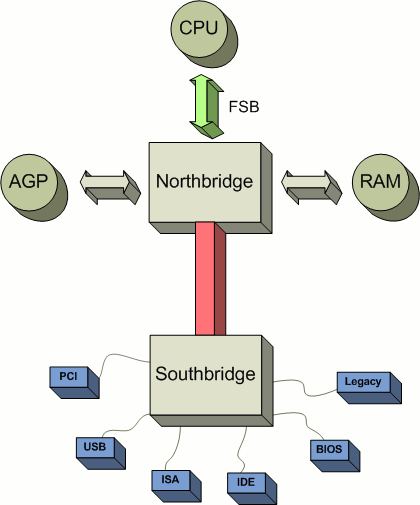
\includegraphics[keepaspectratio,width=0.5\paperwidth]{Pictures/Schema_chipsatz.png}
	\end{center}
	\caption{主板芯片组}
	\label{fig:chipset}
\end{figure}

单芯片芯片组已推出多年,例如SiS 730。但直到最近nForce 4的出现才逐渐流行。现在的单芯片芯片组,不像以往般复杂,因Athlon 64已内建内存控制器,取代了北桥的功能。纵使芯片组变成单芯片,习惯上亦沿用旧名称。

北桥(英语:Northbridge)是基于Intel处理器的个人电脑主板芯片组两枚芯片中的一枚,北桥设计用来处理高速信号,通常处理中央处理器、随机存取存储器、AGP或PCI Express的端口,还有与南桥之间的通信。


传统的北桥内建内存控制器,让处理器连接前端总线,而处理器和内存总线则跑相同的时脉。随后,芯片组分开处理器和内存总线的频率,让前端总线只代表处理器和北桥之间的通道。

北桥留下来的只剩下AGP或PCI Express控制器和与南桥通信,有时北桥会和南桥整合在同颗芯片中,有一些北桥则连绘图处理器也整合进去,而另外支援AGP或PCI Express接口。整合式北桥会侦测到附加在AGP插槽上有安装显卡,并停止其绘图处理器功能,但有些北桥可以允许同时使用整合式显卡和安装外加显卡,作为多显示输出。

Intel Hub Architecture(IHA)可用来取代南桥与北桥,IHA芯片组亦分成二大项:Graphics和AGP Memory Controller Hub (GMCH)与I/O Controller Hub (ICH)。

AMD在Athlon 64时代将内存总线整个拿掉,直接设计到处理器中,让北桥的功能只是支援外加显卡接口,例如AGP和PCI Express x16。由于北桥的重要性降低,有厂商索性将南北桥合并,成为单一芯片组,例如NVIDIA的nForce 4。这样可以减低芯片组的制造成本,但电脑的效能会降低。

南桥是基于Intel处理器的个人电脑主板芯片组两枚芯片中的一枚。南桥设计用来处理低速信号,通过北桥与CPU联系。各芯片组厂商的南桥名称都有所不同,例如英特尔称之为ICH,NVIDIA的称为MCP,ATI的称为IXP/SB。

南桥包含大多数周边设备接口、多媒体控制器和通讯接口功能。例如PCI控制器、ATA控制器、USB控制器、网络控制器、音效控制器。各世代的南桥效能大多雷同,但偶然听到某些南桥会有较差的Serial ATA或USB效能。

目前所有的南桥制造商都提供SATA磁盘阵列功能,NVIDIA则允许SATA和ATA硬盘机混合组成磁盘阵列。最新的英特尔Matrix RAID技术,让RAID-0和RAID-1组态可以在两颗硬盘机中同时使用。

大多数南桥都能直接连接Gigabit Lan PHY(实体层芯片,用来处理连接讯号),高阶的南桥通常拥有两组Gigabit Lan PHY,不过中阶的主板则只支援一组。而NVIDIA最新的南桥则支援带宽合并、封包排序和TCP/IP加速等高级网络卡功能。现在大部份高级南桥则支援Azalia高传真音效,借着编码芯片支援7.1声道音效。

大多数南桥都支援PCI Express Hub,但主板制造商通常采用北桥所提供的PCI Express Lane。
\subsection{前端总线}
前端总线(FSB,Front Side Bus)是指中央处理器数据总线的专门术语,此总线负责中央处理器和北桥芯片间的数据传递。如图\ref{fig:mainboard}。

\begin{figure}[htb]
\centering
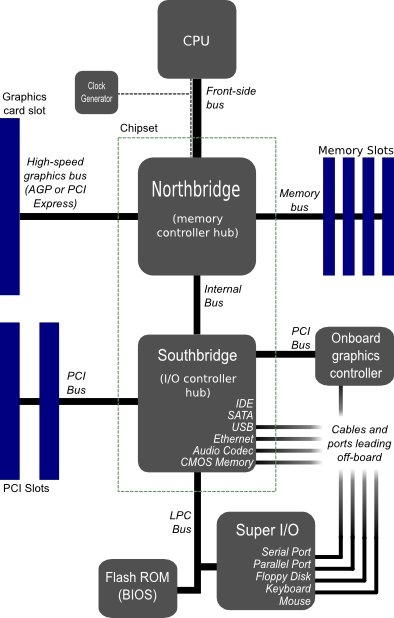
\includegraphics[keepaspectratio,width=0.5\paperwidth]{Pictures/Motherboard_diagram.jpg}
\caption{典型的PC主板}
\label{fig:mainboard}
\end{figure}
某些带有L2和L3缓存(Cache)的计算机,通过后端总线(Back Side Bus)实现这些缓存和中央处理器的连接,而此总线的数据传输速率总是高于前端总线。

大多数现代总线(GTL+和EV6)是CPU和芯片组的连接主干。芯片组(通常由南桥和北桥组成)是和系统中其他总线的连接节点。PCI、AGP和内存总线均和芯片组相连,以使设备间数据能相互传送。

这些第二级系统总线的运行速率取决于前端总线的速率。总之,高的前端总线速率意味着计算机的高处理性能。

在PC发展初期,由于处理器速度不高,大部份元件的时脉均保持同步,直至80486时代,在处理器制程持续进步下,处理器速度也加速成长,当时由于其他外部元件受电气结构所限,而无法跟进成长,因此Intel首次于处理器时脉中加入倍频设计,首颗处理器为Intel 80486DX2,外部传输时脉是处理器的一半,及后处理器成长速度仍远超过外部元件,两者速度差距越来越大。直至Pentium III时代,处理器时脉已超越1GHz,但外部传输时脉仍仅有133MHz。

正常来说,外频速度越高代表处理器在同一周期下可读写越多的数据,因此,外频速度很可能会变成系统效能上的瓶颈,为解决处理器带宽不足的问题,Intel于Pentium 4时代加入Quad Pumped Bus架构,使其在同一周期内可传送4笔数据,此举令外部传输时脉不变下,传输效率却可提升四倍。

\subsection{内频与总线速率}
中央处理器的时脉速度(简称内频)由系统总线速率(bus speed)乘上倍频系数决定。例如,一个时脉速度为 700MHz 的处理器,可能运行于 100MHz 的系统总线上。这说明处理器内的时钟倍频器的倍率设置为7,即中央处理器被设定为以7倍于系统总线的速率运行:100 MHz×7 = 700 MHz。通过改变倍频系数或系统总线速率,可以得到不同的时脉速度。以前经常套用的规则认为:时脉速度=外频(前端总线、FSB)*倍频系数。这句话严格来说并不正确。因为现在系统总线、前端总线(外频、FSB)速率不一样。就 Intel CPU 来说,前端总线=系统总线*4。所以,应该说时脉速度=系统总线*倍频系数。大多数主板允许用户通过跳线设置(BIOS)设定倍频或系统总线速率。现在许多处理器制造商预先锁定了处理器的倍频,但可以通过某些手段解锁。对所有的处理器,系统总线速率的适当提高可以增进其处理速率。

系统总线(BusSpeed)与前端总线(FSB、外频)的区别在于,前端总线(FSB、外频)的速度指的是CPU和北桥芯片间总线的速度。而系统总线(BusSpeed)的概念是建立在数位脉冲信号震荡速度基础之上的,也就是说,100MHz系统总线(BusSpeed)特指数位脉冲信号在每秒钟震荡一百万次,它更多的影响了PCI及其他总线的频率。之所以前端总线(FSB、外频)与系统总线(BusSpeed)这两个概念容易混淆,主要的原因是在以前的很长一段时间里,前端总线(FSB、外频)与系统总线(BusSpeed)是相同速率,因此往往直接称系统总线(BusSpeed)为外频,最终造成这样的误会。随着电脑技术的发展,人们发现前端总线频率(外频、FSB)需要高于系统总线(BusSpeed),因此采用了QDR(Quad Date Rate)技术,或者其他类似的技术实现这个目的。这些技术的原理类似于AGP的2X或者4X,它们使得的前端总线(FSB、外频)频率成为系统总线(BusSpeed)的2倍、4倍甚至更高,从此之后系统总线(BusSpeed)和前端总线(FSB、外频)的区别才开始被人们重视起来。



\subsection{HyperTransport}

HyperTransport技术,简称“HT总线”,以前曾被称作“闪电数据传输”(Lightning Data Transport,LDT),是一种高速、双向、低延时、点对点的、串行或者并行的高带宽连接总线技术,于2001年4月2日开始投入使用。旨在提高个人计算机、服务器、嵌入式系统,以及网络和电信设备内集成电路之间的通信速度。该技术有助于减少系统之中的布线数量,从而能够减少系统瓶颈,让当前速度更快的微处理器能够更加有效地在高端多处理器系统中使用系统内存。由HyperTransport联合会(The HyperTransport Consortium)负责改进和发展此技术。AMD和全美达公司把这项技术应用在x86处理器上,而PMC-Sierra、Broadcom(博通)和Raza Microelectronics则把它应用在MIPS(一种RISC微处理器架构)微处理器上;除微处理器应用之外,AMD、NVIDIA、VIA和SiS把它用于PC主板的芯片组;惠普、Sun Microsystems、IBM、和IWill把它用于服务器领域;Cray、Newisys、 和QLogic把它用于高性能计算;CISCO Systems(思科)把它用于路由器领域。应该引起关注的是以上名单中唯独少了半导体巨头Intel,它继续选择使用一种共享的总线架构,但在Intel新的Nehalem架构(如Core i7)中内置了内存控制器。


具体应用有:
\begin{description}
	\item[替代前端总线]The primary use for HyperTransport is to replace the front-side bus, which is currently different for every type of machine. For instance, a Pentium cannot be plugged into a PCI Express bus. To expand the system, the proprietary front-side bus must connect through adapters for the various standard buses, like AGP or PCI Express. These are typically included in the respective controller functions, namely the northbridge and southbridge.

		In contrast, HyperTransport is an open specification, published by a multi-company consortium. A single HyperTransport adapter chip will work with a wide spectrum of HyperTransport enabled microprocessors. For example, Broadcom HT-1000 and HT-2000 server controller devices can work with many different HyperTransport enabled microprocessors.

		AMD uses HyperTransport to replace the front-side bus in their Opteron, Athlon 64, Sempron 64, Turion 64, Phenom, Phenom II and FX families of microprocessors.
	\item[多处理器]Another use for HyperTransport is as an interconnect for NUMA multiprocessor computers. AMD uses HyperTransport with a proprietary cache coherency extension as part of their Direct Connect Architecture in their Opteron and Athlon 64 FX (Dual Socket Direct Connect (DSDC) Architecture) line of processors. The HORUS interconnect from Newisys extends this concept to larger clusters. The Aqua device from 3Leaf Systems virtualizes and interconnects CPUs, memory, and I/O.
	\item[路由器和交换机]
	\item[协处理器连接]
	\item[扩展设备]
\end{description}


\begin{figure}[htb]
\centering
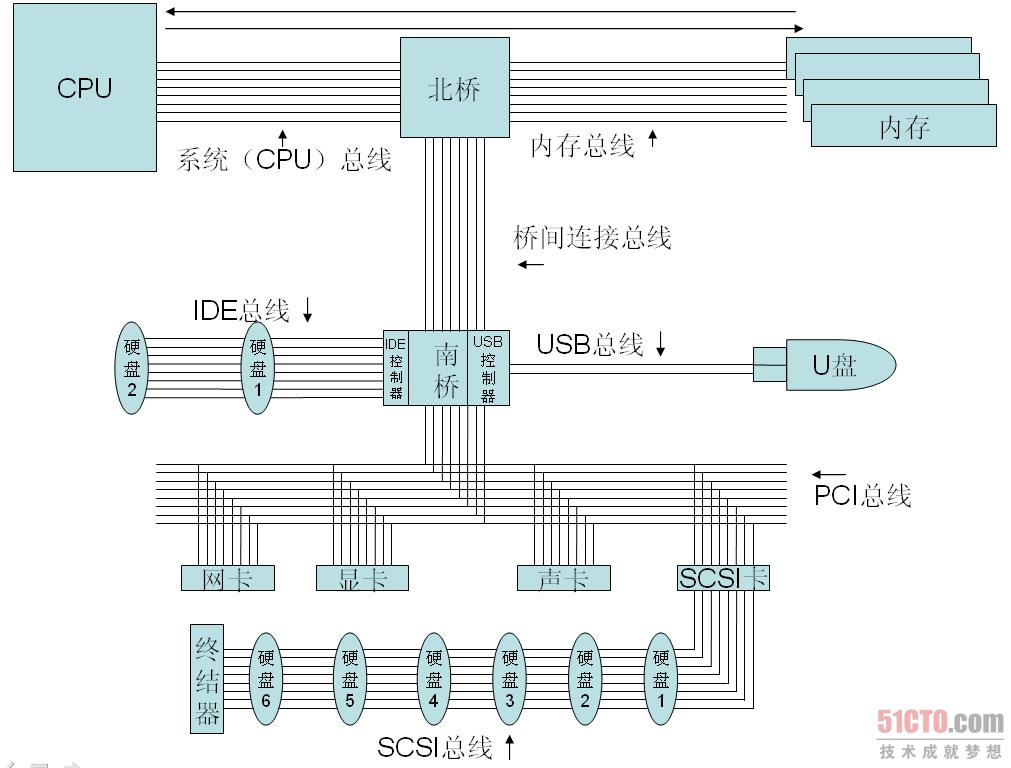
\includegraphics[keepaspectratio,width=0.5\paperwidth]{Pictures/g.jpg}
\caption{计算机总线图}
\label{fig:computerbuspic}
\end{figure}


\subsection{已过时的CNR插槽}
Communications and Networking Riser (CNR) is a slot found on certain PC motherboards and used for specialized networking, audio, and telephony equipment. A motherboard manufacturer can choose to provide audio, networking, or modem functionality in any combination on a CNR card. CNR slots were once commonly found on Pentium 4-class motherboards, but have since been phased out in favor of on-board or embedded components.














\section{OC速率}
Optical Carrier transmission rates are a standardized set of specifications of transmission bandwidth for digital signals that can be carried on Synchronous Optical Networking (SONET) fiber optic networks. Transmission rates are defined by rate of the bitstream of the digital signal and are designated by hyphenation of the acronym OC and an integer value of the multiple of the basic unit of rate, e.g., OC-48. The base unit is 51.84 Mbit/s. Thus, the speed of optical-carrier-classified lines labeled as OC-n is n × 51.84 Mbit/s.


\section{硬件测试相关知识}
\subsection{JTAG}
JTAG是联合测试工作组(Joint Test Action Group)的简称,是在名为标准测试访问端口和边界扫描结构的IEEE的标准1149.1的常用名称。此标准用于测试访问端口,使用边界扫描的方法来测试印刷电路板。

1990年JTAG正式由IEEE的1149.1-1990号文档标准化,在1994年,加入了补充文档对边界扫描描述语言(BSDL)进行了说明。从那时开始,这个标准被全球的电子企业广泛采用。边界扫描几乎成为了JTAG的同义词。

在设计印刷电路版时,目前最主要用在测试集成电路的副区块,而且也提供一个在嵌入式系统很有用的调试机制,提供一个在系统中方便的``后门''。当使用一些调试工具像电路内模拟器用JTAG当做讯号传输的机制,使得程式设计师可以经由JTAG去读取整合在CPU上的调试模组。调试模组可以让程式设计师调试嵌入式系统中的软件 。

\subsection{DUT}
被测器件(英语:device under test,DUT)或被测装置,又称在测单元或被测部件(unit under test,UUT),常用于表示正处于测试阶段的工业产品。
在半导体测试中,DUT表示晶圆或最终封装部件上的特定管芯小片。利用连接系统将封装部件连接到手动或自动测试设备(ATE),ATE会为其施加电源,提供模拟信号,然后测量和估计器件得到的输出,以这种方式测定特定被测器件的好坏。

对于晶圆来说,使用者需要将ATE用一组显微针连接到一个个独立的DUT(晶圆小片)。若晶圆已被切割成小片并封装,我们可以用ZIF插座(零插拔力插座)将ATE连接到DUT(管壳)上。

更多的情况下,DUT用于表示任何被测电子装置。例如,装配线下线的手机中的每一芯片都会被测试,而手机整机会以同样的方式进行最终的测试,这里的每一部手机都可以被称作DUT。

DUT常以测试针组成的针床测试台连接到ATE。

被测系统(System under test,SUT)表示正在被测试的系统,目的是测试系统是否能正确操作。这一词语常用于软件测试中。

软件系统测试的一个特例是对应用软件的测试,称为被测应用程序(application under test,AUT)。

SUT也表明软件已经到了成熟期,因为系统测试在测试周期中是集成测试的后一阶段。

\chapter{系统软件}
\section{字符编码}

\subsection{ASCII与ISO/IEC 646}
ASCII(American Standard Code for Information Interchange,美国信息交换标准代码)是基于拉丁字母的一套电脑编码系统。它主要用于显示现代英语,而其扩展版本EASCII则可以勉强显示其他西欧语言。它是现今最通用的单字节编码系统(但是有被Unicode追上的迹象),并等同于国际标准ISO/IEC 646。ISO/IEC 646是国际标准化组织(ISO)和国际电工委员会(IEC)于1972年制订的标准。它是一个 7-位元字符的字集,来自数个国家标准,最主要来自美国的 ASCII(美国信息互换标准代码)。

ASCII第一次以规范标准的型态发表是在1967年,最后一次更新则是在1986年,至今为止共定义了128个字符;其中33个字符无法显示(这是以现今操作系统为依归,但在DOS模式下可显示出一些诸如笑脸、扑克牌花式等8-bit符号),且这33个字符多数都已是陈废的控制字符。控制字符的用途主要是用来操控已经处理过的文字。在33个字符之外的是95个可显示的字符,包含用键盘敲下空白键所产生的空白字符也算1个可显示字符(显示为空白)。

\subsection{ISO 8859}
ISO 8859,全称ISO/IEC 8859,是国际标准化组织(ISO)及国际电工委员会(IEC)联合制定的一系列8位字符集的标准,现时定义了15个字符集。这15个字符集是互斥的。如Latin-1和Latin-2而言相同数字代表不同字符。除了使用拉丁字母的语言外,使用西里尔字母的东欧语言、希腊语、泰语、现代阿拉伯语、希伯来语等,都可以使用这个形式来储存及表示。

ISO 8859-1,正式编号为ISO/IEC 8859-1:1998,又称Latin-1或“西欧语言”,是国际标准化组织内ISO/IEC 8859的第一个8位字符集。它以ASCII为基础,在空置的0xA0-0xFF的范围内,加入96个字母及符号,藉以供使用附加符号的拉丁字母语言使用。

ISO 8859-2,正式编号为ISO/IEC 8859-2:1999,又称Latin-2或“中欧语言”,是国际标准化组织内ISO/IEC 8859的其中一个8位字符集。

ISO 8859-15字符集,也称为 Latin-9,或者被匿称为 Latin-0,它将 Latin-1中较少用到的符号删除,换成当初遗漏的法文和芬兰字母;还有,把英镑和日元之间的金钱符号,换成了欧盟货币符号。

\subsection{通用字符集}
通用字符集(Universal Character Set,UCS)是由ISO制定的ISO 10646(或称ISO/IEC 10646)标准所定义的标准字符集。通用字符集是所有包括了其他字符集。它保证了与其他字符集的双向兼容,即,如果你将任何文本字符串翻译到UCS格式,然后再翻译回原编码,你不会丢失任何信息。UCS包含了已知语言的所有字符。除了拉丁语、希腊语、斯拉夫语、希伯来语、阿拉伯语、亚美尼亚语、格鲁吉亚语,还包括中文、日文、韩文这样的方块文字,UCS还包括大量的图形、印刷、数学、科学符号。ISO/IEC 10646定义了一个31位的字符集。ISO/IEC 10646-1标准第一次发表于1993年,现在的公开版本是ISO/IEC 10646-1:2000。ISO/IEC 10646-2在2001年发表。

UCS不仅给每个字符分配一个代码,而且赋予了一个正式的名字。表示一个UCS或Unicode值的十六进制数通常在前面加上“U+”,例如“U+0041”代表字符“A”。

\subsection{Unicode}
位于美国加州的Unicode组织允许任何愿意支付会员费用的公司或是个人加入,其成员包含了主要的电脑软硬件厂商,例如奥多比系统、苹果公司、惠普、IBM、微软、施乐等。20世纪80年代末,组成Unicode组织的商业机构,和国际合作的国际标准化组织(International Organization for Standardization,简称ISO)因为电脑普及和资讯国际化的前提下,分别各自成立了Unicode组织和ISO-10646工作小组。他们不久便发现对方机构的存在,大家为着相同的目的而工作,于是两个组织便共同合作开发适用于各国语言的通用码,而且“相当有默契地”各自发表Unicode和ISO-10646字集。虽然实际上两者的字集编码相同,但实质上两者确实为两个不同的标准。

目前,几乎所有电脑系统都支持基本拉丁字母,并各自支持不同的其他编码方式。Unicode为了和它们相互兼容,其首256字符保留给ISO 8859-1所定义的字符,使既有的西欧语系文字的转换不需特别考量;并且把大量相同的字符重复编到不同的字符码中去,使得旧有纷杂的编码方式得以和Unicode编码间互相直接转换,而不会遗失任何资讯。

目前实际应用的统一码版本对应于UCS-2,使用16位的编码空间。也就是每个字符占用2个字节。上述16位统一码字符构成基本多文种平面(Basic Multilingual Plane,简称BMP),包含了常见的CJK字。最新(但未实际广泛使用)的统一码版本定义了16个辅助平面,两者合起来至少需要占据21位的编码空间,比3字节略少。但事实上辅助平面字符仍然占用4字节编码空间,与UCS-4保持一致。目前辅助平面的工作主要集中在第二和第三平面的中日韩统一表意文字中,因此包括GBK、GB18030、Big5等简体中文、繁体中文、日文、韩文以及越南喃字的各种编码与Unicode的协调性被重点关注。

Unicode的码空间从U+0000到U+10FFFF,共有1,112,064个码位(code point)可用来映射字符. Unicode的码空间可以划分为17个平面(plane),每个平面包含216(65,536)个码位。每个平面的码位可表示为从U+xx0000到U+xxFFFF, 其中xx表示十六进制值从0016 到1016,共计17个平面。第一个平面成为基本多文种平面(Basic Multilingual Plane, BMP),或称第零平面(Plane 0)。其他平面称为辅助平面(Supplementary Planes)。基本多语言平面内,从U+D800到U+DFFF之间的码位区段是永久保留不映射到字符,因此UTF-16利用保留下来的0xD800-0xDFFF区段的码位来对辅助平面的字符的码位进行编码。

Unicode依随着UCS的标准而发展。目前最新的版本为第六版,已收入了超过十万个字符(第十万个字符在2005年获采纳)。Unicode备受认可,并广泛地应用于电脑软件的国际化与本地化过程。有很多新科技,如XML、Java,以及现代的操作系统,都采用Unicode编码。

\subsection{UTF}
Unicode的实现方式不同于编码方式。一个字符的Unicode编码是确定的。但是在实际传输过程中,由于不同系统平台的设计不一定一致,以及出于节省空间的目的,对Unicode编码的实现方式有所不同。Unicode的实现方式称为Unicode转换格式(Unicode Transformation Format,简称为UTF)。

例如,如果一个仅包含基本7位ASCII字符的Unicode文件,如果每个字符都使用2字节的原Unicode编码传输,其第一字节的8位始终为0。这就造成了比较大的浪费。对于这种情况,可以使用UTF-8编码,这是一种变长编码,它将基本7位ASCII字符仍用7位编码表示,占用一个字节(首位补0)。而遇到与其他Unicode字符混合的情况,将按一定算法转换,每个字符使用1-3个字节编码,并利用首位为0或1进行识别。这样对以7位ASCII字符为主的西文文档就大大节省了编码长度。类似的,对未来会出现的需要4个字节的辅助平面字符和其他UCS-4扩充字符,2字节编码的UTF-16也需要通过一定的算法进行转换。再如,如果直接使用与Unicode编码一致(仅限于BMP字符)的UTF-16编码,由于每个字符占用了两个字节,在麦金塔电脑 (Mac)机和个人电脑上,对字节顺序的理解是不一致的。

目前在PC机上的Windows系统和Linux系统对于UTF-16编码默认使用UTF-16 LE。此外Unicode的实现方式还包括UTF-7、Punycode、CESU-8、SCSU、UTF-32、GB18030等,这些实现方式有些仅在一定的国家和地区使用,有些则属于未来的规划方式。目前通用的实现方式是UTF-16小端序(LE)、UTF-16大端序(BE)和UTF-8。

\subsection{UTF-8}
UTF-8(8-bit Unicode Transformation Format)是一种针对Unicode的可变长度字符编码(定长码),也是一种前缀码。它可以用来表示Unicode标准中的任何字符,且其编码中的第一个字节仍与ASCII相容,这使得原来处理ASCII字符的软件无须或只须做少部份修改,即可继续使用。因此,它逐渐成为电子邮件、网页及其他储存或传送文字的应用中,优先采用的编码。互联网工程工作小组(IETF)要求所有互联网协议都必须支持UTF-8编码。互联网邮件联盟(IMC)建议所有电子邮件软件都支持UTF-8编码。

UTF-8使用一至四个字节为每个字符编码:128个US-ASCII字符只需一个字节编码(Unicode范围由U+0000至U+007F)。带有附加符号的拉丁文、希腊文、西里尔字母、亚美尼亚语、希伯来文、阿拉伯文、叙利亚文及它拿字母则需要二个字节编码(Unicode范围由U+0080至U+07FF)。其他基本多文种平面(BMP)中的字符(这包含了大部分常用字)使用三个字节编码。其他极少使用的Unicode 辅助平面的字符使用四字节编码。

每个使用UTF-8储存的字符,除了第一个字节外,其余字节的头两个位元都是以"10"开始,使文字处理器能够较快地找出每个字符的开始位置。在ASCII码的范围,用一个字节表示。大于ASCII码的,就会由上面的第一字节的前几位表示该unicode字符的长度,比如110xxxxxx前三位的二进制表示告诉我们这是个2BYTE的UNICODE字符;1110xxxx是个三位的UNICODE字符,依此类推;第一个字节的开头"1"的数目就是整个串中字节的数目。ASCII字母继续使用1字节储存,重音文字、希腊字母或西里尔字母等使用2字节来储存,而常用的汉字就要使用3字节。辅助平面字符则使用4字节。


\subsection{UTF-16}
UTF-16是Unicode字符集的一种转换方式,即把Unicode的码位转换为16比特长的码元序列,以用于数据存储或传递。UTF-16正式定义于ISO/IEC 10646-1的附录C。

BMP内,从U+D800到U+DFFF之间的码位区段是永久保留不映射到字符,因此UTF-16利用保留下来的0xD800-0xDFFF区段的码位来对辅助平面的字符的码位进行编码。

从U+0000至U+D7FF以及从U+E000至U+FFFF的码位,UTF-16与UCS-2编码这个范围内的码位为单个16比特长的码元,数值等价于对应的码位. BMP中的这些码位是仅有的码位可以在UCS-2被表示.从U+10000到U+10FFFF的码位为辅助平面(Supplementary Planes)中的码位,在UTF-16中被编码为一对16比特长的码元(即32bit,4Bytes),称作代理对(surrogate pair)。

UTF-16的大尾序和小尾序储存形式都在用。一般来说,以Macintosh制作或储存的文字使用大尾序格式,以Microsoft或Linux制作或储存的文字使用小尾序格式。

\subsection{大小端和BOM}

字节序,又称端序,尾序(英语:Endianness)。在计算机科学领域中,字节序是指存放多字节数据的字节(byte)的顺序,典型的情况是整数在内存中的存放方式和网络传输的传输顺序。Endianness有时候也可以用指位序(bit)。一般而言,字节序指示了一个UCS-2字符的哪个字节存储在低地址。如果LSByte在MSByte的前面,即LSB为低地址,则该字节序是小端序;反之则是大端序。

网络传输一般采用大端序,也被称之为网络字节序,或网络序。IP协议中定义大端序为网络字节序。

字节顺序标记(英语:byte-order mark,BOM)是位于码点U+FEFF的统一码字符的名称。当以UTF-16或UTF-32来将UCS/统一码字符所组成的字串编码时,这个字符被用来标示其字节序。它常被用来当做标示文件是以UTF-8、UTF-16或UTF-32编码的记号。

统一码中,值为U+FFFE的码位被保证将不会被指定成一个统一码字符。这意味着0xFF、0xFE将只能被解释成小尾序中的U+FEFF。

字节顺序标记U+FEFF字符在UTF-8中被表示为序列EF BB BF。许多Windows程序(包括Windows记事本)在UTF-8编码的档案的开首加入一段字节串EF BB BF。这是字节顺序记号U+FEFF的UTF-8编码结果。对于没有预期要处理UTF-8的文字编辑器和浏览器会显示成ISO-8859-1字符串""。

\subsection{汉字内码}

在计算机科学及相关领域当中,内码指的是“将资讯编码后,透过某种方式储存在特定记忆装置时,装置内部的编码形式”。在以往的英文系统中,内码为ASCII。 在繁体中文系统中,目前常用的内码为大五码。在简体中文系统中,内码则为国标码。为了软件开发方便,如国际化与在地化,现在许多系统会使用统一码做为内码,常见的Windows、麦金塔、Linux皆如此。许多语言也采用统一码为内码,如Java、Python 3。

内码是指整机汉字系统中使用的二进制字符编码,是沟通输入、输出与系统平台之间的交换码,通过内码可以达到通用和高效率传输文本的目的。比如MS Word中所存储和调用的就是内码而非图形文字。英文ASCII 字符采用一个字节的内码表示,中文字符如国标字符集中,GB2312、GB12345、GB13000皆用双字节内码,GB18030(27,533汉字)双字节内码汉字为20,902个,其余6,631个汉字用四字节内码。

汉字内码主要有:GB码(1980年国家公布的简体汉字编码方案,在大陆、新加坡得到广泛的使用,也称国标码),GBK码(简体版的Win95和Win98都是使用GBK作系统内码),BIG5码(针对繁体汉字的汉字编码,目前在台湾、香港的电脑系统中得到普遍应用),HZ码(在Internet上广泛使用的一种汉字编码),ISO-2022CJK码,Unicode码。

\subsection{GB2312与区位码}
GB 2312 或 GB 2312-80 是中国国家标准简体中文字符集,全称《信息交换用汉字编码字符集·基本集》,又称GB0,由中国国家标准总局发布,1981年5月1日实施。GB2312编码通行于中国大陆;新加坡等地也采用此编码。中国大陆几乎所有的中文系统和国际化的软件都支持GB 2312。GB 2312标准共收录6763个汉字,覆盖中国大陆99.75\%的使用频率同时收录了包括拉丁字母、俄语西里尔字母在内的682个字符。对于人名、古汉语等方面出现的罕用字,GB 2312不能处理,这导致了后来GBK及GB 18030汉字字符集的出现。

GB 2312中对所收汉字进行了“分区”处理,每区含有94个汉字/符号。这种表示方式也称为区位码。01-09区为特殊符号。16-55区为一级汉字,按拼音排序。56-87区为二级汉字,按部首排序。10-15区及88-94区则未有编码。举例来说,“啊”字是GB2312之中的第一个汉字,它的区位码就是1601。国标码是一个四位十六进制数,区位码是一个四位的十进制数,每个国标码或区位码都对应着一个唯一的汉字或符号,但因为十六进制数我们很少用到,所以大家常用的是区位码,它的前两位叫做区码,后两位叫做位码。

EUC-CN是GB 2312最常用的表示方法,兼容ASCII。浏览器编码表上的“GB2312”,通常都是指“EUC-CN”表示法。GB 2312非ASCII字符使用两个字节来表示。“第一位字节”使用0xA1-0xF7,“第二位字节”使用0xA1-0xFE.举例来说,“啊”字的区位码是1601。在EUC-CN之中,它把0xA0+16=0xB0,0xA0+1=0xA1,得出0xB0A1。

HZ is another encoding of GB2312 that is used mostly for Usenet postings.

Compared to UTF-8, GB2312 (whether native or encoded in EUC-CN) is more storage efficient, this because no bits are reserved to indicate three or four byte sequences, and no bit is reserved for detecting tailing bytes.

\subsection{微软GBK}
GBK即汉字内码扩展规范,K为汉语拼音 Kuo Zhan(扩展)中“扩”字的声母。
1993年,Unicode 1.1版本推出,收录中国大陆、台湾、日本及韩国通用字符集的汉字,总共有20,902个。中国大陆订定了等同于Unicode 1.1版本的“GB13000.1-93”“信息技术通用多八位编码字符集(UCS)第一部分:体系结构与基本多文种平面”。

微软利用GB 2312-80未使用的编码空间,收录GB 13000.1-93全部字符制定了GBK编码。根据微软资料,GBK是对GB2312-80的扩展,也就是CP936字码表 (Code Page 936)的扩展(之前CP936和GB 2312-80一模一样),最早实现于Windows 95简体中文版。虽然GBK收录GB 13000.1-93的全部字符,但编码方式并不相同。GBK自身并非国家标准,只是曾由国家技术监督局标准化司、电子工业部科技与质量监督司公布为“技术规范指导性文件”。原始GB13000一直未被业界采用,后续国家标准GB18030技术上兼容GBK而非GB13000。

字符有一字节和双字节编码,00–7F范围内是一位,和ASCII保持一致,此范围内严格上说有96个文字和32个控制符号。之后的双字节中,前一字节是双字节的第一位。总体上说第一字节的范围是81–FE(也就是不含80和FF),第二字节的一部分领域在40–7E,其他领域在80–FE。

GBK向下完全兼容GB2312-80编码。 支持GB2312-80编码不支持的部分中文姓,中文繁体,日文假名,还包括希腊字母以及俄语字母等字母。不过这种编码不支持韩国字,也是其在实际使用中与unicode编码相比欠缺的部分。微软的CP936通常被视为等同GBK,连 IANA 也以“CP936”为“GBK”之别名。事实上比较起来, GBK 定义之字符较 CP936 多出95字。

\subsection{GB18030}
GB 18030,最新版本为GB 18030-2005,其全称为中华人民共和国国家标准GB 18030-2005《信息技术 中文编码字符集》,与GB 2312-1980完全兼容,与GBK基本兼容,支持GB 13000及Unicode的全部统一汉字,共收录汉字70244个。

此标准中,单字节的部分收录了GB/T 11383-1989的0x00到0x7F全部128个字符。双字节部分采用两个八位二进制位串表示一个字符,其首字节码位从0x81至0xFE,尾字节码位分别是0x40至0x7E和0x80至0xFE。四字节部分采用GB/T 11383-1989未采用的0x30至0x39作为对双字节编码的扩充的后缀。这样扩充的四字节编码,其范围为0x81308130到0xFE39FE39。四字节字符的第一个字节的编码为0x81至0xFE;第二个字节的编码范围为0x30至0x39;第三个字节编码范围为0x81至0xFE;第四个字节编码范围为0x30至0x39。

GB18030与Unicode的关系:GB 18030是一种对字符集的多字节编码格式,相当于UTF-8(对Unicode码点(code point)的编码传输格式),而且都是向后兼容ASCII,并且能表示所有的Unicode码点。GB 18030的四字节编码共有1,587,600 (126×10×126×10), 足以覆盖Unicode的1,111,998 (17×65536 − 2048 surrogates − 66 noncharacters)码点。此外,GB18030还向后兼容了GB 2312与GBK编码。与Unicode码点的映射关系(mapping)一部分要查表,其它可以通过算法求出,这与UTF-8相比不够方便。


\subsection{ISO 2022}

全称ISO/IEC 2022,由国际标准化组织(ISO)及国际电工委员会(IEC)联合制定,是一个使用7位编码表示汉语文字、日语文字或朝鲜文字的方法。
ISO 2022等同于欧洲标准组织(ECMA)的ECMA-35、中国国标GB 2312、日本工业规格JIS X 0202(旧称JIS C 6228)及韩国工业规格KS X 1004(旧称KS C 5620)。拉丁字母、希腊字母、西里尔字母、希伯来字母等的语文,由于只使用数十个字母,传统上均使用8位编码的ISO/IEC 8859标准来表示。但由于汉语、日语及朝鲜语字数众多,无法用单一个8位字符来表达,故需要多于一个字节来代表一个字。于是,ISO 2022就设计出来让汉语、日语及朝鲜语可以使用数个7位编码的字符来示。ISO 2022使用“逃逸字串”(Escape sequence)。逃逸字串由1个“ESC”字符(0x1B),再由两至三个字串组成。此标记代表它后面的字符,属于下表字符集的文字。





























\section{数字证书}
1.带有私钥的证书
由Public Key Cryptography Standards \#12,PKCS\#12标准定义,包含了公钥和私钥的二进制格式的证书形式,以pfx作为证书文件后缀名。

2.二进制编码的证书
证书中没有私钥,DER 编码二进制格式的证书文件,以cer作为证书文件后缀名。

3.Base64编码的证书
证书中没有私钥,BASE64 编码格式的证书文件,也是以cer作为证书文件后缀名。
由定义可以看出,只有pfx格式的数字证书是包含有私钥的,cer格式的数字证书里面只有公钥没有私钥。
在pfx证书的导入过程中有一项是“标志此密钥是可导出的。这将您在稍候备份或传输密钥”。一般是不选中的,如果选中,别人就有机会备份你的密钥了。如果是不选中,其实密钥也导入了,只是不能再次被导出。这就保证了密钥的安全。
如果导入过程中没有选中这一项,做证书备份时“导出私钥”这一项是灰色的,不能选。只能导出cer格式的公钥。如果导入时选中该项,则在导出时“导出私钥”这一项就是可选的。
如果要导出私钥(pfx),是需要输入密码的,这个密码就是对私钥再次加密,这样就保证了私钥的安全,别人即使拿到了你的证书备份(pfx),不知道加密私钥的密码,也是无法导入证书的。相反,如果只是导入导出cer格式的证书,是不会提示你输入密码的。因为公钥一般来说是对外公开的,不用加密
\section{大小端}

如果LSByte在MSByte的前面,即LSB为低地址,则该字节序是小端序;反之则是大端序。A big-endian machine stores the most significant byte first, and a little-endian machine stores the least significant byte first. 

网络传输一般采用大端序,也被称之为网络字节序,或网络序。IP协议中定义大端序为网络字节序。

Linux和Windows使用小尾端。Macintosh使用大端序。

\section{字体基础知识}

\subsection{字库标准}
PostScript(PS)是主要用于电子产业和桌面出版领域的一种页面描述语言和编程语言。
桌面出版系统使用的字库有两种标准: PostScript字库和truetype字库。这两种字体标准都是采用曲线方式描述字体轮廓,因此都可以输出很高质量的字形。TrueType最初是由苹果公司引入,用以回应Adobe专有的PostScript格式。早期的TrueType字体多为PostScript字体的拙劣翻版,但时至今日,各大字体公司都以TrueType格式来发布他们的产品(其中有些是有PostScript原型的,有些则原生就是TrueType,再无其他格式)。早在80年代末,苹果公司为了对抗Adobe公司的Type 1 PostScript字体,设计开发了TrueType,之后微软加入了开发,后来视窗系统的字体格式基本上都统一成TrueType,而在苹果的麦金塔系统中却成了PostScript和TrueType对立的局面。TrueType后来也被Linux等系统使用,成为标准字体。TrueType的主要强项在于它能给开发者提供关于字体显示、不同字体大小的像素级显示等的高级控制。在新开发的OpenType类型字体中,可以选择PostScript还是TrueType作为记述方式。

TrueType字体,中文名称全真字体。TrueType是由Apple公司和Microsoft公司联合提出的一种新型数学字形描述技术。它用数学函数描述字体轮廓外形,含有字形构造、颜色填充、数字描述函数、流程条件控制、栅格处理控制、附加提示控制等指令。其采用几何学中二次B样条曲线及直线来描述字体外形轮廓,特点是:TrueType既可作打印字体,又可用作屏幕显示;由于它用指令对字形进行描述,因此它与分辨率无关,输出时总是按打印机分辨率输出。无论放大或缩小,字符总是光滑的,不会有锯齿出现。但相对PostScript字体来说,其质量要差一些。特别是在文字太小时,就表现得不是很清楚。truetype字便宜,字款丰富。但一般情况厂truetype字不能直接由rip输出。需要经过特殊处理,比如转成曲线或输出时下载,使用起来较麻烦。速度也要慢一些,尤其是处理大量文字时很不方便,因此不适合用来作为页面的正文文字使用。

PostScript汉字库分为显示字库和打印字库,显示字库安装在制作计算机上,用来制作版面时显示用,通常由低分辨率的点阵字构成。打印字库要挂接在rip上,在解释页面时由rip把需要的字库调入页面并解释成记录的点阵。 PostScript汉字使用方便,输出速度快,是输出中心必备的。

TrueType vs. PostScript:TrueType有着更好的hinting属性,如果定义了hinting的话。这是一个小陷阱:必须要有人愿意为这些特性编写代码。Hinting是一种技术,用于数字化字体的平滑显示。它负责在小字号下处理矢量数据并将其转换为像素,以精确的显示字体;可以把hinting视作一种抗锯齿技术。这是另一个陷阱:hinting仅仅在屏幕小字号显示时才有用武之地。

TrueType并非不可以印刷,之所以不适合用于高端印刷,是因为打印机必须将TrueType矢量数据转换成PostScript语言。但不幸的是,PostScript不象TrueType那样支持如此多的曲线段 。
TrueType 使用二次曲线(quadratic curves)。和你在 Illustrator 和 Photoshop 中绘图时所用的曲线不同,二次曲线需要4个点来定义一条曲线。PostScript 使用三次曲线(cubic curves)。这是我们所熟悉的曲线,我们第一次在Illustrator 或 Photoshop 中理解和学习钢笔工具还是一个痛苦的回忆,但现在我们已经是轻车熟路了。三次曲线只需要3个点就可以定义一条曲线。对吧?因为三次方的意思就是自乘3次(其实应该是两次..译注),一个立方体就是3D。当TrueType 转换为 PostScript的时候,不是所有的二次曲线都能够转换为平滑的三次曲线。

OpenType,是一种可缩放字型(scalable font)电脑字体类型,采用PostScript格式,是美国微软公司与Adobe公司联合开发,用来替代TrueType字型的新字型。这类字体的文件扩展名为.otf,类型代码是OTTO,现行标准为OpenType 1.4。OpenType最初发表于1996年,并在2000年之后出现大量字体。它源于微软公司的TrueType Open字型,TrueType Open字型又源于TrueType字型。OpenType font包括了Adobe CID-Keyed font技术。Adobe公司已经在2002年末将其字体库全部改用OpenType格式。到2005年大概有一万多种OpenType字体,Adobe产品占了三分之一。

结论?使用Open Type格式,因为它可以同时嵌入TrueType 和 PostScript信息,同时它又是跨平台兼容的。全世界最棒!加油Adobe和Microsoft!听完我上面的解释,你应该能理解为什么要使用Open Type格式而不是其他格式了吧?如果你还想知道OpenType格式为什么如此优秀,看看这段引自Thomas Phinney的文章TrueType vs. PostScript Type 1中的描述:OpenType 将 PostScript 或 TrueType 轮廓都放入一个 TrueType 风格的“包装袋”中。应用程序和大多数的操作系统都在这个字体的子系统之外操作,不再关心这个“包装袋”中装的是什么类型的字体。

\subsection{ClearType技术}
ClearType,是由美国微软公司在其视窗操作系统中提供的屏幕亚像素微调字体平滑工具,让Windows字体更加漂亮。ClearType主要是针对LCD液晶显示器设计,可提高文字的清晰度。基本原理是,将显示器的R, G, B各个次像素也发光,让其色调进行微妙调整,可以达到实际分辨率以上(横方向分辨率的三倍)的纤细文字的显示效果。Windows上的像素和显示器上的像素对应的液晶显示器上效果最为明显,使用阶调控制一般CRT显示器上也可以得到一些效果。在Windows XP平台上,这项技术默认是关闭,到了Internet Explorer 7才默认为开启。而与ClearType几乎同样的技术在苹果电脑的Mac OS操作系统中,早在1998年发布的Mac OS 8.5就已经使用了。另外,依靠ClearType技术提高字体的可读性,相当程度上依赖于使用的字体,所以和原有的标准抗锯齿技术不能进行单纯比较。如果显示器不具有适用于ClearType的像素组合特性,以ClearType显示文字的实际效果会比使用前还要差。大多Windows默认的中文字体在显示小文字时使用点阵来显示,不使用ClearType。微软在Windows Vista里,新发布了两个ClearType中文字体:微软雅黑和微软正黑体。

为什么英文矢量字体就可以直接使用 ClearType 来进行平滑显示呢?这是因为大多数优秀的英文字体并不是采用内嵌点阵的方式来进行优化的,它们采用的是一种叫做 Hinting (字形微调)的技术来对小字号的显示进行优化。
  我们知道,矢量字体是可以无限平滑缩放的,在使用的时候,要通过操作系统的字体引擎自动的解析渲染为实际的像素,才能够在屏幕上显示出来。但是在字号很小的时候,由于能使用的像素非常有限,这种自动解析会出现很多问题,例如笔画粗细不匀,文字之间高低不齐,甚至笔画模糊无法识别等。因此必须由字体设计师人工干预,在矢量字库中嵌入一些附加的提示信息,来告诉字体渲染引擎在某个特定的字号下面,应该如何对这个字符的细节进行修正,才能准确的显示。这种在矢量字体中嵌入的提示信息,就叫做 Hinting 。
  对于中文字体来说,这种提示就更为重要,因为中文的笔画繁多,自动解析的错误也就更多更严重。在字号更小的情况下,根本无法显示全部的笔画,这时候还需要设计师在不影响整体的情况下,对笔画进行取舍,去掉一些不影响识别的笔画,否则这个文字就会因糊成一团无法识别。 Hinting 调整的范围需要涵盖各级小字号,一般最少要包括 9px - 18px 这个常用的字号区间。这种 Hinting ,即使是对于非常有经验的设计师,也是非常高难度而且费时费力的工作。

英文只有 26 个字母,但是对于中文的汉字情况就复杂的多了,仅仅是最常用的汉字就有 6000 个,然后为了在简繁体混排时候能完美的显示,就必须同时包含繁体和简体两套字符,再加上众多的不常用但是会在古籍文献中非常重要的生僻字,一套比较完整的大字符集字库所包含的字符数目将接近 3 万个。仅仅是这矢量造字的工作就是非常浩大的。
  这还不算,作为一套功能完整的正文字体,还需要考虑到斜体和粗体的显示。所有的斜体状态,也同样必须由设计师对不同的字号指定不同的 Hinting ,否则就会有显示问题。为了更完美的显示粗体,微软决定将标准体和粗体分开,作为两套单独的字体来设计,安装时也是两套字体,但在系统中使用时是显示为一套字体的不同状态。这套单独的黑体也同样需要单独造字,然后指定一系列的 Hinting 和斜体 Hinting 。因此要开发一套优秀的中文大型字库,耗费的人力物力是惊人的。这也正是这套字体会如此昂贵的原因之一。

Hinting信息是评价一款优秀矢量字体的一个重要指标,良好的Hinting能在小字号下面提供和内嵌点阵字一样优秀的显示质量,同时又降低内存的消耗。虽然我们现在已经拥有不少不错的矢量中文字体,但适合屏幕显示的正文字体很少,而包含完善 Hinting 信息的,一个也没有。所以,如果要在中文 Vista 平台下彻底完美的实现文本的平滑显示,微软就必须全新开发一套具备完善Hinting信息的ClearType中文字体。

\subsection{字体文件格式}

TTF(TrueTypeFont)是Apple公司和Microsoft公司共同推出的字体文件格式,随着windows的流行,已经变成最常用的一种字体文件表示方式。ttc是microsoft开发的新一代字体格式标准,可以使多种truetype字体共享同一笔划信息,有效地节省了字体文件所占空间,增加了共享性。但是有些软件缺乏对这种格式字体的识别,使得ttc字体的编辑产生困难。两者的不同处是 TTC 档会含超过一种字型,例如繁体 Windows 的 Ming.ttc 就包含细明体及新细明体两种字型 (两款字型不同处只是英文固定间距),而 TTF 就只会含一种字型。TTC是几个TTF合成的字库,安装后字体列表中会看到两个以上的字体。两个字体中大部分字都一样时,可以将两种字体做成一个TTC文件,现在常见的TTC中的不同字体,汉字一般没有差别,只是英文符号的宽度不一样,以便适应不同的版面要求。


























\subsection{常见商业字体}
维基百科有条目:\href{http://en.wikipedia.org/wiki/List_of_CJK_fonts}{List of CJK fonts}

\begin{verbatim}
中易宋体&新宋体,即通常被熟知为宋体、新宋体的字体,是由北京中易中标电子信息技术有限公司制作并持有版权的两个TrueType字体。中易宋体&新宋体是随着简体中文版Windows和Microsoft Office一起分发的字体(文件名 Simsun.ttc)。Simsun一直是简体中文版Windows XP系统及之前版本的默认字体。但由于白体的特性,在Windows Vista中已经改用支持OpenType的微软雅黑。因为对于电脑显示器来说,应该选择黑体即无衬线体作为显示器字体,才有助于显示和阅读。此字体西文的半角字符部分由于采用等宽字体设计,被指衬线和笔画的比例太夸张而不便阅读。此宋体在8pt时已经无法正常地看清(即使打开了ClearType)。此外,宋体只有区区几个最佳字体大小,在某些大小时(如14pt及以上)会发现字的笔划有残缺、断裂、粗细不均的问题(若打开了ClearType的话,“横”仍然会看到有断裂的地方),这主要是字体没有加入Hinting信息的缘故。

中易黑体,Windows XP系统及之前版本中的默认黑体。通常被熟知为``黑体''的电脑字体其实是中易黑体,是由北京中易中标电子信息技术有限公司制作并持有版权的一种TrueType字体。中易黑体是随着简体中文版Windows和Microsoft Office一起分发的字体,文件名Simhei.ttc,目前版本为5.01。此字形同中易宋体的字形设计被指太琐碎,西文部分采用等宽字体,使得美感颇为降低。

微软雅黑是美国微软公司委托中国方正集团设计的一款全面支持ClearType技术的字体。蒙纳公司(Monotype Corporation)负责了字体的修飾(Hinting)工作。它属于OpenType类型,文件名是MSYH.TTF,在字体设计上属于无衬线字体和黑体。在使用ClearType功能的液晶显示器中,微软雅黑比以前Windows XP默认的中易宋体更加的清晰易读。

微软正黑体,微软公司的一款全面支援ClearType技术的TrueType 无衬线字体,用于繁体中文系统。随Windows Vista及Office 2007(繁体中文)一起发布,是Windows Vista缺省字体,在使用的ClearType功能的液晶显示器中,其比以前Windows XP缺省的新细明体更加清晰易读。中文世界里一套合适的 ClearType 屏幕正文显示字体字体必须能解决在 ClearType 平滑显示状态下小字号正常阅读的问题。现有的所有中文字库都无法在 ClearType 平滑显示状态下完美的文本显示。之前的宋体之所以能够在小字号点阵状态下很好的显示,是由于宋体在矢量字库中嵌入了 12 、 14 、 16 、 18 等几个点阵字库,才得以比较优秀的显示。但在 ClearType 状态下,继续采用这样内嵌点阵的方式来显示汉字,就会和平滑显示的英文粗细不一致,同时风格上非常的不协调。由于当初的宋体不是为平滑显示而设计的,强制平滑显示的效果就显得纤细发虚,看起来很模糊。

对于微软雅黑和微软正黑,不好简单的用简体或者繁体来区分他们,因为这两套字体都同时包含了比较完整的简繁体汉字,以确保在简体和繁体混排的页面上都能够完美的显示。但由于两岸的文教部门在各自的文字规范中对汉字的写法规定有很多细节上的不同,所以这两套字形在正式场合是不能混淆使用的。同样的,日文的Meiryo字体中也包含了大量的繁体汉字,不过由于汉字在日本也经过了上千年的演变,日文中的汉字写法和中国大陆和台湾也有着相当的区别。

华文细黑,是由中国常州华文印刷新技术有限公司(SinoType,找不到官网,不知是否倒闭)制作并持有版权的一种TrueType电脑字体。在无中文的环境下显示的名称为STHeiti Light或STXihei,它属于华文黑体系列字体之一。在设计上,它属于黑体或无衬线体。

华文宋体,常州华文印刷有限公司推出的字体。较平常的宋体相比,华文宋体在审美上有着新的开创与突破。目前,华文宋体已广泛应用到商标设计,广告设计,报纸与图书等行业中,效果较好。

威锋数位(DynaComware),原名华康科技(DynaLab),是台湾的电脑软件公司,为少数以电脑字型为主要开发产品的公司。自Windows 3.0推出时起,华康科技与微软公司合作将Windows中文化,并开始提供字型至今。繁体中文版Windows常用的细明体、新细明体及标楷体等皆由此公司制作提供。

RedHat发布Liberation系列,包含“Liberation Serif”“Liberation Sans”“Liberation Mono”三种字体,目标非常明确,就是取代微软的“Times New Roman”“Arial”“Courier New”。字形尺寸与微软的完全一样,所以用这三种字体代替微软的那三种不会导致文档排版的偏差与错乱。

   Nimbus系列,包含“Nimbus Roman No9 L”“Nimbus Sans L”“Nimbus Mono L”三种。目标直指Adobe的“Times”“Helvetica”“Courier”,主要供打印使用。与Liberation系列不同的是,其衬线看起来和微软的很接近,但尺寸不同。因为微软的那几款字体本来也就是针对Adobe的,字形和Adobe的几乎一样而尺寸却并没做到一样。

\end{verbatim}

















\section{字号}
px:pixel,像素,屏幕上显示的最小单位;1px没有绝对的大小,受分辨率影响。
pt:point,点,是印刷业一个标准的长度单位,1pt=1/72 inch = 0.35146mm;1 inch =2.54cm;
dpi:dots per inch,意思是指每一英吋(1inch=2.54cm)长度中,取样或可显示或输出点的数目。打印机所设定之分辨率的 DPI 值越高,印出的图像会越精细。打印机通常可以调校分辨率。例如撞针打印机,分辨率通常是60至90DPI。喷墨打印机则可达1200DPI,甚至9600DPI。激光打印机则有600至1200DPI。一般显示器为 72 dpi,印刷所需位图的 DPI 数则视印刷网线数而定。一般 150 线印刷品质需要300dpi的位图。
ppi:pixels per inch.


点数制又叫磅数制,是英文point的音译,缩写为P,既不是公制也不是英制,是印刷中专用的尺度。
中国大都使用英美点数制。
1点(1P)=0.35146mm

号数制是以互不成倍数的几种活字为标准,加倍或减半自成体系。
? 四号序列:一号、四号、小六号
? 五号序列:初号、二号、五号、七号
? 小五号序列:小初号、小二号、小五号、八号
? 六号序列:三号、六号

\begin{table}
	\centering
	\begin{tabular}{ccc}

号数&            点数&                 尺寸(mm)\\
(无名)&          72&                 25.305\\
大特号&          63&                 22.142\\
特号&            54&                 18.979\\
初号&            42&                 14.761\\
小初号&          36&                 12.653\\
大一号&          31.5&                 11.071\\
一(头)号&      28&                 9.841\\
二号&            21&                 7.381\\
小二号&          18&                 6.326\\
三号&            16&                 5.623\\
四号&            14&                 4.920\\
小四号&          12&                 4.218\\
五号&            10.5&                 3.690\\
小五号&          9&                 3.163\\
六号&            8&                 2.812\\
小六号&          6.875&                 2.416\\
七号&            5.25&                 1.845\\
八号&            4.5&                 1.581\\
	\end{tabular}
	\caption{号数与点数}
\end{table}

从上表中可以看出,常用的MS-WORD软件中字号的大小与印刷业中字号的大小是不一致的。如MS-WORD中的二号字是22磅,但在印刷业中应该是21磅。








\chapter{网络基础}


\section{比特率单位规范}

在电信和计算领域,\textbf{比特率}(Bit rate)是单位时间内传输送或处理的比特的数量,变量名记作R\cite{wikipedia}或$R_{bit}$\cite{weijipedia}。比特率经常在电信领域用作连接速度、传输速度、信道容量、最大吞吐量和数字带宽容量的同义词。
。
比特率规定使用“比特每秒”(bit/s)为单位,经常和国际单位制词头关联在一起,如“千”(kbit/s),“兆”(Mbit/s),“吉”(Gbit/s) 和“太”(Tbit/s)。在一些非正式文章,经常使用“b/s”或“bps”缩写,此时容易跟Bytes per second混淆。注意kilo的简写为小写k,而mega的简写为大写M。

根据国际单位制(SI, international systems of unit), kilo简写为小写k,表示1000。IEC60027引入了Kibi,Mibi,Gibi,分别简写作Ki,Mi,Gi, 首字母大写,以2的幂为权值。同时规定SI前缀(k,m,g)只使用十进制作权值,不使用二进制。Ki即kilobinary,表示1024。二进制更多得应用于单位字节/秒(byte/s),而不是电信相关的典型用法。大写K经常表示1024,尤其是KB(kilobytes)。有时在一些特殊的上下文中有必要查找单位的定义。文件大小通常用字节数(bytes, kilobytes, megabytes, gigabytes)衡量。现代教科书中1 kilobytes为1000字节。然而,Windows系统下1 kilobytes按照旧式计算机科学定义为1024字节。按照IEC术语,1024字节应称作1 kibibytes。

\begin{center}
1 kbps = 1 kbit/s = 1000 bit/s
1 kB/s = 8000 bit/s
1 Kibit/s = 1024 bit/s
1 MB/s = 8000000 bit/s
1 KiB/s = 1024 bytes/s
\end{center}


\textbf{毛比特率}或粗比特率(physical layer gross bitrate,raw bitrate,data signaling rate, or uncoded transmission rate)是每秒物理传送的总数量,包括了有效的数据和物理层协议头。变量名有时记作$R_b$或$f_b$。有$R_b = \frac{1}{T_b},T_b$是bit传输时间。\textbf{符号率}或调制波特率(symbol rate, modulation rate in baud, symbols/s or pulses/s)与毛比特率相关。当每个符号只有两种取值(level)时,每个符号对应一个bit,则毛比特率和符号率在数值上相等。而现代调制系统往往不符合这一条件,符号率不等于毛比特率。

而\textbf{净比特率}或有效比特率(physical layer net bitrate,information rate,useful bit rate,payload rate,net data transfer rate,coded transmission rate,effective data rate or wire speed (informal language))衡量数字通信通道(channel)的容量(capacity),不包括物理层协议开销(如时分复用帧比特,冗余的信道编码(前向错误纠正)),但包括链路层开销。连接速度(connection speed,不正式)指净比特率的当前值,而峰值比特率(peak bitrate)是指在最快速、最不健壮的模式下的净比特率,比如通线双方距离很近。线速率(line rate)在有些教科书上指毛比特率,而在其他教科书上指净比特率。

\textbf{吞吐量}(throughput), 或数字带宽消耗(digital bandwidth consumption)指计算机网络中流过一条逻辑通信链路或物理通信链路或通过一个网络结点的有用比特能达到的平均速率,不包括链路层开销。吞吐量不仅取决于我们所关心的数据源的流量负载,也受到共享相同网络资源的其他数据源的影响。

\textbf{Goodput},或者数据传输速率(data transfer rate)指提交给应用层的有用比特能达到的平均速率,不包括任何通信协议开销和重传开销。导致Goodput低于毛比特率的因素还包括传输层的拥塞避免和流量控制。

在数字多媒体领域,比特率指单位回放(playback)时间内表述音视频连续媒体的经过压缩后的bit数。\textbf{编码比特率}(encoding bitrate)为多媒体文件的长度字节数与回放时间的比值,再乘以8。对于实时流媒体而言,编码比特率是为防止断流而所需的Goodput。对于VBR编码方案,峰值比特率为的压缩数据在任意时刻的最大比特率。对于无损数据压缩,编码比特率存在理论下限,称做源信息速率,或熵速率。






\section{网络连接查询netstat}

\label{nettool:netstat}

\begin{verbatim}
netstat [类型] [选项]
\end{verbatim}
默认类型为打印所有Open socket信息,类型-r表示路由表信息,-i表示网络接口信息,-g表示多播组信息,-s表示各协议统计信息。

对于Open socket信息,重要选项为:
\begin{itemize}
    \item 
a 显示所有的socket,而不仅仅是监听套接字(默认为l)
    \item 
t TCP only
    \item 
u UDP only
    \item 
n 不将数字解析成名字,使用该选项能加速程序输出
    \item 
p 显示相关进程的PID和名字
\end{itemize}


\section{Tcpdump用法举例}

\begin{verbatim}
tcpdump -i eth0 host 192.168.130.10 'tcp' -w file.pcap
tcpdump -r file.pcap >> file.txt
\end{verbatim}
注意,待写入的文件必须以pcap为后缀,否则tcpdump不能运行,报权限错误。pcap文件也可以用wireshark打开。

一些常用选项为:
\begin{itemize}
    \item 
        c选项指定抓包数量
    \item 
        s选项指定抓包长度(从二层开始)
\end{itemize}

注意如果s选项指定的长度超过帧长,则只抓帧长。所谓帧长,如果是在Linux下运行pcap程序,是不包括L2 FCS的(以太网尾部CRC),这和Smartbit等测试仪表不一样。sar也将FCS加入到计数器中,虽然Linux下的pcap抓不到FCS。



 To print the start and end packets (the SYN and FIN packets) of each TCP conversation that involves a non-local host.
\begin{verbatim}
tcpdump 'tcp[tcpflags] & (tcp-syn|tcp-fin) != 0 and not src and dst net localnet'
\end{verbatim}



\section{Ping高级用法}
Unix上ping工具的常用选项:
\begin{itemize}
    \item 
        -c 控制发送的包数
    \item 
        -i 控制发包间隔,单位为秒,非root用户最少可设0.2秒
    \item 
        -s 控制包长
    \item 
        -t 控制ttl
\end{itemize}


\section{Wireshark用法举例}
Wireshark会判断操作系统是否能抓到FCS,但声称判断未必准确,可以手工告诉Wireshark一定有FCS。
有个很实用的功能是对一个包右键选择follow tcp connection,能够筛选出该包所属连接的所有包。


\section{网络流量测量}
vnstat, sar, slurm, ifstat, system-monitor等工具可查看网卡总流量。iptraf,iftop可查看连接的流量。

\subsection{简单测量}
最原始的办法,是连续两次使用date;ifconfig命令,计算一定时间间隔内的数据量。
也可以通过查看/proc/net/dev获取数据量。
在Gnome3下,可以使用一个叫做netspeed的gnome shell插件。

\subsection{vnstat工具}
\begin{shellcmd}
#-ru 0 使其以byte为单位,1使其以bit为单位.
vnstat -l -ru 0 #持续采样 
vnstat -tr #统计网速,5秒内的采样平均计算所得。
\end{shellcmd}

\subsection{iftop工具}
显示带宽使用情况。3列显示,分别表示过去2s,10s,40s内的统计带宽。
\begin{verbatim}
iftop -h | [-nNpbBP] [-i interface] [-f filter code] [-F net/mask]
\end{verbatim}
例如:
\begin{shellcmd}
#-B表示以byte而非bit为单位,-P显示端口号
sudo iftop -B -P 
\end{shellcmd}
工具默认自动将IP地址转换为主机名,会产生一定的DNS流量,扰乱测试。为讲其关闭,可使用-n命令。

\subsection{sar工具}
也可以使用sar工具.在Fedora下,sar工具位于sysstat软件包中.
\begin{shellcmd}
#最后的数字表示刷新时间间隔,单位为秒
sar -n DEV 3 
\end{shellcmd}

经我验证,sar统计的字节数为以太网层,包括其头部和尾部(虽然Linux抓不到帧尾的FCS),不包括前导码和帧间隔。

\subsection{ifstat工具}
\begin{shellcmd}
ifstat -a
\end{shellcmd}

\subsection{ntop工具}
Ntop是一种监控网络流量工具,用ntop显示网络的使用情况比其他一些网络管理软件更加直观、详细。Ntop甚至可以列出每个节点计算机的网络带宽利用率。它是一个灵活的、功能齐全的,用来监控和解决局域网问题的工具;尤其当ntop与nprobe配合使用,其功能更加显著。它同时提供命令行输入和web页面,可应用于嵌入式web服务。跟 top 监视系统活动状况相似,ntop 是一个用来实时监视网络使用情况的工具。由于 ntop 具有 Web 界面模式,因此无论是配置还是使用都很容易在短时间之内快速上手。

\subsection{iptraf工具}
Interactive Colorful IP LAN Monitor。可查看每条连接的信息。
\begin{verbatim}
iptraf -i eth0
\end{verbatim}


\subsection{slurm工具}
 Simple Linux Utility for Resource Management,查看网络流量的一个工具。
 \begin{verbatim}
 slurm -i eth0
 \end{verbatim}

彩色curse节目,有部分文字是白色,在浅色背景下看不清楚。




\subsection{SmartBits仪表使用}
其测试客户端称为SmartWindow, 只能安装在Windows XP系统下,驱动程序选择7.x版本。需要输入序列号。

打开SmartWindow后,选择connection set up,设置连接地址,即仪表的IP地址。其默认IP地址为192.168.1.121。然后执行连接操作,可以看到仪表正面面板图。在面板图上选择连线了的子板,执行reserve操作,相当于选中。然后可以右键进行各种测试了。

发送数据时,需要确保对方的IP,MAC,PORT等设置正确。

统计速率,可用的子工具有smart counter,或右键某module选择display counter。统计的字节数为L2层,包括以太网头和尾(FCS),不包括帧前导和帧间隔,确定。

抓包:SmartWindow界面,右击某module模块选择capture。

每次更改设置时,smartbit可能会停止发包。可以查看光电转换模块的指示等判断smartbits是否仍然在发包。如果没有,需要重启smartbits。

用完后,smartbit和光电转换模块都需关闭电源,以防损害设备。

Smartbit统计速率时,帧长包括L2的FCS的(以太网尾部CRC)。














\section{TCP/IP报文长度}

\begin{table}[ht]
\begin{center}
\begin{tabular}{|l|l|l|}
\hline
协议 & 头部字节 & 备注 \\
\hline
UDP & 8 &   定长 \\
\hline
TCP & 20 & 包含选项字段 \\
\hline
ICMP & 8 & 定长 \\
\hline
IPv4 & 20 & 包含选项字段,包头范围20-60 \\
\hline
IPv6 & 40 & 固定头部40字节,扩展头部每个至少8字节 \\
\hline
Ethernet & 14 & 源目的地址各6字节,类型2字节\\
\hline
\end{tabular}
\caption{TCP/IP包头长度}
\end{center}


\end{table}

MTU(最大传输单元)为网络链路属性,其值为链路层载荷长度,不包含链路层首部(\cite{tcpipill}2.8)。如果IP包长超过MTU则要分片。以太网MTU一般为1500, IEEE802.3网络的MTU为1492, Point-to-point网络的MTU为296。X.25网络的MTU为576。RFC791规定支持IPv4的网络,其MTU至少为68。支持IPv6的网络MTU至少为1280。

由于以太网MTU一般为1500, 意味着以太网帧最大为1514字节,而IP载荷为1480字节。对于以太网上经过分片的UDP(或ICMP)报文,第一片IP会包含UDP(或ICMP)头,意味着应用层载荷最大为1472字节,而其他片的应用层载荷同样是1480字节。

RFC2460规定MTU必须至少为1280。如果不能将1280长的包一次性传递,则在链路层分片。总之不能要求网络层分片。路由器不得对IPv6包分片,主机可以对包分片,以适应链路上最短的MTU。如果遇到了超过自己MTU的IPv6包,会将其丢弃,并向源主机发送ICMPv6 Type2消息:Packet too big。主机被“强烈建议”实现路径MTU发现功能,以发现可以将包长设置为超过1280字节的机会。IPv6的最小实现可以不支持路径MTU发现,但必须限制自己发包长度不超过1280。


\verb+netstat -i+命令能够打印出主机网络接口信息,包括MTU(\cite{tcpipill}3.9),参\ref{nettool:netstat}。

MTU不同于系统必须支持IP包长最小值。RFC791规定IPv4主机必须至少支持576字节的IPv4包。对于576字节的包,IP包头长度至多60字节,可以留出512字节给上层协议。RFC2460规定结点必须接受(重组后)长度可达1500字节的IPv6包。

MSS为TCP层参数,表示TCP报文端最大载荷,不包含TCP协议头部。SYN报文段中有MSS选项,向对方宣告自己希望接收的MSS值。如果某方没有收到MSS通告,则假定对方MSS为536,因为对方必须至少支持576字节的IPv4包。如果连接的两端都在同一个以太网内,为自己选择MSS时常选择1460,使得IP包长恰好为以太网MTU1500。如果是802.3网络,则选择1452。有些BSD协议栈要求MSS为512的倍数,因此主机可能会选择1024。如果连接时目标IP不在本地局域网内,则常选择536。

TCP报文通过路径MTU检查和设置MSS可以避免分片。

Exploit的英文本意为“利用”。在计算机安全术语中,这个词通常表示利用程序中的某些漏洞,来得到计算机的控制权(使自己编写的代码越过具有漏洞的程序的限制,从而获得运行权限)。这个词同时也表示为了利用这个漏洞而编写的攻击程序(即Exploit程序)。经常还可以看到名为ExploitMe的程序。这样的程序是故意编写的具有安全漏洞的程序,通常是为了练习写Exploit程序。

IP分片攻击(exploit)可能有以下形式\cite{wikipedia}:
\begin{itemize}
    \item 分片重叠。IP包分片出现重叠或包含,有些系统可能不能很好地应对。是Teardrop DOS attacks的基础。
    \item 包长上溢。重组后的包超过了所声称的长度,或超过了IP包最大长度65535。
    \item 报文不完整。缺失数据导致无法重组。
    \item 分片过小。某些分片不是最后一个分片,仍然小于400字节。
    \item 包数过多。
    \item 缓冲区满。大量的IPv4包缺少分片,或IPv4包分片过量,或两者兼有。通常用来试图绕过IDS。例如Rose攻击。
\end{itemize}

Rose攻击:不断发送如下包,每包分成两片,长度都很短, 第一片offset值为0,第二片offset值接近IP包长上限,如64800。目标主机可能会分配完整的内存等待其他分片到来,以致出现CPU、内存等资源的大量消耗,合法包被丢弃。此包无法通过IP层,故TCP端口等信息不会被检查。有些系统设置分片超时定时器,对于长期未完成分片重组的包会丢弃,从而应对这种攻击。






\section{以太网包头格式}
以太网各帧之间有12字节帧间间隔(IPG,interpacket gap),帧前面还有8字节前导码(Preamble),也称为7字节前导码(0xAA)和1字节帧前界定符(Start Frame Delimiter,值为0xAB), 进而是14字节帧头,46-1500字节载荷,最后是4字节CRC。以太网帧长范围在64-1518字节之间。

以太网这个术语一般是指数字设备公司(Digital Equipment Corp)、英特尔公司和Xerox公司在1982年联合公布的一个标准。它是当今TCP/IP采用的主要的局域网技术。它采用一种称作CSMA/CD的媒体接入方法,其意思是带冲突检测的载波侦听多路接入(Carrier Sense, Multiple Access with Collision Detection)。它的速率为10Mb/s,地址为48 bit。

几年后, IEEE(电子电气工程师协会)802委员会公布了一个稍有不同的标准集,其中802.3针对整个CSMA/CD网络,80 .4针对令牌总线网络, 802.5针对令牌环网络。这三者的共同特性由 802.2标准来定义,那就是802网络共有的逻辑链路控制(LLC)。不幸的是, 802.2和802.3定义了一个与以太网不同的帧格式(\cite{tcpipill}2.2)。

在TCP/IP世界中,以太网IP数据报的封装是在RFC894中定义的, IEEE802网络的IP数据报封装是在RFC1042中定义的。

\section{IPv4包头格式}
RFC791规定的IPv4包头格式:
\begin{center}
\begin{lstlisting}

0                   1                   2                   3
0 1 2 3 4 5 6 7 8 9 0 1 2 3 4 5 6 7 8 9 0 1 2 3 4 5 6 7 8 9 0 1
+-+-+-+-+-+-+-+-+-+-+-+-+-+-+-+-+-+-+-+-+-+-+-+-+-+-+-+-+-+-+-+-+
|Version|  IHL  |Type of Service|          Total Length         |
+-+-+-+-+-+-+-+-+-+-+-+-+-+-+-+-+-+-+-+-+-+-+-+-+-+-+-+-+-+-+-+-+
|         Identification        |Flags|      Fragment Offset    |
+-+-+-+-+-+-+-+-+-+-+-+-+-+-+-+-+-+-+-+-+-+-+-+-+-+-+-+-+-+-+-+-+
|  Time to Live |    Protocol   |         Header Checksum       |
+-+-+-+-+-+-+-+-+-+-+-+-+-+-+-+-+-+-+-+-+-+-+-+-+-+-+-+-+-+-+-+-+
|                       Source Address                          |
+-+-+-+-+-+-+-+-+-+-+-+-+-+-+-+-+-+-+-+-+-+-+-+-+-+-+-+-+-+-+-+-+
|                    Destination Address                        |
+-+-+-+-+-+-+-+-+-+-+-+-+-+-+-+-+-+-+-+-+-+-+-+-+-+-+-+-+-+-+-+-+
|                    Options                    |    Padding    |
+-+-+-+-+-+-+-+-+-+-+-+-+-+-+-+-+-+-+-+-+-+-+-+-+-+-+-+-+-+-+-+-+
\end{lstlisting}
\end{center}

第一行Version值为4,IHL(Internet Hearder length)表示头部所包含的32bit字的数目。8bit的Type of Service后来被分为6bit DSCP(RFC2474)和2bit ECN字段。Differentiated Services Code Point (DSCP)由RFC2474定义,新的需要实时数据流的技术会应用这个字段。ECN(Explicit Congestion Notification)在RFC 3168中定义,允许在不丢弃报文的同时通知对方网络拥塞的发生。ECN是一种可选的功能,仅当两端都支持并希望使用,且底层网络支持时才被使用。Total Length为IP头部和IP载荷长度的总和,同MTU所表示的范围是一致的。Total Length字段占用两个字节,意味着IP包最长65535。

第二行与分片相关,同一个包的所有分片Identification相同。Fragment Offset表示本分片在原包中的位置,单位为8字节。Flags包括3bit,第1个bit必须是0;第2个为DF,表示不分片。第3个为MF,表示后面还有更多的分片。

第三行Protocal字段表示上层协议的名称(同IPv6的Next Header字段),其值起初由RFC 790规定,后由IANA维护,如0x6表示TCP,0x11表示UDP,0x29表示IPv6(6in4)。

\section{IPv6包头格式}
RFC2460规定的IPv6的包格式包括:

\begin{center}
    \begin{lstlisting}
+-+-+-+-+-+-+-+-+-+-+-+-+-+-+-+-+-+-+-+-+-+-+-+-+-+-+-+-+-+-+-+-+
|Version| Traffic Class |           Flow Label                  |
+-+-+-+-+-+-+-+-+-+-+-+-+-+-+-+-+-+-+-+-+-+-+-+-+-+-+-+-+-+-+-+-+
|         Payload Length        |  Next Header  |   Hop Limit   |
+-+-+-+-+-+-+-+-+-+-+-+-+-+-+-+-+-+-+-+-+-+-+-+-+-+-+-+-+-+-+-+-+
|                                                               |
+                                                               +
|                                                               |
+                         Source Address                        +
|                                                               |
+                                                               +
|                                                               |
+-+-+-+-+-+-+-+-+-+-+-+-+-+-+-+-+-+-+-+-+-+-+-+-+-+-+-+-+-+-+-+-+
|                                                               |
+                                                               +
|                                                               |
+                      Destination Address                      +
|                                                               |
+                                                               +
|                                                               |
+-+-+-+-+-+-+-+-+-+-+-+-+-+-+-+-+-+-+-+-+-+-+-+-+-+-+-+-+-+-+-+-+

\end{lstlisting}
\end{center}

第一行Version为6。Traffic Class同IPv4的Type of Service一样,被改称DiffServ,分为6it长的DSCP和2bit长的ECN。20bit的flowlabel与流媒体有关。第二行Payload Length包括扩展头部和上层载荷长度,这点与IPv4的Total Length字段不同。IPv6固定头部的长度为40字节,不需指明。而IPv4则有IHL字段。
如果没有扩展头部,Next Header表示IPv6的上层协议,包括TCP,UDP,ICMPv6,OSPF等,与IPv4的Protocal字段共用相同的取值。如果有扩展头部,则Next Header表示第一个扩展头部的类型,其值与上层协议的值一起由IANA维护。第一个扩展头部的Next Header表示第二个扩展头部的类型(如果有第二个扩展头部)。最后一个扩展头部的Next Header字段表示上层协议的类型。扩展头部至少8字节,且按照8字节对齐,不足则填充。总之,顾名思义,Next Header表示当前头部之后的头部的类型。Hop Limit即TTL。


\begin{center}
    \begin{lstlisting}

+---------------+------------------------
   |  IPv6 header  | TCP header + data
   |               |
   | Next Header = |
   |      TCP      |
   +---------------+------------------------


   +---------------+----------------+------------------------
   |  IPv6 header  | Routing header | TCP header + data
   |               |                |
   | Next Header = |  Next Header = |
   |    Routing    |      TCP       |
   +---------------+----------------+------------------------


   +---------------+----------------+-----------------+-----------------
   |  IPv6 header  | Routing header | Fragment header | fragment of TCP
   |               |                |                 |  header + data
   | Next Header = |  Next Header = |  Next Header =  |
   |    Routing    |    Fragment    |       TCP       |
   +---------------+----------------+-----------------+-----------------

    \end{lstlisting}
\end{center}


\section{TCP包头格式}
RFC793规定的TCP报文格式:
\begin{lstlisting}
    0                   1                   2                   3
    0 1 2 3 4 5 6 7 8 9 0 1 2 3 4 5 6 7 8 9 0 1 2 3 4 5 6 7 8 9 0 1
    +-+-+-+-+-+-+-+-+-+-+-+-+-+-+-+-+-+-+-+-+-+-+-+-+-+-+-+-+-+-+-+-+
    |          Source Port          |       Destination Port        |
    +-+-+-+-+-+-+-+-+-+-+-+-+-+-+-+-+-+-+-+-+-+-+-+-+-+-+-+-+-+-+-+-+
    |                        Sequence Number                        |
    +-+-+-+-+-+-+-+-+-+-+-+-+-+-+-+-+-+-+-+-+-+-+-+-+-+-+-+-+-+-+-+-+
    |                    Acknowledgment Number                      |
    +-+-+-+-+-+-+-+-+-+-+-+-+-+-+-+-+-+-+-+-+-+-+-+-+-+-+-+-+-+-+-+-+
    |  Data |           |U|A|P|R|S|F|                               |
    | Offset| Reserved  |R|C|S|S|Y|I|            Window             |
    |       |           |G|K|H|T|N|N|                               |
    +-+-+-+-+-+-+-+-+-+-+-+-+-+-+-+-+-+-+-+-+-+-+-+-+-+-+-+-+-+-+-+-+
    |           Checksum            |         Urgent Pointer        |
    +-+-+-+-+-+-+-+-+-+-+-+-+-+-+-+-+-+-+-+-+-+-+-+-+-+-+-+-+-+-+-+-+
    |                    Options                    |    Padding    |
    +-+-+-+-+-+-+-+-+-+-+-+-+-+-+-+-+-+-+-+-+-+-+-+-+-+-+-+-+-+-+-+-+
    |                             data                              |
    +-+-+-+-+-+-+-+-+-+-+-+-+-+-+-+-+-+-+-+-+-+-+-+-+-+-+-+-+-+-+-+-+
\end{lstlisting}

Data Offset,有些文献叫Header length,表示TCP包头长度,单位为32bit字。RFC793定义了5个控制bit,后来又新增3个控制bit,Reserved相应减少了3bit。
\begin{lstlisting}
    0   1   2   3   4   5   6   7   8   9  10  11  12  13  14  15
    +---+---+---+---+---+---+---+---+---+---+---+---+---+---+---+---+
    |               |           | N | C | E | U | A | P | R | S | F |
    | Header Length | Reserved  | S | W | C | R | C | S | S | Y | I |
    |               |           |   | R | E | G | K | H | T | N | N |
    +---+---+---+---+---+---+---+---+---+---+---+---+---+---+---+---+
\end{lstlisting}

CWR和ECE参\ref{rfc3168}。RFC3540又增加了NS(ECN-nonce concealment protection)字段,防止恶意攻击。
    

ECE(ECN-Echo indicates)

\section{UDP包头格式}
RFC768规定的UDP包头:
\begin{center}
    \begin{lstlisting}
0      7 8     15 16    23 24    31
+--------+--------+--------+--------+
|     Source      |   Destination   |
|      Port       |      Port       |
+--------+--------+--------+--------+
|                 |                 |
|     Length      |    Checksum     |
+--------+--------+--------+--------+
|
|          data octets ...
+---------------- ...

    \end{lstlisting}
\end{center}


\section{显式拥塞通告}
ECN(Explicit Congestion Notification)是IP和TCP协议的扩展,使得通信双方可以不通过丢包就能相互通告网络拥塞。只用于TCP连接双方和中间路由结点都支持该扩展的情形,某些老式或异常的中间某路由器会将设置了ECN的包丢弃。ECN于2001年定义于RFC3168。
TCP协议报文增加ECE(ECN-Echo)和CWR(Congestion Window Reduced)字段。连接建立阶段,SYN和SYN-ACK报文段的ECE字段分别置位,表示该通信方支持ECN。
IP协议DiffServ字段的最低两位称ECN字段。ECN为0表示Non-ECN。ECN设置为1或2表示ECN使能(ECT,ECN-Capable Transport)。ECN设置为3表示经历了拥塞(Congestion Experienced,CE)。如果TCP通信双方经协商都开启ECN时,IP包ECN字段设置为ECT。如果中间路由器发现了拥塞,且IP包设置为ECT,同时路由器也支持ECN,则路由器将IP的ECN字段设置为CE。

通信方A发送的报文到达B时,如果B发现ECN字段被置CE,则以后B对A发送报文时ECE字段均置位,直至A发来的报文CWR置位。A发现B发来的报文ECE置位后,应主动减小发送窗口,并对CWR置位。
\label{rfc3168}




\section{ICMP包头格式}
FC792定义的ICMP包头格式包括:
\begin{verbatim}

Echo or Echo Reply Message

0                   1                   2                   3
0 1 2 3 4 5 6 7 8 9 0 1 2 3 4 5 6 7 8 9 0 1 2 3 4 5 6 7 8 9 0 1
+-+-+-+-+-+-+-+-+-+-+-+-+-+-+-+-+-+-+-+-+-+-+-+-+-+-+-+-+-+-+-+-+
|     Type      |     Code      |          Checksum             |
+-+-+-+-+-+-+-+-+-+-+-+-+-+-+-+-+-+-+-+-+-+-+-+-+-+-+-+-+-+-+-+-+
|           Identifier          |        Sequence Number        |
+-+-+-+-+-+-+-+-+-+-+-+-+-+-+-+-+-+-+-+-+-+-+-+-+-+-+-+-+-+-+-+-+
|     Data ...
+-+-+-+-+-

Timestamp or Timestamp Reply Message

0                   1                   2                   3
0 1 2 3 4 5 6 7 8 9 0 1 2 3 4 5 6 7 8 9 0 1 2 3 4 5 6 7 8 9 0 1
+-+-+-+-+-+-+-+-+-+-+-+-+-+-+-+-+-+-+-+-+-+-+-+-+-+-+-+-+-+-+-+-+
|     Type      |      Code     |          Checksum             |
+-+-+-+-+-+-+-+-+-+-+-+-+-+-+-+-+-+-+-+-+-+-+-+-+-+-+-+-+-+-+-+-+
|           Identifier          |        Sequence Number        |
+-+-+-+-+-+-+-+-+-+-+-+-+-+-+-+-+-+-+-+-+-+-+-+-+-+-+-+-+-+-+-+-+
|     Originate Timestamp                                       |
+-+-+-+-+-+-+-+-+-+-+-+-+-+-+-+-+-+-+-+-+-+-+-+-+-+-+-+-+-+-+-+-+
|     RECEive Timestamp                                         |
+-+-+-+-+-+-+-+-+-+-+-+-+-+-+-+-+-+-+-+-+-+-+-+-+-+-+-+-+-+-+-+-+
|     Transmit Timestamp                                        |
+-+-+-+-+-+-+-+-+-+-+-+-+-+-+-+-+-+-+-+-+-+-+-+-+-+-+-+-+-+-+-+-+

\end{verbatim}



















\chapter{数据库系统}
\section{sqlite3用法}
用法:
\begin{verbatim}
sqlite3 [options] [databasefile] [SQL]
\end{verbatim}

举例:
\begin{verbatim}
sqlite3 -line mydata.db 'select * from memos where priority > 20;'
sqlite3 bankinfo.db 'select * from BAcounts'
\end{verbatim}

\subsection{backup和restore}
\begin{verbatim}
.backup ?DB? FILE
.restore ?DB? FILE 
\end{verbatim}
DB默认为main。

\subsection{SQL脚本}
执行SQL脚本
\begin{verbatim}
.read filename
\end{verbatim}

输出SQL脚本
\begin{verbatim}
.output filename 
.dump
\end{verbatim}

\subsection{时间与日期}

\begin{verbatim}
select date('now')
\end{verbatim}

\section{SQL}

SQL is a set-based, declarative query language, not an imperative language like C or BASIC. However, there are extensions to Standard SQL which add procedural programming language functionality, such as control-of-flow constructs. SQL/PSM (SQL/Persistent Stored Modules) is an ISO standard mainly defining an extension of SQL with a procedural language for use in stored procedures. However, the major SQL vendors have historically included their own proprietary procedural extensions. 

\subsection{语法分析}
\begin{itemize}
    \item 
“数据定义语言”(DDL : Data Definition Language)是SQL语言集中,负责数据结构定义与数据库对象定义的语言,由CREATE、ALTER与DROP三个语法所组成,最早是由 Codasyl (Conference on Data Systems Languages) 数据模型开始,现在被纳入 SQL 指令中作为其中一个子集。
    \item 
“数据操纵语言”(DML : Data Manipulation Language)负责对数据库对象运行数据访问工作的指令集,以INSERT、UPDATE、DELETE三种指令为核心,分别代表插入、更新与删除。Performing read-only queries of data is sometimes also considered a component of DML.有很多开发人员都把加上SQL的SELECT语句的四大指令以“CRUD”来称呼。SELECT \ldots INTO是非标准的持久化操作。
    \item 
“数据控制语言”(DCL : Data Control Language)是一种可对数据访问权进行控制的指令,它可以控制特定用户帐户对数据表、查看表、预存程序、用户自定义函数等数据库对象的控制权。由 GRANT 和 REVOKE 两个指令组成。
\end{itemize}

\begin{figure}[htpb]
    \begin{center}
        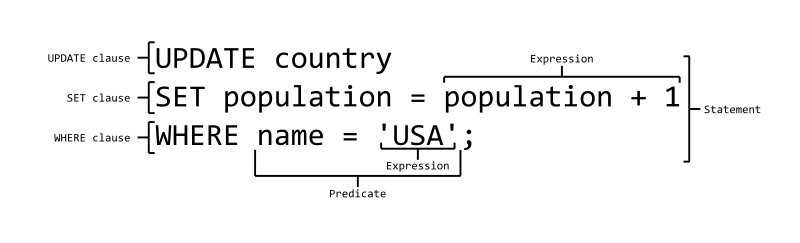
\includegraphics[keepaspectratio,width=0.5\paperwidth]{Pictures/SQL_ANATOMY_wiki.svg.png}
    \end{center}
    \caption{SQL language elements}
    \label{fig:SQL lan elem}
\end{figure}

某些数据库强制要求语句后有分号。

\subsection{真值逻辑}

空值(关键字NULL),关系数据库中对数据属性未知或缺失的一种标识。数据库表主键的取值不能为空值。在SQL的Where条件式去判断字段是否为Null时,where id = null 是无法正确执行的,必须写成 where id is null。

三值逻辑:true, false, unknown。false AND unknown为false,true OR unknown为true。与null比较运算的结果是unknown.

SQL provides two Null-specific comparison predicates: IS NULL and IS NOT NULL test whether data is or is not Null.There is also the "<row value expression> IS DISTINCT FROM <row value expression>" infixed comparison operator which returns TRUE unless both operands are equal or both are NULL. Likewise, IS NOT DISTINCT FROM is defined as "NOT (<row value expression> IS DISTINCT FROM <row value expression>)".


\subsection{ANSI SQL数据类型}
\begin{itemize}
   \item 
 CHARACTER(n) or CHAR(n): fixed-width n-character string, padded with spaces as needed
   \item 
CHARACTER VARYING(n) or VARCHAR(n): variable-width string with a maximum size of n characters
   \item 
NATIONAL CHARACTER(n) or NCHAR(n): fixed width string supporting an international character set
   \item 
NATIONAL CHARACTER VARYING(n) or NVARCHAR(n): variable-width NCHAR string
   \item 
BIT(n): an array of n bits
   \item 
BIT VARYING(n): an array of up to n bits
   \item 
INTEGER and SMALLINT
   \item 
FLOAT, REAL and DOUBLE PRECISION
   \item 
NUMERIC(precision, scale) or DECIMAL(precision, scale),precision为有效数字位数,scale为小数位数
   \item 
DATE: for date values (e.g. 2011-05-03)
   \item 
TIME: for time values (e.g. 15:51:36). The granularity of the time value is usually a tick (100 nanoseconds).
   \item 
TIME WITH TIME ZONE or TIMETZ: the same as TIME, but including details about the time zone in question.
   \item 
TIMESTAMP: This is a DATE and a TIME put together in one variable (e.g. 2011-05-03 15:51:36).
   \item 
TIMESTAMP WITH TIME ZONE or TIMESTAMPTZ: the same as TIMESTAMP, but including details about the time zone in question.
\end{itemize}





\subsection{关键词}
关键词 DISTINCT 用于返回唯一不同的值。
\begin{verbatim}
SELECT DISTINCT 列名称 FROM 表名称
\end{verbatim}


IN 操作符允许我们在 WHERE 子句中规定多个值。

\begin{verbatim}
SELECT column_name(s)
FROM table_name
WHERE column_name IN (value1,value2,...)
\end{verbatim}

操作符 BETWEEN ... AND 会选取介于两个值之间的数据范围。这些值可以是数值、文本或者日期。然而区间的开闭性因厂商而异。

\begin{verbatim}
SELECT column_name(s)
FROM table_name
WHERE column_name
BETWEEN value1 AND value2
\end{verbatim}

通过使用AS,可以为列名称和表名称指定别名(Alias)。

\begin{verbatim}
SELECT column_name(s)
FROM table_name
AS alias_name
\end{verbatim}

TOP 子句用于规定要返回的记录的数目。并非所有的数据库系统都支持 TOP 子句。
SQL Server 的语法: 
\begin{verbatim}
SELECT TOP number|percent column_name(s)
FROM table_name
\end{verbatim}

MySQL 语法:
\begin{verbatim}
SELECT column_name(s)
FROM table_name
LIMIT number
\end{verbatim}

Oracle 语法:
\begin{verbatim}
SELECT column_name(s)
FROM table_name
WHERE ROWNUM <= number
\end{verbatim}

合计函数 (比如 SUM) 常常需要添加 GROUP BY 语句.
\begin{verbatim}
SELECT column_name, aggregate_function(column_name)
FROM table_name
WHERE column_name operator value
GROUP BY column_name
\end{verbatim}

在 SQL 中增加 HAVING 子句原因是,WHERE 关键字无法与合计函数一起使用。

我们希望查找订单总金额少于 2000 的客户。
我们使用如下 SQL 语句:
\begin{verbatim}
SELECT Customer,SUM(OrderPrice) FROM Orders
GROUP BY Customer
HAVING SUM(OrderPrice)<2000
\end{verbatim}


\subsection{连接join}

内连接包含分: 相等连接,自然连接,和交叉连接.

\begin{verbatim}
SELECT *
FROM   employee 
INNER JOIN department 
ON employee.DepartmentID = department.DepartmentID
\end{verbatim}

\begin{verbatim}
SELECT *  
FROM   employee,department 
WHERE  employee.DepartmentID = department.DepartmentID
\end{verbatim}

相等连接 (equi-join,或 equijoin),是比较连接(θ连接)的一种特例,它的连接谓词只用了相等比较。使用其他比较操作符(如 <)的不是相等连接。

自然连接比相等连接的进一步特例化。两表做自然连接时,两表中的所有名称相同的列都将被比较,这是隐式的。自然连接得到的结果表中,两表中名称相同的列只出现一次.

\begin{verbatim}
SELECT *
FROM   employee NATURAL JOIN department
\end{verbatim}


交叉连接(cross join),又称笛卡尔连接(cartesian join)或叉乘(Product),它是所有类型的内连接的基础。把表视为行记录的集合,交叉连接即返回这两个集合的笛卡尔积。这其实等价于内连接的链接条件为"永真",或连接条件不存在.如果 A 和 B 是两个集合,它们的交叉连接就记为: A × B.用于交叉连接的 SQL 代码在 FROM 列出表名,但并不包含任何过滤的连接谓词.
显式的交叉连接实例:

\begin{verbatim}
SELECT *
FROM   employee CROSS JOIN department
\end{verbatim}

隐式的交叉连接实例:

\begin{verbatim}
SELECT *
FROM   employee,department;
\end{verbatim}

外连接并不要求连接的两表的每一条记录在对方表中都一条匹配的记录. 连接表保留所有记录 -- 甚至这条记录没有匹配的记录也要保留. 外连接可依据连接表保留左表, 右表或全部表的行而进一步分为左外连接, 右外连接和全连接.在标准的 SQL 语言中, 外连接没有隐式的连接符号.

左外连接(left outer join), 亦简称为左连接(left join), 若 A 和 B 两表进行左外连接, 那么结果表中将包含"左表"(即表 A)的所有记录, 即使那些记录在"右表" B 没有符合连接条件的匹配. 这意味着即使 ON 语句在 B 中的匹配项是0条, 连接操作还是会返回一条记录, 只不过这条记录的中来自于 B 的每一列的值都为 NULL. 这意味着左外连接会返回左表的所有记录和右表中匹配记录的组合(如果右表中无匹配记录, 来自于右表的所有列的值设为 NULL). 如果左表的一行在右表中存在多个匹配行, 那么左表的行会复制和右表匹配行一样的数量, 并进行组合生成连接结果.

全连接是左右外连接的并集. 连接表包含被连接的表的所有记录, 如果缺少匹配的记录, 即以 NULL 填充.一些数据库系统(如 MySQL)并不直接支持全连接, 但它们可以通过左右外连接的并集(union)来模拟实现.

自连接就是和自身连接.

\begin{verbatim}
SELECT F.EmployeeID, F.LastName, S.EmployeeID, S.LastName, F.Country
FROM Employee F, Employee S
WHERE F.Country = S.Country
AND F.EmployeeID < S.EmployeeID
ORDER BY F.EmployeeID, S.EmployeeID
-- 雇员表 Employee
\end{verbatim}

\subsection{举例}

\begin{lstlisting}[language=SQL]
SELECT *
 FROM Book
 WHERE price > 100.00
 ORDER BY title;
\end{verbatim}


 SELECT * FROM Persons
WHERE City LIKE 'N%'
--从"Persons" 表中选取居住在以 "N" 开始的城市里的人
--提示:"%" 可用于定义通配符(模式中缺少的字母)。


SELECT Book.title AS Title,
 COUNT(*) AS Authors
 FROM Book JOIN Book_author
 ON Book.isbn = Book_author.isbn
 GROUP BY Book.title;

SELECT * FROM Persons
WHERE LastName IN ('Adams','Carter')

SELECT * FROM Persons
WHERE LastName
BETWEEN 'Adams' AND 'Carter'

SELECT title,
 COUNT(*) AS Authors
 FROM Book NATURAL JOIN Book_author
 GROUP BY title;

SELECT isbn,
 title,
 price,
 price * 0.06 AS sales_tax
 FROM Book
 WHERE price > 100.00
 ORDER BY title;

SELECT isbn, title, price
 FROM Book
 WHERE price < (SELECT AVG(price) FROM Book)
 ORDER BY title;

INSERT INTO My_table
 (field1, field2, field3)
 VALUES
 ('test', 'N', NULL);

UPDATE My_table
 SET field1 = 'updated value'
 WHERE field2 = 'N';

DELETE FROM My_table
 WHERE field2 = 'N';

START TRANSACTION;
 UPDATE Account SET amount=amount-200 WHERE account_number=1234;
 UPDATE Account SET amount=amount+200 WHERE account_number=2345;
 
IF ERRORS=0 COMMIT;
IF ERRORS<>0 ROLLBACK;

CREATE TABLE tbl_1(id INT);
 INSERT INTO tbl_1(id) VALUES(1);
 INSERT INTO tbl_1(id) VALUES(2);
COMMIT;
 UPDATE tbl_1 SET id=200 WHERE id=1;
SAVEPOINT id_1upd;
 UPDATE tbl_1 SET id=1000 WHERE id=2;
ROLLBACK TO id_1upd;
 SELECT id FROM tbl_1;

CREATE TABLE My_table(
 my_field1 INT,
 my_field2 VARCHAR(50),
 my_field3 DATE NOT NULL,
 PRIMARY KEY (my_field1, my_field2)
);


ALTER TABLE My_table ADD my_field4 NUMBER(3) NOT NULL;

TRUNCATE TABLE My_table;--清零

DROP TABLE My_table;--删除

GRANT SELECT, UPDATE
 ON My_table
 TO some_user, another_user;
 
REVOKE SELECT, UPDATE
 ON My_table
 FROM some_user, another_user;



SELECT CASE WHEN i IS NULL THEN 'Null Result'  
-- This will be returned when i is NULL
            WHEN     i = 0 THEN 'Zero'         
-- This will be returned when i = 0
            WHEN     i = 1 THEN 'One'          
-- This will be returned when i = 1
            END
FROM t;


GRANT SELECT, UPDATE
 ON My_table
  TO some_user, another_user;
   
  REVOKE SELECT, UPDATE
   ON My_table
    FROM some_user, another_user;


    CREATE TABLE employees (
    id            INTEGER      PRIMARY KEY,
    first_name    VARCHAR(50)  NULL,
    last_name     VARCHAR(75)  NOT NULL,
    dateofbirth   DATE         NULL
    );   
\end{lstlisting}



\part{系统操作}
\chapter{Linux Desktop}
\section{Ubuntu/Deepin安装后的配置}

\subsection{配置网络和locale}
直接使用图形工具network-manager-gnome即可。

\subsection{硬盘设置}
设置/etc/fstab,使得一些硬盘分区开机自动挂载。
\begin{shellcmd}
UUID=4C0E	/media/D \	
ntfs-3g	defaults,nosuid,nodev,locale=zh_CN.UTF-8	0	0
UUID=077  /media/E12	ext4	defaults	0	0
\end{shellcmd}
有个图形工具叫做pysdm;另外对于ntfs分区,可以使用ntfs-config工具。
配置完/etc/fstab后,使用mount -a命令执行该文件。

\subsection{软件安装}
设置软件更新源,更新系统,并安装软件。对于deepin官方源,直接支持IPV6。对于USTC等其他源,可能需要将地址中的mirror改为mirror6。另外如果sources.list.d目录下有无法访问的地址,需要将其删除,可以将该目录重命名。

PPA清单:
\begin{verbatim}
UbuntuTweak
ppa:tualatrix/ppa
pidgin的WebQQ插件
ppa:lainme/lwqq
\end{verbatim}

包清单:
vim, vim-gnome, vim-scripts, vim-doc, vim-latexsuite,ntfs-config,pysdm,ubuntu-tweak(ppa:tualatrix/ppa),gnome-tweak-tool,nautilus-open-terminal,gdebi,Pidgin,chromium-browser, aMSN, sshpass, lcrt, texlive, texlive-xetex

需要手动下载的商用软件:
永中Office,Adobe Reader, Nutstore, Mendeley, Chrome

\subsubsection{系统工具}
Gnome桌面:gnome-shell和经典桌面gnome-panel。gnome-shell可以安装panel-dock插件。通过PPA可以安装cinnamon桌面,是LinuxMint开发的Gnome2风格的桌面。

Deb包管理器gdebi。

系统设置工具:ubuntu-tweak(ppa:tualatrix/ppa),gnome-tweak-tool。

nautilus辅助:nautilus-open-terminal

深度软件中心:deepin-softwarecenter(ppa:noobslab/deepin-sc)。

Adobe Air:官网下载安装即可。在Ubuntu12.04上安装会出错,可以执行:
\begin{verbatim}
sudo ln -s /usr/lib/i386-linux-gnu/\
libgnome-keyring.so.0.2.0 \
/usr/lib/libgnome-keyring.so.0
\end{verbatim}

\subsubsection{网络通信}
Pidgin,chromium-browser, aMSN, sshpass, lcrt, 网盘等。

\subsubsection{音视频播放}
视频播放器:Gnome-Mplayer和VLC。

视频网站客户端:ppstream。

音乐播放器:可选择banshee,audacious,rhythmbox。

歌词搜索程序:osdlyrics(ppa:osd-lyrics/ppa)为独立程序。执行osdlyrics命令,以将其打开。Ctrl+Shift+L快捷键使其解除锁定。

\subsubsection{办公软件}

VIM:vim-scripts,vim-latexsuite和vim-doc包含了Vim的一些有用插件。vim-addon-manager为Vim插件管理程序,安装该工具之后可以用vim-addons命令激活各种插件。

Latex:在texlive和texlive-xetex, texlive-latex-extra。

办公套件:永中2012青春版。

PDF文件阅读与编辑:acrobat, xournal, pdfmod。 

文献管理:mendeleydesktop。

制图工具:QtiPlot(仿制Origin), dia(模仿Visio)。论文制图也可使用办公套件中的电子表格程序,或GNUplot。 

词典: Goldendict

编程相关: ctags, cscope, doxygen, manpages-dev(Ubuntu可能已经预装), qtcreator, python-qt4, python-qt4-doc

\subsubsection{虚拟机}
KVM虚拟系统:qemu-kvm libvirt-bin virt-manager bridge-utils。
KVM制作的虚拟机保存路径一般是/var/lib/libvirt/images。
打开virt-manager可能需要root权限。


\subsection{系统设置工具一览}

系统设置:gnome-control-center

高级设置:gnome-tweak-tool

系统配置机制:gnome3用Gsettings机制取代了gconf机制。用gsettings取代了gconftool-2工具。dconf-editor是gsettings的众多后端工具之一。

\subsection{设置unity白名单}
如果是Unity桌面,设置unity白名单:
\begin{shellcmd}
gsettings set com.canonical.Unity.Panel systray-whitelist "['all']"
\end{shellcmd}

\subsection{字体配置}
文泉驿可能被默认安装了。安装少量Windows字体即可。如simsun,simfang,simhei,simkai
使用\verb+fc-list :lang=zh-cn+查看当前系统字体。

\subsection{主菜单配置}
使用alacarte创建的应用程序的快捷入口,创建在~/.local/share/applications目录下,并默认以 alacarte-made[-X].desktop 的格式命名,其中X是数字,用户可以随后重命名这个文件,菜单上显示的内容不会改变。而在alacarte工具中删除的快捷入口,也不会真的删除对应的 desktop 文件,而只是将对应文件中的Hide字段的值改为true。
以root权限安装的程序,其快捷入口大多创建在/usr/share/applications目录下,而以用户权限安装的程序,则只能将快捷入口创建在~/.local/share/applications目录下。

\subsection{默认程序配置}
有几个文件用于存储指定类型文件的关联程序,分别是 /etc/gnome/defaults.list, /usr/share/applications/defaults.list, /usr/share/applications/mimeinfo.cache, ~/.local/share/applications/mimeapps.list, ~/.local/share/applications/mimeinfo.cache。前面三个文件保存全局设置,后面两个保存用户设置。如果要修改某个类型文件的关联程序,可以通过直接修改这几个文件的方式实现。

\subsection{开机自启动程序}
gnome-session-properties工具,可以在主菜单->启动应用程序中找到。

\subsection{桌面启动器配置}
gnome-desktop-item-edit,可以创建或编辑.desktop类型的文件。创建名为my.desktop的启动器,执行:
\begin{verbatim}
gnome-desktop-item-edit --create-new my.desktop
\end{verbatim}










\section{系统备份}
需要备份的配置文件包括


\begin{verbatim}
/etc/hosts
/etc/fstab
/etc/lightdm/lightdm.conf

.bash*
.vimrc
.gitconfig
.ssh/*
.config/Chromium/User*
\end{verbatim}


\section{ISO镜像与光盘}
在Ubuntu下将文件夹做成iso镜像的工具叫做genisoimage(原名mkisofs)。可引导光盘加载后对相应文件夹使用genisoimage工具,会失去引导性。如欲保留引导性,可以使用dd工具对裸设备进行操作。如:

\verb+dd if=/dev/sr0 of=deepin.iso+

如需将iso烧录入光盘,可以使用Brasero工具。这很可能是Ubuntu系统自带的。

\section{制作USB启动盘}
可以使用dd命令或使用一些图形工具。在维基百科上有一个制作LiveUSB的软件列表。包括:
\begin{itemize}
  \item Fedora Liveusb-creator,在Windows或Linux下制作Fedora的LiveUSB
  \item Ubuntu Liveusb Creator(在命令为usb-creator-gtk或usb-creator-kde)
  \item LinuxLive USB Creator,在Windows上制作Linux LiveUSB
  \item Unetbootin,在Windows或Linux下制作UNIX LiveUSB,Ubuntu软件仓库有提供
\end{itemize}
我自己用优盘实际创建启动盘,在Ubuntu下使用Ubuntu Liveusb Creator制作失败了。用dd和Unetbootin制作成功。

如果使用dd命令,先umount这个USB设备,其名称可能是sdb1。但dd命令要作用与sdb而不是sdb1上。
\begin{verbatim}
dd if=linux_image.iso of=/dev/sdb
\end{verbatim}
尝试使用dd命令将Windows安装镜像做成启动盘,未能成功,U盘在启动时未能引导,依然由硬盘进行了引导。

制作完成后,需要更改BIOS设置,让USB-HDD(或其他USB设备类型)的设备启动优先级高于HDD。优盘可能被当作硬盘处理,如果是这种优盘,开机时需要在BIOS设置中更改的不是设备启动顺序,而是HDD启动优先级。在实验室电脑上DEL键进入BIOS设置。


\section{中文输入与显示问题}

\subsection{修改locale为GB18030}

\begin{verbatim}

/usr/share/i18n目录下为系统已经下载的字符集和locale定义文件。

在 /var/lib/locales/supported.d/local 添加两行:
zh_CN.GBK GBK和zh_CN.GB18030 GB18030 

执行sudo locale-gen 生成相应locale
在/etc/default/locale文件配置LANG,LC_*, LC_ALL等参数。其优先级递增。
也有说修改/etc/environment。但修改的结果都是只改变了root用户的locale。

普通用户的locale可以通过export LANG修改环境变量的方法进行修改。
但将locale编码改为GB码后会出现各种乱码,网上建议还是保留为UTF-8。

\end{verbatim}




\subsection{Evolution客户端没有附件}
Evolution发的邮件附件Foxmail不认,在 Evolution 的 [编辑] -> [首选项] -> [编写器首选项] 中
将“使用 Outlook / Gmail 的方式编码文件名” 前的复选框打上勾就可以了

\subsection{查看文件编码}
\begin{shellcmd}
file *
enca *
本地化编码 enconv *
\end{shellcmd}

\subsection{转换文件名由GBK为UTF8}
\begin{shellcmd}
convmv -r -f cp936 -t utf8 --notest --nosmart *
\end{shellcmd}

批量转换src目录下的所有文件内容由GBK到UTF8
\begin{shellcmd}
find src -type d -exec mkdir -p utf8/{} \;
find src -type f -exec iconv -f GBK -t UTF-8 {} -o utf8/{} \;
mv utf8/* src
rm -fr utf8
\end{shellcmd}

\subsection{文字大小不一致}
\begin{shellcmd}
sudo apt-get remove ttf-kochi-gothic ttf-kochi-mincho ttf-unfonts ttf-unfonts-core
\end{shellcmd}

\subsection{gedit中文乱码}

 命令行指定编码,例如gedit --encoding=gbk 霜冷长河.txt 。也可以配置Gsettings参数,如:
   
   \begin{shellcmd}
    gsettings set org.gnome.gedit.preferences.encodings auto-detected 
	"['UTF-8','GB18030','GB2312','GBK','BIG5','CURRENT','UTF-16']"
    gsettings set org.gnome.gedit.preferences.encodings shown-in-menu 
	"['GB18030','UTF-8','GB2312','GBK','BIG5','CURRENT','UTF-16']"
   \end{shellcmd}  

	相关图形工具叫做dconf-editor,在dconf-tools包中

  
  


\subsection{vim字符编码}
涉及3个参数:enc,fenc,fencs.
fenc为当前文件的属性,可以对当前文件set fenc,在保存,从而设置文件的编码方式。在vimrc中设置fenc,就是设置以后写入的所有文件的编码方式。
fencs为读入文件时的编码猜测列表。enc为vim工作时的编码方式,但最终写入文件时采取的编码仍取决于fenc。
 set fencs=utf-8,gbk
 set fenc=gb18030

\subsection{PDF 文件乱码}
PDF中文乱码有两种
1.汉字显示为方块:如各种从中国知网下载的论文。网上的方法多针对此种乱码

2.汉字显示为各种欧洲字母:如我电脑中的"西游记.pdf", 基于popplar的阅读器都不能搞定,foxit4linux和Adobe Reader也都失败。永中office的pdf阅读器可以搞定。foxit for linux在2009年烂尾,目前仍为1.1版。
\begin{shellcmd}
sudo apt-get install xpdf-chinese-simplified xpdf-chinese-traditional poppler-data
\end{shellcmd}

\begin{shellcmd}
sudo gedit /etc/fonts/conf.d/49-sansserif.conf 
将倒数第四行 <string>sans-serif</string>
改为 <string>sans</string>
保存即可,重启firefox
\end{shellcmd}

\subsection{unzip中文文件名乱码}
\begin{shellcmd}
sudo apt-get install p7zip-full
export LANG=zh_CN.GBK  #临时在控制台修改环境为zh_CN.GBK,然后解压缩即可
7za e docs.zip
\end{shellcmd}

\subsection{输入法问题}
ibus跟随
\begin{shellcmd}
安装ibus-gtk即可,最好另外安装:ibus-qt4
\end{shellcmd}
输入法切换
\begin{shellcmd}
im-switch -c
\end{shellcmd}









\section{中文字体的安装使用}
\subsection{查看已安装的中文字体}
\begin{shellcmd}
fc-list :lang=zh|sort
\end{shellcmd}

\subsection{安装文泉驿字体}
在Ubuntu软件仓库中,文泉驿点阵宋体和矢量正黑体分别包含于xfonts-wqy,ttf-wqy-zenhei软件包,不过很可能已经预装。
在Fedora中,点阵宋体和矢量正黑体分别位于wqy-bitmap-fonts,wqy-zenhei-fonts

\subsection{安装文鼎字体}
在Ubuntu软件仓库中,we文鼎楷体和明体分别位于ttf-arphic-ukai,ttf-arphic-uming软件包,不过很可能已经预装。
新发布的有文鼎PL报宋二GBK

\subsection{安装Windows字体}

将simsun等字体复制到目录/usr/share/fonts/TTF

在字体所在目录执行命令:
\begin{shellcmd}
mkfontdir  生成font.dir
ttmkfdir   为ttc字体生成font.dir
mkfontscale 为simsun.ttc生成font.scale
\end{shellcmd}
生成encoding文件:
\begin{shellcmd}
sudo cp /usr/share/fonts/encodings/encodings.dir ./
\end{shellcmd}
以上命令为X.org 字体系统服务。以下命令为xft字体系统服务:
\begin{shellcmd}
sudo fc-cache -fv   刷新xft字体库
\end{shellcmd}
重启X即可。

\subsection{字体大小}
1em=16px

\subsection{字体与文件名对照}
\begin{verbatim}
方正舒体              FZSTK.TTF

方正姚体              FZYTK.TTF

微软雅黑              MSYH.TTF

微软雅黑 Bold         MSYHBD.TTF

仿宋体               simfang.ttf

黑体                 simhei.ttf

楷体                 simkai.ttf

隶书                 SIMLI.TTF

宋体 & 新宋体        simsun.ttc

幼园                 SIMYOU.TTF

华文彩云            STCAIYUN.TTF

华文仿宋            STFANGSO.TTF

华文琥珀            STHUPO.TTF

华文楷体            STKAITI.TTF

华文隶书            STLITI.TTF

华文宋体            STSONG.TTF

华文细黑            STXIHEI.TTF

华文行楷            STXINGKA.TTF

华文新魏            STXINWEI.TTF

华文中宋            STZHONGS.TTF

宋体-方正超大字符集 SURSONG.TTF
\end{verbatim}
\section{LinuxDeepin 12.06源地址}

\begin{verbatim}

#北京交通大学
deb http://mirror.bjtu.edu.cn/deepin/ precise main non-free
deb-src http://mirror.bjtu.edu.cn/deepin/ precise main non-free

deb http://mirror.bjtu.edu.cn/deepin/ oneiric-updates main non-free
deb-src http://mirror.bjtu.edu.cn/deepin/ oneiric-updates main non-free

#中国科技大学
deb http://mirrors.ustc.edu.cn/deepin/ precise main non-free
deb-src http://mirrors.ustc.edu.cn/deepin/ precise main non-free

deb http://mirrors.ustc.edu.cn/deepin/ precise-updates main non-free
deb-src http://mirrors.ustc.edu.cn/deepin/ precise-updates main non-free

#清华大学
deb http://mirrors.tuna.tsinghua.edu.cn/deepin/ precise main non-free
deb-src http://mirrors.tuna.tsinghua.edu.cn/deepin/ precise main non-free

deb http://mirrors.tuna.tsinghua.edu.cn/deepin/ oneiric-updates main non-free
deb-src http://mirrors.tuna.tsinghua.edu.cn/deepin/ oneiric-updates main non-free


#天津大学(仅IPv4)
deb http://mirror.tju.edu.cn/deepin/ precise main non-free
deb-src http://mirror.tju.edu.cn/deepin/ precise main non-free

deb http://mirror.tju.edu.cn/deepin/ precise-updates main non-free
deb-src http://mirror.tju.edu.cn/deepin/ precise-updates main non-free

#天津大学ftp(仅IPv4)不用
deb ftp://mirror.tju.edu.cn/deepin/ precise main non-free
deb-src ftp://mirror.tju.edu.cn/deepin/ precise main non-free

deb ftp://mirror.tju.edu.cn/deepin/ precise-updates main non-free
deb-src ftp://mirror.tju.edu.cn/deepin/ precise-updates main non-free

#天津大学ftp(IPv4/IPv6)
deb http://jx.tju.zyrj.org/deepin/ precise main non-free
deb-src http://jx.tju.zyrj.org/deepin/ precise main non-free

deb http://jx.tju.zyrj.org/deepin/ precise-updates main non-free
deb-src http://jx.tju.zyrj.org/deepin/ precise-updates main non-free
\end{verbatim}


\section{常见错误与异常}

更新源下载目录时,提示没有与主机相关联的地址,可能是网络不通

系统死机时,如键盘还有效,可以执行CtrlAlt+f切换到其他tty,然后通过top和kill杀死一些占用资源较大的进程。如果键盘无效,应尝试安全重启。即按住Alt+SysRq,然后依此执行R,E,I,S,U,B等6个命令。

lightDM登录失败,输入用户密码执行登录崩溃又回到登录页面。通过删除~目录下Xauthority文件或许可以解决。网上其他解决方法包括:安装gdm取代lightDM,或放弃当前用户新建用户。甚至有人干脆提出重装系统。


dpkg备份出错,参\ref{err:dpkgConfig}。


\section{软件界面的绿豆沙色背景}
关于绿豆沙色的定义网上找到了多种:
1.RGB(204,232,207),RGB hex(CCE8CF)。

2.RGB hex(CCE8CF)

3.RGB(199,237,204),HSL(85,123,205)

4.HSL(84,91,205)

5.HSL(85,90,205),RGB(187,247,197)

网上有人推荐第5种.

能设置背景颜色的软件包括gnome-terminal, chromium浏览器,Adobe reader, okular等。


Adobe:Edit->Preferences->Accessibility(这里一般译作"辅助功能")->Document Color Options

okular:setting->configure okular->accessibility0->color mode

evince不能设置任意背景色,只能反色为黑背景。其他Linux上的pdf阅读器,如xournal,永中pdf阅读器等,不能设置不背景色。wine过的cajviewer,foxit reader能够设置背景色。



Chromium:
修改配置文件:
~/.config/chromium/Default/User StyleSheets/Custom.css
添加:
\begin{shellcmd}
html, body {background-color: #CCE8CC!important;}
\end{shellcmd}



关于HSL,包括:
H:Hue,色相,色调
S:Sat,Saturation,饱和度
L:Lum,Lightness,也有说Intensity,亮度

也有HSB(HSV)色彩空间,
V(Value)B(Brightness)译作明度
Adobe的软件使用HSV而非HSL
\newpage
\section{Fedora16安装之后}
\subsection{配置网络}
使用图形界面配置即可。注意netmask为24,不是255.255.255.0
\subsection{配置时间和地区}
应该设置地区为上海,这样在安装很多应用程序到时候会下载中文语言
\subsection{配置更新源}
\subsubsection{手动选择源}
开源镜像网站http://mirrors.163.com/和http://mirrors.sohu.com/下载fedora的源配置文件。为了区别镜像,打开下载的镜像文件后把三个中括号[]中的fedora分别替换为fedora-163与fedora-sohu。将修改好的配置文件保存到/etc/yum.repos.d/目录下。最后在终端输入:
\begin{shellcmd}
sudo yum makecache
\end{shellcmd}

\subsubsection{安装fastest-mirror}
\begin{shellcmd}
sudo yum -y install yum-plugin-fastestmirror 
\end{shellcmd}
\subsubsection{添加rpmfusion源}
\begin{shellcmd}
sudo rpm -ivh http://download1.rpmfusion.org/free/fedora/rpmfusion-free-release-stable.noarch.rpm 
http://download1.rpmfusion.org/nonfree/fedora/rpmfusion-nonfree-release-stable.noarch.rpm
\end{shellcmd}

\subsection{升级系统}
\begin{shellcmd}
sudo yum update
\end{shellcmd}

\subsection{配置字体}
安装文泉驿字体
\begin{shellcmd}
sudo yum -y install wqy-bitmap-fonts wqy-zenhei-fonts wqy-unibit-fonts
\end{shellcmd}
安装Windows字体
\begin{itemize}
\item 将windows字体拷贝到/usr/share/fonts/某目录/下
\item chmod 755 *
\item mkfontscale;mkfontdir;fc-cache -fv
\end{itemize}

\subsection{安装系统工具}
\subsubsection{安装gnome-tweak-tool}
\begin{shellcmd}
sudo yum -y install gnome-tweak-tool
\end{shellcmd}
\subsubsection{安装gnome shell extension}
访问https://extensions.gnome.org/
\subsubsection{其他工具}
\begin{itemize}
\item xkill.需安装xkill或xorg-x11-apps
\item nautilus-open-terminal.安装完成后ctr+alt+backspace重启X
\item faenza-icon-theme.
sudo yum -y install faenza-icon-theme
\end{itemize}

\subsection{安装常用软件}
\subsubsection{安装google-chrome}
google并没有直接提供yum源,而是以sh文件的方式提供。那么就下载这个文件
\begin{shellcmd}
wget https://dl-ssl.google.com/linux/google-repo-setup.sh

sudo sh google-repo-setup.sh 

sudo yum -y install google-chrome-stable

rm google-repo-setup.sh 
\end{shellcmd}
\subsubsection{安装latex和xelatex}
\begin{shellcmd}
sudo yum -y install texlive texlive-xetex

fmtutil --enablefmt xelatex

sudo yum -y install texmaker
\end{shellcmd}
\subsubsection{安装多媒体解码器}
fedora默认没有安装视频解码器,所以不能听歌看视频,打开歌曲时会提示缺少MPEG-1 Layer3。
首先确保系统已经安装rpmfusion源,在终端中输入命令:
\begin{shellcmd}
sudo yum -y install ffmpeg ffmpeg-libs gstreamer-ffmpeg \
libmatrosca xvidcore libdvdread libdvdnav lsdvd
sudo yum -y install gstreamer-plugins-good \ 
gstreamer-plugins-bad gstreamer-plugins-ugly
\end{shellcmd}

\subsubsection{安装Office}
安装LibreOffice:
\begin{shellcmd}
sudo yum -y groupinstall "Office/Productivity"
sudo yum -y install libreoffice-langpack-zh-Hans
\end{shellcmd}
永中Office可以从官网下载

\subsubsection{Vim及其插件}
安装gvim
\begin{shellcmd}
sudo yum -y install gvim
\end{shellcmd}
安装vim-latex
\begin{shellcmd}
sudo yum -y install vim-latex
\end{shellcmd}
所谓vim-addon-manager有两个意思,一个指debian下的软件,一个是vim插件,这里指后者.从官网下载该插件后,解压,然后配置.vimrc文件指定vim-addon-manager路径和想安装的插件的名称.
例如:
\begin{shellcmd}
set runtimepath+=/PATH/TO/VIM-ADDON-MANAGER
call vam#ActivateAddons([``vim-haxe'',``snipmate''])
call vam#ActivateAddons([``OmniCppComplete''])
call vam#ActivateAddons([``The_NERD_Commenter''])
\end{shellcmd}
下一次打开vim的时候会自动提示安装相应插件.如果插件名称有微小的错误(typo),可能会得到正确提示.

\subsubsection{KVM虚拟机}
安装KVM虚拟机
\begin{shellcmd}
sudo yum -y install kvm qemu libvirt virt-manager
\end{shellcmd}
可以利用virt-manager安装Windows XP系统,然后安装360安全卫士,搜狗拼音,360浏览器,360压缩等.注意yunio不支持ie系统的浏览器,所以可以再安装一个chrome浏览器.

\subsubsection{其他}
mendeley,yozo office,fcitx输入法,unrar解压软件,qt-creator(在ubuntu下叫做qtcreator),AdobeReader\_chs,antiword

\subsection{卸载不需要的软件}
ibus等

\subsection{修改默认应用程序}
在Fedora下,有两个配置文件:
/usr/share/applications/defauts.list \\
/usr/local/share/applications/defauts.list
其关系不明

\subsection{配置硬盘自动挂载}
修改/etc/fstab

\subsection{关闭SELinux}
修改/etc/selinux/config



\newpage




\section{Grub与系统登录}
\subsection{修改Grub配置}
配置/etc/default/grub文件,然后运行update-grub,会自动生成/boot/grub/grub.cfg文件
\subsection{安装Grub}
如果安装了多个Linux系统,最后一个安装的系统的GRUB会覆盖之前安装的GRUB。如果这不是所希望的,可以进入心目中的默认系统重新安装GRUB。如果最后安装的是Windows,
则GRUB会被破坏,不会在开机时显示GRUB界面,也需要设法进入Linux后重新安装GRUB。
进入所希望的Linux系统后,执行grub-install. grub-install copies GRUB images into /boot/grub, and uses grub-setup to install grub into the boot sector.
\begin{verbatim}
sudo grub-install /dev/sda
\end{verbatim}
可以添加选项,\verb+boot-directory=DIR+
install GRUB images under the directory DIR/grub instead of the /boot/grub directory。
如果是从LiveCD进入的系统,执行grub-install前先chroot。
如果没有LiveCD,在进入系统前停留在了如下界面上:
\begin{verbatim}
GRUB loading
error:unknow filesystem
grub rescue>
\end{verbatim}
可以执行ls命令,找到Linux被安装在了哪个分区。如果确定了分区,比如,(hd0,5),则执行\verb+ls (hd0, 5)+时会看到许多mod文件。
安装normal.mod:
\begin{verbatim}
grub rescue>set root=(hd0,5)
grub rescue>set prefix=(hd0,5)/boot/grub
grub rescue>insmod /boot/grub/normal.mod
\end{verbatim}
执行normal命令,可以恢复Grub界面。进入Linux后重新安装GRUB即可。


\subsection{登陆密码恢复}
方法如下:

1、重新启动,按ESC键进入Boot Menu,选择recovery mode(一般是第二个选项)。

2、在\#号提示符下用cat /etc/shadow,看看用户名。

3、输入passwd "用户名"(引号要有的哦)。

4、输入新的密码.

5、重新启动,用新密码登录。 
\section{lightdm登录配置}
配置文件在\verb+/etc/lightdm/+目录下,修改lightdm.conf文件
\begin{verbatim}
[SeatDefaults]
greeter-session=unity-greeter
user-session=ubuntu
greeter-show-manual-login=true #手工输入登陆系统的用户名和密码
allow-guest=false   #不允许guest登录
\end{verbatim}


\section{主机网络配置}
\subsection{配置IP地址和DNS}
可以使用图形工具network-manager-gnome.重启网络:系统设置-网络-关闭
\begin{shellcmd}
sudo vi /etc/network/interfaces 
\end{shellcmd}
\begin{verbatim}
auto lo
iface lo inet loopback
auto eth0 eth0:1
iface eth0 inet static
address 210.75.225.165
netmask 255.255.255.0
gateway 210.75.225.254
dns-nameservers 159.226.59.158 159.226.8.6
iface eth0:1 inet static
address 192.168.1.224
netmask 255.255.255.0
gateway 192.168.1.1
\end{verbatim}

新系统版本不希望手动更改/etc/resolv.conf文件,重启后会重置。修改/etc/resolvconf/tail文件,然后执行/etc/init.d/resolveconf restart,会自动生成/etc/resolve.conf文件。或者在上述/etc/network/interfaces添加dns-nameservers配置。

对于旧版系统,编辑/etc/resolv.conf文件,加入2行: 
\begin{verbatim}
nameserver 159.226.59.158
nameserver 159.226.8.6
\end{verbatim}
其他的DNS服务器包括:
谷歌:8.8.8.8
中国科大:202.38.64.1。


重启网络
\begin{shellcmd}
sudo /etc/init.d/networking restart
或者 sudo ifdown -a;sudo ifup -a;
\end{shellcmd}
如果配置了interfaces文件,那么network-manager-gnome无用,可以卸载

\subsection{代理设置}
使用tsocks这个软件。配置文件在/etc/tsocks.conf,修改local使其包含202.38.95.110。
其他工具还包括proxychains





\section{工作打印机配置}
首先确保能够连接打印机所在网络:192.168.192.0/24

\subsection{Windows XP下连接打印机}

“通过驱动连接打印机”的方式,打印机IP为:192.168.192.1。我不太明白这句话的意思。通过SMB方式连接打印机,在XP系统开始菜单,选择“添加打印机”,地址为:
\begin{verbatim}
//192.168.192.235/3nmedia_tzb_printer
\end{verbatim}

\subsection{Gnome桌面连接打印机}
网上的帖子大多是通过系统设置->打印机方式获得添加打印机的界面,但Linux Deepin 12.06下该界面无法解锁。使用另一套工具:system-config-printer-gnome软件包,该软件包包含了system-config-printer.py程序,执行它,就得到了一个添加打印机的界面。该程序由/usr/bin/system-config-printer调用。

执行system-config-printer命令后,选择以SMB方式添加打印机,等待程序搜索SMB网络,可以找到上述打印机。需要安装驱动程序,可以在给出的列表中选择Laser 1015驱动。



\section{Ubuntu快捷键}

Gnome快捷键参考系统设置->键盘->快捷键,其他应用的快捷键以该应用的具体设置为准。

\subsection{Gnome}

显示桌面:Ctrl+Alt+D 或者 Super+D,Ctrl+Super+D

前往其他工作区:Ctrl+Alt+Arrowkey

切换同一程序的不同窗口 :Alt+`

移动到其他工作区 :Ctrl+Alt+Shift+Arrowkey

打开帮助:F1

打开主菜单:Alt+F1

启动程序:Alt+F2

全屏 :F11

锁屏:Ctrl+Alt+L

注销:Ctrl+Alt+Del

\subsection{General Frame Window}

关闭Tab Ctrl+W

关闭Frame Alt+F4

恢复Frame原始大小  Alt+F5

最小化 Alt+F9

最大化 Alt+F10

\subsection{Nautilus}

显示隐藏的内容 : Ctrl+H

将路径从按钮变成文字 :  Ctrl+L(如需恢复回按钮,点击文字,按Esc)


\subsection{Terminal}

(Add a shift to normal operation)

清屏: Ctrl + L

暂停并置之后台: Ctrl+Z(fg to recover),may be a SIGTSTP signal,SUSP character

发送SIGQUIT信号: Ctrl + \

冻结终端显示: Ctrl + S(Ctrl+Q to recover,maybe a SIGCONT),NOT a SIGSTOP

向上滚屏一行:Ctrl+Shift+UpArrow

向上滚动一屏:Shift+PageUp

向上滚动至顶:Shift+Home


\subsection{tty切换}
Ctrl+Alt+F1~F6 从X切换到tty1~tty6

Ctrl+Alt+F7 返回X视窗系统











\section{软件包安装与管理}

一般而言,aptitude命令优于apt命令。

查看已经安装了哪些包:
\begin{verbatim}
dpkg -l
\end{verbatim}

查看软件包版本和其他信息
\begin{verbatim}
 aptitude show mendeleydesktop
 apt-cache showpkg mendeleydesktop (详细信息,包括依赖关系)
 apt-cache show mendeleydesktop (概要信息)
 apt-cache depends xxx
 apt-cache rdepends xxx(被依赖)
\end{verbatim}

搜索软件包:
\begin{verbatim}
 aptitude search pkgname (推荐)
apt-cache search 正则表达式
\end{verbatim}

如果官方源中没有相关的包,可以查看PPA仓库:
\url{https://launchpad.net/ubuntu/+ppas}

安装ppa软件的一般方法有两种:
\begin{verbatim}
sudo add-apt-repository source_line
sudo add-apt-repository ppa:<user>/<ppa-name>
\end{verbatim}

\begin{verbatim}
查找文件属于哪个包
apt-file search/find filename
查询软件包包含的文件
atp-file list/show pkgname
\end{verbatim}

编译时缺少h文件的自动处理
\begin{verbatim}
sudo auto-apt run ./configure
\end{verbatim}

清理下载包的临时存放目录/var/cache/apt/archives
\begin{verbatim}
apt-get clean
apt-get autoclean (只删除部分无用的包)
\end{verbatim}

备份当前系统安装的所有包的列表
\begin{verbatim}
dpkg --get-selections | grep -v deinstall > ~/somefile
\end{verbatim}

从上面备份的安装包的列表文件恢复所有包
\begin{verbatim}
dpkg --set-selections < ~/somefile
sudo dselect
\end{verbatim}

删除系统不再使用的孤立软件
\begin{verbatim}
sudo apt-get autoremove
\end{verbatim}

查看包在服务器上面的地址
\begin{verbatim}
apt-get -qq --print-uris install ssh | cut -d\' -f2
\end{verbatim}

除所有已删除包的残馀配置文件
\begin{verbatim}
dpkg -l |grep ^rc|awk '{print $2}' |sudo xargs dpkg -P 
\end{verbatim}
如果你的系统中没有残留配置文件了,会报错。

\subsection{dpkg出错}
\label{err:dpkgConfig}
\begin{verbatim}
dpkg:处理 xxx (--configure)时出错
\end{verbatim}
处理方式,找到/var/lib/dpkg/info目录,备份他处,重新目录,执行
\begin{verbatim}
apt-get update
apt-get -f install
\end{verbatim}
在将新建的info目录同备份的目录合并





















\section{网络对时}
\begin{shellcmd}
date -s 20110813
ntpdate 210.72.145.44
\end{shellcmd}

国家授时中心的NTP服务器地址:210.72.145.44
教育网的ntp:
\begin{verbatim}
s1a.time.edu.cn 北京邮电大学
s1b.time.edu.cn 清华大学
s1c.time.edu.cn 北京大学
 s1d.time.edu.cn 东南大学
 s1e.time.edu.cn 清华大学
 s2a.time.edu.cn 清华大学
 s2b.time.edu.cn 清华大学
 s2c.time.edu.cn 北京邮电大学
s2d.time.edu.cn 西南地区网络中心
s2e.time.edu.cn 西北地区网络中心
s2f.time.edu.cn 东北地区网络中心
 s2g.time.edu.cn 华东南地区网络中心
 s2h.time.edu.cn 四川大学网络管理中心
 s2j.time.edu.cn 大连理工大学网络中心
 s2k.time.edu.cn CERNET桂林主节点
 s2m.time.edu.cn 北京大学
\end{verbatim}

\chapter{RSPE相关操作}
\section{ACTA-8000启动}
\subsection{CPUA启动}
串口线连接到RSPE的COM-A上。执行reboot命令重启RSPE,当它进入UBoot后输入Ctrl+C,使其停留在UBoot命令行界面。
下载Linux镜像:
\begin{shellcmd}
tftpboot 0 vmlinux.64.iscsi.order
\end{shellcmd}

其中,vmlinux.64.iscsi.order是Linux镜像(Linux内核需要在编译时选择支持crc32c),目前已经被预先放置在文件服务器的usr/local/nginx/html目录下。
如果上述过程不成功,需要确保物理连接畅通,同时SPI6被设置为UBoot默认端口,且SPI6地址和文件服务器在同一网段内:
\begin{shellcmd}
setenv ethact spi6
setenv ipaddr 192.168.10.224
\end{shellcmd}

下载镜像成功后,加载镜像:
\begin{shellcmd}
bootoctlinux 0 coremask=0xffff mem=0
\end{shellcmd}

coremask对应16个CPU的掩码,0xffff表示16个CPU全部加载,mem后为内存大小(MB),mem=0表示全部内存。
进入linux后,配置IP:
\begin{shellcmd}
ifconfig spi6 192.168.10.224
ifconfig spi7 192.168.0.224
\end{shellcmd}

从文件服务器下载iscsi相关软件包(目前已经被预先放置在文件服务器)并解压:
\begin{shellcmd}
tftp -g -r iscsi.tar.gz 192.168.10.233
tar xzvf iscsi.tar.gz
cd iscsi
chmod +x *
\end{shellcmd}

\section{设置bootcmd}
\begin{verbatim}
setenv bootcmd tftpboot 0 p\;bootoct 0 coremask=0xff
\end{verbatim}
\section{OCTEON模拟器环境下的GDB调试}
需要两个终端。

终端1:
\begin{verbatim}
oct-sim $(TARGET) -quiet -noperf -numcores=2 -uart1=2021 -debug
\end{verbatim}


终端2:
\begin{verbatim}
 mipsisa64-octeon-elf-gdb -x gdbfile_pc 
\end{verbatim}
上述gdbfile\_pc的内容为:

\begin{verbatim}
file pushtest
set spawn-sim off
target octeon tcp::2021
b main
set step-all on
c
\end{verbatim}

然后就可以正常调试了。

\section{OCTEON服务器登录}

\subsection{ACTA-7200登录}
使用telnet登陆7220后执行oct-serial 2命令登陆CPU-B。Ctrl+A+C退出CPU-B。dpbreset 2重启CPU-B。

运行文件服务器上的hello程序:
\begin{shellcmd}
tftpboot 0 hello
bootoct 0 coremask=*** stack=*** heap=***
\end{shellcmd}

\subsection{Hili登录}
DRM组目前有两台Hili,分别登录194和130服务器,在root权限下使用minicom登录。

\begin{verbatim}
minicom configuration A
minicom configuration B
\end{verbatim}

上述命令分别登录CPA-A和CPU-B
\section{OCTEON-SDK的使用}

\subsection{安装SDK}
\begin{shellcmd}
rpm –i /media/cdrom/*.rpm
/media/cdrom/patch_1.7
\end{shellcmd}
如果SVN中已经安装了SDK,可通过如下命令安装到用户目录下
\begin{shellcmd}
svn checkout http://192.168.1.199/svn/OCTEON-SDK/branches/2012-03-27/
\end{shellcmd}

\subsection{设置环境变量}
执行env-setup脚本会设置环境变量:
\begin{shellcmd}
source env-setup OCTEON_CN58XX
\end{shellcmd}
上述命令需要每次开机时重新执行.如需自动执行,Cavium幻灯片上有如下说明:
Add the following 3 lines to your ~/.bash\_profile and log out/in:
\begin{shellcmd}
pushd /usr/local/Cavium_Networks/OCTEON-SDK
source env-setup OCTEON_CN38XX
popd
\end{shellcmd}


\subsection{查看SDK版本}
查看executive/cvmx-version.h文件内容即可。

\section{开机运行}
\subsection{CPUA启动}
串口线连接到RSPE的COM-A上。执行reboot命令重启RSPE,当它进入UBoot后输入Ctrl+C,使其停留在UBoot命令行界面。
下载Linux镜像:
\begin{shellcmd}
tftpboot 0 vmlinux.64.iscsi.order
\end{shellcmd}

其中,vmlinux.64.iscsi.order是Linux镜像(Linux内核需要在编译时选择支持crc32c),目前已经被预先放置在文件服务器的usr/local/nginx/html目录下。
如果上述过程不成功,需要确保物理连接畅通,同时SPI6被设置为UBoot默认端口,且SPI6地址和文件服务器在同一网段内:
\begin{shellcmd}
setenv ethact spi6
setenv ipaddr 192.168.10.224
\end{shellcmd}

下载镜像成功后,加载镜像:
\begin{shellcmd}
bootoctlinux 0 coremask=0xffff mem=0
\end{shellcmd}

coremask对应16个CPU的掩码,0xffff表示16个CPU全部加载,mem后为内存大小(MB),mem=0表示全部内存。
进入linux后,配置IP:
\begin{shellcmd}
ifconfig spi6 192.168.10.224
ifconfig spi7 192.168.0.224
\end{shellcmd}

从文件服务器下载iscsi相关软件包(目前已经被预先放置在文件服务器)并解压:
\begin{shellcmd}
tftp -g -r iscsi.tar.gz 192.168.10.233
tar xzvf iscsi.tar.gz
cd iscsi
chmod +x *
\end{shellcmd}

\section{SE程序设计与编译}
\subsection{资源配置}
Static configuration of the hardware resources are controlled by the include file "cvmx-config.h". This file is generated from the executive-config.h file and other files in the config directory of the application. 
Example: creating an application that uses simple executive
\begin{shellcmd}
% mkdir application
% cd application
% mkdir config
% cp $OCTEON_ROOT/executive/executive-config.h.template config/executive-config.h
\end{shellcmd}
(then edit config/executive-config.h to tune the flags/settings as appropriate for the application)
\section{IP-SAN连接}
加载iscsi相关模块:
\begin{shellcmd}
modprobe crc32c;
insmod iomtr_kstat.ko;
insmod scsi_transport_iscsi_dxf.ko;
insmod libiscsi_dxf.ko;
insmod iscsi_tcp_dxf.ko;
echo "127.0.0.1       localhost.localdomain   localhost" > /etc/host;
mkdir /var/lock/;
\end{shellcmd}

配置initiator端id,即IQN。主机的IQN必须经过磁盘阵列客户端的“定义”。
\begin{shellcmd}
mkdir /etc/iscsi;
echo "InitiatorName=iqn.2002-10.com.infortrend:raid.sn7905538.309" > /etc/iscsi/initiatorname.iscsi;
\end{shellcmd}

启动iscsi守护进程
\begin{shellcmd}
./iscsid_dxf;
\end{shellcmd}

寻找远程磁盘。在解压出的iscsi目录下,执行
\begin{shellcmd}
./iscsiadm_dxf -m discovery -t sendtargets -p 192.168.0.17;
\end{shellcmd}

该IP下的磁盘记录信息会被获取到本地。如果需要(如磁盘连接异常需重新连接),可用以下命令清空记录:
\begin{shellcmd}
./iscsiadm_dxf -m node -o delete
\end{shellcmd}

获取盘阵信息后,进行iscsi登录,连接磁盘:
\begin{shellcmd}
./iscsiadm_dxf -m node  -p 192.168.0.17 -l;
\end{shellcmd}

查看磁盘挂载情况:
\begin{shellcmd}
fdisk -l;
\end{shellcmd}

获取iscsi会话信息
\begin{shellcmd}
./iscsiadm_dxf -m session -P3
\end{shellcmd}




\section{运行时系统信息识别}

\subsection{processor\_id}
cvmx.h中定义了\verb+cvmx_get_proc_id+函数。所谓processor\_id,应该是用于标示处理器的型号。例如有cvmx.h中有如下代码:
\begin{verbatim}
 return (cvmx_get_proc_id() == OCTEON_CN38XX_PASS1);
\end{verbatim}


\subsection{OCTEON MODEL识别}
使用\verb|OCTEON_IS_MODEL(x)|宏可判断是否为模型x。该宏和x可取的值定义在executive/octeon\_model.h中。

\subsection{是否为模拟器}
\begin{verbatim}
cvmx_sysinfo_get() 返回值的board_type字段代表“板子”类型,其取值由enum cvmx_board_types_enum定义。对于模拟器,取CVMX_BOARD_TYPE_SIM。
\end{verbatim}



\chapter{Linux服务器}
\section{磁盘速率测量}
关于磁盘负载的生成器,主要有iometer和dd。

对于速率测量,在ubuntu下需要安装sysstat软件包,它提供了iostat工具。另外ubuntu下也有sar工具。
\section{资源消耗查询}
\begin{shellcmd}
 df -h:磁盘分区使用率
 du -h:文件夹大小
 tree -h:文件夹和文件大小,树形打印
 free -m:内存使用率
 vmstat -s M:虚拟内存占用情况
\end{shellcmd}
上述free命令中,m选项设置单位为MB。因为buffer和cache是否算作已用空间有争议,故分两种算法列出。
 上述vmstat命令,M表示单位为MB,如果是m,则为1000*1000B

如果只想查看当前目录下所有子目录的大小,有
\begin{shellcmd}
du -s
\end{shellcmd}
或者
\begin{shellcmd}
du -h --max-depth=1
\end{shellcmd}

对于top命令,最重要的两个交互快捷键是h和q,分别打印帮助信息和退出top。利用好h命令就能够进行各种复杂操作。例如,F可以选择一个field列,以其为标准进行行排序,如n表示MEM。可以查出Ubuntu占用内存最剧烈的是chromium-browser等浏览器。
 




\section{dstat工具}
iostat, vmstat, ifstat 三合一的工具,用来查看系统性能。
你可以这样使用:

\begin{verbatim}
alias dstat='dstat -cdlmnpsy'
\end{verbatim}


\section{环境变量}
Linux系统里的env命令可以显示当前用户的环境变量,还可以用来在指定环境变量下执行其他命令。下面来比较一下set,env和export命令的异同:set命令显示当前shell的变量,包括当前用户的变量;env命令显示当前用户的变量;export命令显示当前导出成用户变量的shell变量。每个shell有自己特有的变量(set)显示的变量,这个和用户变量是不同的,当前用户变量和你用什么shell无关,不管你用什么shell都在,比如HOME,SHELL等这些变量,但shell自己的变量不同shell是不同的,比如BASH\_ARGC,BASH等,这些变量只有set才会显示,是bash特有的,export不加参数的时候,显示哪些变量被导出成了用户变量,因为一个shell自己的变量可以通过export “导出”变成一个用户变量。

\section{文件查找工具}
locate, find, whereis, which等
\section{主机硬件与OS信息查询}
\subsection*{查询主机名称}
hostname命令可以查询主机名称。但是很多主机的名称都取作localhost
\subsection*{Linux内核版本}
\begin{shellcmd}
cat /proc/version:查询内核信息
uname -r:查询Linux内核版本号
uname -a:查询内核信息
\end{shellcmd}
注意不要用file命令通过查看可执行文件的信息来判断当前主机的内核版本号,二者关系复杂
\subsection*{Linux发行版信息}
\begin{shellcmd}
lsb_release -a 
cat /etc/issue
cat /etc/redhat-release
rpm -q redhat-release:查看Redhat release号
\end{shellcmd}
Redhat release号和实际的版本之间存在一定的对应关系:
\begin{verbatim}
   redhat-release-3AS-1 -> Redhat Enterprise Linux AS 3
   redhat-release-3AS-7.4 -> Redhat Enterprise Linux AS 3 Update 4
   redhat-release-4AS-2 -> Redhat Enterprise Linux AS 4
   redhat-release-4AS-2.4 -> Redhat Enterprise Linux AS 4 Update 1
   redhat-release-4AS-3 -> Redhat Enterprise Linux AS 4 Update 2
   redhat-release-4AS-4.1 -> Redhat Enterprise Linux AS 4 Update 3
   redhat-release-4AS-5.5 -> Redhat Enterprise Linux AS 4 Update 4 
\end{verbatim} 

\subsection*{查看字长:32/64位}
\begin{shellcmd}
getconf LONG_BIT
getconf WORD_BIT
file /bin/ls
lsb_release -a
\end{shellcmd}
\subsection*{CPU信息}
\subsubsection*{CPU架构}
arch命令或uname -m:结果如"i386", "i486","i586", "alpha", "sparc", "arm", "m68k", 
"mips", "ppc","ia64","x86\_64"等;ia64和x86\_64就说明这台机器是64位的
\subsubsection*{CPU详细信息}
\begin{shellcmd}
cat /proc/cpuinfo
\end{shellcmd}
\subsubsection*{CPU数与核数}
Linux下可以在/proc/cpuinfo中看到每个cpu的详细信息。但是对于双核的cpu,在cpuinfo中会看到两个cpu。常常会让人误以为是两个单核的cpu。
其实应该通过Physical Processor ID来区分单核和双核。而Physical Processor ID可以从cpuinfo或者dmesg中找到.
flags如果有ht说明支持超线程技术。判断物理CPU的个数可以查看physical id 的值,相同则为同一个物理CPU。
\begin{shellcmd}
 cat /proc/cpuinfo |grep "model name" && cat /proc/cpuinfo |grep "physical id"
\end{shellcmd}
\subsubsection*{CPU型号}
\begin{shellcmd}
cat /proc/cpuinfo |grep "model name"
\end{shellcmd}

\subsection*{内存信息}
\begin{shellcmd}
cat /proc/meminfo |grep MemTotal
sudo dmidecode |grep -A16 "Memory Device$"
\end{shellcmd}

\subsection*{硬盘大小}
\begin{shellcmd}
fdisk -l |grep Disk
\end{shellcmd}
df命令主要用来查询文件系统信息,可以用来查看硬盘以挂载的分区的大小
\begin{shellcmd}
df -h
\end{shellcmd}

\subsection*{主板型号}
\begin{shellcmd}
sudo dmidecode |grep -A16 "System Information$"
cat /proc/pci
\end{shellcmd}













\section{日志信息}


\subsection{查看用户连接信息}
连接时间日志一般由/var/log/wtmp和/var/run/utmp这两个文件记录,不过这两个文件都无法使用tail或cat命令直接查看。该文件由系统自动更新。Linux提供了如 w, who, finger, id, last, lastlog,ac等命令读取这部分的信息。
\begin{description}
    \item[finger]user information lookup program.用户详细信息,甚至包括电话号码。 
    \item[w]Show who is logged on and what they are doing.
    \item[last]show listing of last logged in users.\verb+last|grep reboot+记录了开机时间。 
    \item[lastlog] reports the most recent login of all users or of a given user
    \item[users]print the user names of users currently logged in to the current host. 其实就是第一列。
    \item[ac]ac应是accounting的缩写。打印用户连接时间的总和,指多个pty
    \item[id]当前用户的id和组id
    \item[uptime]查看开机时间,其实就是w输出的第一行
\end{description}

The utmp file allows one to discover information about who is currently using the system. 

The  wtmp  file records all logins and logouts.

\subsection{命令历史记录}


.bash\_history 记录了Bash命令历史,但不包含最近执行的命令。

/var/log/apt/目录下的文件记录了apt相关的命令执行历史。

\subsection{进程清算(accounting)}

acct是一个系统调用:

\begin{verbatim}
 #include <unistd.h>
 int acct(const char *filename);
\end{verbatim}

The  acct()  system  call  enables  or  disables process accounting.  If called with the name of an existing file as its argument,
accounting is turned on, and records for each terminating process are appended to filename as it terminates.  An argument of  NULL
causes accounting to be turned off.

例如:
\verb+ acct("/var/log/pacct");+

accton为系统命令,清算一段时间内终结的进程, 记录于清算文件中, 默认为/var/log/account/pacct。lastcomm用来读取清算文件。
\verb+ accton [OPTION] on|off|filename+

例如:
\begin{verbatim}
sudo accton somefile
sudo accton off
lastcomm -f somefile
\end{verbatim}

默认的pacct清算似乎早已默认开启,使得\verb+sudo accton on+命令显得多余。


\subsection{内核日志}
dmesg: 显示内核信息

\subsection{系统与服务日志}
由syslog的服务管理,比如下面的日志文件都是由syslog日志服务驱动的:      
/var/log/lastlog :记录最后一次用户成功登陆的时间、登陆IP等信息 

/var/log/messages :记录Linux操作系统常见的系统和服务错误信息 

/var/log/secure :Linux系统安全日志,记录用户和工作组变坏情况、用户登陆认证情况 

/var/log/btmp :记录Linux登陆失败的用户、时间以及远程IP地址 

/var/log/cron :记录crond计划任务服务执行情况

syslog服务由配置文件/etc/syslog.conf或/etc/rsyslog.conf.

/etc/syslog.conf的内容格式为:
\verb+消息类型.错误级别    动作域+

\subsection{日志转储}
Linux中使用logrotate命令进行日志转储。可以配合cron计划任务轻松实现日志文件的定时转储, /etc/logrotate.conf提供了日志转储的相关配置.
包括发送电子邮件。















\section{Minicom}

\subsection{Minicom配置}

创建或编辑配置文件,保存为/etc/minirc.Filename或/etc/minicom/minirc.Filename,因系统而异。
\begin{lstlisting}[language=bash]
minicom -s Filename
\end{lstlisting}
配置文件指定设备名、波特率等。Dell服务器的串口设备名为/dev/ttyS0, 4个USB接口的设备名为/dev/ttyUSB0-/dev/ttyUSB3。对于Hili的串口连接,要求码率为115200, 软、硬件流控制都设置为No。

配置文件格式如下:
\begin{lstlisting}
    # Machine-generated file - use ``minicom -s'' to change parameters. 
     pr port             /dev/ttyUSB0 
     pu baudrate         115200 
     pu bits             8 
     pu parity           N 
     pu stopbits         1 
     pu rtscts           No
\end{lstlisting}

\subsection{Minicom登录}
按照指定配置文件,登录串口设备:
\begin{lstlisting}[language=bash]
minicom Filename
\end{lstlisting}

minirc.dfl指定了默认配置,minicom命令不加任何参数时安装该文件进行初始化。

登录后ctrl+a z显示各种快捷键选项,ctrl+a x退出并reset,ctrl+a q退出不reset。

ssh远程登录并登录minicom,执行:
\begin{lstlisting}[language=bash]
ssh -t HOSTNAME minicom Filename
\end{lstlisting}

\section{RHEL网络配置}


是否启用网络、主机名称信息于/etc/sysconfig/network文件中配置。
\begin{verbatim}
NETWORKING=yes
HOSTNAME=localhost.localdomain //修改该值作为主机名,如:rhel.lpwr.net
\end{verbatim}

配置网卡IP等信息, 编辑指定网络接口配置文件
\begin{verbatim}
/etc/sysconfig/network-script/目录下建立形如ifcfg-eth0:0的文件进行配置

DEVICE=eth0 //指定接口名称
ONBOOT=yes //系统启动时加载
BOOTPROTO=static //IP地址静态配置,若该值为“dhcp”则为动态获得
IPADDR=192.168.0.1 //设置IP地址
NETMASK=255.255.255.0 //设置子网掩码
GATEWAY=192.168.0.254 //设置默认网关
\end{verbatim}

重启网络以执行配置更新:

\begin{verbatim}
/etc/init.d/network restart
\end{verbatim}

DNS信息由/etc/resolv.conf配置
\begin{verbatim}
127.0.0.1 localhost.localdomain localhost //该行强烈建议保留
192.168.0.1 rhel.lpwr.net rhel //必须有三个字段:IP、FQDN、HOSTNAME
\end{verbatim}



\section{网络连接故障原因}
\begin{itemize}
    \item 物理上是否连通
        \begin{itemize}
            \item 网线、电口模块是否受损
            \item 如果多条网线直连,是否两个端一一对应
            \item 如果走交换机,交换机是否正常
            \item 有时Hili某些网口不通,reset之后也不行。需要断电才可以。

        \end{itemize}
    \item 配置是否正确
        \begin{itemize}
            \item 是否属于同一子网
            \item IP是否冲突
            \item (Hili)MAC地址是否冲突
        \end{itemize}
    \item 软件是否正常
        曾遇到Dell服务器不能ping通时,将该网口用ifconfig重启后即可用。
        
\end{itemize}

另外,不能确定某服务器是否正常时,将两台相同的服务器连接到同一个交换机内,配置为同一个子网。Hili只能ping通其中一台,说明另一台有问题。
\section{分区创建与挂载}

\subsection{分区查看与创建}
分区创建可使用fdisk和cfdisk命令,fdisk的man页自称buggy,推荐使用cfdisk等。
df可以查看分区使用率。

\subsection{分区格式化}
使用mkfs工具。

\subsection{分区挂载}
例如挂载优盘sdc,执行:
\begin{verbatim}
sudo mount -t msdos -o uid=li,gid=li /dev/sdc1 /mnt
\end{verbatim}


\section{进程查看与控制}

按照NOHUP方式执行进程:
\begin{verbatim}
nohup ./cdn > /dev/null 2>&1 &
\end{verbatim}
noup:run a command immune to hangups, with output to a non-tty

\subsection{进程查找}
\begin{verbatim}
pgrep [-u user] pattern
如 pgrep -u root evince
pstree -p
-p选项会打印出PID的值,否则只打印名字
ps -ef
\end{verbatim}

\subsection{单一进程查看}
ps, top
\begin{verbatim}
ps pid
top [-p pid]
\end{verbatim}


\subsection{信号发送}
\begin{verbatim}
kill [信号] pid
pkill [信号] pattern
\end{verbatim}

\subsection{X下杀死进程}
xkill杀死单一窗口
如需重启,可按住Alt SysRq,再依次按REISUB



\section{RHEL配置yum}

\begin{enumerate}
    \item 如果没有安装yum,先安装yum
    \item /etc/yum.repos.d目录下,删除原有的repo文件,替换为Centos的源文件
    \item /etc/yum.conf文件,添加一行\verb+timeout=120+,未验证必要性
    \item 使用rpm命令import选项导入密钥文件
    \item 运行yum update命令
\end{enumerate}

关于密钥文件,目前不是很懂其原理。网上提到的有:
\begin{verbatim}
http://ftp.sjtu.edu.cn/centos/5/os/i386/RPM-GPG-KEY-CentOS-5
http://centos.ustc.edu.cn/centos/RPM-GPG-KEY-CentOS-5
\end{verbatim}
如果不导入密钥,那么安装可能不能成功。yum有nogpgcheck选项,以及配置文件也有相关选项,可能会强制安装软件。未测试。

安装软件包时需要知道这个包在yum系统中的名字。使用yum search命令。例如,需要安装git时,键入
\begin{verbatim}
yum search git
\end{verbatim}
易知git在yum系统中可能叫做git.i386.

\section{SSH便捷登录}

\subsection{登录后执行命令}
ssh命令后追加shell命令使得后者在目标主机执行后在本地打印,然后关闭ssh连接。如果需要保留在目标主机上,可以使用-t选项,并追加bash命令。
\begin{lstlisting}[language=bash]
   ssh HOSTNAME -t ``cd /somedir; bash'' 
\end{lstlisting}

\subsection{ssh免输密码}

默认情况下ssh命令的每次执行都需要输入密码以进行验证。scp命令基于ssh,也需要密码。有两种方法能够避免在使用ssh和scp时输入密码。

\subsubsection{sshpass}
sshpass工具可用于保存ssh密码。在ssh和scp命令前添加\verb+sshpass -p <password>+即可。

\subsubsection{服务器端保存客户机公钥}
首先,客户端需要生成自身的公钥和私钥,使用ssh-keygen命令,公私钥文件在生成后保存到客户机~/.ssh目录下。
\begin{verbatim}
ssh-keygen -t rsa
\end{verbatim}

其次,将公钥文件追加到服务器主机\verb+~/.ssh/authorized_keys+文件结尾。该文件模式需为600,.ssh目录需为700。
\begin{verbatim}
client> scp <pubkey_file> root@server_host:~
server> cat <pubkey_file> >> /root/.ssh/authorized_keys
server> chmod 700 /root
server> chmod 700 /root/.ssh
server> chmod 600 /root/.ssh/authorized_keys
\end{verbatim}
经实验,root家目录访问权限也可以为750, .ssh权限也可以为755, authorized\_keys权限也可为644。
Ubuntu上传客户端公钥的方法也可以是:
\begin{verbatim}
ssh-copy-id -i ~/.ssh/id_rsa.pub root@serverhost
\end{verbatim}


然后,按正常方式进行ssh登录。此时输入密码。以后则无需输入密码了。

\section{sshd服务启动}
在Ubuntu上,临时启动、停止和查看一个服务可以执行:
\begin{verbatim}
service ssh start/stop/status
/etc/init.d/ssh start/stop/status
\end{verbatim}

如果希望开机时不自动启动sshd,只有需要用时才开启sshd,目前找到的办法是:破坏\verb+/etc/init/ssh.conf+文件,如将其重命名,或将exec语言破坏。
这样,sshd将脱离service命令的管理。需要临时开启时,执行
\begin{verbatim}
/usr/sbin/sshd 或者
/usr/sbin/sshd -D
\end{verbatim}

如果遇到一个错误:
\begin{verbatim}
Missing privilege separation directory: /var/run/sshd
\end{verbatim}

只需执行:
\begin{verbatim}
mkdir -p /var/run/sshd
\end{verbatim}





\section{Ubuntu系统服务}

Ubuntu使用service命令来临时启动和停止服务。service是一个脚本,调用start,stop等可执行文件。

Ubuntu上可以使用工具update-rc.d或sysv-rc-conf来管理服务,但经尝试似乎效果不理想。


\section{RHEL系统服务}
service命令运行\verb+/etc/init.d+目录下的System V脚本或\verb+/etc/init+目录下的upstart jobs。这些脚本应至少支持start, stop参数,有些支持status, restart参数。

service runs a System V init script or upstart job in as predictable environment as possible, removing most environment variables and with current working directory set to \verb+/+.  

重启网络:
\begin{verbatim}
service network restart
\end{verbatim}

查看所有服务的状态
\begin{verbatim}
service --status-all
将所有支持status命令的服务运行一遍
\end{verbatim}

\section{tftp服务器端安装}
Ubuntu下,安装tftp-hpa。在/etc/default/tftp-hpa目录下配置。
RHEL下,安装tftp-server。/etc/xinetd.d/tftp配置。守护进程名称为in.tftpd。
\section{用户与组}

\subsection{用户增加与删除}
useradd, adduser, userdel, deluser, usermod, delgroup

使用ueradd时,如果后面不添加任何参数选项,例如:\verb+#sudo useradd test+创建出来的用户将是默认“三无”用户:一无Home Directory,二无密码,三无系统Shell。
使用adduser时,创建用户的过程更像是一种人机对话,系统会提示你输入各种信息,然后会根据这些信息帮你创建新用户。
\begin{verbatim}
useradd -m -s /bin/bash user 
-m表示创建家目录,默认不创建。
注意-p选项以密文方式设置密码,似乎没什么用。
userdel -r user
删除用户及其家目录
\end{verbatim}

\subsection{设置用户为sudoer}
执行visudo命令,在打开的文件中添加一行
\begin{verbatim}
userA ALL=(ALL)  ALL
userB ALL=(ALL)  NOPASSWD: ALL
\end{verbatim}
visudo相当于修改/etc/sudoers文件。userB执行sudo的时候不需要输入密码。

可以在bashrc或profile中添加如下内容,修改PATH
\begin{verbatim}
PATH=/usr/sbin:/usr/local/sbin:/sbin:$PATH
export PATH
\end{verbatim}

\subsection{查看用户所在组}
方法一:id命令
方法二:/etc/group,格式:
\begin{verbatim}
group_name:password('x'):GID:user_list(separated by commas)
\end{verbatim}

/etc/passwd包含了家目录,shell等用户信息

\subsection{用户的shell}
查看系统安装的shell
\begin{verbatim}
cat /etc/shells
\end{verbatim}

查看当前shell
\begin{verbatim}
echo $SHELL
\end{verbatim}

更改某用户的shell
\begin{verbatim}
usermod -s /bin/zsh someuser
\end{verbatim}


\subsection{修改用户名和主机名}
用户名在/etc/shadow中修改,主机名需要在/etc目录下hostname和hosts两个文件下修改

\subsection{用户密码}
只能使用passwd命令。在创建用户后创建密码。


\part{桌面应用操作}

\chapter{Latex与办公套件}

\section{Latex中文环境安装}
\label{sec:LatexInstall}.
\subsection{基于CJK宏包的方法}
Debian下相关软件包:
texlive texlive-latex-extra latex-cjk-chinese
参\ref{sec:zhCJK}。
CJK 作为一个 LaTeX2e 宏包,其对字体的定义遵照 NFSS(新字体选择框架)。Dpkg环境只提供了gbsn,gkai两种简体中文字体。可以使用一些网上流传的工具(如gbkfonts)将ttl字体转换为CJK宏包需要的PK字体,很繁琐,勿尝试。

\subsection{基于xeCJK宏包的方法}
Debian下相关软件包:
texlive texlive-latex-extra texlive-xetex

xeCJK的好处就是能够直接使用系统安装的字体。

\subsection{CTEX}
Ubuntu原生软件包系统不提供对CTEX的安装,只能到网上下载相关文件,复制到目录\verb+/usr/share/texmf-texlive/tex/latex/ctex/fontset+下,然后执行sudo texhash命令。

字体配置路径可能是
\begin{verbatim}
/usr/local/texlive/tex/latex/ctex/fontset/
\end{verbatim}
相关文件包括: ctex-xecjk-winfonts.def

\subsection{从CTAN安装texlive}
\url{http://oss.ustc.edu.cn/CTAN/systems/texlive}

\url{http://mirrors.tuna.tsinghua.edu.cn/CTAN/systems/texlive}

\subsection{背景知识}
texhash又叫mktexlsr,用于刷新ls-R文件名数据库。

CTAN全称是Comprehensive Tex Archive Network.The TeX Archive Network is a set of fully-mirrored ftp sites providing the most complete, up-to-date TeX-related software possible.





\section{格式调整技巧}
\subsection{description换行}
需要hfill命令,否则编译失败。
\begin{verbatim}
\begin{description}
    \item[First] \hfill \\
        The first item
    \item[Second] \hfill \\
        The second item
    \item[Third] \hfill \\
        The third etc \ldots
\end{description}
\end{verbatim}

\subsection{下划线的处理}
章节标题的下划线会出错,应该转义。url,字体名称中的下划线不会出错,即便vim给出警告也是如此。
\section{查看帮助}
texdoc打开pdf格式的文档说明。
\begin{verbatim}
texdoc xetex
texdoc listings
\end{verbatim}





\subsection{Latex转rtf格式}
\begin{verbatim}
latex2rtf -C utf8 filename
\end{verbatim}
其中,filename不包含tex后缀。

公式错乱的话,可以用-M4选项将单行公式变成图片,或-M12将单行和文内公式全部变bitmap图片.转换成bitmap的过程非常耗时。

\subsection{Latex转html}
\begin{verbatim}
latex2html -html_version 4.0,latin1,unicode -split +0 haha
\end{verbatim}
其中,3.0以上的版本才能正确转换utf8编码的中文,split +0表示生成一个单一的html文件,否则会生成一堆文件。

\subsection{Latex公式转LibreOffice公式}
LibreOffice可安装Texmaths插件,即可以Latex的方式输入公式。


\subsection{LibreOffice转Latex}
安装Debian包libreoffice-writer2后,latexLibreOffice自动获得writer2latex扩展。可以以tex格式导出文件。但LibreOffice中的中文不能正确处理,会以[16进制数字串?]的方式写入tex文件。可以用perl或python等将这种串转为utf8编码,参\ref{subsec:PythonUnicode}。



\section{插入内容}

\subsection{插入图片}
graphicx宏包:
\begin{verbatim}
\begin{figure}[htpb]
    \begin{center}
        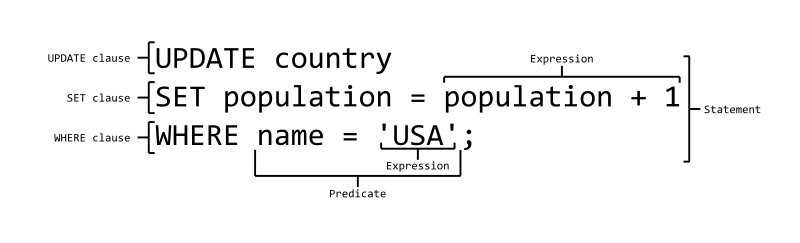
\includegraphics[keepaspectratio,width=0.8\paperwidth]{Pictures/SQL_ANATOMY_wiki.svg.png}
    \end{center}
    \caption{SQL language elements}
    \label{fig:SQL lan elem}
\end{figure}
\end{verbatim}


\subsection{插入特殊字符}
反斜杠 \verb+\textbackslash+

\subsection{URL}
示例:
\begin{verbatim}
\url{https://launchpad.net/ubuntu/+ppas}
\end{verbatim}
章节标题的下划线会出错,应该转义。url,字体名称中的下划线不会出错,即便vim给出警告也是如此

\subsection{插入交叉引用}
引用图片编号,使用ref而不是cite

\subsection{插入程序代码}
可以使用宏包listings。
示例:
\begin{verbatim}
\usepackage{listings} 

\begin{lstlisting}[language=C]
int rank()
{ 
    return 0;
}
\end{lstlisting}
\end{verbatim}


\section{OpenOffice公式输入技巧}
\begin{verbatim}
1.转义字符:即在公式中出现 OOO Math的保留字和保留符号,可以用双引号扩起来,就按照普通文本处理
2. 在odt正文中输入fn,按F3即可实现自动编号的公式,公式初始内容为E=mc^2
也可以通过插入自动图文集->公式编号来实现
实际上,fn就是一个自动图文集的缩写
\end{verbatim}
\section{Word参考文献自动修改}
写论文,参考文献的修改很麻烦,删除一个,添加一个,就需要改一长串数字。怎么办呢。本人推荐一种简单方法:尾注法。方法如下(以Word2003为例):
\begin{verbatim} 
1.光标移到要插入参考文献的地方,菜单中“插入”——“引用”-“脚注和尾注”。   
2.对话框中选择“尾注”,编号方式选“自动编号”,所在位置建议选“节的结尾”。   
3.如“自动编号”后不是阿拉伯数字,选右下角的“选项”,在编号格式中选中阿拉伯数字。   
4.确定后在该处就插入了一个上标“1”,而光标自动跳到文章最后,前面就是一个上标“1”,这就是输入第一个参考文献的地方。   
5.将文章最后的上标“1”的格式改成正常(记住是改格式,而不是将它删掉重新输入,否则参考文献以后就是移动的位置,这个序号也不会变),再在它后面输入所插入的参考文献(格式按杂志要求来慢慢输,好像没有什么办法简化)。   
6.对着参考文献前面的“1”双击,光标就回到了文章内容中插入参考文献的地方,可以继续写文章了。   
7.在下一个要插入参考文献的地方再次按以上方法插入尾注,就会出现一个“2”(Word已经自动为你排序了),继续输入所要插入的参考文献。   
8.所有文献都引用完后,你会发现在第一篇参考文献前面一条短横线(页面视图里才能看到),如果参考文献跨页了,在跨页的地方还有一条长横线,这些线无法选中,也无法删除。这是尾注的标志,但一般科技论文格式中都不能有这样的线,所以一定要把它们删除。   
9.切换到普通视图,菜单中“视图”——“脚注”,这时最下方出现了尾注的编辑栏。   
10.在尾注右边的下拉菜单中选择“尾注分隔符”,这时那条短横线出现了,选中它,删除。   
11.再在下拉菜单中选择“尾注延续分隔符”,这是那条长横线出现了,选中它,删除。   
12.切换回到页面视图,参考文献插入已经完成了。这时,无论文章如何改动,参考文献都会自动地排好序了。如果删除了,后面的参考文献也会自动消失,绝不出错。   
13.参考文献越多,这种方法的优势就体现的越大。
还没完,标号上的方括号如何加呢?很简单:
在全文中,查找尾注标记^e,然后全部替换为[^&]即可;如果用了脚注就查找脚注标记^f,再全部替换为[^&]便可以了(注意查找时让“不限定格式”按钮为灰色)
别看步骤多,操作一遍,就知道很简单了。
\end{verbatim}
\section{一次性帮你解决毕业论文的所有排版问题}
\begin{verbatim}

一、图表和公式的自动编号 
     在论文中,图表和公式要求按在章节中出现的顺序分章编号,例如图1-1,表2-1,公式3-4等。在插入或删除图、表、公式时编号的维护就成为一个大问题,比如若在第二章的第一张图(图2-1)前插入一张图,则原来的图2-1变为2-2,2-2变为2-3,…,更糟糕的是,文档中还有很多对这些编号的引用,比如“流程图见图2-1”。如果图很多,引用也很多,想象一下,手工修改这些编号是一件多么费劲的事情,而且还容易遗漏!表格和公式存在同样的问题。 
     能不能让Word对图表公式自动编号,在编号改变时自动更新文档中的相应引用?答案是肯定的!下面以图的编号为例说明具体的作法。 
     自动编号可以通过Word的“题注”功能来实现。按论文格式要求,第一章的图编号格式为“图1-×”。将图插入文档中后,选中新插入的图,在“插入”菜单选“题注”,新建一个标签“图1-”,编号格式为阿拉伯数字(如果不是点击“编号”修改),位置为所选项目下方,单击“确定”后Word就插入了一个文本框在图的下方,并插入标签文字和序号,此时可以在序号后键入说明,比如“形态学膨胀运算示例”,还可以移动文本框的位置,改动文字的对齐方式等。再次插入图时题注的添加方法相同,不同的是不用新建标签了,直接选择就可以了。Word会自动按图在文档中出现的顺序进行编号。 
     在文档中引用这些编号时,比如“如图1-1所示”,分两步做。插入题注之后,选中题注中的文字“图1-1”,在“插入”菜单选“书签”,键入书签名,点“添加”。这样就把题注文字“图1-1”做成了一个书签。在需要引用它的地方,将光标放在插入的地方(上例中是“如”字的后面),在“插入”菜单选“交叉引用”,弹出对话框中引用类型选“书签”,“引用内容”为“书签文字”,选择刚才键入的书签名后点“插入”,Word就将文字“图1-1”插入到光标所在的地方。在其他地方需要再次引用时直接插入相应书签的交叉引用就可以了,不用再做书签。 
至此我们就实现了图的编号的自动维护,当在第一张图前再插入一张图后,Word会自动把第一张图的题注“图1-1”改为“图1-2”,文档中的“图1-1”也会自动变为“图1-2”。 
     表格编号的作法与图相同,唯一不同的是表格的题注在表格上方,且要求左对齐。公式的编号略有不同,插入公式后,将公式单独放在一个段落,版式为“嵌入式”(Word默认),光标放在公式之后,不要(注意是“不要”)选中公式,在“插入”菜单选“题注”,由于没有选中项目,所以“位置”一项为灰色,新建标签“公式1-”,点击“插入”,Word就将标签文字和自动产生的序号插入到光标所在位置。在文档中引用公式编号的方法与图相同,此处不在赘述。公式的编号要求在右边行末,具体的方法在“制表位的使用”一节详细说明。 
     这里顺便说一下,交叉引用、书签和题注都是Word的域。域是文档中可能发生变化的内容,Word使用域来进行文档自动化。多个域的联合使用可以实现更复杂的功能,各个域的具体使用方法请参考Word的帮助。 
注: 
    题注中新建标签时,Word会自动在标签文字和序号之间加一个空格,看起来不那么舒服,可以在插入题注后将空格删除,然后再将文字做成书签。² 
书签名最好用图(表、公式)的说明文字,尽量做到见名知“图”。² 
图(表、公式)的编号改变时,文档中的引用有时不会自动更新,可以鼠标右击引用文字,在弹出的菜单中选“更新域”。关闭文档再打开Word会更新所有的域。²
 
二、制表位的使用 
     制表位是指水平标尺上的位置,它指定了文字缩进的距离或一栏文字开始的位置,使用户能够向左、向右或居中对齐文本行;或者将文本与小数字符或竖线字符对齐。用户可以在制表符前自动插入特定字符,如句号或划线等。默认情况下,按一次Tab键,Word将在文档中插入一个制表符,其间隔为0.74厘米。 
     制表位的类型包括:左对齐,居中对齐,右对齐,小数点对齐和竖线对齐等,这些制表位的使用方法大致相同,这里仅根据论文中公式排版的要求和目录的制作为例说明制表位的使用方法和效果,更详细的说明请参阅Word的帮助文档。 
     论文里的公式要求单独放在一个段落,公式居中;按章节进行编号,编号用小括号括起来放在右边行末。首先输入公式和编号,公式的版式选择“嵌入式”,编号用小括号括起来。然后把光标放在公式所在的段落里,点击页面左上角的制表位图标,切换到居中制表位,用鼠标在水平标尺上大约中间的位置点一下,这样就放置了一个居中制表位在点击的地方,如果位置不合适还可以用鼠标拖动进行调节。再把左上角的制表位图标切换到右对齐制表位,用放置居中制表位相同的方法放置一个右对齐制表位在行末。 
     设置好制表位后,把光标放在公式的前面,按一下Tab键,这样就在公式的前面插入了一个制表符,此时公式以居中制表位为中心居中对齐,再把光标移到公式和左括号之间,再按Tab键插入一个制表符,编号就跑到行末了。 
     用制表位的方法来处理公式的排版,很简单也很方便,不用去敲很多空格去把公式挪到中间,编号推到行末。还有一个好处,若公式或编号的长度发生变化时,Word会自动调节以使公式始终在页面的中间,编号始终在行末,不会因为公式或编号变长而换行。更简单的作法是把公式段落的设置保存为样式,所有的公式段落应用此样式,即简单又方便,而且可以保持所有的公式段落制表位的一致。手工设置制表位,你能保证每次居中制表位的位置都一样吗?! 
     涉及到制表位还有一个概念:前导符。前导符是填充制表符所产生的空位的符号,一般有实线、虚线、点划线等,在目录中经常见到(就是标题和页码之间的圆点)。制作目录时,敲入标题和页码后,在行末设置一个右对齐制表位。点击“格式|制表位”,制表位对话框显示了光标所在段落的制表位信息。选择右对齐制表位,前导符选择圆点(Word默认无前导符),确定后在标题和页码之间插入一个制表符,可以看到页码跑到行末了,而且页码和标题之间用圆点进行了填充。当页码或标题长度变化时,Word会自动增加或删除圆点。这里用目录做例子只是想说明前导符的使用方法,其实制作目录还有更好的方法,下文详述。 
注: 
    1)按一次Tab键插入的是一个制表符,因此不要在文档中用制表符代替空格来产生空白间隔。不然若把这段文字粘贴到其他存在不同制表位的段落,或文档的制表符默认设置变化时,版面就会混乱。 
    2)有时候按Tab键后Word会产生一个灰色箭头,这实际上是Word的制表符格式标记,格式标记还有段落标记(拐弯的箭头)、空格(灰色圆点)等。这些格式标记在打印文档时是不会打印出来的,格式标记是否显示以及显示哪些可以在“工具|选项”的“视图”选项卡里进行设置。

 
三、目录的制作 
     目录是用来列出文档中的各级标题及标题在文档中相对应的页码。首先介绍Word的一个概念:大纲级别。Word使用层次结构来组织文档,大纲级别就是段落所处层次的级别编号,Word提供9级大纲级别,对一般的文档来说足够使用了。Word的目录提取是基于大纲级别和段落样式的,在Normal模板中已经提供了内置的标题样式,命名为“标题1”、“标题2”,…,“标题9”,分别对应大纲级别的1-9。我们也可以不使用内置的标题样式而采用自定义样式,但有点麻烦。下文中的目录制作方法直接使用Word的内置标题样式,关于自定义样式的方法请参阅Word的帮助文档。 
     目录的制作分三步进行。 
     1)修改标题样式的格式。通常Word内置的标题样式不符合论文格式要求,需要手动修改。在菜单栏上点“格式|样式”,列表下拉框中选“所有样式”,点击相应的标题样式,然后点“更改”。可修改的内容包括字体、段落、制表位和编号等,按论文格式的要求分别修改标题1-3的格式。 
     2)在各个章节的标题段落应用相应的格式。章的标题使用“标题1”样式,节标题使用“标题2”,第三层次标题使用“标题3”。使用样式来设置标题的格式还有一个优点,就是更改标题的格式非常方便。假如要把所有一级标题的字号改为小三,只需更改“标题1”样式的格式设置,然后自动更新,所有章的标题字号都变为小三号,不用手工去一一修改,即麻烦又容易出错。关于如何应用样式和自动更新样式,请参考Word帮助。 
     3)提取目录。按论文格式要求,目录放在正文的前面。在正文前插入一新页(在第一章的标题前插入一个分页符),光标移到新页的开始,添加“目录”二字,并设置好格式。新起一段落,菜单栏选“插入|索引和目录”,点“目录”选项卡,“显示级别”为3级,其他不用改,确定后Word就自动生成目录。若有章节标题不在目录中,肯定是没有使用标题样式或使用不当,不是Word的目录生成有问题,请去相应章节检查。此后若章节标题改变,或页码发生变化,只需更新目录即可。 
注: 
   目录生成后有时目录文字会有灰色的底纹,这是Word的域底纹,打印时是不会打印出来的(如果你愿意浪费一张纸可以试着打印一下目录)。在“工具|选项”的“视图”选项卡可以设置域底纹的显示方式。²
 
四、参考文献的编号和引用 
     参考文献的标注本不是一件麻烦的事情,但是对参考文献编号后就成了一件麻烦的事情,产生的问题和图表公式编号的问题是一样的。手工维护这些编号是一件费力而且容易出错的事情,我们的目的是让Word自动维护这些编号。很幸运,它可以做到,方法跟图表公式的作法相似。光标放在引用参考文献的地方,在菜单栏上选“插入|脚注和尾注”,弹出的对话框中选择“尾注”,点击“选项”按钮修改编号格式为阿拉伯数字,位置为“文档结尾”,确定后Word就在光标的地方插入了参考文献的编号,并自动跳到文档尾部相应编号处请你键入参考文献的说明,在这里按参考文献著录表的格式添加相应文献。参考文献标注要求用中括号把编号括起来,至今我也没找到让Word自动加中括号的方法,需要手动添加中括号(补充:在全文中,查找尾注标记^e,然后全部替换为[^&]即可;如果用了脚注就查找脚注标记^f,再全部替换为[^&]便可以了(注意查找时让“不限定格式”按钮为灰色))。 
     在文档中需要多次引用同一文献时,在第一次引用此文献时需要制作尾注,再次引用此文献时点“插入|交叉引用”,“引用类型”选“尾注”,引用内容为“尾注编号(带格式)”,然后选择相应的文献,插入即可。不要以为已经搞定了,我们离成功还差一步。论文格式要求参考文献在正文之后,参考文献后还有发表论文情况说明、附录和致谢,而Word的尾注要么在文档的结尾,要么在“节”的结尾,这两种都不符合我们的要求。 
    解决的方法似乎有点笨拙。首先删除尾注文本中所有的编号(我们不需要它,因为它的格式不对),然后选中所有尾注文本(参考文献说明文本),点“插入|书签”,命名为“参考文献文本”,添加到书签中。这样就把所有的参考文献文本做成了书签。在正文后新建一页,标题为“参考文献”,并设置好格式。光标移到标题下,选“插入|交叉引用”,“引用类型”为“书签”,点“参考文献文本”后插入,这样就把参考文献文本复制了一份。选中刚刚插入的文本,按格式要求修改字体字号等,并用项目编号进行自动编号。
到这里,我们离完美还差一点点。打印文档时,尾注页同样会打印出来,而这几页是我们不需要的。当然,可以通过设置打印页码范围的方法不打印最后几页。这里有另外一种方法,如果你想多学一点东西,请接着往下看。 
     选中所有的尾注文本,点“格式|字体”,改为“隐藏文字”,切换到普通视图,选择“视图|脚注”,此时所有的尾注出现在窗口的下端,在“尾注”下拉列表框中选择“尾注分割符”,将默认的横线删除。同样的方法删除“尾注延续分割符”和“尾注延续标记”。删除页眉和页脚(包括分隔线),选择“视图|页眉和页脚”,首先删除文字,然后点击页眉页脚工具栏的“页面设置”按钮,在弹出的对话框上点“边框”,在“页面边框”选项卡,边框设置为“无”,应用范围为“本节”;“边框”选项卡的边框设置为“无”,应用范围为“段落”。切换到“页脚”,删除页码。选择“工具|选项”,在“打印”选项卡里确认不打印隐藏文字(Word默认)。 
好了,试着打印一下尾注所在的页,是不是白纸?!
 
五、页眉页脚的制作 
     首先介绍一个概念:节。这里的“节”不同于论文里的章节,但概念上是相似的。节是一段连续的文档块,同节的页面拥有同样的边距、纸型或方向、打印机纸张来源、页面边框、垂直对齐方式、页眉和页脚、分栏、页码编排、行号及脚注和尾注。如果没有插入分节符,Word默认一个文档只有一个节,所有页面都属于这个节。若想对页面设置不同的页眉页脚,必须将文档分为多个节。 
     论文里同一章的页面采用章标题作为页眉,不同章的页面页眉不同,这可以通过每一章作为一个节,每节独立设置页眉页脚的方法来实现。首先介绍页眉的制作方法。 
     在各个章节的文字都排好后,设置第一章的页眉(若连页眉都不知怎么加,请参考Word帮助)。然后跳到第一章的末尾,菜单栏上选“插入|分隔符”,分节符类型选“下一页”,不要选“连续”(除非你想第二章的标题放在第一章的文字后面而不是另起一页),若是奇偶页排版根据情况选“奇数页”或“偶数页”。这样就在光标所在的地方插入了一个分节符,分节符下面的文字属于另外一节了。光标移到第二章,这时可以看到第二章的页眉和第一章是相同的,鼠标双击页眉Word会弹出页眉页脚工具栏,工具栏上有一个“同前”按钮(图像按钮,不是文字),这个按钮按下表示本节的页眉与前一节相同,我们需要的是各章的页眉互相独立,因此把这个按钮调整为“弹起”状态,然后修改页眉为第二章的标题,完成后关闭工具栏。如法炮制制作其余各章的页眉。 
     页脚的制作方法相对比较简单。论文页面的页脚只有页码,要求从正文开始进行编号,但是,在正文前还有扉页、授权声明、中英文摘要和目录,这些页面是不需要编页码的,页码从正文第一章开始编号。首先,确认正文的第一章和目录不属于同一节。然后,光标移到第一章,点击“视图|页眉和页脚”弹出页眉页脚工具栏,切换到页脚,确保“同前”按钮处于弹起状态,插入页码,这样正文前的页面都没有页码,页码从第一章开始编号。 
注: 
页眉段落默认使用内置样式“页眉”,页脚使用“页脚”样式,页码使用内置字符样式“页码”。如页眉页脚的字体字号不符合要求,修改这些样式并自动更新即可,不用手动修改各章的页眉页脚。²论文里页眉使用章标题,可以采用章标题做成书签,然后在页眉交叉引用的方法来维护两者的一致。²
 
六、其他技巧 
分页符(Ctrl+Enter) 
     顾名思义,分页符是用来分页的,分页符后的文字将另起一页。论文中各章的标题要求新起一页,放在新页的第一行,这时就可以使用分页符。在前一章的最后放置一个分页符,这样不管前一章的版面有什么变化,后一章的标题总是出现在新的一页上。 
肯定还有人用敲多个回车的方法来把章标题推到新页!这样做的缺点是显而易见的。若前一章的版面发生了变化,比如删掉了一行,这时后一章的标题就跑到前一章的最后一页的末尾;若增加一行,则后一章标题前又多了一个空行。快抛弃这种费力不讨好的作法吧!
换行符(Shift+Enter)u 
这里又涉及Word的一个概念:段落。段落是独立的信息单位,具有自身的格式特征,如对齐方式、间距和样式。每个段落的结尾处都有段落标记(一个灰色的拐弯箭头)。敲Enter键有两个作用,一是在光标位置插入一个段落标记,表示一个段落的结束;二是另起一行。换行符和敲Enter键不同,它只有第二个作用,没有第一个,即换行符的前一行和后一行仍然属于同一个段落,共享相同的段落格式。 
双击图标 
    以一个例子作为说明。你可能需要在论文里画一个简单的流程图,你先插入了需要的文本框并加入了相应的文字,排好位置,这时你需要用箭头把这些文本框连起来,你用鼠标在绘图工具栏上点了一下箭头图标,然后画了一个箭头,再点一下图标,又画一个箭头,第三次点图标,画了第三个箭头,…有点麻烦是不是?要是可以连续画该多好!事实上可以做到!用鼠标在箭头图标上双击,然后在需要的地方画箭头,看到了吗?当画完一个箭头时,图标依然保持为嵌入状态,表示可以连续作图。当所有箭头都画完后,再在嵌入的图标上点一下,嵌入的图标弹起,Word又回到了文字输入状态。 
    不只箭头图标具有这样的功能,其他许多图标都可以如此。格式刷就是一个。当需要把一段特殊的文字格式多次应用时,双击格式刷,连续刷需要的文字,很方便。 
居中和右对齐 
你还在用插入空格的方法来把章节标题推到页面中间吗?太土了吧!用格式工具栏上的居中按钮吧。右对齐按钮会从行末开始排列文字。
\end{verbatim}
\section{xelatex下的字体调节}

\subsection{字形调节}
一般有:
\begin{verbatim}
\textrm{...} \textbf{...}
\textsf{...} \textit{...} 
\texttt{...} \textsl{...}
\emph{...} \underline{...}
\textsc{...} 
\end{verbatim}
或者\verb+\itshape \sffamily+等。


\subsection{全局字体设置}
示例:
\begin{verbatim}
\setCJKmainfont[BoldFont=SimHei,ItalicFont=KaiTi]{SimSun}
\setCJKmainfont[ItalicFont={KaiTi_GB2312}]{SimSun}
\setCJKsansfont{SimHei}
\end{verbatim}
注意,\verb+KaiTi_GB2312+中的下划线不需要转义。需要事先查看系统已经安装了的字体:
\begin{verbatim}
fc-list :lang=zh
\end{verbatim}
以下模板从网上抄得:
\begin{verbatim}
\usepackage{xeCJK}
\CJKlanguage{zh-cn}
\setmainfont{DejaVu Sans}
\setCJKmainfont{AR PL UMing CN}
\setCJKsansfont[BoldFont=AR PL New Kai]{AR PL New Kai}
\setCJKmonofont{DejaVu Sans Mono}
\setCJKfamilyfont{song}{AR PL New Sung}
\setCJKfamilyfont{kai}{AR PL New Kai}
\setCJKfamilyfont{hei}{文泉驿正黑}
\end{verbatim}

\subsection{xeCJK字体调用}
在导言中设置hei字体为系统黑体:
\begin{verbatim}
\setCJKfamilyfont{hei}{SimHei}
\end{verbatim}
在正文中使用字体调用:
\begin{verbatim}
{\CJKfamily{hei}
这里对CDN有个要求,就是对同一个媒体资源子文件,相应的transferID必须保持一致
}
\end{verbatim}






\section{中文处理的CJK方法}
\label{sec:zhCJK}

\begin{verbatim}
\documentclass{article}
\usepackage{CJKutf8}
\begin{document}
\begin{CJK}{UTF8}{gkai}
这是一个楷体中文测试,处理简体字。
\end{CJK}
\begin{CJK}{UTF8}{gbsn}
这是一个宋体中文测试,处理简体字。
\end{CJK}
\end{document}
\end{verbatim}

另一个例子:
\begin{verbatim}
\documentclass{article}
\usepackage{CJK}
\begin{document}
\begin{CJK}{UTF8}{gbsn}
\CJKfamily{gbsn}
{\Huge          万岁}
{\footnotesize  万岁}
{\scriptsize    万岁}
{\tiny          万岁}
\end{CJK}
\end{document}
\end{verbatim}


\section{论文结构中文化}
日期,日期和参考文献
\begin{shellcmd}
\renewcommand{\bibname}{\begin{center} \sffamily 参考文献 \end{center}}
\renewcommand{\today}{\number\year 年 \number\month 月 \number\day 日}
\renewcommand{\contentsname}{目录}
\end{shellcmd}



\chapter{编程工具}
\section{Cscope用法要略}

生成数据库:cscope -Rbq 
R表示递归,b表示build后不进入cscope自带的查询界面,q表示quick,加速日后的查询。

在vim下使用时应添加数据库,cs show命令显示当前已经添加的数据库,执行cs add cscope.out添加当前目录下cscope.out文件作为数据库。可以通过修改.vimrc来自动添加当前目录和父目录下的数据库。

\begin{verbatim}
"for cscope
if has("cscope")
        set csprg=/usr/bin/cscope
        set csto=0
        set cst 
        set nocsverb
        " add any database in current directory
        if filereadable("cscope.out")
                cs add cscope.out
        elseif filereadable("../cscope.out")
                cs add ../cscope.out
        elseif filereadable("../../cscope.out")
                cs add ../../cscope.out
                " else add database pointed to by environment
        elseif $CSCOPE_DB != ""
                cs add $CSCOPE_DB
        endif
        set csverb
endif

\end{verbatim}

在vim下键入:cs可以查看相关操作提示。具体用法参考见:h cscope或cscope的man页。

\begin{verbatim}
 USAGE   :cs find {querytype} {name}

            {querytype} corresponds to the actual cscope line
            interface numbers as well as default nvi commands:

                0 or s: Find this C symbol
                1 or g: Find this definition
                2 or d: Find functions called by this function
                3 or c: Find functions calling this function
                4 or t: Find this text string
                6 or e: Find this egrep pattern
                7 or f: Find this file
                8 or i: Find files #including this file

\end{verbatim}

可以在vim中添加一些键映射:

\begin{verbatim}
 nmap <F2>s :cs find s <C-R>=expand("<cword>")<CR><CR>
nmap <F2>g :cs find g <C-R>=expand("<cword>")<CR><CR>
nmap <F2>c :cs find c <C-R>=expand("<cword>")<CR><CR>
nmap <F2>t :cs find t <C-R>=expand("<cword>")<CR><CR>
nmap <F2>e :cs find e <C-R>=expand("<cword>")<CR><CR>
nmap <F2>f :cs find f <C-R>=expand("<cfile>")<CR><CR>
nmap <F2>i :cs find i ^<C-R>=expand("<cfile>")<CR>$<CR>
nmap <F2>d :cs find d <C-R>=expand("<cword>")<CR><CR>

nmap <F3>s :scs find s <C-R>=expand("<cword>")<CR><CR>
nmap <F3>g :scs find g <C-R>=expand("<cword>")<CR><CR>
nmap <F3>c :scs find c <C-R>=expand("<cword>")<CR><CR>
nmap <F3>t :scs find t <C-R>=expand("<cword>")<CR><CR>
nmap <F3>e :scs find e <C-R>=expand("<cword>")<CR><CR>
nmap <F3>f :scs find f <C-R>=expand("<cfile>")<CR><CR>
nmap <F3>i :scs find i ^<C-R>=expand("<cfile>")<CR>$<CR>
nmap <F3>d :scs find d <C-R>=expand("<cword>")<CR><CR>

\end{verbatim}









\section{Ctags关键用法}

创建元数据:
\begin{verbatim}
  ctags -R
\end{verbatim}
  对于C++,结合omnicppcomplete插件,有:
\begin{verbatim}
   ctags -R --c++-kinds=+p --fields=+iaS --extra=+q
\end{verbatim}

为vim配置tags搜索路径:
在.vimrc中添加设置。如使用绝对路径:
\begin{verbatim}
 set tags=/home/xxx/myproject/tags
\end{verbatim}

如果设置成自动搜索上级目录的tags:
\begin{verbatim}
set tags=./tags;
\end{verbatim}
注意第一行的分号表示递归向上搜索,点斜杠表示当前文件所在目录而非当前目录。

\begin{verbatim}
:set tags=./tags,./../tags,./*/tags
\end{verbatim}
使用当前目录下的tags文件, 上一级目录下
的tags文件, 以及当前目录下所有层级的子目录下的tags文件.


\begin{verbatim}
:set tags=~/proj/**/tags
\end{verbatim}
一种深度搜索目录的形式

查找:
\begin{verbatim}
vim -t tag名
:ta tag名
:tselect tag名 同名tag选择

\end{verbatim}

跳转:
\begin{verbatim}
Ctrl+]  跳转至函数定义
ctrl+O 返回
ctrl+I 前进
Ctrl+T 返回(与ctrl+])对应
:tp  同名tag,跳转到前一个
:tn  同名tag,跳转到下一个
:tfirst, :tlast 
\end{verbatim}


裂屏显示:
\begin{verbatim}
Ctrl-W ] 裂屏跳转至函数定义
[vertical] stag name 裂屏查找并跳转
\end{verbatim}



\section{数据文件分析工具}

\subsection{十六进制显示}

od, hexdump等工具将文件按照8进制、16进制、ASCII等形式打印出来。hexdiff同时打开两个文件,进行比较。

\subsection{十六进制编辑}
hexer工具能够以vi风格的界面编辑数据文件,而ghex则基于Gnome窗口系统。其他工具大多基于curses家族,包括hexedit, lfhex, dhex等。

\subsection{其他}

strings:寻找文件中的字符串。可用于分析可执行文件。
\section{Doxygen文档生成工具}
\begin{verbatim}
http://www.stack.nl/~dimitri/doxygen/index.html

http://sourceforge.net/projects/doxygen/
\end{verbatim}

\begin{shellcmd}
doxygen -g
doxygen Doxyfile
\end{shellcmd}

要点:
\begin{enumerate}
	\item 修改Doxyfile,可以指定项目名称,概要,语言(Chinese)等。Doxyfile中比较重要的字段还包括
	\begin{enumerate}
		\item OUTPUT\_LANGUAGE
		\item OPTIMIZE\_OUTPUT\_FOR\_C
		\item EXTRACT\_ALL, EXTRACT\_STATIC
	\end{enumerate}
	\item \verb+ \mainpage \author +等命令比较常用
	\item 无需学习过多内容
\end{enumerate}

在vim中安装doxygen-toolkit插件,常用命令包括
\begin{verbatim}
:Dox
生成函数注释
\end{verbatim}

\section{GDB调试器使用要略}


如果想对elfname程序进行调试,则:
\verb+gdb elfname+或\verb+gdb --args elfname arg1 arg2+\ldots
也可以只输入gdb,在交互界面上设置:
file elfname;
set args argv1 argv2 \ldots 

该程序在编译时需使用-g选项。

基本的用法,可以在进入gdb后执行help。

每次执行run,会从头开始运行程序。run简称r。

\subsection{查看源码}
list 显示当前位置10行代码。list简称l。

list funcname:显示某函数附近的10行代码

list lineno: 显示第lineno行及其上下文10行代码


\subsection{断点}
help b可以查看断电的用法。

首先需要明确,如果在第18行设置断点,指的是在第18行执行之前中止,而非之后。

设置断点:breakpoint命令,简称b,参数为[文件名:]行号或函数名,可以用list命令辅助b命令的参数选择。如无参数,为在当前行设置断点。

此外,断点还可以enable, delete, disable。

delete b会删除所有断点。简称del b或del或d。del 2会删除2号断点。

info breakpoints,简称info b,显示当前断点。

遇到断点时执行cont或c时程序继续执行直至结束或受阻。

commands 断点号:
用于修改断点行为。如 
\begin{verbatim}
commands 2
>display
>end
\end{verbatim}
程序在2号断点不中止,而是执行display;end用于退出对commands的定义。

\subsection{步进}
next命令简称n,用于执行下一条语句。执行完后显示的代码行为尚未执行的下一条语句。

n 5可以前进5行。

Return键用于重复执行上一条命令。

step命令简称s,与next的区别是会进入函数体。

\subsection{查看上下文信息}

backtrace, 简称bt,查看堆栈层次信息。最内层的frame号为零;

命令 frame frameno会跳到frameno指定的frame层次并打印相关信息。

在函数堆栈中,info args为函数参数;在main函数中则为程序参数。

info line 显示当前行号。

info source 查看当前源文件信息。info sources查看所有源文件信息。

info locals 局部变量信息查看。

info variables 查看全局变量和静态变量。

info registers,info frame顾名思义。

info macro macroname和info macros查看宏定义。


\subsection{查看指定变量}
print varname 查看变量。print简称p。

例如,对于char c[5] = {97,98,99,100,101},
执行print c[2]显示 99 'c';print /x c[2]会显示为16进制0x63。
print /x c[2]@3会显示c[2]开始的3个连续变量{0x63, 0x64, 0x65}。

display varname 添加自动显示变量。
display添加的变量会在每次程序中止时再次显示。

\subsection{Patching:就地修补}
set variable varname = varvalue命令用于就地修改变量的值。
那么,下面的命令在断点处修改变量的值,下次run时生效。
\begin{verbatim}
commands 2
>set variable n = n+1
>cont
>end
\end{verbatim}


\subsection{观察值}
watch varname命令:当程序执行时发现varname被修改时就中止;
rwatch varname:当varname被读时中止;而awatch是在varname被读或者写时都中止。

注意watch只能观察当前堆栈frame的变量。所以一般要配合断点来使用。









































\section{git用法}

\begin{figure}[htpb]
    \begin{center}
        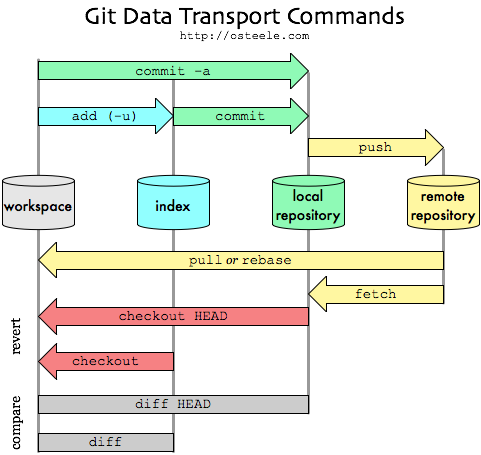
\includegraphics[keepaspectratio,width=0.5\paperwidth]{Pictures/git_dataflow.png}
    \end{center}
    \caption{Git数据流}
\end{figure}

\subsection{配置}
配置彩色界面
\begin{verbatim}
git config --global color.ui true
\end{verbatim}

\subsection{基本用法}
创建版本库

\begin{verbatim}
git init
\end{verbatim}

添加文件并提交

\begin{verbatim}
git add -A
git commit -m ``initialized''
\end{verbatim}


修改文件并提交
\begin{verbatim}
git commit -a
\end{verbatim}

撤销工作区修改
\begin{verbatim}
git checkout -- . 撤销修改,用暂存区覆盖工作区
git checkout .  同上
\end{verbatim}

查看历史
\begin{verbatim}
git log <refs>本分支提交历史
git log -3 只显示最近3次提交
git log --stat 显示修改统计
git reflog [show] <refs> 引用历史
\end{verbatim}

查看文件状态
\begin{verbatim}
git checkout [HEAD] 显示工作区、暂存区、HEAD之间的差异
git status
git ls-files [-c] 查看暂存区文件
git ls-files -m 查看被修改的文件
git ls-files -d 查看被删除的文件
git ls-files -o 查看其他文件,即未被追踪的文件
git write tree; git ls-tree <treeish> 查看tree包含的blob
\end{verbatim}

检出历史文件
\begin{verbatim}
git checkout <commit> [--] filename
省略commit,则表示暂存区。
\end{verbatim}

整体回归历史
\begin{verbatim}
git reset --hard <id> 
提交日志也会一起回归历史
git checkout <id> 
会进入分离头指针状态,此后的提交日志不容易查看
git checkout -b <new_branch> <id>
新建分支,回归历史
\end{verbatim}
总之,checkout命令修改HEAD指向,reset修改分支指向

修改刚才的提交的提交说明
\begin{verbatim}
git commit --amend
\end{verbatim}

修改某个历史提交的提交说明
\begin{verbatim}
git rebase -i <some history>
\end{verbatim}

将从v1开始的历次提交逐一导出为补丁
\begin{verbatim}
git format-patch v1..HEAD
\end{verbatim}

不慎提交了不想提交的文件,如winxp.img
\begin{verbatim}
git rm --cached winxp.img
git commit --amend
\end{verbatim}
git rm将文件从工作区和index同时删除。--cache指定不从工作区删除。

比较差异:
比较工作区和暂存区:git diff
比较工作区与HEAD:git diff HEAD
比较工作区与里程碑A:git diff A
比较暂存区与里程碑A:git diff --cached A
比较暂存区与HEAD:git diff --cached
比较里程碑A和B git diff B A

\subsection{显示id}
\begin{verbatim}
git rev-parse master
\end{verbatim}

创建里程碑``v1''
\begin{verbatim}
git tag v1
\end{verbatim}




\section{Indent代码排版工具}

欲实现Cavium风格的代码,有
\begin{verbatim}
indent *.c -bli0 -i4 -npsl -cli4 -npcs
\end{verbatim}

其中,bli表示brace indentation, i选项表示indentation, npsl(dont-break-procedure-type)表示函数返回类型需与函数名称在同一行;cli表示case-label-indentation, 表示case语言缩进的距离。npcs表示no-sapce-after-function-call-names,函数调用时函数名称后无空格。

关于if等语句之后的\verb+{+括号是否在换行,有两种方式:br(braces-on-if-line)和bl(braces-after-if-line)。对于br选项,一般同时指定ce选项(cuddle-else)或nce选项,前者让\verb+}+和else在同一行。对于bl选项,一般同时指定bli选项,表示\verb+{+缩进距离,如不指定,GNU indent默认使用GNU风格,即缩进2个空格。类似于if语句,函数定义和struct定义也存在大括号是否在同一行的问题。对于函数,可以指定brf或blf(默认);对于struct,可以指定brs和blf。
\section{Nerd注释插件用法}
\begin{verbatim}
简单介绍下NERD Commenter的常用键绑定,以C/C++文件为例,详析的使用方法,请:h NERDCommenter。在Normal或者Visual 模式下:

,ca,在可选的注释方式之间切换,比如C/C++ 的块注释/* */和行注释//

,cc,注释当前行

,c,切换注释/非注释状态

,cs,以”性感”的方式注释

,cA,在当前行尾添加注释符,并进入Insert模式

,cu,取消注释

Normal模式下,几乎所有命令前面都可以指定行数

Visual模式下执行命令,会对选中的特定区块进行注释/反注释

注:各命令前缀是可以自己设置的,通常是逗号’,'或者’\’.
\end{verbatim}
\section{Python IDE选用}

\subsection{Vim搭建Python IDE}
Vim插件pythonComplete可用于Python代码自动补全。对于VIM 7.3以上版本,这个插件是自带的。需要在.vimrc上添加如下配置:
\begin{verbatim}
filetype plugin on  
autocmd FileType python set omnifunc=pythoncomplete#Complete  
\end{verbatim}

\subsection{ctags配置}
ctags也支持Python语言:
\begin{verbatim}
ctags -R
ctags -R --language-force=Python --Python-kinds=cfmvi --extra=+q
\end{verbatim}

\subsection{Eric}
Eric是基于Qt的IDE,依赖于包python-qscintilla2。

\subsection{IDLE}
IDLE常常是python安装是自带的开发工具。

\section{Subversion版本修订控制}
checkout(co)操作

\begin{verbatim}
svn checkout http://svn.example.com:9834/repos
svn checkout file:///var/svn/repos
svn co https://svn.sinaapp.com/myhello(新浪云平台) 
\end{verbatim}

添加文件:
\begin{verbatim}
svn add DIRNAME/
\end{verbatim}

提交文件:
\begin{verbatim}
svn ci -m ``MESSAGE''
\end{verbatim}






\section{Vim之taglist插件}
用法:
\begin{verbatim}
:TlistToggle 打开或关闭列表
<CR> 跳转至列表所指对象
<Space> 显示原型
u 更新列表
s 更新排序方式(按出场顺序或名称)
x 伸缩列表宽度
\end{verbatim}

常见设置(.vimrc)
\begin{verbatim}
let Tlist_Show_One_File = 1            "不同时显示多个文件的tag,只显示当前文件的
let Tlist_Exit_OnlyWindow = 1          "如果taglist窗口是最后一个窗口,则退出vim
let Tlist_Use_Right_Window = 1         "在右侧窗口中显示taglist窗口
let Tlist_GainFocus_On_ToggleOpen = 1
map <silent> <leader>tl :TlistToggle<cr>
\end{verbatim}


\section{UML正反向工程}
umbrello:不能包含c语言标准库的文件,如
\verb+#include <time.h>+
否则程序会崩溃
\section{Vim文本编辑}


\subsection{快速键入}
本节C表示Ctrl键。
在insert模式下:\\
C-W 删除当前单词(同Bash) \\
C-U 删除当前句子(同Bash)\\
C-P,C-N  自动补全,补全内容分别从前方或后方搜索\\
C-A 键入上次在INSERT模式下键入的内容,并进入INSERT模式\\
C-Y 键入上次在INSERT模式下键入的内容\\
C-X C-F 自动补全,文件名\\
C-X C-L 自动补全,整行\\
C-X C-D  自动补全,宏定义\\

在Normal模式下,CTRL A 和CTRL X分别将光标下的数字加1或减1

\subsection{快速配对区域操作}
快速处理\verb+''、""、()、[]、{}、<> +等配对标点符号中的文本内容,包括更改、删除、复制等。
\begin{verbatim}
ci(  快速修改()内的内容,即删除后进入insert模式
di(  快速删除()内的内容
yi(  快速复制()内的内容
\end{verbatim}
将上述i替换为a,()本身也会被选取。


\subsection{跨文档复制粘贴}
一般地,复制到指定寄存器的方法为:

普通模式下\verb|"+寄存器名+y|。

插入某寄存器内容的方法为:

普通模式下\verb|"+寄存器名+p|或编辑模式下\verb|Ctrl+R+寄存器名|。

有两个特殊的寄存器: 选择寄存器(寄存器``)为可视模式下选择的内容,剪贴板(寄存器+)为用图形界面选择的内容。


\subsection{跨文件字符替换}
每个文件在vim被称为缓冲区。

方法一:命令录制。
\begin{verbatim}
qq,:wnext,q.
\end{verbatim}

方法二:bufdo, argdo, windo等。
\begin{verbatim}
:wa
:bufdo %s/foo/bar/ge |update
\end{verbatim}

\subsection{文档统计}
显示当前文件名称与行数
\begin{verbatim}
:f 或 Ctrl+G
\end{verbatim}
显示某单词word出现的次数
\begin{verbatim}
%s/word//gn
\end{verbatim}
中文字数统计(近似方法)
\begin{verbatim}
%s/\S//gn
缺点是将非中文字符也算做一个字,如英文单词、标点等。
:%s/[^[:print:][:cntrl:]]//gn
缺点是中文标点也算作了汉字
:%s/[\u4e00-\u9fa5]//gn
使用unicode匹配,不成功,可能是因为utf8编码的文件不支持unicode匹配
\end{verbatim}


注意wc -m命令也可以统计字符数,但是把空白字符也算作内了。

\subsection{基于空格的列操作}
\verb+\S,\s+分别表示非空格和空格,后带\verb%\+%表示至少为一。再结合括号和数字引用,可以基于空格进行各种列操作。

例1:在非空行前后添加内容:
\verb#:%s/^\s*\(\S\+.*\)$/haha;\1wawa;#

例2:只保留第一列,其余删除:
\verb%5,12s/\(\S\+\)\s\+.*/\1/g%

\subsection{折行的开与关}
zR 打开所有折行;zr打开下一级折行;zM关闭所有折行;zm 关闭上一级折行
zo 打开折行;zc 重新关闭折行
zf 创建折行;zfap zf命令作用于ap(一个段落)

\subsection{屏幕错乱}
Ctrl+L即可。

\subsection{键入特殊字符}
外国人姓名之间的点号:fcitx激活时键入[即可。
\begin{verbatim}
:digraphs 查看VIM支持的特殊字符
\end{verbatim}
Insert模式使用CTRL-K {key1 key2}键入特殊字符。
如输入拼音a的四个声调,分别为\verb+a-(或a~),a‘,a<,a`(或a!)+。希腊字符\[\alpha,\beta\]分别为\verb+a*, b*+。

\subsection{键入Unicode字符}
Insert模式使用CTRL-V {digits}来插入一个由{digits}指定其ASCII码的字符. 

用这种方法你可以插入0到255的所有字符.如果你键入的数字少于两个, 那么Vim会在遇到一个非数字字符时终止这个命令. 要避免非得键入一个非数字字符才能让这个命令结束,你可以在数字前加上一个或两个0来凑足3个数.

\begin{verbatim}
CTRL-V 009.
\end{verbatim}

要用十六进制来表示你的ASCII, 在CTRL-V后面附加一个"x":
\begin{verbatim}
CTRL-V x7f
\end{verbatim}

接下来的两个方法还可以让你键入一个16bit或32bit的数字(比如,用来指定一个Unicode字符):
\begin{verbatim}
CTRL-V o123
CTRL-V u1234
CTRL-V U12345678
\end{verbatim}

\subsection{快速插入日期}
可以定义如下键盘映射,使得在Insert模式下,F8可以键入日期:
\begin{verbatim}
imap <F8> <Esc>:read !date +\%F<CR>i
使用了date系统命令,\是为了转义%号,在Bash中不需要
格式%F相当于%Y-%m-%d
\end{verbatim}

\subsection{大小写替换}
在替换命令中,一个字符前面加\verb+\u+会被转为大写,\verb+\l+会被转为小写。


\subsection{列选择模式}
Normal模式下CtrlV会进入列选择模式,可以用来对表格的列进行选择操作。


\subsection{缩写}
iab命令定义在Insert模式下的缩写,如

\begin{verbatim}
iab ssend SSEND_HAHA
\end{verbatim}
iunab取消缩写,iab列出缩写。

\subsection{C程序缩进}
设置缩进为4,并用空格代替TAB:
\begin{verbatim}
set softtabstop=4
set shiftwidth=4
set expandtab
\end{verbatim}
== 为当前行整理缩进
=a{ 为当前代码块整理缩进
=G 从当前行到文件结尾,整理缩进
gg=G 为整个文件整理缩进


\subsection{英文拼写检查}
\begin{verbatim}
:setlocal spell spelllang=en_us 
:set spell
:setlocal nospell
:set nospell
\end{verbatim}


\subsection{vim选项的值}
\begin{verbatim}
:se[t] 显示所有不等于默认值的选项
:set all 显示所有选项
:set option? 显示选项的值
:set option 对于Toggle类型的选项,将其值设置为on;其他类型的选项,显示其值
\end{verbatim}

\subsection{重新载入vimrc}
\begin{verbatim}
:source ~/.vimrc
:so ~/.vimrc
\end{verbatim}


\section{在Vim中编写tex文件}

\subsection{latexsuite安装与配置}
\begin{shellcmd}
	sudo apt-get install vim-latexsuite
	vim-addons install latex-suite
\end{shellcmd}
意欲在打开tex文件时自动开启latexsuite,需配置.vimrc
详细参见help:latex-suite
\begin{verbatim}
    " REQUIRED. This makes vim invoke Latex-Suite when you open a tex file.
    filetype plugin on
    
    " IMPORTANT: win32 users will need to have 'shellslash' set so that latex
    " can be called correctly.
    set shellslash
    
    " IMPORTANT: grep will sometimes skip displaying the file name if you
    " search in a singe file. This will confuse Latex-Suite. Set your grep
    " program to always generate a file-name.
    set grepprg=grep\ -nH\ $*
    
    " OPTIONAL: This enables automatic indentation as you type.
    filetype indent on
    
    " OPTIONAL: Starting with Vim 7, the filetype of empty .tex files defaults to
    " 'plaintex' instead of 'tex', which results in vim-latex not being loaded.
    " The following changes the default filetype back to 'tex':
    let g:tex_flavor='latex'

\end{verbatim}

\subsection{配置文件}
配置文件texrc的路径为:
~/.vim/ftplugin/latex-suite
\subsection{环境插入}
F5用于输入环境。

\subsection{分节}
文档上给出了快捷键:
\begin{verbatim}
SPA for part
SCH for chapter
SSE for section
SSS for subsection
SS2 for subsubsection
SPG for paragraph
SSP for subparagraph
\end{verbatim}


\subsection{借助sort命令多域排序}
如果以\&为分隔符(常见于latex表格),第二列升序,第一列降序排序,则有:
\verb+sort -k 2n -k 1r -t'&' FILENAME+

\subsection{表格标记添加}
如果表格是从word或网页上拷贝的,则需要添加\&和换行符号。在vim中依次执行一下命令:
\begin{verbatim}
:22,40s/\s\+$//  #去除行尾空格
:22,40s/\(\s\+\)/\&\1/g #空格前添加&
:22,40s/$/\\\\/g #行尾添加\\符号
\end{verbatim}



\section{Vim跳转}

\subsection{同时打开两个文件}
\begin{verbatim}
vim -o a.txt b.txt 竖屏
vim -O a.txt b.txt 横屏
vim -p a.txt b.txt 多标签页
:new 新增空白窗口
Ctrl-w = 平分宽高,注意键入=时,ctrl和w必须松开
Ctrl-w +/> 增减高/宽
Ctrl-w -/< 减小高/宽
Ctrl-w 20< 宽度减小20个单位
20Ctrl-w < 宽度减小20个单位
:vertical res[ize] +8 宽度增减8
\end{verbatim}

\subsection{命令行窗口}
Normal模式下键入\verb+q:+。

\subsection{shell跳转}
\begin{verbatim}
:sh 暂时返回shell;exit会返回vim
ctrl+Z 将vi转入后台,用fg恢复vi
\end{verbatim}

\subsection{路径跳转}
\begin{verbatim}
:E[xplore] 裂屏显示文件目录
:Sex 同Explore, 但是是上下裂屏
\end{verbatim}

\subsection{文件跳转}
\begin{verbatim}
:find filename用于文件跳转。
:[vert] sfind filename裂屏跳转。
:tabfind filename 新建标签页并跳转
gf(goto file)跳转到光标下的文件。
\end{verbatim}

有时需要添加path信息,如
\begin{verbatim}
:set path+=<path to the file>
:set path 显示path的当前值
:checkpath 显示所有无法找到的#include文件
:checkpath! 显示所有#include文件
\end{verbatim}
当前目录下的文件不需要添加path信息。

我们还可以在这个命令中使用通配符来进行匹配,如:
\begin{verbatim}
:set path=/usr/include,/usr/include/*
\end{verbatim}
这样,\verb+:find stdio.h+就可以查看一些库文件。

**匹配整个目录树,如:
\begin{verbatim}
:set path=/usr/include/**
:set path=/home/oualline/progs/**/include
\end{verbatim}
空字符串指当前目录,.指我们正在编辑的文件所在的目录,例如下面的命令是告诉Vim查找的目录包括/usr/include及其所的子目录,我们正编辑的文件所在的目录(.)以及当前目录(空串):
\begin{verbatim}
:set path=/usr/include/**,.,,
\end{verbatim}

\subsection{语句跳转}
\begin{verbatim}
[/]{ 查找上/下一个层次高于当前位置的{,用于语句块跳转
[/]# 查找上/下一个层次高于当前位置的#,用于在#ifdef-#endif结构中跳转
[/]( 查找上/下一个层次高于当前位置的(,用于在条件表达式中跳转
[/]/ 查找上/下一个层次高于当前位置的/,用于在注释中跳转
[/][ 查找上/下一个层次为1的{,用于全局函数跳转
[/]m 查找上/下一个层次为1或2的{,在面向对象语言中method对应层次为2的{
{/} 转到上/下一个空行
*/# 转到当前光标所指的单词下/上一次出现的地方
\end{verbatim}
[I 会列出所有包含该标识符的行,其中第一行可能包含变量定义,搜索范围包括了include文件。

[I命令查找任何的标识符.要只查找宏使用[D。

[d显示[D的第一个结果,[i显示[I的第一个结果。

[+tab 跳转至函数声明或变量定义,估计就是[i所指示的结果。gD将搜索范围局限在了当前文件,gd将搜索范围局限在了当前函数。

\subsection{标签页操作}

\begin{verbatim}
vim -p file1 file2 ..
:tabnew file1
:tabe[dit] file2
:tabnew
:tab split
:tabs 显示所有标签页的信息
\end{verbatim}
使用标签页打开文件

\begin{verbatim}
:tabc :q 关闭当前标签页
:tabo 关闭所有标签页
gt 转入下一个标签页
gT 转入上一个标签页
3gt 转入第3个标签页
:tabn 转入下一个标签页
:tabp 转入上一个标签页
:tabfirst, :tablast 顾名思义
:tabdo cmd 对所有标签页执行命令
\end{verbatim}





\section{Nerd注释插件用法}
\begin{verbatim}
简单介绍下NERD Commenter的常用键绑定,以C/C++文件为例,详析的使用方法,请:h NERDCommenter。在Normal或者Visual 模式下:

,ca,在可选的注释方式之间切换,比如C/C++ 的块注释/* */和行注释//

,cc,注释当前行

,c,切换注释/非注释状态

,cs,以”性感”的方式注释

,cA,在当前行尾添加注释符,并进入Insert模式

,cu,取消注释

Normal模式下,几乎所有命令前面都可以指定行数

Visual模式下执行命令,会对选中的特定区块进行注释/反注释

注:各命令前缀是可以自己设置的,通常是逗号’,'或者’\’.
\end{verbatim}
\section{Python IDE选用}

\subsection{Vim搭建Python IDE}
Vim插件pythonComplete可用于Python代码自动补全。对于VIM 7.3以上版本,这个插件是自带的。需要在.vimrc上添加如下配置:
\begin{verbatim}
filetype plugin on  
autocmd FileType python set omnifunc=pythoncomplete#Complete  
\end{verbatim}

\subsection{ctags配置}
ctags也支持Python语言:
\begin{verbatim}
ctags -R
ctags -R --language-force=Python --Python-kinds=cfmvi --extra=+q
\end{verbatim}

\subsection{Eric}
Eric是基于Qt的IDE,依赖于包python-qscintilla2。

\subsection{IDLE}
IDLE常常是python安装是自带的开发工具。

\section{Vim之quickfix插件}
Vim标准插件,无需安装。

在代码窗口中执行:make命令后,按回车可以定位到第一个error或warning。

用法:
\begin{verbatim}
:cc                显示详细错误信息 ( :help :cc )
:cp                跳到上一个错误 ( :help :cp )
:cn                跳到下一个错误 ( :help :cn )
:cl                列出所有错误 ( :help :cl )
:cw                如果有错误列表,则打开quickfix窗口 ( :help :cw )
:col               到前一个旧的错误列表 ( :help :col )
:cnew              到后一个较新的错误列表 ( :help :cnew ) 
\end{verbatim}

常见设置(.vimrc)
\begin{verbatim}
"quickfix
nmap <F6> :cn<cr>
nmap <F7> :cp<cr>
\end{verbatim}


\section{Vim之taglist插件}
用法:
\begin{verbatim}
:TlistToggle 打开或关闭列表
<CR> 跳转至列表所指对象
<Space> 显示原型
u 更新列表
s 更新排序方式(按出场顺序或名称)
x 伸缩列表宽度
\end{verbatim}

常见设置(.vimrc)
\begin{verbatim}
let Tlist_Show_One_File = 1            "不同时显示多个文件的tag,只显示当前文件的
let Tlist_Exit_OnlyWindow = 1          "如果taglist窗口是最后一个窗口,则退出vim
let Tlist_Use_Right_Window = 1         "在右侧窗口中显示taglist窗口
let Tlist_GainFocus_On_ToggleOpen = 1
map <silent> <leader>tl :TlistToggle<cr>
\end{verbatim}



\chapter{其他桌面工具和技巧}
\section{实用计算、查询与搜索}

\subsection{算数}
Linux下一些CGI工具可以用作计算器,如Python,calc,bc等。

Python计算默认为整数计算,如需浮点数运算结果,可以在运算数后加.0;也可以在运行Python时使用命令行开关-Qnew

calc工具来自于apcalc软件包,可以实现任意精度的计算。calc默认就是浮点数计算,比较方便;而bc默认为整数计算。

bc其实是一种复杂的编程语言;如计算5/6, 设置精度为3位,则有:
\begin{verbatim}
	scale=3;5/6
\end{verbatim}

\subsection{进制转换}
可以用Python完成进制转换运算。

十进制转换为二进制、八进制、十六进制,可以分别使用函数bin,oct,hex。 
二进制,8进制,16进制转十进制容易,直接在互动界面上键入0xa3,0b101,0o33即可。

\subsection{ASCII码表}
可以查找man页:\verb+man ascii+
在Python下,十进制转ASCII可以用chr函数,反之使用ord。

\subsection{时间计算} 
Python的datetime包提供了日期与时间相关的操作。 参考\ref{sec:pythonTimeCalc}。

\subsection{日历查询}
cal工具能够打印某年或某月的日历,默认为本月。
\begin{verbatim}
cal #本月
cal 2012 #某年
cal -y 2012 #某年
cal -m 8 #今年某月
cal 8 2012 #某年某月
\end{verbatim}

calendar模块提供了查询平闰年和星期的功能,也能产生日历字符串。参考\ref{sec:pythonTimeCalc}。

\subsection{IP地址查询}
\begin{verbatim}
whois 202.38.95.110
\end{verbatim}

\subsection{Google汇率查询}
汇率查询,比如欲查询人民币和韩币汇率,Google:
\begin{verbatim}
cny in won
rmb in won
china in korea currency
\end{verbatim}

\subsection{Google单位换算}
\begin{verbatim}
mile to km
\end{verbatim}

\subsection{Google技巧}
\url{http://www.googleguide.com}.
布尔运算:与(空格默认为AND)、或(大写OR,|(vertical bar))、非(-)。\verb+()+可调整运算优先级。

域搜索:site, inurl, filetype。

精确搜索:双引号

前缀:allintitle,link

同时,Google提供了高级搜索的UI界面。

























\section{ImageMagick工具用法}
ImageMagic包含display,convert, identify, mogrify, montage, compare等工具。
\label{sec:imagemagick}

display用来看图片,如观看当前路径下所有图片,有
\begin{verbatim}
display *
\end{verbatim}

identify用来显示图片信息。

convert用来转换图片:
\begin{verbatim}
convert input-file [options] output-file
\end{verbatim}

pdf和图片相互转换,有
\begin{verbatim}
convert *.png output.pdf
convert haha.pdf 1.png pdf文件转换为前缀为1的png文件
\end{verbatim}

旋转图片
\begin{verbatim}
convert -rotate 90 image.jpg image.png
convert -flip a.jpg b.jpg 上下翻转
convert -flop a.jpg b.jpg 左右翻转
\end{verbatim}

图像加框
\begin{verbatim}
convert -border 60*60 “#000000″ a.jpg b.jpg
60*60是表示边框的宽度,第一个是纵边框的宽度,第二个是横边框的宽度
#000000是RGB格式的边框色彩
\end{verbatim}



以下命令用于改变图片大小(宽×高):
\begin{verbatim}

1. 默认时,宽度和高度表示要最终需要转换图像的最大尺寸,同时Convert会控制图片的宽和高,保证图片按比例进行缩放。

如:convert -resize 600×600 src.jpg dst.jpg

转换后的dst.jpg的图片大小(宽度为600,而高度已经按比例调整为450).

2.如果需要转换成600×600,而图片无需保持原有比例,可以在宽高后面加上一个感叹号!.

如:convert -resize 600×600! src.jpg dst.jpg

3. 只指定高度,图片会转换成指定的高度值,而宽度会按原始图片比例进行转换。

如:convert -resize 400 src.jpg dst.jpg

转换后的dst.jpg的图片大小(宽度为400,而高度已经按比例调整为300),和例1有点类似。

4. 默认都是使用像素作为单位,也可以使用百分比来形象图片的缩放。

如:convert -resize 50%x100%! src.jpg dst.jpg 或者convert -resize 50%x100% src.jpg dst.jpg

此参数只会按你的比例计算后缩放,不保持原有比例。(结果尺寸为100×150)

5.使用 @ 来制定图片的像素个数。

如:convert -resize “10000@” src.jpg dst.jpg

此命令执行后,dst.jpg图片大小为(115×86),图片保持原有比例(115×86= 9080 < 10000)。

6.当原始文件大于指定的宽高时,才进行图片放大缩小,可使用>命令后缀。

如:convert -resize “100×50>” src.jpg dst.jpg

此命令执行后,dst.jpg图片大小为(67×50),图片保持原有比例。

如:convert -resize “100×50>!” src.jpg dst.jpg

此命令执行后,dst.jpg图片大小为(100×50),图片不保持原有比例。

7.当原始文件小于指定的宽高时,才进行图片放大转换,可使用<命令后缀。

如:convert -resize “100×500<” src.jpg dst.jpg 或者convert -resize “100×100<!” src.jpg dst.jpg

此命令执行后,dst.jpg和src.jpg大小相同,因为原始图片宽比100大。

如:convert -resize “600×600<” src.jpg dst.jpg

此命令执行后,dst.jpg图片大小为(600×450),图片保持原有比例。

如:convert -resize “600×600<!” src.jpg dst.jpg

此命令执行后,dst.jpg图片大小为(600×600),图片不保持原有比例。

8.使用^命令后缀可以使用宽高中较小的那个值作为尺寸

如:convert -resize “300×300^” src.jpg dst.jpg

此命令执行后,dst.jpg图片大小为(400×300),图片保持原有比例,(300:300 < 200:150,选择高作为最小尺寸)。

如:convert -resize “300×200^” src.jpg dst.jpg

此命令执行后,dst.jpg图片大小为(300×225),图片保持原有比例,(300:200 > 200:150,选择宽作为最小尺寸)。


\end{verbatim}
\section{音视频播放与编辑}

\subsection{视频播放控制}
\subsubsection{mplayer}
文件打开命令:mplayer [-af scaletempo [-speed 0.01~100]] filename

其中,-af设置音频过滤器,scaletempo实现变速不变调(pitch)功能。详情见其help输出和man页。

快捷键(man页:INTERACTIVE CONTROL):
速度调节: 	[和],以10\%为幅度。
进度调节:	左右方向键以10s为精度,上下方向键以分钟为精度,翻页键以10min为精度。

\begin{verbatim}

 p or SPACE       pause movie (press any key to continue)
 q or ESC         stop playing and quit program
 + or -           adjust audio delay by +/- 0.1 second
 o                cycle OSD mode:  none / seekbar / seekbar + timer
 * or /           increase or decrease PCM volume
 x or z           adjust subtitle delay by +/- 0.1 second
 r or t           adjust subtitle position up/down, also see -vf expand

backspace          Reset playback speed to normal.
 f                 Toggle fullscreen (also see -fs).
 T                 Toggle stay-on-top (also see -ontop).

v                Toggle subtitle visibility.
j and J          Cycle through the available subtitles.
\end{verbatim}

\subsubsection{VLC}
详情见其help输出和man页。VLC默认为变速不变调。

速度调节:[和],同mplayer一样的快捷键,只是调节幅度为0.1倍原速。

进度调节:shift/alt/ctrl+左右方向键。shift的精度为5s,alt为10s,ctrl为1min。


\subsection{音视频文件编辑}
Linux下有OpenShot Video Editor。曾用它来裁剪视频文件。

跨平台开源软件audacity,操作方式类似于Adobe Audition(CoolEditPro,不支持Linux),可以看见音频波形。支持批量导入音频文件。

\section{网络通信工具}

\subsection{邮件提醒}

\begin{description}
    \item[Pidgin插件]安装pidgin-guifications插件,并设置Pidgin接收MSN邮件。
    \item[checkgmail]checkgmail可以检查Gmail邮箱。将所关注的邮箱设置成自动转发到gmail,设置gmail的动作为打开邮件客户端如evolution。
    \item[其他方案]mail-notification;gnubiff。
\end{description}

\subsection{即时通信}

常见的聊天工具如QQ,MSN和飞信都有网页版,可以用浏览器制作Web App。除此之外,还有一些第三方客户端。

飞信: Web飞信,3G飞信,openfetion,cliofetion,pidgin-openfetion。

QQ:Web Q+, libqq-pidgin(ppa:lainme/libqq,基于QQ国际版,已经失效),Wine-qq。基于Web QQ协议,分别有人使用Python,GTK,Qt,Java、Pidgin开发了QQ客户端,包括:python-webqq(ppa:linux-deepin-team/linux-deepin), gtkqq(ppa:bill-zt/gtkqq),QtQQ, iQQ,pidgin-lwqq(ppa:lainme/pidgin-lwqq)。

MSN:Web Windows Live,pidgin,aMSN,kmess, kopete, emesene,empathy等。

\subsection{聊天消息提醒}
Web Q+:桌面通知功能,可以实现跨工作区提醒,直接显示聊天内容于桌面。标题栏提醒功能,不能跨工作区提醒,不暴露消息内容。消息走马灯功能,尚不知如何使用。

Pidgin:libnotify插件,会弹出消息,不够隐私;guification(软件包pidgin-guifications)插件,和notify(中文:消息提示)插件,可以做到跨工作区提醒,不直接显示消息。后来发现notify插件没什么作用(Linux Deepin 12.06)。好友千里眼,添加对单独好友的新消息监视,一次性使用,也可以勾选“重复”,每条消息都会提示一次。最好的办法是右键面板图标,勾选“有新消息时闪烁”。

其他聊天工具具体情况有待补充。

\subsection{Chromium浏览器}
软件包叫做chromium-browser,默认不自带flash插件。需要安装flashplugin-installer。然后执行:
\begin{shellcmd}
    sudo cp /usr/lib/flashplugin-installer/\
    libflashplayer.so \ 
    /usr/lib/chromium-browser/
\end{shellcmd}

\subsection{远程登录}
ssh远程登录:sshpass,lcrt。lcrt是为数不多的能保存密码的ssh登录工具。

\section{PDF阅读、编辑和转换}

\subsection{PDF阅读与批注}
acroread软件包包含了Adobe Reader, 兼容性好,可以调节背景色。但功能相对于Acrobat十分受限, 没有批注、书签等功能,运行效率也低下。

okular可以实现pdf的批注(F6或tools->review)和背景色改变。其缺点是,如果在gnome环境下安装需要下载几十MB的包。

mendeley可以实现批注,但批注只是内部识别。不能调节背景色。

xournal添加文字注释,下划线,通过export功能保存修改结果;但是Xournal对于篇幅较长的PDF文档太耗尽内存,因为它会将PDF文档中所有的页面都转化为图像数据置于内存之中并且不再释放。我们可以首先对文档进行分割。据说只要别大范围拖动滚动条,内存占用便不大。

evince,Foxit4Linux,永中阅读器既不能标记,又不能改变背景色。

综上,对于pdf阅读,较好的有okular,wine上的foxit,cajviewer。

pdfgrep(CLI)可以从pdf中查找正则表达式,用法类似于grep。diffpdf可以比较两个pdf文件的不同。

\subsection{PDF书签编辑}
pdfmod是目前发现的唯一一个制作书签的开源工具,但编辑不便,无法调整书签的显示顺序。Windows下的Foxit Reader可以制作pdf书签,linux版本的则不可。evince制作的书签似乎只是内部识别。因此,在Linux下最好wine一个Windows版的Foxit Reader。

\subsection{PDF页面级编辑}

pdfshuffler可以合并、分裂、排序页面,在precise pangolion尝试出错,显示没有EOF标记。

pdftk为CLI工具,功能包括合并,分裂,删页,反序,旋转,加解密,其中合并pdf的方式包括连接和互插。pdfchain是pdftk的一个GUI前端。

pdfmod可以用于删页、插入其他文件、导出页面、修改各页相对顺序(通过鼠标拖动,有时比pdftk方便)、编辑索引(书签),修改文件属性。

\subsection{PDF元素级编辑}
pdfedit添加文字注释(英文),划线,删除文档元素,删加页面;感觉不太稳定,运行十分缓慢,经常在打开文件时内核转储。

可以使用inscape或gimp提取PDF中的一页,进行复杂的修改,然后使用pdf删除合并工具恢复成完整的PDF文件。

openoffice.org-pdfimport包让LibreOffice能够直接导入PDF文件,进行文字修改,再保存为odg图形文件,或者选择导出为pdf。但导入PDF时文件内的图片常常会丢失,排版可能会被破坏。所以LibreOffice目前还不能算作PDF阅读器或者编辑器。

flpsed可以添加英文文字,但可能会损坏PDF,使其不能被其他阅读器打开。

pdfstudio功能强大,但系付费软件。

\subsection{PDF元数据}
pdfmod可以修改文件元数据,如作者、标题等。pdfinfo命令行工具可以显示元数据。
pdffonts显示文件字体信息。

\subsection{PDF格式转换}
ImageMagick可以实现pdf和图片的相互转换, 使用convert命令。
\begin{verbatim}
 convert [input-options] input-file [output-options] output-file
\end{verbatim}

\begin{verbatim}
convert -density 700 -quality 100 draft.pdf draft.jpg
\end{verbatim}
详细内容参\ref{sec:imagemagick}。

cups-pdf用于将其他格式的文件如图片打印为pdf。cups-pdf打印保存位置由/etc/cups/cups-pdf.conf文件配置,一般为~/PDF,或者/var/spool/cups-pdf。

pdftotext实现pdf到文本的转换,效果一般不理想。

gpdftext是一款编辑器,可以直接导入pdf文件进行文字编辑,再保存成文本或pdf格式,但是会丢失所有除文字内容之外的信息,包括格式、排版、分页信息。

pdftohtml实现pdf到html的转换,效果往往不理想。可能需要指定编码格式,如
\verb+pdftohtml -enc GBK haha.pdf +

pdfimages提取pdf中的图片,默认保存为ppm格式。
\verb+pdfimages -j haha.pdf+。
j选项指定保存为jpg格式。

pdf2ps和ps2pdf实现pdf和ps之间的转换,基于ghostscript机制。当前ps2pdf默认使用ps2pdf14,即pdf为1.4版本。可以直接使用ps2pdf15.pdftops也能实现pdf到ps之间的转换。

pdf2djvu,pdf2dsc,pdftoppm, pdf2svg分别实现pdf到djvu,dsc,ppm, svg的转换。SVG可缩放矢量图形(Scalable Vector Graphics)是基于  svg logo可扩展标记语言(XML),用于描述二维矢量图形的一种图形格式。

chm2pdf可以将chm转换为pdf。



\section{访问铁道部网站}
网购火车票的网址是http://www.12306.cn.sixxs.org/mormhweb/kyfw/,这个是http的普通网页,里面有个iframe,也就是嵌套了另一个网页,地址是https://dynamic.12306.cn/otsweb/,这里就是https的了。因为dynamic.12306.cn使用的是SRCA颁发的证书,这个证书在我们的计算机中是默认不被信任的,也就是不安全的。


火狐下解决办法:
\begin{verbatim}
1.在authorities导入铁道部根证书,编辑->首选项->高级->加密->查看证书->导入
2.打开https://dynamic.12306.cn/otsweb/,然后有提示将该网站添加例外即可
\end{verbatim}
\section{wget下载网站}
例如:
\begin{shellcmd}
wget -r -p -np -k http://www.21cn.com
wget --ftp-user=... --ftp-password=PASS  -r -p -np -k ftp://www.21cn.com
wget -r -p -np -k http://192.168.1.199/svn/OCTEON-SDK/branches/2012-03-27/OCTEON-SDK/docs/ --user=limz --password=123456
\end{shellcmd}


\section{Windows的U盘启动与U盘安装}
在百度百科上对相关主题有详细解释。

常用的工具有:老毛桃WinPE,一键U盘装系统,微软发布的Windows7 USB/DVD Download tool,U速启。

UltraISO也可以制作启动盘。 

HopedotVOS提供一个可以在U盘上运行的虚拟操作系统。


\part{计算机程序设计}
\chapter{编程方法杂谈}
\section{编程语言基础知识}

Programming language generations
 1GL为机器语言,2GL为汇编,3GL包括C, C++, C\#, Java, BASIC and Pascal。(4GL),基本上是传统软件工程界为了“范式开发” (prototyping) 而设计出来的语言,同时具有程序性与非程序性(就是宣告性)的特性,用来快速开发连接数据库的编程语言。如今天的 PowerBuilder 、 SQLWindows 等等。A fifth-generation programming language (abbreviated 5GL) is a programming language based on solving problems using constraints given to the program, rather than using an algorithm written by a programmer. "Generational" classification of high level languages (3rd generation and later) was never fully precise and was later perhaps abandoned, with more precise classifications gaining common usage, such as object-oriented, declarative and functional.

A domain-specific language (DSL) is a type of programming language or specification language in software development and domain engineering dedicated to a particular problem domain, a particular problem representation technique, and/or a particular solution technique.The opposite is:a general-purpose programming language, such as C, Java or Python,or a general-purpose modeling language such as the Unified Modeling Language (UML).


Query languages are computer languages used to make queries into databases and information systems.Broadly, query languages can be classified according to whether they are database query languages or information retrieval query languages. The difference is that a database query language attempts to give factual answers to factual questions, while an information retrieval query language attempts to find documents containing information that is relevant to an area of inquiry.

In computer programming, create, read, update and delete (CRUD) are the four basic functions of persistent storage.

A data manipulation language (DML) is a family of syntax elements similar to a computer programming language used for inserting, deleting and updating data in a database. Performing read-only queries of data is sometimes also considered a component of DML.Data manipulation languages are divided into two types, procedural programming and declarative programming.Procedural programming can sometimes be used as a synonym for imperative programming (命令式,specifying the steps the program must take to reach the desired state).Procedural programming languages include C, C++, Fortran, Pascal, and BASIC.


Each SQL DML statement is a declarative command. The individual SQL statements are declarative, as opposed to imperative, in that they describe the program's purpose, rather than describing the procedure for accomplishing it.

参数化查询(Parameterized Query 或 Parameterized Statement)是指在设计与数据库链接并访问数据时,在需要填入数值或数据的地方,使用参数 (Parameter) 来给值,这个方法目前已被视为最有效可预防SQL注入攻击 (SQL Injection) 的攻击手法的防御方式。
有部份的开发人员可能会认为使用参数化查询,会让程序更不好维护,或者在实现部份功能上会非常不便[来源请求],然而,使用参数化查询造成的额外开发成本,通常都远低于因为SQL注入攻击漏洞被发现而遭受攻击,所造成的重大损失。
除了安全因素,相比起拼接字符串的 SQL 语句,参数化的查询往往有性能优势。因为参数化的查询能让不同的数据通过参数到达数据库,从而公用同一条 SQL 语句。大多数数据库会缓存解释 SQL 语句产生的字节码而省下重复解析的开销。如果采取拼接字符串的 SQL 语句,则会由于操作数据是 SQL 语句的一部分而非参数的一部分,而反复大量解释 SQL 语句产生不必要的开销。

\section{程序员的十层楼}
\begin{verbatim}
自西方文艺复兴以来,中国在自然科学方面落后西方很多,软件领域也不例外。当然现在中国的许多程序员们对此可能有许多不同的意见,有些人认为中国的程序员水平远落后于西方,有些则认为中国的程序员个人能力并不比西方的程序员差,只是整个软件产业落后而已。

    那么,到底中国的程序员水平比西方程序员水平差,还是中国有许多优秀的程序员达到或超过了西方程序员同等水平呢?要解决这个问题,必须先知道程序员有多少种技术层级,每个层级需要什么样的技术水平,然后再比较中国和西方在各个技术层级的人数,就可以知道到底有没有差距,差距有多大。

    当然,对于如何划分程序员的技术层级,不同公司或不同人会有不同的划分标准,下面的划分仅代表个人的观点,如有不当之处,还请砸板砖予以纠正。

    第1层  菜鸟

    第1层楼属于地板层,迈进这层楼的门槛是很低的。基本上懂计算机的基本操作,了解计算机专业的一些基础知识,掌握一门基本的编程语言如C/C++,或者Java,或者JavaScript,...,均可入门迈进这层。

    在这层上,中国有着绝对的优势,除了从计算机专业毕业的众多人数外,还有大量的通信、自动化、数学等相关专业的人士进入这一行,此外还有众多的其他专业转行的人士,人数绝对比西方多出甚多。并且还有一个优势就是我们这层人员的平均智商比西方肯定高。

    没有多少人愿意一辈子做菜鸟,因为做"菜鸟"的滋味实在是不咋的,整天被老大们吆喝着去装装机器,搭建一下测试环境,或者对照着别人写好的测试用例做一些黑盒测试,好一点的可以被安排去写一点测试代码。当然如果运气"好"的话,碰到了国内的一些作坊式的公司,也有机会去写一些正式的代码。

    所以,菜鸟们总是在努力学习,希望爬更高的一层楼去。

    第2层 大虾

    从第1层爬到第2层相对容易一些,以C/C++程序员为例,只要熟练掌握C/C++编程语言,掌握C标准库和常用的各种数据结构算法,掌握STL的基本实现和使用方法,掌握多线程编程基础知识,掌握一种开发环境,再对各种操作系统的API都去使用一下,搞网络编程的当然对socket编程要好好掌握一下,然后再学习一些面向对象的设计知识和设计模式等,学习一些测试、软件工程和质量控制的基本知识,大部分人经过2~3年的努力,都可以爬到第2层,晋升为"大虾"。

    中国的"大虾"数量和"菜鸟"数量估计不会少多少,所以这层上仍然远领先于西方。

    大虾们通常还是有些自知之明,知道自己只能实现一些简单的功能,做不了大的东西,有时候还会遇到一些疑难问题给卡住,所以他们对那些大牛级的人物通常是非常崇拜的,国外的如Robert C. Martin、Linus Torvalds,国内的如求伯君、王志东等通常是他们崇拜的对象。其中的有些人希望有一天也能达到这些大牛级人物的水平,所以他们继续往楼上爬去。

    第3层 牛人

    由于"大虾"们经常被一些疑难问题给卡住,所以有了"大虾"们只好继续学习,他们需要将原来所学的知识进一步熟练掌握,比如以熟练掌握C++编程语言为例,除了学一些基础性的C++书籍如《C++ Primer》,《Effective C++》,《Think in C++》,《Exception C++》等之外,更重要的是需要了解C++编译器的原理和实现机制,了解操作系统中的内部机制如内存管理、进程和线程的管理机制,了解处理器的基础知识和代码优化的方法,此外还需要更深入地学习更多的数据结构与算法,掌握更深入的测试和调试知识以及质量管理和控制方法,对各种设计方法有更好的理解等。

    学习上面说的这些知识不是一挥而就的,不看个三五十本书并掌握它是做不到的。以数据结构算法来说,至少要看个5~10本这方面的著作;以软件设计来说,光懂结构化设计、面向对象设计和一些设计模式是不够的,还要了解软件架构设计、交互设计、面向方面的设计、面向使用的设计、面向数据结构算法的设计、情感化设计等,否则是很难进到这个楼层的。

    当然除了上面说的知识外,大虾们还需要去学习各种经验和技巧。当然这点难不倒他们,现在出版的书籍众多,网络上的技术文章更是不胜数,然后再去各种专业论坛里泡一泡,把这些书籍和文章中的各种经验、技能、技巧掌握下来,再去学习一些知名的开源项目如Apache或Linux操作系统的源代码实现等。此时对付一般的疑难问题通常都不在话下,菜鸟和大虾们会觉得你很"牛",你也就爬到了第3层,晋升为"牛人"了。

    看了上面所讲的要求,可能有些大虾要晕过去了,成为牛人要学这么多东西啊!要求是不是太高了?其实要求一点也不高,这么点东西都掌握不了的话,怎么能让别人觉得你"牛"呢?

    需要提一下的是,进入多核时代后,从第2层爬到第3层增加了一道多核编程的门槛。当然要迈过这道门槛并不难,已经有很多前辈高人迈进了这道门槛,只要循着他们的足迹前进就可以了。想迈进这道门槛者不妨去学习一下TBB开源项目的源代码(链接:http://www.threadingbuildingblocks.org/),然后上Intel的博客(http://softwareblogs-zho.intel.com/)和多核论坛(http://forum.csdn.net/Intel/IntelMulti-core/)去看看相关文章,再买上几本相关的书籍学习一下。

    在国内, 一旦成为"牛人",通常可以到许多知名的公司里去,运气好者可以挂上一个架构师的头衔,甚至挂上一个"首席架构师"或者"首席xx学家"的头衔也不足为奇。有不少爬到这层的人就以为到了楼顶了,可以眼睛往天上看了,开始目空一切起来,以为自己什么都可以做了,什么都懂了,经常在网络上乱砸板砖是这个群体的最好写照。由此也看出,国内的牛人数量仍然众多,远多于西方的牛人数量,在这层上仍然是领先的。

    也有不少谦虚的"牛人",知道自己现在还不到半桶水阶段。他们深知爬楼的游戏就像猴子上树一样,往下看是笑脸,往上看是屁股。为了多看笑脸,少看屁股,他们并没有在此停步不前,而是继续寻找到更上一层的楼梯,以便继续往上爬。

    第4层 大牛

    从第3层爬到第4层可不像上面说过的那几层一样容易,要成为大牛的话,你必须要能做牛人们做不了的事情,解决牛人们解决不了问题。比如牛人们通常都不懂写操作系统,不会写编译器,不懂得TCP/IP协议的底层实现,如果你有能力将其中的任何一个实现得象模象样的话,那么你就从牛人升级为"大牛"了。

    当然,由于各个专业领域的差别,这里举操作系统、编译器、TCP/IP协议只是作为例子,并不代表成为"大牛"一定需要掌握这些知识,以时下热门的多核编程来说,如果你能比牛人们更深入地掌握其中的各种思想原理,能更加自如的运用,并有能力去实现一个象开源项目TBB库一样的东西,也可以成为"大牛",又或者你能写出一个类似Apache一样的服务器,或者写出一个数据库,都可以成为"大牛"。

    要成为"大牛"并不是一件简单的事情,需要付出比牛人们多得多的努力,一般来说,至少要看过200~400本左右的专业书籍并好好掌握它,除此之外,还得经常关注网络和期刊杂志上的各种最新信息。

    当"牛人"晋升为"大牛",让"牛人们"发现有比他们更牛的人时,对"牛人"们的心灵的震撼是可想而知的。由于牛人们的数量庞大,并且牛人对大虾和菜鸟阶层有言传身教的影响,所以大牛们通常能获得非常高的社会知名度,几乎可以用"引无数菜鸟、大虾、牛人竞折腰"来形容,看看前面提过的Linus Torvalds等大牛,应该知道此言不虚。

    虽然成为"大牛"的条件看起来似乎很高似的,但是这层楼并不是很难爬的一层,只要通过一定的努力,素质不是很差,还是有许多"牛人"可以爬到这一层的。由此可知,"大牛"这个楼层的人数其实并不像想像的那么少,例如比尔middot;盖茨之类的人好像也是属于这一层的。

    由于"大牛"这层的人数不少,所以也很难统计除到底是中国的"大牛"数量多还是西方的大牛数量多?我估计应该是个旗鼓相当的数量,或者中国的"大牛"们会更多一些。

    看到这里,可能会有很多人会以为我在这里说瞎话,Linus Torvalds写出了著名的Linux操作系统,我国并没有人写出过类似的东西啊,我国的"大牛"怎么能和西方的比呢? 不知大家注意到没有,Linus Torvalds只是写出了一个"象模象样"的操作系统雏形,Linux后来真正发展成闻名全球的开源操作系统期间,完全是因为许多支持开源的商业公司如IBM等,派出了许多比Linus Torvalds更高楼层的幕后英雄在里面把它开发出来的。

    可能有些菜鸟认为Linus Torvalds是程序员中的上帝,不妨说个小故事:

    Linus,Richard Stallman和Don Knuth(高德纳)一同参加一个会议。

    Linus 说:"上帝说我创造了世界上最优秀的操作系统。"

    Richard Stallman自然不甘示弱地说:"上帝说我创造了世界上最好用的编译器。"

    Don Knuth一脸疑惑的说:"等等,等等,我什么时候说过这些话?"

    由此可以看出,Linus Torvalds的技术水平并不像想像中那么高,只是"牛人"和"大虾"觉得"大牛"比他们更牛吧了。在我国,有一些当时还处于"大虾"层的人物,也能写出介绍如何写操作系统的书,并且书写得非常出色,而且写出了一个有那么一点点象模象样的操作系统来。我想中国的"大牛"们是不会比西方差的,之所以没有人写出类似的商业产品来,完全是社会环境的原因,并不是技术能力达不到的原因。

    "大牛"们之所以成为大牛,主要的原因是因为把"牛人"给盖了下去,并不是他们自己觉得如何牛。也许有很多菜鸟、大虾甚至牛人觉得"大牛"这层已经到顶了,但大多数"大牛"估计应该是有自知之明的,他们知道自己现在还没有爬到半山腰,也就勉强能算个半桶水的水平,其中有些爬到这层没有累趴下,仍然能量充沛,并且又有志者,还是会继续往更上一层楼爬的。

    看到这里,也许有些菜鸟、大虾、牛人想不明白了,还有比"大牛"们更高的楼层,那会是什么样的楼层?下面就来看看第5层楼的奥妙。

    第5层 专家

    当大牛们真正动手做一个操作系统或者类似的其他软件时,他们就会发现自己的基本功仍然有很多的不足。以内存管理为例,如果直接抄袭Linux或者其他开源操作系统的内存管理算法,会被人看不起的,如果自动动手实现一个内存管理算法,他会发现现在有关内存管理方法的算法数量众多,自己并没有全部学过和实践过,不知道到底该用那种内存管理算法。

    看到这里,可能有些人已经明白第5层楼的奥妙了,那就是需要做基础研究,当然在计算机里,最重要的就是"计算"二字,程序员要做基础研究,主要的内容就是研究非数值"计算"。

    非数值计算可是一个非常庞大的领域,不仅时下热门的"多核计算"与"云计算"属于非数值计算范畴,就是软件需求、设计、测试、调试、评估、质量控制、软件工程等本质上也属于非数值计算的范畴,甚至芯片硬件设计也同样牵涉到非数值计算。如果你还没有真正领悟"计算"二字的含义,那么你就没有机会进到这层楼来。

    可能有人仍然没有明白为什么比尔·盖茨被划在了大牛层,没有进到这层来。虽然比尔·盖茨大学未毕业,学历不够,但是家有藏书2万余册,进入软件这个行业比绝大部分人都早,撇开他的商业才能不谈,即使只看他的技术水平,也可以算得上是学富五车,顶上几个普通的计算机软件博士之和是没有问题的,比起Linus Torvalds之类的"大牛"们应该技高一筹才对,怎么还进不了这层楼呢?

    非常遗憾的是,从Windows操作系统的实现来看,其对计算的理解是很肤浅的,如果把Google对计算方面的理解比做大学生,比尔·盖茨只能算做一个初中生,所以比尔·盖茨永远只能做个大牛人,成不了"专家"。

    看到这里,也许国内的大牛们要高兴起来了,原来比尔·盖茨也只和我等在同一个层次,只要再升一层就可以超越比尔·盖茨了。不过爬到这层可没有从"牛人"升为"大牛"那么简单,人家比尔middot;盖茨都家有2万多册书,让你看个500~1000本以上的专业书籍并掌握好它应该要求不高吧。当然,这并不是主要的条件,更重要的是,需要到专业的学术站点去学习了,到ACM,IEEE,Elsevier,SpringerLink,SIAM等地方去下载论文应该成为你的定期功课,使用Google搜索引擎中的学术搜索更是应该成为你的日常必修课。此外,你还得经常关注是否有与你研究相关的开源项目冒出来,例如当听到有TBB这样针对多核的开源项目时,你应该第一时间到Google里输入"TBB"搜索一下,将其源代码下载下来好好研究一番,这样也许你的一只脚已经快迈进了这层楼的门槛。

    当你象我上面说的那样去做了以后,随着时间的推移,总会有某天,你发现,在很多小的领域里,你已经学不到什么新东西了,所有最新出来的研究成果你几乎都知道。此时你会发现你比在做"牛人"和"大牛"时的水平不知高出了多少,但是你一点也"牛"不起来,因为你学的知识和思想都是别人提出来的,你自己并没有多少自己的知识和思想分享给别人,所以你还得继续往楼上爬才行。

    我不知道国内的"专家"到底有多少,不过有一点可以肯定的是,如果把那些专门蒙大家的"砖家"也算上的话,我们的砖家比西方的要多得多。

    第6层 学者

    当"专家"们想继续往上一层楼爬时,他们几乎一眼就可以看到楼梯的入口,不过令他们吃惊的是,楼梯入口处竖了一道高高的门槛,上面写着"创新"二字。不幸的是,大多数人在爬到第5层楼时已经体能消耗过度,无力翻过这道门槛。

    有少数体能充足者,可以轻易翻越这道门槛,但是并不意味着体力消耗过度者就无法翻越,因为你只是暂时还没有掌握恢复体能的方法而已,当掌握了恢复体能的方法,将体能恢复后,你就可以轻易地翻越这道门槛了。

    怎么才能将体能恢复呢?我们的老祖宗"孔子"早就教导过我们"温故而知新",在英文里,研究的单词是"research",其前缀"re"和"search"分别是什么意思不用我解释吧。或许有些人觉得"温故而知新"和"research"有些抽象,不好理解,我再给打个简单的比方,比如你在爬一座高山,爬了半天,中途体力不支,怎么恢复体力呢?自然是休息一下,重新进食一些食物,体力很快就可以得到恢复。

    由此可知,对体能消耗过度者,休息+重新进食通常是恢复体能的最佳选择。可惜的是,国内的老板们并不懂得这点,他们的公司里不仅连正常国家规定的休息时间都不给足,有些公司甚至有员工"过劳死"出现。所以国内能翻越"创新"这道门槛的人是"少之又少",和西方比起来估计是数量级的差别。

    再说说重新进食的问题,这个重新进食是有讲究的,需要进食一些基础性易消化的简单食物,不能进食山珍海味级的复杂食物,否则很难快速吸收。以查找为例,并不是去天天盯着那些复杂的查找结构和算法进行研究,你需要做的是将二分查找、哈希查找、普通二叉树查找等基础性的知识好好地复习几遍。

    以哈希查找为例,首先你需要去将各种冲突解决方法如链式结构、二次哈希等编写一遍,再试试不同种类的哈希函数,然后还需要试试在硬盘中如何实现哈希查找,并考虑数据从硬盘读到内存后,如何组织硬盘中的数据才能快速地在内存中构建出哈希表来,...,这样你可能需要将一个哈希表写上十几个不同的版本,并比较各个版本的性能、功能方面的区别和适用范围。

    总之,对任何一种简单的东西,你需要考虑各种各样的需求,以需求来驱动研究。最后你将各种最基础性的查找结构和算法都了然于胸后,或许某天你再看其他更复杂的查找算法,或者你在散步时,脑袋里灵光一现,突然间就发现了更好的方法,也就从专家晋升为"学者"了。

    学者所做的事情,通常都是在前人的基础上,进行一些小的优化和改进,例如别人发明了链式基数排序的方法,你第1个发现使用一定的方法,可以用数组替代链表进行基数排序,性能还能得到进一步提高。

    由于学者需要的只是一些小的优化改进,因此中国还是有一定数量的学者。不过和国外的数量比起来,估计少了一个数量级而已。

    也许有人会觉得现在中国许多公司申请专利的数量达到甚至超过西方发达国家了,我们的学者数量应该不会比他们少多少。因此,有必要把专利和这里说的创新的区别解释一下。

    所谓专利者,只要是以前没有的,新的东西,都可以申请专利;甚至是以前有的东西,你把他用到了一个新的领域的产品里去,也可以申请专利。比如你在房子里造一个水泥柱子,只要以前没有人就这件事申请专利,那么你就可以申请专利,并且下次你把水泥柱子挪一个位置,又可以申请一个新的专利;或者你在一个柜子上打上几个孔,下次又把孔的位置改一改,...,均可申请专利。

    这层楼里所说的创新,是指学术层面的创新,是基础研究方面的创新,和专利的概念是完全不同的,难度也是完全不同的。你即使申请了一万个象那种打孔一类的专利,加起来也够不到这层楼里的一个创新。

    当你爬到第6层楼时,你也许会有一种突破极限的快感,因为你终于把那道高高的写着"创新"二字的门槛给翻过去了,实现了"0"的突破。这时,你也许有一种"独上高楼,欲望尽天涯路"的感觉,但是很快你会发现看到的都是比较近的路,远处的路根本看不清楚。如果你还有足够的体力的话,你会想爬到更高一层的楼层去。
    第7层 大师

    从第6层楼爬到第7层楼,并没有多少捷径可走,主要看你有没有足够的能量。你如果能象Hoare一样设计出一个快速排序的算法;或者象Eugene W. Myers一样设计出了一个用编辑图的最短路径模型来解决diff问题的算法;或者象M.J.D. Powell一样提出了一个能够处理非线性规划问题的SQP方法;或者你发现基于比较的排序算法,它的复杂度下界为O(NLogN);或者你发现用栈可以将递归的算法变成非递归的;或者你设计出一个红黑树或者AVL树之类的查找结构;或者你设计出一个象C++或Java一样的语言;或者你发明了UML;...,你就爬到了第7层,晋升为"大师"了。

    上面举的这些例子中,其中有些人站的楼层比这层高,这里只是为了形象说明而举例他们的某个成就。从上面列出的一些大师的贡献可以看出,成为大师必须要有较大的贡献。首先解决问题必须是比较重要的,其次你要比前辈们在某方面有一个较大的提高,或者你解决的是一个全新的以前没有解决过的问题;最重要的是,主要的思路和方法必须是你自己提供的,不再是在别人的思路基础上进行的优化和改进。

    看了上面这些要求,如果能量不够的话,你也许会觉得有些困难,所以不是每个人都能成为"大师"的。中国软件业里能称得上是"大师"的人,用屈指可数来形容,估计是绰绰有余。值得一提得是,国外的"大师"就象我们的"大牛"一样满天飞的多。

    我把我猜测本国有可能进到这层楼的大师列一下,以起个抛砖引玉的作用。汉王的"手写识别"技术由于是完全保密的,不知道它里面用了什么思想,原创思想占的比重有多少,因此不知道该把它划到这层楼还是更高一层楼去。原山东大学王小云教授破解DES和MD5算法时,用到的方法不知道是不是完全原创的,如果是的话也可进到这层楼来。

    陈景润虽然没有彻底解决哥德巴赫猜想,但他在解决问题时所用的方法是创新的,因此也可以进到这层楼来。当然,如果能彻底解决哥德巴赫猜想,那么可以算到更高的楼层去。

    求伯君和王志东等大牛们,他们在做WPS和表格处理之类的软件时,不知是否有较大的原创算法在里面,如果有的话就算我错把他们划到了大牛层。由于所学有限,不知道国内还有那些人能够得上"大师"的级别,或许有少量做研究的教授、院士们,可以达到这个级别,有知道的不妨回个帖子晾一晾。

    鉴于"大师"这个称号的光环效应,相信有不少人梦想着成为"大师"。或许你看了前面举的一些大师的例子,你会觉得要成为大师非常困难。不妨说一下,现在有一条通往"大师"之路的捷径打开了,那就是多核计算领域,有大量的处女地等待大家去挖掘。

    以前在单核时代开发的各种算法,现在都需要改写成并行的。数据结构与算法、图像处理、数值计算、操作系统、编译器、测试调试等各个领域,都存在大量的机会,可以让你进到这层楼来,甚至有可能让你进到更高一层楼去。

    第8层 科学家

    科学家向来都是一个神圣的称号,因此我把他放在了“大师”之上。要成为科学家,你的贡献必须超越大师,不妨随便举一些例子。

    如果你象Dijkstra一样设计了ALGOL语言,提出了程序设计的三种基本结构:顺序、选择、循环,那么你可以爬到第8层楼来。顺便说一下,即使抛开这个成果,Dijkstra凭他的PV操作和信号量概念的提出,同样可以进到这层楼。

    如果你象Don Knuth一样,是数据结构与算法这门学科的重要奠基者,你也可以进到这层楼来。当然,数据结构和算法这门学科不是某个人开创的,是许多大师和科学家集体开创的。

    如果你象巴科斯一样发明了Fortran语言,并提出了巴科斯范式,对高级程序语言的发展起了重要作用,你也可以进到这层楼来。

    或者你象Ken Thompson、Dennis Ritchie一样发明了Unix操作系统和功能强大、高效、灵活、表达力强的C语言,对操作系统理论和高级编程语言均作出重大贡献,那么你也可以进到这层楼来。

    或者你有Frederick P. Brooks一样机会,可以去领导开发IBM的大型计算机System/360和OS/360操作系统,并在失败后反思总结,写出《人月神话》,对软件工程作出里程碑式的贡献,你也可以进到这层来。

    或者你提出了面向对象设计的基本思想,或者你设计了互联网的TCP/IP协议,或者你象Steven A.Cook一样奠定NP完全性的理论基础,或者你象Frances Allen一样专注于并行计算来实现编译技术,在编译优化理论和技术取得基础性的成就,…,均可进入这层。

    当然,如果你发明了C++语言或者Java语言,你进不到这层来,因为你用到的主要思想都是这层楼中的科学家提出的,你自己并没有没有多少原创思想在里面。

    看了上面列出的科学家的成就,你会发现,要成为“科学家”,通常要开创一门分支学科,或者是这个分支学科的奠基者,或者在某个分支学科里作出里程碑式的重大贡献。如果做不到这些的话,那么你能象Andrew C. Yao(姚期智)一样在对计算理论的多个方向如伪随机数生成,密码学与通信复杂度等各个方向上作出重要贡献,成为集大成者,也可以进入这层楼。

    成为“科学家”后,如果你有幸象Dijkstra一样,出现在一个非常重视科学的国度。当你去世时,你家乡满城的人都会自动地去为你送葬。不过如果不幸生错地方的话,能不挨“板砖”估计就算万幸了。

    从上面随便举的一些例子中,你可能能猜到,西方科学家的数量是非常多的,于是你会想中国应该也有少量的科学家吧?我可以很负责任地告诉你一个不幸的结果,中国本土产生的科学家的数量为0。目前在国内,软件领域的唯一的科学家就是上面提过的姚期智,还是国外请回来的,并不是本土产生的。

    可能你不同意我说的本土科学家数量为0的结论,因为你经常看到有许多公司里都有所谓“首席XX科学家”的头衔。我想说的是,这些所谓的“首席XX科学家”都是远远够不到这层楼的级别的,有些人的水平估计也就是一个“牛人”或“大牛”的级别,好一点的最多也就一个“学者”的级别。尤其是那些被称作“首席经X学家”的,基本上可以把称号改为“首席坑大家”。

    虽然我国没有人能爬到这层楼上来,但是西方国家仍然有许多人爬到了比这层更高的楼上。如果要问我们比西方落后多少?那么可以简单地回答为:“落后了三层楼”。下面就来看看我们做梦都没有到过的更高一层楼的秘密。

    第9层 大科学家

    进入这层楼的门槛通常需要一些运气,比如某天有个苹果砸到你头上时,你碰巧发现了万有引力,那么你可以进到这层楼来。当然,万有引力几百年前就被人发现了,如果你现在到处嚷嚷着说你发现了万有引力,恐怕马上会有人打110,然后警察会把你送到不正常人类的聚集地去。因此,这里举万有引力的例子,只是说你要有类似的成就才能进到这层楼来。

    牛顿发现万有引力定律开创了经典物理运动力学这门学科,如果你也能开创一门大的学科,那么你就从科学家晋升为“大科学家”。比如爱因斯坦创建了相对论,从一个小职员变成了大科学家。当然大科学家可远不止这两人,数学界里比物理学界更是多得多,如欧几里得创建了平面几何,笛卡尔开创解析几何,还有欧拉、高斯、莱布尼茨等数不清的人物,跟计算相关的大科学家则有图灵等人。

    从上面列出的一些大科学家可以发现,他们的成就不仅是开创了一个大的学科,更重要的是他们的成就上升到了“公理”的层面。发现公理通常是需要一点运气的,如果你的运气不够好的话,另外还有一个笨办法也可以进到这层楼来,那就是成为集大成者。例如冯·诺伊曼,对数学的所有分支都非常了解,许多领域都有较大的贡献,即使撇开他对计算机的开创贡献,成为大科学家照样绰绰有余。

    当然,程序员们最关心的是自己有没有机会变成大科学家。既然计算机这门大学科的开创性成果早就被冯·诺伊曼、图灵等人摘走了,那么程序员们是不是没有机会变成大科学家了呢?我们的古人说得好:“江山代有才人出,各领风骚数百年”,现在在计算机这门学科下面诞生了许多非常重要的大的分支,所以你还是有足够的机会进到这层楼的。

    如果你能够彻底解决自然语言理解(机器翻译)这门学科中的核心问题, 或者你在人工智能或者机器视觉(图像识别)方面有突破性的发现,那么你同样可以轻易地晋升为“大科学家”。这样当某天你老了去世时,或许那天国人已经觉醒,你也能享受到如Dijkstra一样的待遇,有满城甚至全国的人去为你送葬。

    现在还剩下另外一个大家感兴趣的问题没有讨论,那就是这层中已经出现了牛顿、爱因斯坦、高斯等我们平常人都认为是顶级的科学家,是不是这层已经是楼顶了呢?相信还记得本文标题的人应该知道现在仅仅是第9层,还有第10层没有到达呢。可能不少人现在要感到困惑了,难道还有人站在比牛顿、爱因斯坦、高斯等人更高的楼层上?

    这个世界上确实存在可以用一只手的手指数得清的那么几个人,他们爬到了第10层楼上。因此,第10层楼不是虚构的,而是确实存在的。如果对此有疑惑或者认为我在胡诌一番的话,那么不妨继续往下看下去,窥一下第10层楼的秘密。
    第10层 大哲

    看了这层楼的名字“大哲”,可能不少人已经猜到了这层楼的秘密,那就是你的成果必须要上升到哲学的高度,你才有机会能进到这层来。

    当然,上升到哲学高度只是一个必要条件,牛顿的万有引力似乎也上升到了哲学的高度,因为不知道引力到底是怎么来的,但是牛顿没有被划到这一层,因为进到这层还有另外的条件,那就是你的成果必须引起了哲学上的深度思考,并能让人们的世界观向前跨进一大步。窃以为牛顿、爱因斯坦等人的成就还达不到让人们世界观向前跨进一大步的程度。

    所以,这层楼中的人的成就对我们普通人认识世界非常重要,你可以不学相对论,但是你不可以不对这层楼的人所作出的成就不了解,否则你的世界观就是极其不完整的,会犯许多认识上的错误。不幸的是,中国的科普知识普及还不够到位,知道这层楼成就的人好像并不多,程序员中恐怕更少。下面就来看看这些用一只手的手指数得清的大哲们,到底有什么成就,能比万有引力定律和相对论还重要。

    1、希尔伯特 (1862~1943)

    第1位进到此楼层是一位名叫“希尔伯特”的大数学家,如果你学过《泛函分析》,那么你在学习希尔伯特空间时可能已经对这位大数学家有所了解;如果你不是学数学出身的,又对数学史不感兴趣的话,恐怕你从来没有听说过这个名字。不过如果我问一下,知不知道二次世界大战前世界数学中心在那里,你肯定会有兴趣想知道。

    不妨说一下,二战前整个世界的数学中心就在德国的哥廷根,而我们这位大数学家希尔伯特便是它的统帅和灵魂人物。即使在二战期间,希特勒和丘吉尔也有协定,德国不轰炸牛津和剑桥,作为回报,英国不轰炸海德堡和哥廷根。

    整个二十世纪上半期的超一流数学家,几乎都出自其门下。这里不妨举几个我们熟悉的人物,例如冯·诺伊曼就曾受到他和他的学生施密特和外尔的思想影响,还到哥廷根大学任过希尔伯特的助手,钱学森的老师冯·卡门是在哥廷根取得博士学位的。顺便提一下,这位大数学家发现当时物理学上出了很多大的成果如相对论和量子力学,但是这些物理学家的数学功力明显不足,因此有一段时间带领他的学生们研究过物理学,并独立发现了广义相对论,只是不好意思和物理学家争功劳,将广义相对论的功劳全部让给了爱因斯坦。

    广义相对论相对于这位大数学家在数学上的贡献,其实是算不了什么的,只是由此可看出这位大数学家品格的高尚之处。如果再去看看牛顿之流的人物的品行,整天和莱布尼茨、虎克等人争功劳,利用自己的优势地位打压他人,甚至闹得上法庭,和这位希尔伯特先生比起来,简直就是个小丑。

    说到这里,你可能对这位大数学家“希尔伯特”有了一些初步映象,感觉到了他的重要性,不过他在数学上的主要成就可不是几句话说得清楚的。首先,他是一位集大成者,精通当时数学所有分支领域,在数学的各个领域都有较大的贡献,当然这些成就只能让他成为一个大科学家,不能带他进入这层楼。事实上这位“希尔伯特”解决的任何一个数学问题都够不到这层楼的高度,那么他怎么混到这层楼来了呢?

    话得从1900年说起,当时还很年轻的希尔伯特在当时的世界数学大会上做了一个报告,高屋建瓯地提出了著名的23个未解决的数学问题,然后整个二十世纪上半期,全世界的数学家们都在这23个问题的指导下展开研究,直到现在仍然有许多数学家受这23个问题的指导在进行研究。例如我们熟知的哥德巴赫猜想,就属于其中第8个问题素数分布的一个子问题。

    如果用“高瞻远瞩”来形容这位大数学家的话,那么这个世界上恐怕没有第二个人再配得上“高瞻远瞩”这四个字,不论是欧拉、高斯、牛顿、爱因斯坦还是被誉为最有才华的数学家伽罗华,概不例外。

    虽然那23个问题是归纳总结出来的,并不全是原创,但是其中有不少问题是可以上升到哲学的高度,引起深度思考的。可能大多数人都会觉得希尔伯特是进不到这层楼的,我们知道提出问题的人和解决问题的人是一样伟大的,何况他提出的问题是如此之多,基于这点,个人觉得应该让希尔伯特跨进这层楼的门槛里。

    看完这位希尔伯特的成就,你可能会觉得对你的世界观并没有产生任何影响。确实如此,他提出的问题不是用来影响你的,而是用来影响其他大科学家和大哲的,下面再来说说另一位对他提出的23个问题中的第2个问题有杰出贡献的大哲,你就会感觉到大哲们的成果的威力了。

    2、哥德尔 (1906~1978)

    这位大哲的名字叫“哥德尔 (G?del) ”,你可能从来也没有听说过这个名字,即使你读了一个数学系的博士学位,如果你的研究方向不和这位大哲对口的话,你也不一定了解这位大哲的成就,更不知道他的成果对我们这个世界有何意义。

    简单地说,这位大哲20多岁时就证明了两个定理,一个叫做“哥德尔完全性定理”,另一个更重要的叫做“哥德尔不完全性定理”。你也许会觉得奇怪,第9层楼的成就就已经上升到了公理的高度,这种证明定理的事情不是学者和大师们做的事情吗?怎么能比第9层楼的成就还高呢?下面就来简单说一下这两个定理的含义,你就会明白这属于系统级的定理,绝不是普通的定理和公理所能比拟的。

    “哥德尔完全性定理”证明了逻辑学的几条公理是完备的,即任何一个由这些公理所产生出的问题,在这个公理系统内可以判定它是真的还是假的,这个结论表明了我们人类所拥有的逻辑思维能力是完备的。这条定理并不能将其带入这层楼来,带其进入这层楼的是另一条定理。

    “哥德尔不完全性定理”是在1930年证明的,它证明了现有数学的几条公理(ZF公理系统)是不完备的,即由这些公理产生出的问题,无法由这几条公理判断它是真的还是假的。例如希尔伯特23个问题中的第1个问题,也就是著名的康托尔连续统假设,哥德尔在1938年证明了现有公理系统中不能证明它是“假”的,科恩(Cohen,或许也可以称得上是“半”个大哲)在1963年证明了现有公理系统不能证明它是“真”的。最有趣的是,即使你将某个不可判定的问题,作为一条新的公理加入进去,所组成的新的公理系统仍然是不完备的,即你无法构造一个有限条公理的系统,让这个公理系统是完备的。

    也许你仍然无法理解上面这段话的含义,不妨先说一下它对我们现实世界的影响。你可能知道1936年出现的图灵机是现代计算机的理论模型,如果没有哥德尔不完全性定理的思想,图灵机什么时候能出来是很难说的,所以这位哥德尔可以算作计算机理论的奠基者的奠基者。计算机对我们这个世界产生的影响比原子弹大了多少,我想不用我说大家也都清楚。当然,对现实世界的影响只能把哥德尔同图灵等人一样划到大科学家那一层去,能进入这层乃是另有原因。

    可能你看过《未来战士》、《黑客帝国》、《I,Robot》之类的科幻电影,于是你产生制造一个和人一样或者比人更高一级的智能机器人的想法,这就引入了一个达到哲学高度的问题,“人到底能不能制造出具有和人一样的思维能力的机器来?”。

    我只能告诉你,“你的愿望是良好的,但现实是残酷的”。如果你仔细思考一下不完全性定理的含义,并结合现代计算机所具有的能力分析一下,你会发现这个问题的答案暂时是否定的。如果你想造出和人一样思维能力的机器,那么你需要去好好学习这位大哲及其后续研究者的成果,并在他们的基础上有新的突破才行。

    为了说明这位大哲所研究领域的重要性,这里顺便再讨论一个我们日常争议不休的问题,那就是孔夫子的“人之初、性本善”以及西方认为“人之初、性本恶”的观点孰优孰劣的问题。可能有许多人发现西方社会现在领先我们,于是就认为“性本恶”是对的,“性本善”是错的,中国应该抛弃以前的旧思想,改用西方的思想。当然也有一些老学究们,认为中国的人文思想是领先于西方的,自然而然地认为“性本善”是对的,“性本恶”是错的。

    如果你学过大哲用过的公理化的分析方法,你就知道一套系统的多条公理间只要不会推导出矛盾的地方,即可以自圆其说,那么它可以看作是对的。这样你可以很轻易地给这个问题下一个结论,即“性本善”和“性本恶”是对等的,不存在孰优孰劣的问题,更不存在谁对谁错的问题。只要你不同时将“性本善”和“性本恶”放入一个系统内,那么是不会有问题的,甚至你也可以认为“人之初、既无善、亦无恶”,或者认为“人之初、部分善、部分恶”,都是可以自圆其说的,所以我们的老祖宗提出的思想并没有问题,之所以落后乃是其他原因造成的。这个问题其实在高斯所处的时代就有了结论,那时有人提出了非欧几何,即平行线公理问题,有人认为过一点可以作多条平行线,还有人认为平行线在无穷远点是相交的,和欧氏几何关于过一点只能作一条平行线的公理都是矛盾的,但是他们各自的系统内推导出的结论都是正确的。

    上面说的只是对哥德尔不完全性定理的一些粗浅解析,实际上如果深入思考一下它的含义的话,你会发现它对物理学等许多学科有重大影响,包含的道理实在是深刻,远非一般的思想所能比拟,有兴趣者不妨“google”或“百度”一下“哥德尔”。或许只有我们的老祖宗“老子”提出的哲学思想,深度可以有得一比。

    哥德尔不完全性定理也给那些认为科学是严谨的人当头一棒,原来连数学这样的纯理论学科都是不严谨的,其他学科就更不用说了。

    至此,已经说完数学上的大哲,下面不妨再看看物理学上的大哲,物理学上好像只出过一位叫“海森堡”的大哲(注:由于本人对物理学不甚了解,不知道“霍金”够不够得上大哲的称号)。

    3、海森堡 (1901~1976)

    海森堡这个名字相信没有几个人不知道的,大部分人在学习物理时都学过他的“测不准关系”,也就是因为这个“测不准关系”,海森堡爬到了第十层楼。

    如果你看过《时间简史》和《霍金讲演录-黑洞、婴儿宇宙及其他》,你也许已经了解测不准关系的威力,所以这里不想做过多的讨论,只谈一些和本土产生的哲学思想相关的东西。

    首先看看争论了几千年,并且现在仍然有人在争论不休的“宿命论”问题。霍金认为,只要这个宇宙有一个初始状态,粒子的运动是按照一定物理定律进行的(比如相对论、量子力学属于这些物理定律的一部分),那么所有的粒子运动轨迹将是确定的,然后只要你承认唯物论,即精神是由物质决定的,那么宿命论就是“对”的。当然由于测不准关系的存在,对人而言,又是无法准确预测的,因此也可以将其看作是“不对”的。简单的说,可以认为宿命论是“对”的是绝对的,宿命论是“不对”的是相对的。

    可能上面这段话你现在仍然难以理解,或许你又觉得你的命运并不是上天注定的,而是可以通过自己的努力可以改变的。我要告诉你的是,你在想什么也是事先已注定的,包括你在预测本身也是事先注定的,因为大脑思考问题最终是基本粒子运动的结果,而这些粒子的运动必然要遵循物理定律进行,所以你会不会努力,想不想努力,包括你在想你该不该努力这件事本身也是事先注定的。顺便说一下,你现在正在看这篇文章,可能正在想这个宿命论问题值得怀疑,或者觉得写得不够好,准备砸个板砖上来;或者你在想这篇问题写得有点意思,准备看完后转给朋友看一看;又或者你看到这里,觉得很累了,准备休息一下;…;这些都是上天事先就注定的。从你自身的相对角度看,因为你事先不知道后来会发生什么,也可以认为不是事先注定的,可能这句话有些不好理解,不妨好好理解前面说过的公理化思想。

    如果你没看过《霍金讲演录-黑洞、婴儿宇宙及其他》,你可能会觉得很惊讶,宿命论历来不都被认为是唯心论吗,怎么由唯物论推导出了宿命论呢?现实就是这样和你开了一个大的玩笑,不过这个玩笑也是事先注定的。如果你再仔细用公理化的方法思考一下唯物论和唯心论的矛盾性,就像前面分析性善论和性恶论一样,你会发现唯物论、唯心论不一定就是冲突的,矛盾的双方是可以统一的,只要你不要同时将唯物和唯心放进同一个系统中就行。

    当然也有聪明者仍然会怀疑宿命论问题的正确性,因为这里有一个前提条件,即宇宙要有一个初始状态。宇宙有没有初始状态,我们并不知道啊,虽然有大爆炸学说,但那也只是假说而已,并没有得到确证,有些人就认为宇宙是一直都存在的。这样看来似乎你又有合理的理由在怀疑宿命论了,不过我仍然要告诉你,你现在在怀疑宿命论仍然是事先注定的,不相信的话就来看看下面的分析。

    虽然宇宙的初始状态值得怀疑,但是这个宇宙至少已经存在了一段时间,这点我想是毋庸置疑的。我们可以在我们已知的宇宙存在的这段时间内,任意取一个时间点t0,那么在这个时间点t0上,所有的粒子都有一个运动状态。在时间点t0之后的时间里,由于粒子运动是按照物理定律进行的,因此粒子运动轨迹由时间点t0的状态决定。说白一点,如果取100年前的一个时间点作为t0,那么现在的所有粒子运动状态100年前就已经确定了,如果取10000年前一个时间点作为t0,那么最近10000年内所有粒子运动的轨迹在10000年前就确定了,当然,你可以取更早的时间,比如100亿年前的时间点。

    总之,现在你会发现宇宙有没有初始状态并不会影响宿命论的正确性,所以这个世界的一切都是注定的。只不过由于粒子间相互影响过于复杂,我们无法知道这些粒子的运动轨迹而已。当然,如果将测不准关系用上的话,那么就是这个运动轨迹对人来说是无法准确预测的,所以不妨开个玩笑:“算命先生经常算得不准大概是测不准关系的缘故吧”。

    如果你再深入思考一下测不准关系,你会发现这是一个测量系统的问题。由于宿命论的存在,这个世界本身实际上是确定的,是“准“的,之所以测不准乃是我们人类所具有的测量能力依赖于基本粒子造成的。所以我在前面说宿命论是“不对”的是相对的,它是相对于我们人类的测量能力而言的。根岑(Gentzen,曾任希尔伯特的助手)在一个更强的系统内证明了ZF系统内的问题都是可判定的,从一个侧面说明这个世界本身是确定的。(注:它和哥德尔不完全性定理并不矛盾,由于数学上的复杂性,这里就不详细解释了)

    不妨再想想我们老祖宗提出的“是庄周梦见了蝴蝶?还是蝴蝶梦见了庄周?”,“风动?幡动?还是心动?”之类的问题,当然以前你都认为这是纯粹的唯心主义,甚至认为是封建糟粕,但是如果结合测不准关系的内涵,再结合前面所说的公理化分析方法进行分析,估计你现在不敢轻易地下结论。

    也许到现在你仍然无法理解为什么把大哲们划在了大科学家的上一层,你可能仍然觉得万有引力、相对论等成果是最伟大的。下面就来谈谈为什么大哲比大科学家高一层。

    如果把人类在现有能力情况下,将来所能够拥有的知识总集看成是一个集合A,人类现在已有的知识总集看成是集合B,显然,集合B只是集合A的一个子集,并且是很小的一个子集。牛顿力学、相对论这些理论只能算作集合B里的一个子集,相对于集合A,只能算作是沧海一粟。 换句话说,在人类现有能力可做的事情集合中,牛顿力学和相对论等理论给出了详细的办法让你可以做其中的一些事情,当然剩下的更多的事情是牛顿力学和相对论所无法解决的。

    哥德尔不完全性定理和测不准关系的意义在于,它指出集合A的范围,即将人类现有能力发挥到极限的情况下,那些事情是你能做到的,那些是你不能做到的。当然,它并没有给出具体的方法让你去做你能做到的事情,它只是告诉我们我们人类现在发现的能力所能达到的极限。或许将来发现人类有其他新的未发现的能力,那么这个极限就被打破了。比如将来能发现不依赖于基本粒子的其他测量方法,并且测量过程中不会改变其他粒子的状态,那么测不准关系就被打破了。

    看到这里,估计你已经发现了一些秘密,科学兜了一大圈,最终还是回到了哲学,也就是我们所认为的玄学上。同时你也会发现,我们老祖宗提出的所谓玄学,原来和现代科学是相通的,并非象某些人想像的那样全是糟粕。如果有人认为西方现代暂时领先我们,进而就认为西方古代就已经超越我们,我们老祖宗就已经落后西方,他们的思想都是糟粕的话,那么我认为他可能犯了崇洋媚外的毛病。我不得不化用一句周杰伦在春晚上的歌词送给他:“你不妨抓一副我们祖传的中医良方,治一治你那崇洋媚外的内伤”。顺便告诉他一下,中医用的阴阳五行理论,它的前提假设就是宿命论。

    上面说的这几位大哲的成果,可能对你的世界观会有很大的影响,于是你可能会羡慕起这些大哲们的成果来。如果你有大志的话,你会希望有朝一日你也能变成大哲,但是你发现上面的大哲是研究数学和物理学的,而你是学计算机的程序员,那么是不是没有机会变成大哲呢?

    如果你能将NP难题给彻底解决掉,意味着计算机内的计算的奥秘基本被揭开,或许你可以进到这层楼来;或者你能发现另外一套计算机可以理解的数学公理系统,并且这个公理系统是完备的,那么计算机取代人类进行思维的一个必要条件就满足了,计算机将具有真正意义上的“逻辑思维和推理能力”,你可以轻松地进到这层楼来。如果你发现了新的方法可以打破测不准关系,同样你也可以轻松地进到这层楼来。

    如果你能彻底揭开人类抽象思维的奥妙,并让计算机懂得了如何创建抽象,具备抽象思维能力,那么也就具备了“设计能力”,可以取代人类进行各种设计了,你也可以轻松地进到这层楼来。顺便说一下,如果你对软件设计有真正深刻理解的话,就会明白这不是在写科幻小说。对此感兴趣者,不妨好好地研究一下程序切片方面的技术,会让你对软件设计和测试等方面的理解有质的提高,或许有一天你能打开这扇大门。

    当然,计算机要完全取代人还有其他必要条件,后面还会提及。

    值得一提的是,虽然第10层楼是本文中所写的最高层,但是大哲们并没有觉得他们到了顶层,他们通常都还会努力寻找通往更高一层的楼梯。如果你也有成为天下第一的想法,那么你或许会想要做什么事情才能超越大哲们的成就,当然,这都得依赖于找到更高一层楼的楼梯。

    个人认为,再往上一层楼的楼梯是通往天堂的道路,也就是说第11层楼的名字叫“天堂”,是“上帝”住的地方,而不是人住的地方。如果将来某天有人能爬到天堂的话,那么他已经不是人了,而是由人变成了“上帝”。

    你也许会怀疑这个世界到底有没有“天堂”,“上帝”是否根本就不存在,我也很有同感。因此有必要再写上一段文字,讨论一下“上帝”的问题。如果你想了解天堂的奥妙,有没有办法让你变成“上帝”,不妨看看继续往下看看第11层楼的玄妙。注意我这里用的是“玄妙”二字,因为上帝在大部分人眼里估计都是“玄之又玄”的东西。
    第11层 上帝

    看了上面的小标题,你可能会觉得奇怪,这篇文章不是讲“程序员的十层楼”吗?怎么冒出了第11层来了?

    其实这并不矛盾,程序员确实只有十层楼,因为爬到第11层时,已经变成上帝,不再是程序员了;所以超出10层楼本身并不重要,关键的问题是看你有没有能力变成上帝。

    1、谁是上帝?

    菜鸟们认为Linus Torvalds是程序员中的上帝,看完了前面各层楼的介绍,此时再看到这句话,相信你要忍不住在心里笑起来。当然,你会不会笑起来是事先注定的。Don Knuth也不是上帝,他离上帝还有三层楼的距离。即使是大哲们,他们离天堂也还差一层楼,因此这个世界上有史以来还没有任何一个人变成过上帝。

    我们感兴趣的是,将来会不会有人爬到比大哲们更高的楼层上,变成了上帝。

    要变成上帝,你得有上帝一样的能力,上帝会造人,你会吗?

    你也许会怯生生地问:“我可以和爱人生小孩,算不算造人?”,你可能还会理直气壮地说:“现在生物学上都可以克隆人了,早就有人掌握了造人的方法”。

    事实上克隆人需要有人的体细胞,必须要先有人才会有体细胞。上帝造人时,这个世界上并没有人,是从无生命的物质“尘土”中创造出的人。因此,用最原始的方法生人和克隆人都是从有生命信息的物质中生人,不能算作造人。

    这样看来,你根本不会造人,不过我可以告诉你一个“玄方”,让你有机会学会如何造人。

    如果你揭开了人类情感的奥秘,让计算机也可以拥有和人类一样的情感,那么计算机将可以理解人类的需求,具有了“情商”,将具有完整的和人一样的能力。此时,人类进化到了机器人,科幻小说将变成现实,也就是说你已经掌握了真正的造人能力,晋升为“上帝”了。

    未来到底有没有人能变成“上帝”,人能不能进化到机器人,这是宿命论中事先注定了的。说到这里,不妨再告诉你一个打破宿命论的方法,这个方法就是你要爬到比上帝还要高的楼层。

    “还有比上帝还高的楼层?”,你可能会第1时间内冒出这个问题,其实我也有同样的怀疑。因此在写第12层楼前,有必要弄清楚它到底存不存在,即你可不可以骑到上帝的头上的问题。

    2. 骑到上帝的头上?

    为了解决是否可以骑到上帝的头上这个问题,不妨先假设存在比上帝高的楼层,也就是存在打破宿命论的方法。

    宿命论的本质原因是因为时间是单向运行,不可逆转造成的。如果你找到一种可以使时间逆转的方法,那么你就打破了宿命论,爬到了比上帝还高的楼层。

    看到这里,你也许会摆脱刚才陷于宿命论的困惑情绪,变得充满希望般高兴起来。不过,如果你的逻辑思维能力足够好,仔细思考一下,会发现存在一个逻辑上的悖论。

    在你找到时间逆转的方法之前,显然这个世界仍然是需要服从宿命论的,也就是说你能不能找到打破宿命论的方法是事先注定的。假设你在某个时间点t0处找到了打破宿命论的方法,你在打破宿命论后,想利用时间逆转的方法回到某个时间点t2。下面来看看你到底能不能回到时间点t2。

    取位于t0和t2之间的任意一个时间点t1,你在回到时间点t2之前,必须先经过时间点t1,考虑你到达t1的那一时刻,由于t1比t0要早,这个时间点上你还没有找到时间逆转的方法,所以到了时间t1点后,你无法再使用时间逆转的能力回到时间点t2去,所以你永远也回不到时间点t2,由于时间点t2是任意取的,因此,你永远也无法使时间逆转,或者说你根本就没打破过宿命论,这与你在时间点t0打破了宿命论产生了矛盾。

    上面这段话看起来似乎有点像“人永远迈不出一步”的诡辩一样,你可能会想返回到时间点t1时,仍然可以拥有时间逆转能力啊。不过你又会发现一个新的问题,时间点t1本来是没有时间逆转能力的,现在又认为时间点t1又有时间逆转能力,那时间点t1到底是有还是没有时间逆转能力呢?或者说在时间点t0前,宿命论注定了时间点t1是没有时间逆转能力的,现在你又认为时间点t1具有时间逆转能力,那么这两个时间点t1究竟是不是同一个时间点?如果不是同一个时间点,说明你没有回到过去;如果是同一个时间点的话,岂不是自相矛盾吗?

    为了说得更形象一些,不妨假设你坐一艘超光速飞船,准备从时间点t0回到时间点t2去,假设你回到t2后,随着时间的流逝,又达到了时间点t0,如果这时你又再次坐超光速飞船返回时间点t2,那么一个值得思考的问题就出现了,“你在时间点t2能不能看到上次返回时间点t2的飞船?”

    如果回答不能看到飞船,那么上次返回的飞船那里去了呢?显然很难解释通。如果回答能看到飞船,那么你可以到达时间点t2后,下次时间到达t0时,你又坐飞船返回t2,这次你将可以看到上两次的两艘飞船。如果这样一直循环下去,最后你会发现你可以在时间点t2看到无穷多的飞船。用程序员的术语说,叫做“程序陷入了死循环”,最后系统必然会出现“Out of Memory”现象而崩溃。

    当然,你也可以认为有其他的方法,不需要飞船,可以一次性从时间点t0直接跳跃到时间点t2,并不需要经过时间点t1。下面不妨来分析一下这个方法是否可行。

    既然是直接跳跃到时间点t2,那么你必然是在一个无穷小的时间里出现在时间点t2的某个空间里,例如你要在时间点t2回到某个广场上。首先说明一下为什么是无穷小的时间里出现的,因为如果不是无穷小的时间里出现的话,那么必然可以取到一个时间点t1,会导致前面所说的时间点t1上出现悖论。

    你在广场上出现的时,广场上的空气必然要为你让开空间,而这是在无穷小的时间里完成的,那么很容易推导出你周围的空气获得的加速度和速度都是无穷大,因而它具有的动能也是无穷大,无穷大的能量和无穷大的速度意味着什么?一只鸟都可以将飞机撞下来,如果宇宙是有限大的话,它可以让这个宇宙炸毁无穷次;即使宇宙是无限大,它也足以让宇宙炸毁一次。宇宙都毁灭了,又何来的时间?还能说你回到了时间点t2吗?

    也许上面说的这些你仍然难以相信,不妨再说得更现实一些,假设你要回到100年前的一个时间点,这100年中,天上有多少流星湮灭了?有多少新星生成了?宇宙膨胀了多少?你有能力让湮灭的流星复原、生成的新星重新返回未生成前的状态,膨胀的宇宙收缩回去吗?如果这些东西的状态没有回复到100年前,又怎么能说明你回到的是100年前的时间点呢?

    根据上面的推导和分析,个人认为使时间逆转的方法是不存在的,所以第12层楼是不存在的,自然没有人可以骑到“上帝”的头上。

    宿命论将在有时间的时间里永远统治这个世界。
\end{verbatim}
\section{大师辑录}
\begin{description}
\item[Donald E. Knuth(高德纳)]
 Tex作者,费时十年作Tex。《计算机程序设计艺术》(\emph{The Art of Computer Programming})的作者

\item[Guy Lewis Steele Jr.(盖伊·路易士·史提尔二世)]
(1954年10月2日-)绰号为The Great Quux,GLS,生于美国密苏里州,计算机科学家,曾与理查德·斯托曼共同开发了Emacs,也是Scheme的共同作者,在编程语言方面有很大的贡献。

\item[Leslie Lamport(莱斯利·兰伯特)]
LaTeX(,音译“拉泰赫”)是一种基于TeX的排版系统,由美国电脑学家莱斯利·兰伯特(Leslie Lamport)在20世纪80年代初期开发,利用这种格式,即使使用者没有排版和程序设计的知识也可以充分发挥由TEX所提供的强大功能,能在几天,甚至几小时内生成很多具有书籍质量的印刷品。
\item[Dimitri van Heesch]
doxygen作者
\item[Brian Wilson Kernighan 布莱恩·威尔森·柯林汉]
(1942年-)
生于加拿大多伦多,加拿大计算机科学家,曾服务于贝尔实验室,为普林斯顿大学教授。他曾参与Unix的研发,也是AMPL与AWK的共同创造者之一。与丹尼斯·里奇共同写作了C语言的第一本著作之后,他的名字开始为人所熟知。他也创作了许多Unix上的程式,包括在Version 7 Unix上的 ditroff 与 cron。

\item[Peter Jay Weinberger 彼得·杰·温伯格] 
(1942年8月6日-),美国著名计算机科学家,曾服务于贝尔实验室,现在google工作。他是AWK的共同作者之一。
\item[Alfred Aho 阿尔佛雷德·艾侯]
(1941年8月9日-),生于加拿大安大略省提明斯(Timmins),担任哥伦比亚大学的劳伦斯科斯曼计算机科学教授。阿尔佛雷德·艾侯最有名的著作,是与 彼得·温伯格和布莱恩·柯林汉合著的《AWK程式设计》,A就是其姓氏“Aho ”的缩写。另外还有他与 Ravi Sethi以及Jeffrey Ullman合著的《编译器:原理、技术、工具》(又称龙书或天龙宝典,松岗有出版中译本,分为上下两册)。他也写了Unix底下egrep和fgrep工具的最初版本。同时也与Ullman和John Hopcroft著作大量计算机科学领域的参考书,包括算法、数据结构以及计算机科学基础。

\item[Alan Curtis Kay 艾伦·凯]
(1940年5月17日—),英文原名Alan Curtis Kay,美国计算机科学家,在面向对象编程和窗口式图形用户界面方面作出了先驱性贡献。2003年获得图灵奖。目前担任Viewpoints研究院院长,加州大学伯克利分校兼职教授。曾任Apple公司院士,惠普公司资深院士。
\item[Edsger Wybe Dijkstra 艾兹赫尔·戴克斯特拉]
(Edsger Wybe Dijkstra,1930年5月11日-2002年8月6日),荷兰计算机科学家,毕业就职于荷兰莱顿大学,早年钻研物理及数学,而后转为计算学。曾在1972年获得过素有计算机科学界的诺贝尔奖之称的图灵奖,之后,他还获得过1974年AFIPS Harry Goode Memorial Award、1989年ACM SIGCSE计算机科学教育教学杰出贡献奖。他曾经提出“GOTO有害论”信号量和PV原语,解决了有趣的“哲学家就餐问题”。他的贡献包括:
提出了目前离散数学应用广泛的最短路径算法(Dijkstra's Shortest Path First Algorithm)
为解决操作系统中资源分配问题,提出银行家算法
\item[Jeffrey D. Ullman]
数据库理论、自动机理论、编译原理大师。他的《Automata Theory, Languages, and Computation》让我真正的进入了计算机基础理论的世界。《Compilers: Principles, Techniques, and Tools 》让编译器不再神奇,让我也能写出自己的编译器。《A First Course in Database Systems》让我对数据库的了解从应用进入了理论的深度,可以说Ullman是我在计算机理论方面的启蒙老师,他的书教给了我计算机世界最奇妙最基础最有趣的东西。
\item[Andrew S. Tanenbaum]
操作系统专家和网络专家,Minix的创始人,追根溯底也是Linux的祖师爷。他的《Modern Operating Systems》和《Operating Systems Design and Implementation》以及Minix系统让我了解了操作系统的原理并且有机会通过实践来学习操作系统原理,有了他的教导,使操作系统对我而言不再神秘。《Computer Networks》则让我对网络从感觉上的认识进入了理性的认识,从理论上了解了计算机网络的结构和理论。Tanenbaum让我知道了我天天使用的东西原来是这样的。

\item[Tim Berners-Lee(蒂姆·伯纳斯·李)]
 World Wide Web 的发明人,他为互联网带来的东西影响了全世界的人民。
\item[Dennis Ritchie(丹尼斯·里奇)]
C语言之父!Dennis Ritchie对许多领域都深有研究,包括:C, ALTRAN, B, BCPL和Unix.在C方面他尤其产生了重大的影响,他与Brian Kernighan合著的书:The C Programming Language无疑是历史上最好的编程书籍.
\item[Bram Cohen(布拉姆·科恩)]
BitTorrent 技术之父!Bram编写了BitTorrent协议允许文件共享。如今这项技术正应用在互联网的各个角落。
\item[Rasmus Lerdorf, Andi Gutmans\&Zeev Suraski]
PHP之父!如今PHP已运行于互联网上34\%的网页。
\item[Bjarne Stroustrup]
C++之父。没有他从C到C++引领的这一步,我们会怎么样呢?

\item[Jim Gray]



Douglas McIlroy
P. J. Plauger












\end{description}


\chapter{Shell编程}
\section{awk语言}
Awk是功能完整的文本处理语言, 使用类似于C的语法. 它具有一整套操作符和能力集, 我们只在这里讲解一小部分 - 也就是在shell脚本中最有用的部分.

Awk将传递进来的每行输入都分割成域. 默认情况下, 一个域指的就是使用空白分隔的一个连续字符串, 不过我们可以修改属性来改变分隔符. Awk将会分析并操作每个分割域. 因为这种特性, 所以awk非常善于处理结构化的文本文件 -- 尤其是表 -- 将数据组织成统一的块, 比如说分成行和列.

强引用(单引号)和大括号用来包含shell脚本中的awk代码段.

\begin{verbatim}
echo one two | awk '{print $1}'
# one

echo one two | awk '{print $2}'
# two

awk '{print $3}' $filename
# 打印文件$filename的域#3, 到stdout. 
 
awk '{print $1 $5 $6}' $filename
# 打印文件$filename的域#1, #5, 和#6. 
\end{verbatim}


\section{cut命令用法笔记}

cut是一个选取命令,就是将一段数据经过分析,取出我们想要的。一般来说,选取信息通常是针对“行”来进行分析的,并不是整篇信息分析的。

其语法格式为:
\begin{verbatim}
cut  [-bn] [file] 
cut [-c] [file]  
cut [-df] [file]
\end{verbatim}

使用说明
cut 命令从文件的每一行剪切字节、字符和字段并将这些字节、字符和字段写至标准输出。
如果不指定 File 参数,cut 命令将读取标准输入。必须指定 -b、-c 或 -f 标志之一。
主要参数

\begin{itemize}
    \item -b :以字节为单位进行分割。这些字节位置将忽略多字节字符边界,除非也指定了 -n 标志。
    \item -c :以字符为单位进行分割。
    \item -d :自定义分隔符,默认为制表符tab。
    \item -f  :与-d一起使用,指定显示哪个区域。
\end{itemize}

举例:
\begin{verbatim}
提取who命令输出每一行的第3个字节
who | cut -b 3

提取who命令输出每一行的第3,4,5,8字节
who|cut -b 3-5,8

paswd文件的内容是由冒号分割的域,可以用cut提取某些域。下面的命令提取前5行的某些域。
cat /etc/passwd|head -n 5|cut -d : -f 1,3-5,7

获取当前年份
date | cut -d ' ' -f 1

\end{verbatim}
\section{find和xargs}

\subsection{xargs命令}
执行一条命令,其参数从标准输入获取。

其用途之一是用于将参数分成多行输入,类似于行末添加了反斜杠。例如输入xargs file,分多行输入file命令的参数,用CtrlD终止输入。

用途之二是构造管道,第一个命令的输入并不连接到第二个命令的输入,而是其命令行参数。如

\begin{verbatim}
ls | xargs file
find /tmp -name core -type f -print0 | xargs -0 /bin/rm -f
\end{verbatim}

\subsection{find命令}
\begin{verbatim}
find [-H] [-L] [-P] [-D debugopts] [-Olevel] [path...] [expression]
\end{verbatim}
H,L,P选项控制是否进入符号链接。D,O选项也不太常用。
expression包含选项、测试、行动三部分,因此find命令的使用方式通常为如下形式:

\verb+find 起始目录 寻找条件 操作+

寻找条件可以用and,or,not连接起来,分别写作:

\verb+ -a -o 和 !+

如

\verb+ find ! -name 'tmp'+

\verb+-prune选项相当与-maxdetph 0+,表示只对path参数包含的路径进行操作,不进行递归。

需要说明的是:当使用很多的逻辑选项时,可以用括号把这些选项括起来。为了避免Shell本身对括号引起误解,在话号前需要加转义字符来去除括号的意义。例:

\verb+find \(–name ’tmp’ -a type c -user ’inin’ \)+


\subsection{只显示文件夹}
只显示当前目录下的文件夹:

\verb+ls -l | grep ^d+
\verb+find * -type d -prune+
\verb+find . -maxdepth 1 -mindepth 1 -type d+

只显示当前目录下的非文件夹:

\verb+ls -l | grep -v ^d+

\section{sed的使用}

用法: sed [选项]\ldots {脚本(如果没有其他脚本)} [输入文件]\ldots

\begin{verbatim}
-n, --quiet, --silent
    取消自动打印模式空间
-e 脚本, --expression=脚本
    添加“脚本”到程序的运行列表
-f 脚本文件, --file=脚本文件
    添加“脚本文件”到程序的运行列表
-i[扩展名], --in-place[=扩展名]
   直接修改文件(如果指定扩展名就备份文件)
\end{verbatim}

下面主要谈论sed脚本语言。


sed命令主要有:
\begin{description}
    \item[s/match/replace]替换
    \item[i\textbackslash\ TEXT]前插(insert)文本
    \item[a\textbackslash\ TEXT]后插(append)文本
    \item[r filename]后插文件
    \item[d]删除行
    \item[p]打印行
\end{description}

sed命令之前需要有0~2个量,被称作''地址''。addr1,addr2形式为地址范围,闭区间。addr1,addr2!后面的叹号表示取反。addr1,+N形式为addr及其后N行。addr1~N为自addr1起以N为步长的所有行。由 /regexp/表示regexp匹配到的行。

替换命令 举例:
\begin{verbatim}
echo 123456|sed -e s/123/wolf/g > haha4
more haha3|sed -e s/123/wolf/g > haha4
sed -e 's/<[^>]*>//g' haha.xml     (删除haha.xml中所有的xml标记)
\end{verbatim}

删除行命令举例:
\begin{verbatim}
sed -e /^$/d haha >> haha2  //删除文件haha中的空行
sed -e /33/d haha > haha2  //删除haha中包含33的行
sed -e 2d haha > haha2  //删除第2行
sed -e 2,4d haha > haha2  //删除第2~4行
\end{verbatim}

提取行命令:
\begin{verbatim}
sed -n '3,10p' myfile > newfile //提取从第3行到第10行
\end{verbatim}

提取不定行:
\begin{verbatim}
i=2
sed -n ${i}p myfile
\end{verbatim}


\section{sort用法笔记}
比较重要的选项包括:

\begin{itemize}
    \item o 指定输出文件
    \item r 逆序
    \item k=pos 指定关键词在第几列,默认为第一列
    \item n 按照数值大小排序;默认为按字典序
    \item u 删除重复行
    \item t 指定field分隔符;默认为空格
    \item f 忽略大小写 
\end{itemize}


举例:
\begin{verbatim}
sort -n -t ‘ ‘ -k 3r -k 2 facebook.txt
sort -t ‘ ‘ -k 1 facebook.txt
\end{verbatim}

sort命令选项众多,十分强大,但我此时意识到不常用的命令和选项对我来说是毫无意义的。
\section{uniq命令用法笔记}

uniq命令用来检查或忽略文件中重复的行。重要选项有:

\begin{itemize}
    \item -u 只显示不重复的行
    \item -d 只显示重复的行
    \item -c 显示重复次数
\end{itemize}



\chapter{C编程}
\section{常见错误}

条件表达式容易发生如下错误,如:
\begin{verbatim}
    n_cdn_cache_buf = avRate / BASE_MBPS + (avRate % BASE_MBPS)?(1):(0);
\end{verbatim}
注意加法优先级大于?优先级,程序员的本意可能想表达:
\begin{verbatim}
    n_cdn_cache_buf = avRate / BASE_MBPS + ((avRate % BASE_MBPS)?(1):(0));
\end{verbatim}
但实际表达效果为:

\begin{verbatim}
    n_cdn_cache_buf = (avRate / BASE_MBPS + avRate % BASE_MBPS)?(1):(0);
\end{verbatim}


\section{C/C++ man手册页}
对于Ubuntu12.04,默认已经安装了C语言的手册页。对于C++,
需要安装libstdc++6-4.4-doc软件包。安装之后,\verb+man std::string+
将返回C++ string的手册页。
搜索libstdc++-doc版本,可以
\begin{shellcmd}
	apt-cache search libstdc++|grep "doc"
\end{shellcmd}


对于Linux Deepin12.06,没有预装C手册页。需要安装
manpages-dev, libstdc++-\ldots-doc软件包。C++ man页检索很不方便,如没有std::string主题,只有\verb+std_basic_string+。可以用以下方式查找vector手册内容:
\begin{shellcmd}
	apropos std_vector |grep cxx
\end{shellcmd}

其他相关软件包包括:manpages-posix,manpages-posix-dev

\url{ftp://gcc.gnu.org/pub/gcc/libstdc++/doxygen/}可以下载离线版本的libstdc++手册。

另外,cppreference.com和cplusplus.com是较常用的C++参考手册网站。

manpages-cpp网站包可用来提取cplusplus.com网站的信息
\begin{shellcmd}
	sudo add-apt-repository ppa:aitjcize/manpages-cpp
	sudo apt-get update
	sudo apt-get install manpages-cpp
	cppman -c (Cache离线信息)
\end{shellcmd}


\section{C++中extern “C”含义深层探索}
\subsection{引言}
  C++语言的创建初衷是“a better C”,但是这并不意味着C++中类似C语言的全局变量和函数所采用的编译和连接方式与C语言完全相同。作为一种欲与C兼容的语言,C++保留了一部分过程式语言的特点(被世人称为“不彻底地面向对象”),因而它可以定义不属于任何类的全局变量和函数。但是,C++毕竟是一种面向对象的程序设计语言,为了支持函数的重载,C++对全局函数的处理方式与C有明显的不同。

\subsection{从标准头文件说起}
某企业曾经给出如下的一道面试题:
\begin{verbatim}
 面试题
  为什么标准头文件都有类似以下的结构?


#ifndef __INCvxWorksh
#define __INCvxWorksh 
#ifdef __cplusplus
extern "C" {
#endif 
/*...*/ 
#ifdef __cplusplus
}
#endif 
#endif /* __INCvxWorksh */


  分析
  显然,头文件中的编译宏“#ifndef __INCvxWorksh、#define __INCvxWorksh、#endif” 的作用是防止该头文件被重复引用。

  那么

#ifdef __cplusplus
extern "C" {
#endif 
#ifdef __cplusplus
}
#endif


  的作用又是什么呢?我们将在下文一一道来。
\end{verbatim} 
\subsection{深层揭密extern "C"}
 extern "C" 包含双重含义,从字面上即可得到:首先,被它修饰的目标是“extern”的;其次,被它修饰的目标是“C”的。让我们来详细解读这两重含义。

  被extern "C"限定的函数或变量是extern类型的;

  extern是C/C++语言中表明函数和全局变量作用范围(可见性)的关键字,该关键字告诉编译器,其声明的函数和变量可以在本模块或其它模块中使用。记住,下列语句:

  extern int a;

  仅仅是一个变量的声明,其并不是在定义变量a,并未为a分配内存空间。变量a在所有模块中作为一种全局变量只能被定义一次,否则会出现连接错误。

  通常,在模块的头文件中对本模块提供给其它模块引用的函数和全局变量以关键字extern声明。例如,如果模块B欲引用该模块A中定义的全局变量和函数时只需包含模块A的头文件即可。这样,模块B中调用模块A中的函数时,在编译阶段,模块B虽然找不到该函数,但是并不会报错;它会在连接阶段中从模块A编译生成的目标代码中找到此函数。

  与extern对应的关键字是static,被它修饰的全局变量和函数只能在本模块中使用。因此,一个函数或变量只可能被本模块使用时,其不可能被extern “C”修饰。

  被extern "C"修饰的变量和函数是按照C语言方式编译和连接的;

  未加extern “C”声明时的编译方式

  首先看看C++中对类似C的函数是怎样编译的。

  作为一种面向对象的语言,C++支持函数重载,而过程式语言C则不支持。函数被C++编译后在符号库中的名字与C语言的不同。例如,假设某个函数的原型为:

void foo( int x, int y );


  该函数被C编译器编译后在符号库中的名字为\_foo,而C++编译器则会产生像\verb|_foo_int_int|之类的名字(不同的编译器可能生成的名字不同,但是都采用了相同的机制,生成的新名字称为“mangled name”)。

  \verb|_foo_int_int|这样的名字包含了函数名、函数参数数量及类型信息,C++就是靠这种机制来实现函数重载的。例如,在C++中,函数void foo(int x, int y)与void foo(int x, float y)编译生成的符号是不相同的,后者为\verb|_foo_int_float|。
  同样地,C++中的变量除支持局部变量外,还支持类成员变量和全局变量。用户所编写程序的类成员变量可能与全局变量同名,我们以"."来区分。而本质上,编译器在进行编译时,与函数的处理相似,也为类中的变量取了一个独一无二的名字,这个名字与用户程序中同名的全局变量名字不同。

  未加extern "C"声明时的连接方式

  假设在C++中,模块A的头文件如下:
\begin{verbatim}
 

// 模块A头文件 moduleA.h
#ifndef MODULE_A_H
#define MODULE_A_H
int foo( int x, int y );
#endif


  在模块B中引用该函数:

// 模块B实现文件 moduleB.cpp
#include "moduleA.h"
foo(2,3);
\end{verbatim}  

  实际上,在连接阶段,连接器会从模块A生成的目标文件moduleA.obj中寻找\verb|_foo_int_int|这样的符号!

  加extern "C"声明后的编译和连接方式

  加extern "C"声明后,模块A的头文件变为:
\begin{verbatim}
 // 模块A头文件 moduleA.h
#ifndef MODULE_A_H
#define MODULE_A_H
extern "C" int foo( int x, int y );
#endif
\end{verbatim} 

  在模块B的实现文件中仍然调用foo( 2,3 ),其结果是:

  (1)模块A编译生成foo的目标代码时,没有对其名字进行特殊处理,采用了C语言的方式;

  (2)连接器在为模块B的目标代码寻找foo(2,3)调用时,寻找的是未经修改的符号名\_foo。

  如果在模块A中函数声明了foo为extern "C"类型,而模块B中包含的是extern int foo( int x, int y ) ,则模块B找不到模块A中的函数;反之亦然。

  所以,可以用一句话概括extern “C”这个声明的真实目的(任何语言中的任何语法特性的诞生都不是随意而为的,来源于真实世界的需求驱动。我们在思考问题时,不能只停留在这个语言是怎么做的,还要问一问它为什么要这么做,动机是什么,这样我们可以更深入地理解许多问题):
  实现C++与C及其它语言的混合编程。
  明白了C++中extern "C"的设立动机,我们下面来具体分析extern "C"通常的使用技巧。
  
\subsection{extern "C"的惯用法}
\subsubsection{在C++中引用C语言中的函数和变量}


在C++中引用C语言中的函数和变量,在包含C语言头文件(假设为cExample.h)时,需进行下列处理:
\begin{verbatim}
 extern "C"
{
#include "cExample.h"
}

\end{verbatim} 
  而在C语言的头文件中,对其外部函数只能指定为extern类型,C语言中不支持extern "C"声明,在.c文件中包含了extern "C"时会出现编译语法错误。
  笔者编写的C++引用C函数例子工程中包含的三个文件的源代码如下:
\begin{verbatim}
 /* c语言头文件:cExample.h */
#ifndef C_EXAMPLE_H
#define C_EXAMPLE_H
extern int add(int x,int y);
#endif
/* c语言实现文件:cExample.c */
#include "cExample.h"
int add( int x, int y )
{
return x + y;
}
// c++实现文件,调用add:cppFile.cpp
extern "C" 
{
#include "cExample.h"
}
int main(int argc, char* argv[])
{
add(2,3); 
return 0;
}

\end{verbatim} 
  如果C++调用一个C语言编写的.DLL时,当包括.DLL的头文件或声明接口函数时,应加extern "C" { }。
\subsubsection{在C中引用C++语言中的函数和变量}
 在C中引用C++语言中的函数和变量时,C++的头文件需添加extern "C",但是在C语言中不能直接引用声明了extern "C"的该头文件,应该仅将C文件中将C++中定义的extern "C"函数声明为extern类型。
  笔者编写的C引用C++函数例子工程中包含的三个文件的源代码如下:
\begin{verbatim}
 //C++头文件 cppExample.h
#ifndef CPP_EXAMPLE_H
#define CPP_EXAMPLE_H
extern "C" int add( int x, int y );
#endif
//C++实现文件 cppExample.cpp
#include "cppExample.h"
int add( int x, int y )
{
return x + y;
}
/* C实现文件 cFile.c
/* 这样会编译出错:#include "cExample.h" */
extern int add( int x, int y );
int main( int argc, char* argv[] )
{
add( 2, 3 ); 
return 0;
}
\end{verbatim} 


如果深入理解了第3节中所阐述的extern "C"在编译和连接阶段发挥的作用,就能真正理解本节所阐述的从C++引用C函数和C引用C++函数的惯用法。对第4节给出的示例代码,需要特别留意各个细节。 
\section{Linux平台C语言获取本机IP}
方法一:通过gethostname和gethostbyname
方法二:getifaddrs函数获取网卡的所有IP地址
方法三: getsockname获取某个连接所使用的本地IP

\section{int转为字符串类型的几种方法}
\begin{verbatim}
1.itoa(), itoa是广泛应用的非标准C语言扩展函数, 不能在所有的编译器中使用。某些的编译器(如Windows上的)通常在<stdlib.h>头文件中包含这个函数。

2.sprintf(), 格式化输出函数,但是还是要事先定义一个大小固定的字符数组作为目的字符串

3.CString str; str.Format(``%d'',int);

4. 使用stringstream类

#include <iostream> 
#include <sstream>   
using namespace std;

int main() 
{ 
	int i = 10;   
	stringstream   strstr;   
	strstr << i;   
	string str(strstr.str());   
	cout << "str = " << str << std::endl;   
}

\end{verbatim}

\section{printf的覆盖定义}

用自定义的myprintf定义库函数printf.

先定义myprintf:
\begin{verbatim}

#include <stdio.h>
#include <stdarg.h>

int myprintf (const char *format, ...)
{
  va_list arg;
  int done;
        
  va_start (arg, format);

  char* fmt = (char *)malloc(strlen(format) + 32);
  strcpy(fmt, "myprt begin:\n");
  strcat(fmt, format);
  done = vfprintf(stdout, fmt, arg);
  va_end (arg);
  free(fmt);
  return done;
}

\end{verbatim}

有多方法实现替换。
\subsection{宏替换法}
\begin{verbatim}
int myprintf (const char *format, ...);

#define printf(a, b...) myprintf(a, ##b)
   ...........
    printf(``hello world\n'');
   ...........
#undef printf

   ...........
    printf(``hello world\n'');
   ...........
\end{verbatim}

\subsection{函数指针法}
\begin{verbatim}
int myprintf (const char *format, ...);

{
    int (* printf) (const char *format, ...) = myprintf;
    printf(``hello world\n'');
}

printf(``hello world\n'');
\end{verbatim}


\subsection{interposition}
直接将上文myprintf的名字改为printf即可.


\section{Makefile}

模式行
\begin{verbatim}
vim:set noet:
\end{verbatim}

\section{c语言字符串数字转换函数}
\begin{verbatim}
atof(将字符串转换成浮点型数)
atoi(将字符串转换成整型数)
atol(将字符串转换成长整型数)
strtod(将字符串转换成浮点数)
strtol(将字符串转换成长整型数)
strtoul(将字符串转换成无符号长整型数):经测试,如果字符串表示的整数大于unsigned long的范围,会转换成2^32-1
toascii(将整型数转换成合法的ASCII 码字符)
toupper(将小写字母转换成大写字母)
tolower(将大写字母转换成小写字母)


     atof(将字符串转换成浮点型数)
相关函数 atoi,atol,strtod,strtol,strtoul
表头文件 #include <stdlib.h>
定义函数 double atof(const char *nptr);
函数说明 atof()会扫描参数nptr字符串,跳过前面的空格字符,直到遇上数
     字或正负符号才开始做转换,而再遇到非数字或字符串结束时
     ('/0')才结束转换,并将结果返回。参数nptr字符串可包含正负
     号、小数点或E(e)来表示指数部分,如123.456或123e-2。
 返回值 返回转换后的浮点型数。
附加说明 atof()与使用strtod(nptr,(char**)NULL)结果相同。
  范例 /* 将字符串a 与字符串b转换成数字后相加*/
     #include<stdlib.h>
     main()
     {
     char *a=”-100.23”;
     char *b=”200e-2”;
     float c;
     c=atof(a)+atof(b);
     printf(“c=%.2f/n”,c);
     }
  执行 c=-98.23
     atoi(将字符串转换成整型数)
相关函数 atof,atol,atrtod,strtol,strtoul
表头文件 #include<stdlib.h>
定义函数 int atoi(const char *nptr);
函数说明 atoi()会扫描参数nptr字符串,跳过前面的空格字符,直到遇上数
     字或正负符号才开始做转换,而再遇到非数字或字符串结束时
     ('/0')才结束转换,并将结果返回。
 返回值 返回转换后的整型数。
附加说明 atoi()与使用strtol(nptr,(char**)NULL,10);结果相同。
  范例 /* 将字符串a 与字符串b转换成数字后相加*/
     #include<stdlib.h>
     mian()
     {
     char a[]=”-100”;
     char b[]=”456”;
     int c;
     c=atoi(a)+atoi(b);
     printf(c=%d/n”,c);
     }
  执行 c=356
     atol(将字符串转换成长整型数)
相关函数 atof,atoi,strtod,strtol,strtoul
表头文件 #include<stdlib.h>
定义函数 long atol(const char *nptr);
函数说明 atol()会扫描参数nptr字符串,跳过前面的空格字符,直到遇上数
     字或正负符号才开始做转换,而再遇到非数字或字符串结束时
     ('/0')才结束转换,并将结果返回。
 返回值 返回转换后的长整型数。
附加说明 atol()与使用strtol(nptr,(char**)NULL,10);结果相同。
  范例 /*将字符串a与字符串b转换成数字后相加*/
     #include<stdlib.h>
     main()
     {
     char a[]=”1000000000”;
     char b[]=” 234567890”;
     long c;
     c=atol(a)+atol(b);
     printf(“c=%d/n”,c);
     }
  执行 c=1234567890
     gcvt(将浮点型数转换为字符串,取四舍五入)
相关函数 ecvt,fcvt,sprintf
表头文件 #include<stdlib.h>
定义函数 char *gcvt(double number,size_t ndigits,char *buf);
函数说明 gcvt()用来将参数number转换成ASCII码字符串,参数ndigits表示
     显示的位数。gcvt()与ecvt()和fcvt()不同的地方在于,gcvt()所
     转换后的字符串包含小数点或正负符号。若转换成功,转换后的字
     符串会放在参数buf指针所指的空间。
 返回值 返回一字符串指针,此地址即为buf指针。
附加说明
  范例 #include<stdlib.h>
     main()
     {
     double a=123.45;
     double b=-1234.56;
     char *ptr;
     int decpt,sign;
     gcvt(a,5,ptr);
     printf(“a value=%s/n”,ptr);
     ptr=gcvt(b,6,ptr);
     printf(“b value=%s/n”,ptr);
     }
  执行 a value=123.45
     b value=-1234.56
     strtod(将字符串转换成浮点数)
相关函数 atoi,atol,strtod,strtol,strtoul
表头文件 #include<stdlib.h>
定义函数 double strtod(const char *nptr,char **endptr);
函数说明 strtod()会扫描参数nptr字符串,跳过前面的空格字符,直到遇上
     数字或正负符号才开始做转换,到出现非数字或字符串结束时
     ('/0')才结束转换,并将结果返回。若endptr不为NULL,则会将遇
     到不合条件而终止的nptr中的字符指针由endptr传回。参数nptr字
     符串可包含正负号、小数点或E(e)来表示指数部分。如123.456或
     123e-2。
 返回值 返回转换后的浮点型数。
附加说明 参考atof()。
  范例 /*将字符串a,b,c 分别采用10,2,16 进制转换成数字*/
     #include<stdlib.h>
     mian()
     {
     char a[]=”1000000000”;
     char b[]=”1000000000”;
     char c[]=”ffff”;
     printf(“a=%d/n”,strtod(a,NULL,10));
     printf(“b=%d/n”,strtod(b,NULL,2));
     printf(“c=%d/n”,strtod(c,NULL,16));
     }
  执行 a=1000000000
     b=512
     c=65535
     strtol(将字符串转换成长整型数)
相关函数 atof,atoi,atol,strtod,strtoul
表头文件 #include<stdlib.h>
定义函数 long int strtol(const char *nptr,char **endptr,int base);
函数说明 strtol()会将参数nptr字符串根据参数base来转换成长整型数。参
     数base范围从2至36,或0。参数base代表采用的进制方式,如base
     值为10则采用10进制,若base值为16则采用16进制等。当base值为0
     时则是采用10进制做转换,但遇到如'0x'前置字符则会使用16进制
     做转换。一开始strtol()会扫描参数nptr字符串,跳过前面的空格
     字符,直到遇上数字或正负符号才开始做转换,再遇到非数字或字
     符串结束时('/0')结束转换,并将结果返回。若参数endptr不为
     NULL,则会将遇到不合条件而终止的nptr中的字符指针由endptr返
     回。
 返回值 返回转换后的长整型数,否则返回ERANGE并将错误代码存入errno
     中。
附加说明 ERANGE指定的转换字符串超出合法范围。
  范例 /* 将字符串a,b,c 分别采用10,2,16进制转换成数字*/
     #include<stdlib.h>
     main()
     {
     char a[]=”1000000000”;
     char b[]=”1000000000”;
     char c[]=”ffff”;
     printf(“a=%d/n”,strtol(a,NULL,10));
     printf(“b=%d/n”,strtol(b,NULL,2));
     printf(“c=%d/n”,strtol(c,NULL,16));
     }
  执行 a=1000000000
     b=512
     c=65535
     strtoul(将字符串转换成无符号长整型数)
相关函数 atof,atoi,atol,strtod,strtol
表头文件 #include<stdlib.h>
定义函数 unsigned long int strtoul(const char *nptr,char
     **endptr,int base);

函数说明 strtoul()会将参数nptr字符串根据参数base来转换成无符号的长整
     型数。参数base范围从2至36,或0。参数base代表采用的进制方
     式,如base值为10则采用10进制,若base值为16则采用16进制数
     等。当base值为0时则是采用10进制做转换,但遇到如'0x'前置字符
     则会使用16进制做转换。一开始strtoul()会扫描参数nptr字符串,
     跳过前面的空格字符串,直到遇上数字或正负符号才开始做转换,
     再遇到非数字或字符串结束时('/0')结束转换,并将结果返回。若
     参数endptr不为NULL,则会将遇到不合条件而终止的nptr中的字符
     指针由endptr返回。
 返回值 返回转换后的长整型数,否则返回ERANGE并将错误代码存入errno
     中。
附加说明 ERANGE指定的转换字符串超出合法范围。
  范例 参考strtol()
     toascii(将整型数转换成合法的ASCII 码字符)
相关函数 isascii,toupper,tolower
表头文件 #include<ctype.h>
定义函数 int toascii(int c)
函数说明 toascii()会将参数c转换成7位的unsigned char值,第八位则会被
     清除,此字符即会被转成ASCII码字符。
 返回值 将转换成功的ASCII码字符值返回。
  范例 #include<stdlib.h>
     main()
     {
     int a=217;
     char b;
     printf(“before toascii () : a value =%d(%c)/n”,a,a);
     b=toascii(a);
     printf(“after toascii() : a value =%d(%c)/n”,b,b);
     }
  执行 before toascii() : a value =217()
     after toascii() : a value =89(Y)
     tolower(将大写字母转换成小写字母)
相关函数 isalpha,toupper
表头文件 #include<stdlib.h>
定义函数 int tolower(int c);
函数说明 若参数c为大写字母则将该对应的小写字母返回。
 返回值 返回转换后的小写字母,若不须转换则将参数c值返回。
附加说明
  范例 /* 将s字符串内的大写字母转换成小写字母*/
     #include<ctype.h>
     main()
     {
     char s[]=”aBcDeFgH12345;!#$”;
     int i;
     printf(“before tolower() : %s/n”,s);
     for(i=0;I<sizeof(s);i++)
     s[i]=tolower(s[i]);
     printf(“after tolower() : %s/n”,s);
     }
  执行 before tolower() : aBcDeFgH12345;!#$
     after tolower() : abcdefgh12345;!#$
     toupper(将小写字母转换成大写字母)
相关函数 isalpha,tolower
表头文件 #include<ctype.h>
定义函数 int toupper(int c);
函数说明 若参数c为小写字母则将该对映的大写字母返回。
 返回值 返回转换后的大写字母,若不须转换则将参数c值返回。
附加说明
  范例 /* 将s字符串内的小写字母转换成大写字母*/
     #include<ctype.h>
     main()
     {
     char s[]=”aBcDeFgH12345;!#$”;
     int i;
     printf(“before toupper() : %s/n”,s);
     for(i=0;I<sizeof(s);i++)
     s[i]=toupper(s[i]);
     printf(“after toupper() : %s/n”,s);
     }
  执行 before toupper() : aBcDeFgH12345;!#$
     after toupper() : ABCDEFGH12345;!#$



 
\end{verbatim}
\section{C/C++中的日期和时间}
\begin{verbatim}
摘要: 
本文从介绍基础概念入手,探讨了在C/C++中对日期和时间操作所用到的数据结构和函数,并对计时、时间的获取、时间的计算和显示格式等方面进行了阐述。本文还通过大量的实例向你展示了time.h头文件中声明的各种函数和数据结构的详细使用方法。 

关键字: 
UTC(世界标准时间),Calendar Time(日历时间),epoch(时间点),clock tick(时钟计时单元) 

1.概念 
在C/C++中,对字符串的操作有很多值得注意的问题,同样,C/C++对时间的操作也有许多值得大家注意的地方。最近,在技术群中有很多网友也多次问到过C++语言中对时间的操作、获取和显示等等的问题。下面,在这篇文章中,笔者将主要介绍在C/C++中时间和日期的使用方法.

通过学习许多C/C++库,你可以有很多操作、使用时间的方法。但在这之前你需要了解一些“时间”和“日期”的概念,主要有以下几个: 
Coordinated Universal Time(UTC):协调世界时,又称为世界标准时间,也就是大家所熟知的格林威治标准时间(Greenwich Mean Time,GMT)。比如,中国内地的时间与UTC的时差为+8,也就是UTC+8。美国是UTC-5。 
Calendar Time:日历时间,是用“从一个标准时间点到此时的时间经过的秒数”来表示的时间。这个标准时间点对不同的编译器来说会有所不同,但对一个编译系统来说,这个标准时间点是不变的,该编译系统中的时间对应的日历时间都通过该标准时间点来衡量,所以可以说日历时间是“相对时间”,但是无论你在哪一个时区,在同一时刻对同一个标准时间点来说,日历时间都是一样的。 
epoch:时间点。时间点在标准C/C++中是一个整数,它用此时的时间和标准时间点相差的秒数(即日历时间)来表示。 
clock tick:时钟计时单元(而不把它叫做时钟滴答次数),一个时钟计时单元的时间长短是由CPU控制的。一个clock tick不是CPU的一个时钟周期,而是C/C++的一个基本计时单位。 

我们可以使用ANSI标准库中的time.h头文件。这个头文件中定义的时间和日期所使用的方法,无论是在结构定义,还是命名,都具有明显的C语言风格。下面,我将说明在C/C++中怎样使用日期的时间功能。 

2. 计时 
C/C++中的计时函数是clock(),而与其相关的数据类型是clock_t。在MSDN中,查得对clock函数定义如下: 
clock_t clock( void ); 
这个函数返回从“开启这个程序进程”到“程序中调用clock()函数”时之间的CPU时钟计时单元(clock tick)数,在MSDN中称之为挂钟时间(wal-clock)。其中clock_t是用来保存时间的数据类型,在time.h文件中,我们可以找到对它的定义: 
#ifndef _CLOCK_T_DEFINED 
typedef long clock_t; 
#define _CLOCK_T_DEFINED 
#endif 
很明显,clock_t是一个长整形数。在time.h文件中,还定义了一个常量CLOCKS_PER_SEC,它用来表示一秒钟会有多少个时钟计时单元,其定义如下: 
#define CLOCKS_PER_SEC ((clock_t)1000) 
可以看到每过千分之一秒(1毫秒),调用clock()函数返回的值就加1。下面举个例子,你可以使用公式clock()/CLOCKS_PER_SEC来计算一个进程自身的运行时间: 
void elapsed_time() 
{ 
printf("Elapsed time:%u secs.\n",clock()/CLOCKS_PER_SEC); 
} 
当然,你也可以用clock函数来计算你的机器运行一个循环或者处理其它事件到底花了多少时间: 
#include “stdio.h” 
#include “stdlib.h” 
#include “time.h” 
int main( void ) 
{ 
long i = 10000000L; 
clock_t start, finish; 
double duration; 
/* 测量一个事件持续的时间*/ 
printf( "Time to do %ld empty loops is ", i ); 
start = clock(); 
while( i-- ) 
finish = clock(); 
duration = (double)(finish - start) / CLOCKS_PER_SEC; 
printf( "%f seconds\n", duration ); 
system("pause"); 
} 

在笔者的机器上,运行结果如下: 
Time to do 10000000 empty loops is 0.03000 seconds 
上面我们看到时钟计时单元的长度为1毫秒,那么计时的精度也为1毫秒,那么我们可不可以通过改变CLOCKS_PER_SEC的定义,通过把它定义的大一些,从而使计时精度更高呢?通过尝试,你会发现这样是不行的。在标准C/C++中,最小的计时单位是一毫秒。 

3.与日期和时间相关的数据结构 

在标准C/C++中,我们可通过tm结构来获得日期和时间,tm结构在time.h中的定义如下: 
#ifndef _TM_DEFINED 
struct tm { 
int tm_sec; /* 秒 – 取值区间为[0,59] */ 
int tm_min; /* 分 - 取值区间为[0,59] */ 
int tm_hour; /* 时 - 取值区间为[0,23] */ 
int tm_mday; /* 一个月中的日期 - 取值区间为[1,31] */ 
int tm_mon; /* 月份(从一月开始,0代表一月) - 取值区间为[0,11] */ 
int tm_year; /* 年份,其值等于实际年份减去1900 */ 
int tm_wday; /* 星期 – 取值区间为[0,6],其中0代表星期天,1代表星期一,以此类推 */
int tm_yday; /* 从每年的1月1日开始的天数 – 取值区间为[0,365],其中0代表1月1日,1代表1月2日,以此类推 */ 
int tm_isdst; /* 夏令时标识符,实行夏令时的时候,tm_isdst为正。不实行夏令时的进候,tm_isdst为0;不了解情况时,tm_isdst()为负。*/ 
}; 
#define _TM_DEFINED 
#endif 

ANSI C标准称使用tm结构的这种时间表示为分解时间(broken-down time)。而日历时间(Calendar Time)是通过time_t数据类型来表示的,用time_t表示的时间(日历时间)是从一个时间点(例如:1970年1月1日0时0分0秒)到此时的秒数。在time.h中,我们也可以看到time_t是一个长整型数: 
#ifndef _TIME_T_DEFINED 
typedef long time_t; /* 时间值 */ 
#define _TIME_T_DEFINED /* 避免重复定义 time_t */ 
#endif 

大家可能会产生疑问:既然time_t实际上是长整型,到未来的某一天,从一个时间点(一般是1970年1月1日0时0分0秒)到那时的秒数(即日历时间)超出了长整形所能表示的数的范围怎么办?对time_t数据类型的值来说,它所表示的时间不能晚于2038年1月18日19时14分07秒。为了能够表示更久远的时间,一些编译器厂商引入了64位甚至更长的整形数来保存日历时间。比如微软在Visual C++中采用了__time64_t数据类型来保存日历时间,并通过_time64()函数来获得日历时间(而不是通过使用32位字的time()函数),这样就可以通过该数据类型保存3001年1月1日0时0分0秒(不包括该时间点)之前的时间。 

在time.h头文件中,我们还可以看到一些函数,它们都是以time_t为参数类型或返回值类型的函数: 
double difftime(time_t time1, time_t time0); 
time_t mktime(struct tm * timeptr); 
time_t time(time_t * timer); 
char * asctime(const struct tm * timeptr); 
char * ctime(const time_t *timer); 

此外,time.h还提供了两种不同的函数将日历时间(一个用time_t表示的整数)转换为我们平时看到的把年月日时分秒分开显示的时间格式tm: 

struct tm * gmtime(const time_t *timer); 
struct tm * localtime(const time_t * timer); 

通过查阅MSDN,我们可以知道Microsoft C/C++ 7.0中时间点的值(time_t对象的值)是从1899年12月31日0时0分0秒到该时间点所经过的秒数,而其它各种版本的Microsoft C/C++和所有不同版本的Visual C++都是计算的从1970年1月1日0时0分0秒到该时间点所经过的秒数。 

4.与日期和时间相关的函数及应用 

在本节,我将向大家展示怎样利用time.h中声明的函数对时间进行操作。这些操作包括取当前时间、计算时间间隔、以不同的形式显示时间等内容。 

4.1 获得日历时间 

我们可以通过time()函数来获得日历时间(Calendar Time),其原型为:time_t time(time_t * timer); 
如果你已经声明了参数timer,你可以从参数timer返回现在的日历时间,同时也可以通过返回值返回现在的日历时间,即从一个时间点(例如:1970年1月1日0时0分0秒)到现在此时的秒数。如果参数为空(NUL),函数将只通过返回值返回现在的日历时间,比如下面这个例子用来显示当前的日历时间: 

#include "time.h" 
#include "stdio.h" 
int main(void) 
{ 
struct tm *ptr; 
time_t lt; 
lt =time(NUL); 
printf("The Calendar Time now is %d\n",lt); 
return 0; 
} 

运行的结果与当时的时间有关,我当时运行的结果是: 

The Calendar Time now is 1122707619 

其中1122707619就是我运行程序时的日历时间。即从1970年1月1日0时0分0秒到此时的秒数。 

4.2 获得日期和时间 

这里说的日期和时间就是我们平时所说的年、月、日、时、分、秒等信息。从第2节我们已经知道这些信息都保存在一个名为tm的结构体中,那么如何将一个日历时间保存为一个tm结构的对象呢? 

其中可以使用的函数是gmtime()和localtime(),这两个函数的原型为: 

struct tm * gmtime(const time_t *timer); 
struct tm * localtime(const time_t * timer); 

其中gmtime()函数是将日历时间转化为世界标准时间(即格林尼治时间),并返回一个tm结构体来保存这个时间,而localtime()函数是将日历时间转化为本地时间。比如现在用gmtime()函数获得的世界标准时间是2005年7月30日7点18分20秒,那么我用localtime()函数在中国地区获得的本地时间会比世界标准时间晚8个小时,即2005年7月30日15点18分20秒。下面是个例子: 
#include "time.h" 
#include "stdio.h" 
int main(void) 
{ 
struct tm *local; 
time_t t; 
t=time(NUL); 
local=localtime(&t); 
printf("Local hour is: %d\n",local->tm_hour); 
local=gmtime(&t); 
printf("UTC hour is: %d\n",local->tm_hour); 
return 0; 
} 

运行结果是: 

Local hour is: 15 
UTC hour is: 7 

4.3 固定的时间格式 

我们可以通过asctime()函数和ctime()函数将时间以固定的格式显示出来,两者的返回值都是char*型的字符串。返回的时间格式为: 

星期几 月份 日期 时:分:秒 年\n\0 
例如:Wed Jan 02 02:03:55 1980\n\0 

其中\n是一个换行符,\0是一个空字符,表示字符串结束。下面是两个函数的原型: 
char * asctime(const struct tm * timeptr); 
char * ctime(const time_t *timer); 
其中asctime()函数是通过tm结构来生成具有固定格式的保存时间信息的字符串,而ctime()是通过日历时间来生成时间字符串。这样的话,asctime()函数只是把tm结构对象中的各个域填到时间字符串的相应位置就行了,而ctime()函数需要先参照本地的时间设置,把日历时间转化为本地时间,然后再生成格式化后的字符串。在下面,如果t是一个非空的time_t变量的话,那么: 
printf(ctime(&t)); 
等价于: 
struct tm *ptr; 
ptr=localtime(&t); 
printf(asctime(ptr)); 
那么,下面这个程序的两条printf语句输出的结果就是不同的了(除非你将本地时区设为世界标准时间所在的时区): 

#include "time.h" 
#include "stdio.h" 
int main(void) 
{ 
struct tm *ptr; 
time_t lt; 
lt =time(NUL); 
ptr=gmtime(<); 
printf(asctime(ptr)); 
printf(ctime(<)); 
return 0; 
} 

运行结果: 

Sat Jul 30 08:43:03 2005 
Sat Jul 30 16:43:03 2005 

4.4 自定义时间格式 

我们可以使用strftime()函数将时间格式化为我们想要的格式。它的原型如下: 

size_t strftime( 
char *strDest, 
size_t maxsize, 
const char *format, 
const struct tm *timeptr 
); 

我们可以根据format指向字符串中格式命令把timeptr中保存的时间信息放在strDest指向的字符串中,最多向strDest中存放maxsize个字符。该函数返回向strDest指向的字符串中放置的字符数。 

函数strftime()的操作有些类似于sprintf():识别以百分号(%)开始的格式命令集合,格式化输出结果放在一个字符串中。格式化命令说明串strDest中各种日期和时间信息的确切表示方法。格式串中的其他字符原样放进串中。格式命令列在下面,它们是区分大小写的。 

%a 星期几的简写 
%A 星期几的全称 
%b 月分的简写 
%B 月份的全称 
%c 标准的日期的时间串 
%C 年份的后两位数字 
%d 十进制表示的每月的第几天 
%D 月/天/年 
%e 在两字符域中,十进制表示的每月的第几天 
%F 年-月-日 
%g 年份的后两位数字,使用基于周的年 
%G 年分,使用基于周的年 
%h 简写的月份名 
%H 24小时制的小时 
%I 12小时制的小时 
%j 十进制表示的每年的第几天 
%m 十进制表示的月份 
%M 十时制表示的分钟数 
%n 新行符 
%p 本地的AM或PM的等价显示 
%r 12小时的时间 
%R 显示小时和分钟:hh:mm 
%S 十进制的秒数 
%t 水平制表符 
%T 显示时分秒:hh:mm:ss 
%u 每周的第几天,星期一为第一天 (值从0到6,星期一为0) 
%U 第年的第几周,把星期日做为第一天(值从0到53) 
%V 每年的第几周,使用基于周的年 
%w 十进制表示的星期几(值从0到6,星期天为0) 
%W 每年的第几周,把星期一做为第一天(值从0到53) 
%x 标准的日期串 
%X 标准的时间串 
%y 不带世纪的十进制年份(值从0到99) 
%Y 带世纪部分的十进制年份 
%z,%Z 时区名称,如果不能得到时区名称则返回空字符。 
%% 百分号 

如果想显示现在是几点了,并以12小时制显示,就象下面这段程序: 

#include “time.h” 
#include “stdio.h” 
int main(void) 
{ 
struct tm *ptr; 
time_t lt; 
char str[80]; 
lt=time(NUL); 
ptr=localtime(<); 
strftime(str,100,"It is now %I %p",ptr); 
printf(str); 
return 0; 
} 

其运行结果为: 
It is now 4PM 

而下面的程序则显示当前的完整日期: 

#include <stdio.h> 
#include <time.h> 

void main( void ) 
{ 
struct tm *newtime; 
char tmpbuf[128]; 
time_t lt1; 
time( <1 ); 
newtime=localtime(<1); 
strftime( tmpbuf, 128, "Today is %A, day %d of %B in the year %Y.\n", newtime); 
printf(tmpbuf); 
} 

运行结果: 

Today is Saturday, day 30 of July in the year 2005. 

4.5 计算持续时间的长度 

有时候在实际应用中要计算一个事件持续的时间长度,比如计算打字速度。在第1节计时部分中,我已经用clock函数举了一个例子。Clock()函数可以精确到毫秒级。同时,我们也可以使用difftime()函数,但它只能精确到秒。该函数的定义如下: 

double difftime(time_t time1, time_t time0); 

虽然该函数返回的以秒计算的时间间隔是double类型的,但这并不说明该时间具有同double一样的精确度,这是由它的参数觉得的(time_t是以秒为单位计算的)。比如下面一段程序: 

#include "time.h" 
#include "stdio.h" 
#include "stdlib.h" 
int main(void) 
{ 
time_t start,end; 
start = time(NUL); 
system("pause"); 
end = time(NUL); 
printf("The pause used %f seconds.\n",difftime(end,start));//<- 
system("pause"); 
return 0; 
} 

运行结果为: 
请按任意键继续. . . 
The pause used 2.000000 seconds. 
请按任意键继续. . . 

可以想像,暂停的时间并不那么巧是整整2秒钟。其实,你将上面程序的带有“//<-”注释的一行用下面的一行代码替换: 

printf("The pause used %f seconds.\n",end-start); 

其运行结果是一样的。 

4.6 分解时间转化为日历时间 

这里说的分解时间就是以年、月、日、时、分、秒等分量保存的时间结构,在C/C++中是tm结构。我们可以使用mktime()函数将用tm结构表示的时间转化为日历时间。其函数原型如下:
time_t mktime(struct tm * timeptr); 
其返回值就是转化后的日历时间。这样我们就可以先制定一个分解时间,然后对这个时间进行操作了,下面的例子可以计算出1997年7月1日是星期几: 
#include "time.h" 
#include "stdio.h" 
#include "stdlib.h" 
int main(void) 
{ 
struct tm t; 
time_t t_of_day; 
t.tm_year=1997-1900; 
t.tm_mon=6; 
t.tm_mday=1; 
t.tm_hour=0; 
t.tm_min=0; 
t.tm_sec=1; 
t.tm_isdst=0; 
t_of_day=mktime(&t); 
printf(ctime(&t_of_day)); 
return 0; 
} 
运行结果: 
Tue Jul 01 00:00:01 1997 

现在注意了,有了mktime()函数,是不是我们可以操作现在之前的任何时间呢?你可以通过这种办法算出1945年8月15号是星期几吗?答案是否定的。因为这个时间在1970年1月1日之前,所以在大多数编译器中,这样的程序虽然可以编译通过,但运行时会异常终止。 

5.总结 

本文介绍了标准C/C++中的有关日期和时间的概念,并通过各种实例讲述了这些函数和数据结构的使用方法。笔者认为,和时间相关的一些概念是相当重要的,理解这些概念是理解各种时间格式的转换的基础,更是应用这些函数和数据结构的基础。
\end{verbatim}
\section{程序计时}
在Linux上使用gettimeofday函数获取timeval结构体,内含微秒级字段。clock函数也提供了一种定时机制,但定时单元取决于系统。我遇到的都是1微秒。
在OCTEON上有cvmx\_get\_cycle函数获取时钟周期数,处以主频可以精确计时。
\section{C/C++中的日期和时间}
\begin{verbatim}
摘要: 
本文从介绍基础概念入手,探讨了在C/C++中对日期和时间操作所用到的数据结构和函数,并对计时、时间的获取、时间的计算和显示格式等方面进行了阐述。本文还通过大量的实例向你展示了time.h头文件中声明的各种函数和数据结构的详细使用方法。 

关键字: 
UTC(世界标准时间),Calendar Time(日历时间),epoch(时间点),clock tick(时钟计时单元) 

1.概念 
在C/C++中,对字符串的操作有很多值得注意的问题,同样,C/C++对时间的操作也有许多值得大家注意的地方。最近,在技术群中有很多网友也多次问到过C++语言中对时间的操作、获取和显示等等的问题。下面,在这篇文章中,笔者将主要介绍在C/C++中时间和日期的使用方法.

通过学习许多C/C++库,你可以有很多操作、使用时间的方法。但在这之前你需要了解一些“时间”和“日期”的概念,主要有以下几个: 
Coordinated Universal Time(UTC):协调世界时,又称为世界标准时间,也就是大家所熟知的格林威治标准时间(Greenwich Mean Time,GMT)。比如,中国内地的时间与UTC的时差为+8,也就是UTC+8。美国是UTC-5。 
Calendar Time:日历时间,是用“从一个标准时间点到此时的时间经过的秒数”来表示的时间。这个标准时间点对不同的编译器来说会有所不同,但对一个编译系统来说,这个标准时间点是不变的,该编译系统中的时间对应的日历时间都通过该标准时间点来衡量,所以可以说日历时间是“相对时间”,但是无论你在哪一个时区,在同一时刻对同一个标准时间点来说,日历时间都是一样的。 
epoch:时间点。时间点在标准C/C++中是一个整数,它用此时的时间和标准时间点相差的秒数(即日历时间)来表示。 
clock tick:时钟计时单元(而不把它叫做时钟滴答次数),一个时钟计时单元的时间长短是由CPU控制的。一个clock tick不是CPU的一个时钟周期,而是C/C++的一个基本计时单位。 

我们可以使用ANSI标准库中的time.h头文件。这个头文件中定义的时间和日期所使用的方法,无论是在结构定义,还是命名,都具有明显的C语言风格。下面,我将说明在C/C++中怎样使用日期的时间功能。 

2. 计时 
C/C++中的计时函数是clock(),而与其相关的数据类型是clock_t。在MSDN中,查得对clock函数定义如下: 
clock_t clock( void ); 
这个函数返回从“开启这个程序进程”到“程序中调用clock()函数”时之间的CPU时钟计时单元(clock tick)数,在MSDN中称之为挂钟时间(wal-clock)。其中clock_t是用来保存时间的数据类型,在time.h文件中,我们可以找到对它的定义: 
#ifndef _CLOCK_T_DEFINED 
typedef long clock_t; 
#define _CLOCK_T_DEFINED 
#endif 
很明显,clock_t是一个长整形数。在time.h文件中,还定义了一个常量CLOCKS_PER_SEC,它用来表示一秒钟会有多少个时钟计时单元,其定义如下: 
#define CLOCKS_PER_SEC ((clock_t)1000) 
可以看到每过千分之一秒(1毫秒),调用clock()函数返回的值就加1。下面举个例子,你可以使用公式clock()/CLOCKS_PER_SEC来计算一个进程自身的运行时间: 
void elapsed_time() 
{ 
printf("Elapsed time:%u secs.\n",clock()/CLOCKS_PER_SEC); 
} 
当然,你也可以用clock函数来计算你的机器运行一个循环或者处理其它事件到底花了多少时间: 
#include “stdio.h” 
#include “stdlib.h” 
#include “time.h” 
int main( void ) 
{ 
long i = 10000000L; 
clock_t start, finish; 
double duration; 
/* 测量一个事件持续的时间*/ 
printf( "Time to do %ld empty loops is ", i ); 
start = clock(); 
while( i-- ) 
finish = clock(); 
duration = (double)(finish - start) / CLOCKS_PER_SEC; 
printf( "%f seconds\n", duration ); 
system("pause"); 
} 

在笔者的机器上,运行结果如下: 
Time to do 10000000 empty loops is 0.03000 seconds 
上面我们看到时钟计时单元的长度为1毫秒,那么计时的精度也为1毫秒,那么我们可不可以通过改变CLOCKS_PER_SEC的定义,通过把它定义的大一些,从而使计时精度更高呢?通过尝试,你会发现这样是不行的。在标准C/C++中,最小的计时单位是一毫秒。 

3.与日期和时间相关的数据结构 

在标准C/C++中,我们可通过tm结构来获得日期和时间,tm结构在time.h中的定义如下: 
#ifndef _TM_DEFINED 
struct tm { 
int tm_sec; /* 秒 – 取值区间为[0,59] */ 
int tm_min; /* 分 - 取值区间为[0,59] */ 
int tm_hour; /* 时 - 取值区间为[0,23] */ 
int tm_mday; /* 一个月中的日期 - 取值区间为[1,31] */ 
int tm_mon; /* 月份(从一月开始,0代表一月) - 取值区间为[0,11] */ 
int tm_year; /* 年份,其值等于实际年份减去1900 */ 
int tm_wday; /* 星期 – 取值区间为[0,6],其中0代表星期天,1代表星期一,以此类推 */
int tm_yday; /* 从每年的1月1日开始的天数 – 取值区间为[0,365],其中0代表1月1日,1代表1月2日,以此类推 */ 
int tm_isdst; /* 夏令时标识符,实行夏令时的时候,tm_isdst为正。不实行夏令时的进候,tm_isdst为0;不了解情况时,tm_isdst()为负。*/ 
}; 
#define _TM_DEFINED 
#endif 

ANSI C标准称使用tm结构的这种时间表示为分解时间(broken-down time)。而日历时间(Calendar Time)是通过time_t数据类型来表示的,用time_t表示的时间(日历时间)是从一个时间点(例如:1970年1月1日0时0分0秒)到此时的秒数。在time.h中,我们也可以看到time_t是一个长整型数: 
#ifndef _TIME_T_DEFINED 
typedef long time_t; /* 时间值 */ 
#define _TIME_T_DEFINED /* 避免重复定义 time_t */ 
#endif 

大家可能会产生疑问:既然time_t实际上是长整型,到未来的某一天,从一个时间点(一般是1970年1月1日0时0分0秒)到那时的秒数(即日历时间)超出了长整形所能表示的数的范围怎么办?对time_t数据类型的值来说,它所表示的时间不能晚于2038年1月18日19时14分07秒。为了能够表示更久远的时间,一些编译器厂商引入了64位甚至更长的整形数来保存日历时间。比如微软在Visual C++中采用了__time64_t数据类型来保存日历时间,并通过_time64()函数来获得日历时间(而不是通过使用32位字的time()函数),这样就可以通过该数据类型保存3001年1月1日0时0分0秒(不包括该时间点)之前的时间。 

在time.h头文件中,我们还可以看到一些函数,它们都是以time_t为参数类型或返回值类型的函数: 
double difftime(time_t time1, time_t time0); 
time_t mktime(struct tm * timeptr); 
time_t time(time_t * timer); 
char * asctime(const struct tm * timeptr); 
char * ctime(const time_t *timer); 

此外,time.h还提供了两种不同的函数将日历时间(一个用time_t表示的整数)转换为我们平时看到的把年月日时分秒分开显示的时间格式tm: 

struct tm * gmtime(const time_t *timer); 
struct tm * localtime(const time_t * timer); 

通过查阅MSDN,我们可以知道Microsoft C/C++ 7.0中时间点的值(time_t对象的值)是从1899年12月31日0时0分0秒到该时间点所经过的秒数,而其它各种版本的Microsoft C/C++和所有不同版本的Visual C++都是计算的从1970年1月1日0时0分0秒到该时间点所经过的秒数。 

4.与日期和时间相关的函数及应用 

在本节,我将向大家展示怎样利用time.h中声明的函数对时间进行操作。这些操作包括取当前时间、计算时间间隔、以不同的形式显示时间等内容。 

4.1 获得日历时间 

我们可以通过time()函数来获得日历时间(Calendar Time),其原型为:time_t time(time_t * timer); 
如果你已经声明了参数timer,你可以从参数timer返回现在的日历时间,同时也可以通过返回值返回现在的日历时间,即从一个时间点(例如:1970年1月1日0时0分0秒)到现在此时的秒数。如果参数为空(NUL),函数将只通过返回值返回现在的日历时间,比如下面这个例子用来显示当前的日历时间: 

#include "time.h" 
#include "stdio.h" 
int main(void) 
{ 
struct tm *ptr; 
time_t lt; 
lt =time(NUL); 
printf("The Calendar Time now is %d\n",lt); 
return 0; 
} 

运行的结果与当时的时间有关,我当时运行的结果是: 

The Calendar Time now is 1122707619 

其中1122707619就是我运行程序时的日历时间。即从1970年1月1日0时0分0秒到此时的秒数。 

4.2 获得日期和时间 

这里说的日期和时间就是我们平时所说的年、月、日、时、分、秒等信息。从第2节我们已经知道这些信息都保存在一个名为tm的结构体中,那么如何将一个日历时间保存为一个tm结构的对象呢? 

其中可以使用的函数是gmtime()和localtime(),这两个函数的原型为: 

struct tm * gmtime(const time_t *timer); 
struct tm * localtime(const time_t * timer); 

其中gmtime()函数是将日历时间转化为世界标准时间(即格林尼治时间),并返回一个tm结构体来保存这个时间,而localtime()函数是将日历时间转化为本地时间。比如现在用gmtime()函数获得的世界标准时间是2005年7月30日7点18分20秒,那么我用localtime()函数在中国地区获得的本地时间会比世界标准时间晚8个小时,即2005年7月30日15点18分20秒。下面是个例子: 
#include "time.h" 
#include "stdio.h" 
int main(void) 
{ 
struct tm *local; 
time_t t; 
t=time(NUL); 
local=localtime(&t); 
printf("Local hour is: %d\n",local->tm_hour); 
local=gmtime(&t); 
printf("UTC hour is: %d\n",local->tm_hour); 
return 0; 
} 

运行结果是: 

Local hour is: 15 
UTC hour is: 7 

4.3 固定的时间格式 

我们可以通过asctime()函数和ctime()函数将时间以固定的格式显示出来,两者的返回值都是char*型的字符串。返回的时间格式为: 

星期几 月份 日期 时:分:秒 年\n\0 
例如:Wed Jan 02 02:03:55 1980\n\0 

其中\n是一个换行符,\0是一个空字符,表示字符串结束。下面是两个函数的原型: 
char * asctime(const struct tm * timeptr); 
char * ctime(const time_t *timer); 
其中asctime()函数是通过tm结构来生成具有固定格式的保存时间信息的字符串,而ctime()是通过日历时间来生成时间字符串。这样的话,asctime()函数只是把tm结构对象中的各个域填到时间字符串的相应位置就行了,而ctime()函数需要先参照本地的时间设置,把日历时间转化为本地时间,然后再生成格式化后的字符串。在下面,如果t是一个非空的time_t变量的话,那么: 
printf(ctime(&t)); 
等价于: 
struct tm *ptr; 
ptr=localtime(&t); 
printf(asctime(ptr)); 
那么,下面这个程序的两条printf语句输出的结果就是不同的了(除非你将本地时区设为世界标准时间所在的时区): 

#include "time.h" 
#include "stdio.h" 
int main(void) 
{ 
struct tm *ptr; 
time_t lt; 
lt =time(NUL); 
ptr=gmtime(<); 
printf(asctime(ptr)); 
printf(ctime(<)); 
return 0; 
} 

运行结果: 

Sat Jul 30 08:43:03 2005 
Sat Jul 30 16:43:03 2005 

4.4 自定义时间格式 

我们可以使用strftime()函数将时间格式化为我们想要的格式。它的原型如下: 

size_t strftime( 
char *strDest, 
size_t maxsize, 
const char *format, 
const struct tm *timeptr 
); 

我们可以根据format指向字符串中格式命令把timeptr中保存的时间信息放在strDest指向的字符串中,最多向strDest中存放maxsize个字符。该函数返回向strDest指向的字符串中放置的字符数。 

函数strftime()的操作有些类似于sprintf():识别以百分号(%)开始的格式命令集合,格式化输出结果放在一个字符串中。格式化命令说明串strDest中各种日期和时间信息的确切表示方法。格式串中的其他字符原样放进串中。格式命令列在下面,它们是区分大小写的。 

%a 星期几的简写 
%A 星期几的全称 
%b 月分的简写 
%B 月份的全称 
%c 标准的日期的时间串 
%C 年份的后两位数字 
%d 十进制表示的每月的第几天 
%D 月/天/年 
%e 在两字符域中,十进制表示的每月的第几天 
%F 年-月-日 
%g 年份的后两位数字,使用基于周的年 
%G 年分,使用基于周的年 
%h 简写的月份名 
%H 24小时制的小时 
%I 12小时制的小时 
%j 十进制表示的每年的第几天 
%m 十进制表示的月份 
%M 十时制表示的分钟数 
%n 新行符 
%p 本地的AM或PM的等价显示 
%r 12小时的时间 
%R 显示小时和分钟:hh:mm 
%S 十进制的秒数 
%t 水平制表符 
%T 显示时分秒:hh:mm:ss 
%u 每周的第几天,星期一为第一天 (值从0到6,星期一为0) 
%U 第年的第几周,把星期日做为第一天(值从0到53) 
%V 每年的第几周,使用基于周的年 
%w 十进制表示的星期几(值从0到6,星期天为0) 
%W 每年的第几周,把星期一做为第一天(值从0到53) 
%x 标准的日期串 
%X 标准的时间串 
%y 不带世纪的十进制年份(值从0到99) 
%Y 带世纪部分的十进制年份 
%z,%Z 时区名称,如果不能得到时区名称则返回空字符。 
%% 百分号 

如果想显示现在是几点了,并以12小时制显示,就象下面这段程序: 

#include “time.h” 
#include “stdio.h” 
int main(void) 
{ 
struct tm *ptr; 
time_t lt; 
char str[80]; 
lt=time(NUL); 
ptr=localtime(<); 
strftime(str,100,"It is now %I %p",ptr); 
printf(str); 
return 0; 
} 

其运行结果为: 
It is now 4PM 

而下面的程序则显示当前的完整日期: 

#include <stdio.h> 
#include <time.h> 

void main( void ) 
{ 
struct tm *newtime; 
char tmpbuf[128]; 
time_t lt1; 
time( <1 ); 
newtime=localtime(<1); 
strftime( tmpbuf, 128, "Today is %A, day %d of %B in the year %Y.\n", newtime); 
printf(tmpbuf); 
} 

运行结果: 

Today is Saturday, day 30 of July in the year 2005. 

4.5 计算持续时间的长度 

有时候在实际应用中要计算一个事件持续的时间长度,比如计算打字速度。在第1节计时部分中,我已经用clock函数举了一个例子。Clock()函数可以精确到毫秒级。同时,我们也可以使用difftime()函数,但它只能精确到秒。该函数的定义如下: 

double difftime(time_t time1, time_t time0); 

虽然该函数返回的以秒计算的时间间隔是double类型的,但这并不说明该时间具有同double一样的精确度,这是由它的参数觉得的(time_t是以秒为单位计算的)。比如下面一段程序: 

#include "time.h" 
#include "stdio.h" 
#include "stdlib.h" 
int main(void) 
{ 
time_t start,end; 
start = time(NUL); 
system("pause"); 
end = time(NUL); 
printf("The pause used %f seconds.\n",difftime(end,start));//<- 
system("pause"); 
return 0; 
} 

运行结果为: 
请按任意键继续. . . 
The pause used 2.000000 seconds. 
请按任意键继续. . . 

可以想像,暂停的时间并不那么巧是整整2秒钟。其实,你将上面程序的带有“//<-”注释的一行用下面的一行代码替换: 

printf("The pause used %f seconds.\n",end-start); 

其运行结果是一样的。 

4.6 分解时间转化为日历时间 

这里说的分解时间就是以年、月、日、时、分、秒等分量保存的时间结构,在C/C++中是tm结构。我们可以使用mktime()函数将用tm结构表示的时间转化为日历时间。其函数原型如下:
time_t mktime(struct tm * timeptr); 
其返回值就是转化后的日历时间。这样我们就可以先制定一个分解时间,然后对这个时间进行操作了,下面的例子可以计算出1997年7月1日是星期几: 
#include "time.h" 
#include "stdio.h" 
#include "stdlib.h" 
int main(void) 
{ 
struct tm t; 
time_t t_of_day; 
t.tm_year=1997-1900; 
t.tm_mon=6; 
t.tm_mday=1; 
t.tm_hour=0; 
t.tm_min=0; 
t.tm_sec=1; 
t.tm_isdst=0; 
t_of_day=mktime(&t); 
printf(ctime(&t_of_day)); 
return 0; 
} 
运行结果: 
Tue Jul 01 00:00:01 1997 

现在注意了,有了mktime()函数,是不是我们可以操作现在之前的任何时间呢?你可以通过这种办法算出1945年8月15号是星期几吗?答案是否定的。因为这个时间在1970年1月1日之前,所以在大多数编译器中,这样的程序虽然可以编译通过,但运行时会异常终止。 

5.总结 

本文介绍了标准C/C++中的有关日期和时间的概念,并通过各种实例讲述了这些函数和数据结构的使用方法。笔者认为,和时间相关的一些概念是相当重要的,理解这些概念是理解各种时间格式的转换的基础,更是应用这些函数和数据结构的基础。
\end{verbatim}

\chapter{Python编程}


\section{Python版本查询}
\begin{verbatim}
shell执行:python -V
Python脚本:import sys;print sys.version
\end{verbatim}

\section{Python额外包安装}
\begin{verbatim}
pip install package
\end{verbatim}


\section{Python类型判断}
\begin{verbatim}
>>>a=1
>>> isinstance(a,int)
True
>>> isinstance(a,(int,float))
True
>>> type(a)
<type 'int'>
>>> type(int())
<type 'int'>
>>> class AClass():
...     pass
... 
>>> a=AClass
>>> type(a)
<type 'classobj'>
>>> isinstance(a, AClass)
False
>>> b=AClass()
>>> isinstance(b, AClass)
True
\end{verbatim}

\section{Python特殊矩阵}
\begin{verbatim}
buckets = [0] * 100 #这种矩阵可能会出现赋值异常,即会保持所有值恒等。
buckets = [[0 for col in range(5)] for row in range(10)]

w, h = 100, 100
bucket = [[None] * w for i in range(h)]

import numpy
zarray = numpy.zeros(100)


\end{verbatim}











\section{Python时间与日期} 

Python的datetime包提供了日期与时间相关的操作。
\begin{verbatim}
#datetime提供了date,datetime,timedelta等类
from datetime import * 
#日期差计算
date(2012,7,28)-date(2012,7,25)
date.today()-date(2012,7,25)
#时间差计算
#datetime参数中,时、分、秒、微秒可选
datetime.now()-datetime(2012,7,25,09,23,45,23333)
#日期推算
#timedelta参数依次为天、秒、微秒,后两者可选
datetime(2012,7,25)+timedelta(2) #2天后的日期
date(2012,7,25)+timedelta(2) #2天后的日期
\end{verbatim}

两个date对象相减,得到的是timedelta类型的对象,如果想返回整数,则有:
\begin{verbatim}
(date.today()-date(2012,7,25)).days
\end{verbatim}

calendar模块提供了查询平闰年和星期的功能,如
\begin{verbatim}
calendar.isleap(2000)
calendar.weekday(2000, 1, 1) #周一是0,周日是6
\end{verbatim}
calendar也能产生日历字符串如:
\begin{verbatim}
print calendar.month(2000, 1) #月历
print calendar.calendar(2000) #年历
\end{verbatim}

\label{sec:pythonTimeCalc}


\section{Python读写Excel文件}
\begin{verbatim}
xlrd,xlwt, xlutils,Python-xlsx and PyXLSX,openpyxl
\end{verbatim}

\section{Python脚本}
常用对象和函数
\begin{verbatim}
sys.argv
len(sys.argv)
os.system()
time.sleep()
sys.exit()
os.path.exists()
os.path.isfile()
os.path.split()
os.path.basename()
\end{verbatim}

\subsection{检查文件是否存在}
os.path.isfile(filename)

检查文件是否可执行:
\begin{verbatim}
fpath = commands.getoutput('which %s'% handler)
if not (os.path.isfile(fpath) and os.access(fpath, os.X_OK)):
\end{verbatim}
\subsection{当前脚本名字}
os.path.basename(sys.argv[0])
os.path.split(sys.argv[0])[1]
\subsection{执行外部程序}
\begin{verbatim}
os.system(cmd)
commands.getstatusoutput(cmd)
subprocess.Popen([],...)
pexpect.spawn()
\end{verbatim}
subprocess模块定义了Popen类,试图取代os.system,os.spawn,os.popen, popen2,commands等模块。除Popen外,还定义了一些简洁函数call, check\_call, check\_output.详见subprocess文档。

pexpect包含的spawn类具有强大的交互功能,适用于ssh,scp等工具。

如果需要非阻塞式地获取进程的输出,似乎只能用subprocess.Popen或pexpect.spawn。


\section{Python字符编码问题}
\subsection{Python中文字符输出}
\begin{verbatim}
#!/usr/bin/python
# -*- coding: utf-8 -*-

u"中文¥ chinese"
\end{verbatim}

\subsection{Python Unicode序列与字符串}
unicode(str,encoding)函数将字符串str转换为unicode序列。

str.encode(encoding)将某种编码的字符串转为另一种编码的字符串。如:
\begin{verbatim}
str = u'你'
str2 = str.encode('gbk')
str3 = str.encode('utf8')#此处也作'utf-8'
\end{verbatim}


一个unicode数值可表示为字符串\verb|u'%c'%i|.中文“你”的unicode序列为0x4f60,unicode字符串为\verb|u'\u4f60'|。假设unicode数字序列用链表uarray表示,则其转换为unicode编码的字符串的过程为:
\begin{verbatim}
str = ''
for ucode in uarray: str += '%c'%ucode
\end{verbatim}

\label{subsec:PythonUnicode}





\chapter{算法}
\section{二分查找代码示例}

程序可以有多种写法,主要有如下区别:
\begin{itemize}
    \item 不变式区间的开闭性。不变式:待搜数据t不存在,或属于不变式区间。区间可以为[l,u]或(l,u]。区间的开闭性影响迭代更新的方式。
    \item 每次循环的比较操作次数,可以为1次或两次。每次循环如果作两次判断,效率较低,但循环次数可能会减少,因为可以直接发现目标退出循环。可以将等于比较合并到大于或小于比较中来减少判断。
\end{itemize}


当区间长度至少为3时,下轮迭代区间必能能够缩小。当区间长度为2或1时,按照\verb|m=(u+l)/2|计算到的中点m即为左端点l,如果区间端点按照l=m方式来更新,会导致区间不能缩小。当区间长度为1时,m同时等于l和u,当区间右端点按照u=m来更新时,也会发生区间不能缩小的情形,如编程不慎则会造成死循环。

如果采用全闭区间-两次比较的方式编程,u和l都不会直接赋为m,则只需确保区间长度大于零即可,无死循环之虞。如果区间存在开端,或者只进行一次比较,则需要慎重。

可以对算法提出额外要求,即当存在多个满足条件的值时,应能返回下标最低者。

如果数组长度为固定值,如1000,可以通过循环展开以进一步优化代码。
虽然二分搜索可以在log时间内完成搜索,但搜索后如果要插入新元素仍需要线性时间。不过,基于数组的连续操作具有很好的cache友好性。

\subsection{半闭区间,单次比较}
\cite{pp}9.3。 x[-1],x[n]作哨兵,但未真正访问。u和l都会直接赋为m,因此循环条件是区间长度至少为3,即l+1 != u。t包含于(l,u]。左边为开,能够保证返回最低下标。
\label{codes:binsort}

\begin{lstlisting}[language=C]

int binarysearch3(DataType t)
{	
	int l = -1, u = n, m;
	while (l+1 != u) {
		m = (l + u) / 2;
		if (x[m] < t) l = m;
		else u = m;
	}
	if (u >= n || x[u] != t) return -1;
	return u;
}
\end{lstlisting}

\subsection{半闭区间双次比较}
将单次比较改为双次比较没有难度。只需要多加一次相等比较。

\begin{lstlisting}[language=C]

int binarysearch3(DataType t)
{	
	int l = -1, u = n, m;
	while (l+1 != u) {
		m = (l + u) / 2;
		if (x[m] < t) l = m;
		else if x[m] &=& t return m;
		else u = m;
	}
	if (u >= n || x[u] != t) return -1;
	return u;
}
\end{lstlisting}

\subsection{闭区间单比较}
\cite{self}一段Python代码:
\begin{lstlisting}[language=Python]

def binsearch(x, n, t):
    #range size >= 1
    assert n > 0

    if x[0] > t or x[n-1] < t: return -1;

    l = 0
    u = n-1
    while (u-l >= 1): 
        #x[l] <= t <= x[u], l == 0 or x[l-1] < t, range size >= 2
        m = l + (u - l) / 2;
        print "[%d - %d], %d"%(l,u,m)
        if x[m] < t: 
            l = m + 1
        else: 
            u = m
    
    #range size is 1 
    if x[l] == t: return l
    return -1

\end{lstlisting}

\cite{bop}3.11也给出了闭区间单次比较算法的实现,该实现不满足返回最小下标的条件。代码没有对输入参数进行检查,如果输入区间为零,程序功能可能与期望不符。书中认为求midIndex不可以相加除以2,以防溢出。其实如此大数本不太可能作为数组的长度。
因为l按照来l=m方式更新,所以区间长度为2时即需要退出循环。更新u的方式也过于保守,是按照开区间的方式进行更新。

其代码的Python等效版本写为:
\begin{lstlisting}[language=Python]

def binsearch(x,l,u,t):
    while (l < u - 1): #range lengh >= 3 
        m = l + (u - l) / 2;
        print "[%d - %d], %d"%(l,u,m)
        if x[m] <= t:
            l = m
        else: 
            u = m # better be u = m-1
    
    #range size is 2 or 1 
    if x[u] == t: return u
    if x[l] == t: return l
    return -1

\end{lstlisting}

原书程序为:

\begin{lstlisting}[language=C]
int bisearch(char** arr, int b, int e, char* v)
{
    int minIndex = b, maxIndex = e, midIndex;
    //循环结束有两种情况:
    //若minIndex为偶数则minIndex ==  maxIndex
    //否则就是minIndex ==  maxIndex -1
    while (minIndex < maxIndex -1)
    {
	minIndex = minIndex + (maxIndex - minIndex) / 2;
	if (strcmp(arr[minIndex], v) <= 0)
	{
	    minIndex = midIndex;
	}
	else
	{
	    //不需要minIndex - 1, 防止minIndex == maxIndex
	    maxIndex = midIndex;
	}
    }

    if (!strcmp(arr[maxIndex],v))//先判断序号最大的值
    {
	return maxIndex;
    }
    else if (!strcmp(arr[minIndex],v))
    {
	return minIndex;
    }
    else
    {
	return -1;
    }
}
\end{lstlisting}


\subsection{闭区间双次比较}
\cite{pp}5.1。t包含于[l,u]。u和l都不会赋值为m。循环条件是区间长度至少为1,即l<=u。退出循环则意味着无解。如果一开始元素个数就为零,自然无法进入循环,算作无解。
\begin{lstlisting}[language=C]
int binarysearch2(DataType t)
{	
	int l, u, m;
	l = 0;
	u = n-1;
	while (l <= u) //区间大于等于1 
	{
		m = (l + u) / 2;
		if (x[m] < t)
			l = m+1;
		else if (x[m] == t)
			return m;
		else /* x[m] > t */
			u = m-1;
	}

	return -1;
}


\end{lstlisting}

\cite{sedgewick}P99也给出了这种算法:

\begin{lstlisting}[language=Java]
private int rank(int key)
{ // Binary search.
    int lo = 0;
    int hi = a.length - 1;
    while (lo <= hi)
    { // Key is in a[lo..hi] or not present.
	int mid = lo + (hi - lo) / 2;
	if (key < a[mid]) hi = mid - 1;
	else if (key > a[mid]) lo = mid + 1;
	else
	return mid;
    }
    return -1;
}

\end{lstlisting}










\section{快速排序代码示例}

\label{codes:quicksort}


相关原理参考\label{summary:quicksort}。

\begin{lstlisting}[language=C]

/* Simplest version, Lomuto partitioning */
void qsort1(int l, int u)
{	int i, m;
	if (l >= u)
		return;
	m = l;
	for (i = l+1; i <= u; i++)
		if (x[i] < x[l])
			swap(++m, i);
	swap(l, m);
	qsort1(l, m-1);
	qsort1(m+1, u);
}
\end{lstlisting}

\begin{lstlisting}[language=C]
/* Sedgewick's version of Lomuto, with sentinel */
void qsort2(int l, int u)
{	int i, m;
	if (l >= u)
		return;
	m = i = u+1;
	do {
		do i--; while (x[i] < x[l]);
		swap(--m, i);
	} while (i > l);
	qsort2(l, m-1);
	qsort2(m+1, u);
}
\end{lstlisting}


\begin{lstlisting}[language=C]
/* Two-way partitioning */
void qsort3(int l, int u)
{	int i, j;
	DType t;
	if (l >= u)
		return;
	t = x[l];
	i = l;
	j = u+1;
	for (;;) {
		do i++; while (i <= u && x[i] < t);
		do j--; while (x[j] > t);
		if (i > j)
			break;
		swap(i, j);
	}
	swap(l, j);
	qsort3(l, j-1);
	qsort3(j+1, u);
}
\end{lstlisting}


\begin{lstlisting}[language=C]
/* qsort3 + randomization + isort small subarrays + swap inline */
int cutoff = 50;
void qsort4(int l, int u)
{	int i, j;
	DType t, temp;
	if (u - l < cutoff)
		return;
	swap(l, randint(l, u));
	t = x[l];
	i = l;
	j = u+1;
	for (;;) {
		do i++; while (i <= u && x[i] < t);
		do j--; while (x[j] > t);
		if (i > j)
			break;
		temp = x[i]; x[i] = x[j]; x[j] = temp;
	}
	swap(l, j);
	qsort4(l, j-1);
	qsort4(j+1, u);
}

\end{lstlisting}

\cite{sedgewick}提出了三路分割,用于应对有大量keys重复的情形,并证明三路分割的快速排序具有熵最优性。该算法使用了$(2lg2)NH$次比较,H为香农熵,$H=-\sum{p_{k}lnp_k}$。


\begin{lstlisting}[language=Java]

public class Quick3way
{
    private static void sort(Comparable[] a, int lo, int hi)
    { // See page 289 for public sort() that calls this method.
	if (hi <= lo) return;
	int lt = lo, i = lo+1, gt = hi;
	Comparable v = a[lo];
	while (i <= gt)
	{
	    int cmp = a[i].compareTo(v);
	    if (cmp < 0) exch(a, lt++, i++);
	    else if (cmp > 0) exch(a, i, gt--);
	    else
	    i++;
	} // Now a[lo..lt-1] < v = a[lt..gt] < a[gt+1..hi].
	sort(a, lo, lt - 1);
	sort(a, gt + 1, hi);
    }
}
\end{lstlisting}





\section{数据结构问题举例}
\subsection{简洁实现升序链表插入}
链表插入的繁琐之处在于,要判断头指针是否为空,以及是否需要更新头指针(头前插)。
通过哨兵(存放上限值,\cite{pp}13.2)使得链表至少有一个元素,无需检查head是否为空。
通过使用指向指针的指针(\cite{pp}13.6.4),避免区分头前和头后插入两种情况。
\begin{verbatim}
for(pp=&head;(*pp)->val<t;pp=&((*pp))->next);
if (*pp)->val &=& t:return; 
*pp=new node(val=t, next=*pp);
\end{verbatim}
\label{problem:listInsert}。

\subsection{简洁实现BST插入}
通过哨兵(存放待搜索值)和指向指针的指针(\cite{pp}13.6.7),使得BST至少有一个元素,且无需单独判断是否需要更新root指针的值。
\begin{verbatim}
sentinel->val=t;
for(pp=&root;(*pp)->val!=t;pp=(t<(*pp)->val)?(&((*pp)->left)):(&((*pp)->right)));
if *pp&=& sentinel:*pp=new node(val=t, left=right=sentinel);
\end{verbatim}
\label{problem:BSTInsert}。


\subsection{m个互异整数搜索结构}
\cite{pp}13介绍了有序数组,有序链表,BST,位向量,桶。
链表相对于数组,适用于待存放元素个数不明确的情形。虽然链表在插入数据时不需要移动数据,但其内存访问不连续且需要额外空间存放指针,对cache不友好,性能甚至不如数组。对于纯搜索过程,有序数组可以在log时间内完成,链表需要线性时间。桶实质是一种散列结构,用链表处理碰撞。


\subsection{实现快速返回最大值的队列}
\cite{bop}3.7。
方法零:按照传统方式,以数组或链表存储队列,两个指针指向头尾。MaxVal操作复杂度为$O(N)$,增、删复杂度为常数。个人认为可以保存最大值,增删是予以更新,Enqueue的复杂度为常数, dequeue复杂度线性, MaxVal复杂度为常数。方法一:使用堆。Enqueue和Dequeue为$O(logN)$, MaxVal为常数。类似于\cite{ita}中的优先级队列。方法二:\cite{bop}提出了一种$O(1)$时间MaxVal操作的栈结构,用链表连接不同状态时的最大值,并用两个这种栈串联实现了队列。


\subsection{有序文件多路归并}
\cite{pp}14.6.4.d。用堆(优先级队列)表示每个文件的下一个元素。从堆中选出最小元素,再从对应文件中补上。

\subsection{二叉树中最远节点}
\cite{bop}3.8。
经分析可知,最远两节点有两种情况:两个叶子节点;根节点和一个叶子节点,此时根结点左右子树其一必为空。总之,为某子树(或本树)左右子树最大高度之和(叶子结点高度为1)。可深度优先遍历,检查以各结点为根结点的子树的左右子树的高度之和,更新当前最优解。书上使用的是递归方法,要求自作非递归法。

\subsection{分层遍历二叉树}
\cite{bop}3.10。有两问。第一问是打印某一层结点。第二问是从上到下分层打印各结点,层内从左到右。扩展题是从下到上分层打印各结点,层内从左到右或从右到左。对于第一问,按照正常流程遍历树,判断层数合适则打印。其他问题,使用一个数组,将根结点压入,遍历数组,同时按照一定规则将各结点压入数组末尾。最终数组中元素排列符合要求。此题比较简单。


\subsection{实现快速返回最大值的队列}
\cite{bop}3.7。
方法零:按照传统方式,以数组或链表存储队列,两个指针指向头尾。MaxVal操作复杂度为$O(N)$,增、删复杂度为常数。个人认为可以保存最大值,增删是予以更新,Enqueue的复杂度为常数, dequeue复杂度线性, MaxVal复杂度为常数。方法一:使用堆。Enqueue和Dequeue为$O(logN)$, MaxVal为常数。类似于\cite{ita}中的优先级队列。方法二:\cite{bop}提出了一种$O(1)$时间MaxVal操作的栈结构,用链表连接不同状态时的最大值,并用两个这种栈串联实现了队列。

\subsection{二叉树中最远节点}
\cite{bop}3.8。
经分析可知,最远两节点有两种情况:两个叶子节点;根节点和一个叶子节点,此时根结点左右子树其一必为空。总之,为某子树(或本树)左右子树最大高度之和(叶子结点高度为1)。可深度优先遍历,检查以各结点为根结点的子树的左右子树的高度之和,更新当前最优解。书上使用的是递归方法,要求自作非递归法。

\subsection{分层遍历二叉树}
\cite{bop}3.10。有两问。第一问是打印某一层结点。第二问是从上到下分层打印各结点,层内从左到右。扩展题是从下到上分层打印各结点,层内从左到右或从右到左。对于第一问,按照正常流程遍历树,判断层数合适则打印。其他问题,使用一个数组,将根结点压入,遍历数组,同时按照一定规则将各结点压入数组末尾。最终数组中元素排列符合要求。此题比较简单。



\subsection{稀疏矩阵存储}
\cite{pp}10.2提出用数组表示各列,指向行链表。同时提出如果编程语言不支持指针,可以把所有行依次相连为单一大数组,用另一个数组表示各列首元素在大数组中的位置。\cite{pp}10.6.2提出,依此按照x、y坐标排列各元素,以支持二分搜索。对于其他空间节省技术,经常是通过仅存储差量来实现,r如\cite{pp}10.6.4,10.6.5。
\label{problem:sparseMatrix}


\section{数据分析问题举例}

\subsection{数组中最大的K个数}
参\cite{bop}2.5, \cite{ita}9.2-9.3(\cite{ita}称找到第k小的数为kth order statistics)。
方法零:全部排序,$O(NlogN)$, 适用于多次查询场景;或只对前k个数部分排序,$O(nk)$,可使用利用选择或交换的排序算法\cite{subsec:sortAthmClass}。
方法一:随机分割保留单侧。\cite{ita}9.2称之为RANDOMIZED-SELECT算法, \cite{pp}11.5.9和\cite{wikipedia}称之为选择算法。期望运行时间为线性,最差为平方时间。\cite{ita}9.3的SELECT算法通过精心挑选pivot来确保最差时间也为线性。涉及随机访问,不适合外存储操作。\cite{bop}2.5.3认为线性算法常数项太大,未必好。
方法二:值域二分查找。每次迭代需要线性时间,迭代次数为$log_{2}(V_{max}-V_{min}/\delta)$,$\delta$为元素间最小间隔(对于整数,$\delta$为1)。对于均匀分布的数据,总时间为NlogN。文件操作优化(\cite{bop}2.5.3):每次迭代,将当期搜索区间的样本复制到新的文件中(\cite{self}:磁盘可能频繁换道,但适合于两个磁盘或磁带,参\ref{subsec:dupNumberInFile}),当区间内的样本数能够全部载入内存时,则不需要再进行文件操作。\cite{self}认为,为减少磁盘换道,对文件的读取采用搅拌式。
方法三:前K个元素生成容量为K的大顶堆,从第K+1个元素开始遍历,更新堆的内容。时间为$O(NlogK)$适合外存储操作。如果K个数可以全部载入内存,则只遍历文件一遍,不涉及随机访问。如果K也很大,需要将k分割为多个可以载入内存的部分(\cite{bop}2.5.4)。
\label{subsec:orderStatistics}

方法四:如果值域有限且非常小,计数排序(\cite{bop}2.5.5)。
\subsection{找到数组中最大数和最小数}
\cite{bop}2.10。如分别独立找到最大值和最小值,需要2N次比较。其他方法可以达到1.5N次比较。
方法一:每邻近的一对数为一组,组内比较,较小者调整到奇数位置。进而分别在奇数位置和偶数位置寻找最小和最大。
方法二:每邻近的一对数为一组,遍历每个组,每组内用3次比较更新当前的最大值和最小值。
方法三:分治法。
其时间复杂度见:\ref{divide_complex}。


\subsection{求众数和绝对众数}
求众数(Mode):
\cite{pp}11.5.1。
方法1:基于选择算法,参考\ref{subsec:orderStatistics},取轴值x, 根据快排的过程,小于x的放在左边,大于x的放在右边。同时统计x的出现次数T。 如果x左边的个数(不算X)多于T,向左递归;同理,如果x右边的个数对于T,向右递归。复杂度为$O(nlogn)$。
方法2:基于分布的统计,利用数组(如果数据取值范围为有限区间内的整数)或散列。时间复杂度为线性,空间复杂度较高。
方法3:先排序。复杂度主要来自排序操作。

求绝对众数:
\cite{bop}2.3,发帖水王问题。
方法:不断去除相异的两个值。
扩展为有三个ID,各自超过ID出现次数的四分之一。

\subsection{数组相邻差值最大值}
\cite{bop}2.11扩展1\\
所述相邻指值的相邻,并非数组中位置的相邻。
根据抽屉原理,相邻差值的最大值应不小于delta=(Vmax-Vmin)/(N-1)。将取值域分解为长为delta的若干桶,每隔桶内不会有我们希望的值。记录每个桶的最大值和最小值,然后遍历所有的桶即可。时间和空间复杂度都是线性。



\subsection{找出数组中和为给定值S的两个数}
\cite{bop}2.12, \cite{ms100}14\\
方法一:排序,对数组中每个数A,用二分法查找S-A是否在数组中。$O(NlogN)$。方法二:建立Hash表,使得用$O(1)$时间即可求出某个值是否在数组中,对数组中每个数A,查找S-A是否在数组中。时间与空间复杂度均为线性。方法三:双下标相向游动.先排序,然后从数组的头和尾分别寻找一个数,使其和为S。查找时间为线性。书中提到,很多题目要求返回两个数组下标的,适用类似方法,即在一个循环体里用两个变量反向遍历。

\subsection{子向量最大和}
\cite{bop}2.14, \cite{pp}第8章整章讲述该问题。\label{problem:maxsubvector}\\
方法零:枚举所有子向量$O(N^2)$,计算其和, 总时间$O(N^3)$。若将求和与枚举操作的第二个循环合并,或者预先计算累加数组,总时间$O(N^2)$。方法二:分治法,分别在两个砍半数组中求解局部最优,再求解跨界解,给定两个序列头部,分别向前、向后搜索合适的子数组尾部。总时间$O(NlgN)$。方法三:动态规划,寥寥数行代码,线性时间复杂度。遍历数组,更新已遍历部分以当前位置为结尾的最优解,和已遍历部分最优解,后者的更新依赖于前者。方法四:\cite{self}为便于理解方法三而创,全局最优解必为以某i为结尾的子数组,先用线性的时间和空间求出以各i为结束的子数组的最大值序列maxEnd[i],maxEnd[k]依赖于maxEnd[k-1]。再用线性时间找到maxEnd[i]数组中的最大值即可。方法五:线性时间分治法\cite{pp}8.7.8。分别在两个砍半数组中求出局部最优和跨界最优,则总的跨界最优借即为两个砍半数组跨界最优解之和。
\label{subsec:maxsubsum}

\subsection{总和最接近0的子向量}
\cite{pp}8.7.10,是\ref{problem:maxsubvector}的延伸。使用累加数组,$cum[-1]=0,cum[i]=\sum_{k=0}^{k=i}{x[i]}$,转化为求cum[n]中最接近元素的问题。可以在$O(NlogN)$时间内通过排序来完成。似乎可以仿照原题对动态规划算法,将评价指标更改即可。\label{problem:zerosubvec}

\subsection{总和最接近常数t的子向量}
\cite{pp}8.7.10,是\ref{problem:maxsubvector}的延伸。书上未给出答案。如果仿照\ref{problem:zerosubvec}使用累加数组,转化为求cum[n]中差值最接近t的问题。可以在$O(NlogN)$时间完成排序,通过$O(NlogN)$时间在有序数组中完成查找。似乎可以仿照原题对动态规划算法,将评价指标更改即可。

\subsection{环形数组子向量最大和}
\cite{bop}2.14扩展1\\
将解空间分为两部分,一部分不过尾,参考\ref{subsec:maxsubsum}。另一部分过尾。过尾者,分别从头和尾按照两个方向求出最优子序列。书上如此似乎未能妥善处理两个最优子序列重叠的情况。我认为应该求出数组总和,减去子向量长度最小值。

\label{subsec:maxroundsubsum}

\subsection{二维数组子向量最大和}
\cite{bop}2.15\\
方法零:枚举,$O(N^2 \cdot M^2) \cdot \textrm{二维求和复杂度}$,通过部分和缓存方法,可以将二维求和复杂度做到$O(1)$。所谓部分和就是从某元素到原点的连线为对角线的矩形区域进行求和。方法二:只在Y维度进行枚举,确定上下边,按照一维的方法(参\ref{subsec:maxsubsum})确定左右边,求出子数组之和,$O(NM \cdot min(N,M))$。按照这两种方法,可以将问题扩展为三维、四维。参考\ref{subsec:maxroundsubsum} ,可以求解首位相连情形。


\subsection{最长递增子序列}
\begin{verbatim}
http://en.wikipedia.org/wiki/Longest_increasing_subsequence
\end{verbatim}
\cite{bop}2.16\\
同\ref{subsec:maxsubsum}节不同,此处序列不必连续。
此题如使用枚举方法,子序列共有$2^N$个,不合适。方法一:动态规划,记LIS[i]为以i为末尾的最长递增子序列(书上说是前i个元素中的最长子序列),至少为1。$LIS[i]=max\{1,LIS[k]\}, k<i, array[k]<array[i]$。最终返回$max{LIS[i]}$,时间复杂度为$O{N^2}$,需存储LIS数组。方法二:动态规划,遍历数组,存储$TAIL[j]$为当前(在遍历过程中更新)时刻所有长度为j的递增序列的尾值的最小值,MAXL为当前的最长递增序列,利用TAIL计算LIS,$j \gets MAXL to 1$, 如某j满足TAIL[j]小于array[i],则$LIS[i] \gets j+1$。同时,可能会更新TAIL[j+1],MAXL。时间复杂度$O{N^2}$。方法三:思路同方法二,但在选取j时,从LIS[i-1]开始,并使用二分查找。利用了TAIL为递增数组,及$LIS[i] \le LIS[i-1]+1$。本节及\ref{subsec:maxsubsum}启发我们,数组不仅可看作静态的数据集合,也可看作一个更大的动态增长的数据集的组成部分。

\subsection{数组均匀分割}
\cite{bop}2.18,要求长度为2N的数组分成两个长度为N的数组,且和最接近\\记数组为array[k], 和的一半为S。
方法零:枚举法的复杂度$\left( \begin{array}{c} N \\ 2N \end{array} \right) = \frac{(2N)!}{N!N!}$,找出最接近S的组合。书上未提及此法。
    方法一:动态规划,遍历k,更新集合类$V_i,i \le k, V_i$表示任意i个元素的和的可取值。最终研究$V_N$中的最优值。书中未提及如何据此找到对应分配方案。可能需要在$V_i$中添加附加信息。方法二:如果取值域很小,用boolean数组isOK[i][s]表示是否能存在i个变量其和为s。三维遍历k,i,s, $i \le N,i \le k, s \le S$, 如果isOk[i-1][s-array[k]]为真,则isOk[i][s]为真。



\subsection{坐标系中最近点对}
\cite{bop}2.11\\
方法零:枚举,$O(N^2)$;方法一:按X坐标分治,$O(N^2)$;方法二:按X坐标分治,求出不跨界的最近点对的距离为L;探索跨界点对距离时,范围缩小至距界线不超过L的范围,由此进行枚举,总复杂度仍为$O(N^2)$。跨界最近点对必处于Y方向距离小于L的带状区内(面积$2L^2$),且区内点数不超过8,左右半区点数各不超过4,则最近点对在Y方向间的点不会超过6个。书上说用$O(N)$时间完成对所有带状区内最近点对的查找,总时间$O(NlgN)$,具体方法不明。如果在X方向上2L区域内对点按Y值排序,$O(lgN)$,则总时间$O(Nlg^{2}N)$,比枚举法有进步。
扩展题2要求坐标系中最远点对,不解。

\subsection{目标区间是否包含于源区间并集}
\cite{bop}2.19\\
先对源区间进行排序$O(NlogN)$和合并$O(N)$,此后,目标区间包含于源区间并集当且仅当目标区间包含于某个源区间。如果目标区间反包含某源区间,或同某源区间交叠,均不成立。

\subsection{丢失的备份}
\cite{bop}1.5。每个结点都冗余备份为2份,因此活跃ID列表中每个ID会出现两次,但一些结点可能会失效,其ID不出现于列表。在已知有1个/2个结点出故障的情况下,找到其ID。如果只有1个ID失效,将所有活跃的ID相异或,将得到失效ID。如果两个ID失效,事先应计算好所有ID总和,减去活跃ID总和,可以得到一个方程。另一个方程可以基于所有ID的乘积、平方和、异或等。
\subsection{缺失的整数}
\cite{pp}2.1A,文件中包含不足40亿个32位整数(32位整数有42.9亿种取值),要求找到一个缺失的整数。如果内存无法容纳位图(32位整数需要512MB的位图空间),可以在值域二分搜索,每次迭代将当前值域的样本复制到另一个文件上,空域空间因小于值域空间,因此空域能保证缩半。如果题目条件是所有32bit整数中只缺1个,可以异或。因为所有整数异或为0。参\ref{subsec:dupNumberInFile}。

\subsection{至少出现两次的整数}
\cite{pp}2.6.2,文件中包含多于43亿个32位整数(32位整数有42.9亿种取值),要求找到一个重复的整数。如果内存无法容纳位图(32位整数需要512MB的位图空间),可以在值域二分搜索,即查找小于中间值的数值是否冗余,然后值域缩半。每次迭代将当前值域的样本复制到另一个工作磁带上,但空域空间大于值域空间,不能保证空域缩半,因此最差情况下复杂度为$NlogN$。优化:(\cite{pp}2.6.2 Jim Saxe),如果值域容量为m,则只复制m+1个样本,保证空域缩半。另外(\cite{self}, 参\ref{subsec:orderStatistics}),当m足够小时,开始使用位图法或全部载入内存。另外(\cite{self}),即使空域不缩半,如果每次迭代都将空域按一个线性因子缩小,则平均时间也为线性(无限项等比级数之和)。当发现当前值域空间存在冗余时,即可丢弃当前空域位置之后的位置。这样,不需要复制额外的文件,只要更新文件搜索范围即可。进一步,对文件的访问可以采用搅拌式。

\label{subsec:dupNumberInFile}

\subsection{约瑟夫环问题}
\cite{ms100}18,\cite{sword}45。圈有n个结点,击鼓传花式不断删除第m个结点。记该问题为f(n,m),有 $f(n,m)=[f(n-1,m)+m]\bmod n$




\section{进制表示问题举例}
本节中的问题涉及非常大的数字,普通内置数据类型容易溢出,应自定义BigInt类型。
\subsection{N!十进制/二进制中末尾的0个数}
\cite{bop}2.2。\\
对于十进制,0的个数等于所有质因子中5的个数。每隔5,产生一个因子5;每隔25,又产生一个因子5;每隔125,625,\ldots,
对于二进制,类似。另外N!中质因子2的个数等于N-N的二进制表示中1的个数。
\subsection{选择M,使N*M只包含0和1}
\cite{bop}2.8。\\转化为选择符合条件的K,使得K整除N。遍历K,值域按照模划分为N份,每份只保留最小者。K从i位数变成i+1位,相当于用$10^i$加上已访问的所有数,那么,i+1位数模N的结果依次为$10^i mod N$加上已访问的数$mod N$的和再模N。直到mod值为零的集合不再为空。遍历结束的条件,书上提到循环节的概念,不甚明了。

\subsection{Hamming Weight(Population Count)}
\cite{bop}2.1。方法一:基于\verb|b&(b-1)|的运算,除去最末bit1。

\subsection{长内存块中bit1的个数}
\cite{pp}9.5.7\\
方法一:以字节或字为单位,统计每个单位中bit1的个数,再累加。方法二:查表法,对每个单位通过查表的方式获得1的个数,再累加。方法三:统计一个单位的取值分布,对于每个值出现对次数,乘以该值对应的1的个数。

\subsection{高效实现C语言isupper函数}
\cite{pp}9.5.6\\
使用一个256元的表(可以完全纳入缓存),定义
\begin{verbatim}
#define isupper(c) (uppertable[c])
\end{verbatim}
大多数系统为表中每个元素存储几个bit,通过逻辑与操作来提取
\begin{verbatim}
#define isupper(c) (bigtable[c] & UPPER)
#define isalnum(c) (bigtable[c] & (UPPER|LOWER|DIGIT))
\end{verbatim}



\section{数论问题举例}

\subsection{最大公约数}
\cite{bop}2.7。\label{subsec:gcd}
方法0:欧几里德算法,辗转相除.
方法1:欧几里德算法减法版本,避免除法,但增加了减法.\verb|int gcd(i,j){while(i!=j){if(i>j)i-=j;else j-=i;}}|。
方法2:gcd初设为1。若两数均even,则均右移1位,gcd左移1位;若其一为even,则右移至成odd;若均为odd,则其一赋为两者差,必为even。通过最低bit快速判断奇偶性。


\subsection{自然数是否可表示为连续自然数之和}
\cite{bop}2.21。书上未给答案。可能答案是,只要不是2的幂,都可表示为连续自然数之和。可以通过试验数据找到规律并证明之。

\section{计算问题举例}

\subsection{桶计算}
将区间[0,n-1]中的若干整数按分布存放于m个桶(bin)中,计算若干整数应该放在哪个桶中(\cite{pp}13.6.9),即整数值与单桶容量$n/m$做除法,t对应桶是$t/m*n$。如果保持桶数为m,将单桶容量近似提升为2的幂次$2^s \ge n/m > 2^{s-1},s=\lceil log_{m}{n} \rceil$,则可将乘除法局限于预处理过程,在实时计算桶号的过程只使用移位\verb|t>>s|。计算s的过程为,\verb|for(s=1;2^s < n/m;s++);|。循环在$2^s \ge n/m$时停止。

\subsection{计算浮点数均值}
\cite{pp}14.6.4.c, 11.5.1。两个差异较大的浮点数相加会产生精度问题。需要每次取集合中较小的两个数相加(类似于霍夫曼编码),可以用优先级队列来完成。

\subsection{矩阵的幂}
\cite{bop}2.9提及,计算$A^n=A^{2} \cdot A^{4} \cdot A^{8}\dots$,时间复杂度为$O(logn)$。网上有说将矩阵相似对角化,可加速计算。
\label{matrixexpo}
\subsection{Fibonacci数列}
\cite{bop}2.9。方法一:求出通项公式。方法二:$(F_n,F_{n-1})=(F_{n-1},F_{n-2})\cdot A, A=  \left( \begin{array}{cc}1&1\\1&0\end{array}\right)$,进而转化为求$A^n$。

见\ref{matrixexpo}节。



\subsection{运算方式受限的连续自然数求和}
\cite{ms100}第12题。求$ \sum_{i=1}^{n}i $,不得使用乘除法、循环、和判断语句。方法:判断语句可用短路语句替代,固定循环可以展开,然而依赖
于变量的不定循环难以替代。根据$ \sum_{i=1}^{n}i = (n^{2}+n)<<1$,而$n^{2}=\sum_{k=0}^{32}I\{\textrm{n的第k位为1}\}(n<<k)$,循环展开即可。
\subsection{不定子向量频繁增减不定值}
\cite{pp}8.7.12。x[n]长度为n,并执行n次运算:\verb|x[l:u] += v|,其中l,u,v每次会变。该过程消耗平方时间。如果使用差分数组$diff[i]=x[i+1]-x[i]$,\verb|x[l:u] += v|转化为\verb|diff[l-1] += v, diff[u] -=v |,运算n次后再恢复出x,只需线性时间。

\subsection{除掉一个数,使剩余数乘积最大}
\cite{bop}2.13\\
要求不使用除法。方法一:根据所有数乘积为正、负、零三种情况讨论,会发现不需要进行任何运算,很容易可以得到解法。方法二:记数组长度为N,s[i]为前i个数乘积,t[j]为后j个数乘积,耗费O(N)的时间和空间能求出s,t两个数组,那么除去第k个数的所有数的乘积为s[k-1]t[N-k-1],总时间为线性。


\section{字符串问题举例}
\subsection{字符串循环右移K位}
\cite{bop}2.17,\cite{pp}2.1B。题目要求只允许两个附加变量。如无此要求,可以缓存最右K个元素。\\
如果K大于N,先取模,如果K大于N的一半,变换方向, K取作N-K。方法一:循环右移1位,执行K次。算法复杂度$O(N \cdot K)$,若K已被取模,算法复杂度$O(N^2)$。方法二:先整体旋转(线性时间),再分别旋转左K个和右N-K个元素。方法三:\cite{pp}2.3,杂技算法。类似于希尔排序、图书馆排序的跳跃性移动,对内存不友好,编程复杂。方法四:Gries算法\cite{pp}2.6.3,中间不动交换两侧各K个数,然后去掉已经处于最终位置的K个数,递归,编程复杂。跟欧几里德算法版本\ref{subsec:gcd}是同构的。


\subsection{字符串移位包含问题}
\cite{bop}3.1。串A看作环形,是否包含串B。判断A+A是否包含B即可。


\subsection{词典聚类:变位词和电话键盘}
\cite{pp}2.4, 2.6.1。找出词典中所有互为变位词的集合,以及给定单词找出字典中所有它的变位词。词典中所有单词计算其标识,使得所有变位词具有相同标识。标识与单词构成元组,基于该标识对各元组排序,即可将所有变位词聚类。对于后一问题,可以按照前一个问题对各元组排序,执行词典预处理,这样就能使用二分搜索。实际系统往往使用散列技术或数据库系统(\cite{pp}2.6.6答案)。标识可以是单词内对字母按照字母表排序后形成的字符串。可以推广到对数据库中元组基于某规则进行归类。例如将将名字映射为拨号按键序列的问题(\cite{bop}3.2,\cite{pp}2.6.6, \cite{pie})求解所有映射成相同序列的名字,以及给定序列返回所有对应名字,此时标识就是按键序列。
\label{problem:dictClassify}

\subsection{字串枚举:电话号码对应英文单词}
\cite{bop}3.2, \cite{pie}P119\\
问题1:枚举一个电话号码能够构成的所有字母组合,普通枚举问题。问题2:基于词典,一个给定电话号码是否构成有意义的单词。方法一:基于问题1的解答,将每个答案同词典进行匹配,需要遍历词典很多次。方法二:将可以构成单词的电话号码预先存放到数字词典中。方法三:实质可看作词典聚类问题,参\ref{problem:dictClassify},遍历一遍词典,判断每个单词是否符合这个电话号。

\subsection{文档词频统计}
\cite{pp}15.1。不基于词典,单词词形没有限制。利用散列表存储每个单词的词频,表的长度为质数29989,使哈希载荷因子接近1(圣经中有29121个单词,区分大小写),用链表解决冲突。每次查询几乎为常数时间。总时间正比于文档长度。

\subsection{至少重复两次短语最大长度}
\cite{pp}15.2。此题没有单词的概念,只有字符。基于双指针同向扫描的算法需要平方时间。可以采用后缀数组,数组中每个元素为指针,指向文档中每个字符,相当于文档的每一个后缀都在数组中有所对应。然后基于对指针指向的字符串的比较,对后缀数组排序。扫描排序后的后缀数组,查看当前字符串与下一个字符串的共同前缀长度,找最大值。如果字符串比较的时间看作常数,那么总开销取决于排序,为线性乘以对数时间。然而,如果文档所有字符都一样,或者文档是由另一个文档复制了两次而来,那么字符串比较的时间和计算共同前缀的时间可能会正比于文档长度。

扩展:至少重复K次的最长短语(\cite{pp}15.5.8)。 同样对后缀数组排序,扫描后缀数组,查看当前字符串和后面第K-1个字符串的共同前缀长度,这两个字符串的共同前缀也是中间K-2个字符串的前缀,找最大值。

\label{problem:maxlenphrase}。

\subsection{K单词马尔可夫文本预测}
\cite{pp}15.3。基于当前位置K个单词预测下一个单词。在学习阶段,对训练文档,建立后缀数组(参\ref{problem:maxlenphrase})并排序,本题后缀数组的每个指针元素指向文档的各单词,而不是指向所有字符。同时,比较函数也改为,如果前K个单词相同则断定字符串相同)扫描后缀数组。在预测阶段,对于给定K单词短语,利用二分搜索在对数时间内定位到后缀数组中有相同K单词前缀的字符串(if any),在这些字符串中随机选择一个,输出该字符串的下一个单词即可。作为优化(\cite{pp}15.5.8),不对后缀数组进行排序,而是将每个后缀的位置存放在散列表中,使得具有相同K单词前缀的后缀在同一个散列表项中。这样,在预测阶段只用常数时间即可完成对给定短语的搜索。 


\subsection{最长公共子序列LCS}
算法导论动态规划章,子序列不需连续。

$LCS[x][y]= \left\{ \begin{array}{l} LCS[x-1][y-1]+1, A[x]=B[y] \\ max\{LCS[x][y-1], LCS[x-1][y]\}, A[X] \ne B[y] \end{array}  \right. $

\label{subsec:LCS}

\subsection{最长公共子字符串}
\cite{pp}15.5.9。与子字符\ref{subsec:LCS}的区别在于子串连续。将两个源字符串连接在一起,记录分隔点的位置,转换为求解最长重复短语的问题(\ref{problem:maxlenphrase}),区别在于扫描后缀数组时,如果当前后缀和下一个后缀出自相同的源字符串,则跳过。通过比较当前后缀对应的位置和分隔点的位置,可判断出该后缀出自哪个串。使用``异或''操作判断两个后缀是否出自同串。


\subsection{字符串相似度}
\cite{bop}3.3。相似度为最小的变换次数(记$\delta$, 单字符增、删、换)的倒数。
曾认为可先求LCS(\ref{subsec:LCS}),不妥。 简记A[x\ldots A.lenght-1]为A[x], 
\begin{displaymath}
   \delta(A[x], B[y])=
   \left\{
   \begin{array}{l}
       D[x+1][y+1], A[x]=B[y] \\ 
       min\{\delta[x][y+1], \delta[x][y+1], \delta[x+1][y+1] \}, A[y] \ne B[y]
   \end{array} 
    \right.
\end{displaymath}
\cite{bop}上程序写的大概是
\begin{math}
       min\{\delta[x+1][y+2], \delta[x+2][y+1], \delta[x+2][y+2] \}, A[y] \ne B[y]
\end{math}
,我认为不太正确。存在重复计算,可优化。

\subsection{包含所有关键词的最短摘要}
\cite{bop}3.5。枚举所有报文段($O(N^2)$),枚举的过程中检查是否包含所有M个关键词($O(N^{2} \cdot M)$)。作为优化,\cite{bop}提出只考虑以关键词为开端的报文段。本题以搜索引擎为背景,个人认为不适合空间复杂度较高的算法,因此,不适合预处理报文,比如标记关键词在报文中的位置。检查任意报文分词是否为关键字的复杂度为$O(M)$。


\subsection{字符串中只出现一次的字符}
\cite{ms100}17。基于ASCII字符值域有限的特性,建立一长度255的数组,保存每个字符出现的次数。


\subsection{比特字符串排序}
\cite{pp}11.5.5。可变长位字符串排序,x[0\ldots n-1]每项包含整数length和指向数组bit[0\dots length-1]的指针,设bit[i]返回第i个bit的值(0或1)。 首先将长度小于递归深度的字符串移动到最左,再利用快速排序的Lomuto划分(参\ref{summary:quicksort}),将剩余部分划分成两部分,分布递归,检查下一位。

\begin{lstlisting}[language=C]
void bsort(l,u,depth)
    if l >= u return
    for i in [l, u]
	if x[i].length < depth
	    swap(i, l++)
    m = l
    for i in [l, u]
	if x[i].bit[depth] &=&  0
	    swap(i, m++)
    
    bsort(l, m-1, depth+1)
    bsort(m, u, depth+1)
\end{lstlisting}

一开始用bsort(0,n-1,1)调用该函数。运行时间正比与待排序数据量,即各字符串长度总和。swap移动的是字符串指针而非字符串本身。 \cite{self}认为该代码有误,除非bit的索引从1而非零开始。

\subsection{字符串排序}
\cite{self}待补充。



\section{杂问题举例}

\subsection{装箱问题的首次适应算法}
\cite{pp}14.6.5。
问题:将n个权值在(0,1)之间的数字分配到最少数目的单位容量箱。首次适应启发式算法按序考虑权值,按升序扫描箱,装入第一个合适的箱中。将箱组织成堆状结构,叶子结点为每个箱的剩余容量,其他结点的值为其子树中最空的箱的剩余容量。在选箱时,如果左右子树都合适,则选左树。选箱时间为对数,插入权值后沿插入路径更新剩余容量。

\subsection{日期计算}
\cite{pp}3.7.4,计算日期差、某天是周几以及为某月生成日历。历法常识参\ref{subsec:leapyear}。
日期差:基本思想是转换为各日期与相应元旦的差值,加上各元旦之间的差值。首先分别计算两个日期在所在年之内的编号,用后者减去前者,再加上年份差的365倍,再为每个闰年(包括起年,不包括止年)加1。求周几:需要计算给定日期和已知周日之间的天数,再做模运算。计算日历:需要知道该月1号为周几以及该月有多少天。

\subsection{大空间初始化避免}
\cite{pp}1.6.9。大数组data[0\dots n-1]需要初始化(如data[i]='a'+i\%26),采取以空间换时间的即用即初始化策略回避对整个数组的初始化。开辟长度亦n的整数辅助数组history,eventNumber,变量top置0。检查data[i]是否已经初始化(访问过):\verb|if(0<=eventNumber[i]<top AND history[eventNumber[i]] is i)|。对data[i]的首次访问使用:\verb|eventNumber[i]=top;history[top]=i;init data[i];top++|,history数组记录初始化历史,依次指向各初始化事件的依此人。eventNumber[i]表示data[i]是第几例初始化(在history数组中的位置)。\label{problem:removeInit}

\subsection{区间[0,n-1]随机取出m个整数}

问题1:输出m个有序不重复整数(\cite{pp}12.5.8)。
方法1:候选空间遍历。(\cite{acp}3.4.2算法S,\cite{pp}12.2)\verb|s=m, r=n, for i in [0,n) { w.p.s/r{select i;s--;} r--;}|。该算法可保证如果r下降到同s相等则剩余候选数以概率1全部选中。时间同n成正比,当n很大时低效。$w.p.s/r$(with probability \verb|s/r|)实现为\verb|if (bigrand()%r < s)|。r和s分布代表select(剩余名额)和remaining(剩余候选集合)。
方法2:随机抽取,排序去重(\cite{pp}12.3)。可以使用C++ set模板类自动完成排序和去重,然后输出整个set。每次执行集合插入需要$O(logm)$,总时间$O(mlog m)$。如果使用其他数据结构\cite{self},要求方便地实现排序和搜索,如BST,有序数组,有序链表。而heap不适合搜索,很难实现去重。Bob Floyd给出了改进(\cite{pp}12.5.9),使得每次的抽样都不重复(第i次抽样空间为[0,i+n-m],且如果同以往重复则取门限值i+n-m,高于往次门限,必不重复)。这样,不要求数据结构本身具有方便搜索的功能,只要便于排序即可,可以使用堆。
方法3:候选集合洗牌,头部排序。(\cite{pp}12.3)。\verb|for i in [0,n) x[i]=i; for j in [0,m) swap(j, rand(j,n-1)); sort(x,0,m);return x[0..m-1]|。空间复杂度正比于n,n很大时难以接受。初始化时间正比于n(可以避免,参\ref{problem:removeInit}),洗牌时间正比于m,排序时间$O(mlogm)$。

问题2:输出m个随机序不重复整数(\cite{pp}1.6.4)。
问题1方法3,去掉排序环节;方法2,改为排序前输出,即每次取样值(该值首次)插入数据结构时即输出,而不是输出数据结构,可用使用Floyd改进。

问题3:输出m个有序可重复整数(\cite{pp}12.5.8)。
问题1方法2, 选择集合之外的便于排序的数据结构(heap, BST, 有序数组,有序链表,C++ multimap),抽取时不判断重复性,且不使用Floyd改进方案。

问题4:输出m个随机序可重复整数(\cite{pp}12.5.8)。
随机抽取,直接输出。问题3和4要求输出可重复整数,基于候选空间的算法不可用,只能基于抽取。








\section{排序算法}

\subsection{排序算法分类}
\label{subsec:sortAthmClass}

根据\cite{acp},排序算法包括内部排序和外部排序(不完全放入RAM)。内部排序分类:插入,交换,选择,合并,分布。
根据\cite{ita},排序算法包括基于比较的排序和非基于比较的排序(可以达到线性时间复杂度)。
\cite{weijipedia}给出了丰富的讲解材料。
\begin{verbatim}
http://en.wikipedia.org/wiki/Sorting_algorithm
\end{verbatim}

\begin{description}
    \item[基于插入的排序] 
        \hfill \\
	\begin{description}
	    \item[直接插入]就地稳定。$O(N^2)$。参\cite{ita}2.2。适用于近似有序数组。快速排序和插入排序可以联合使用,性能极佳。
	    \item[Shell排序]就地,不稳定。\cite{acp}5.2.1D。也称递减增量排序算法,不需要大量的辅助空间,不稳定,复杂度取决于降序序列的选取,可能是$O(Nlg^{2}(N)),O(NlogN), N^{\frac{6}{5}}$。
	    \item[图书馆排序]有n个元素待排序,这些元素被插入到拥有(1+e)n个元素的数组中。
	    \item[(二叉)树排序]稳定。线性空间复杂度。先构造二叉查找树,再in-order遍历之。从文件中读数时比较方便。平均时间$O(NlogN),二叉树不平衡时最差O(N^2)$。
	    \item[其他]二路插入(使用二分法查找合适度位置,但未能减小移动数据度开销),表插入(以链表实现,减小数据复制开销),地址计算插入等。
	\end{description}
    \item[基于交换的排序] 
        \hfill \\
	\begin{description}
	    \item[冒泡]稳定就地排序。$O(N^2)$。数据交换过多,\cite{acp}认为不值得推荐。
	    \item[鸡尾酒排序]稳定就地排序。冒泡排序的变种。别名:双向冒泡排序, 鸡尾酒搅拌排序, 搅拌排序,涟漪排序, 来回排序。
	    \item[快速排序]就地不稳定。平价时间$O(Nlog(N))$,空间$O(logN)$。\cite{sedgewick}认为快速排序是最快的。
	    \item[奇偶排序]奇偶换位排序,或砖排序。最初发明用于有本地互连的并行计算。
	    \item[Gnome Sort]又称stupid sort。类似插入排序,但通过同前面元素交换实现插入。
	    \item[梳子排序]冒泡排序的变种。不稳定。如同快速排序和合并排序,梳排序的效率在开始时最佳,接近结束时,即进入泡沫排序时最差。如果间距变得太小时(例如小于10),改用诸如插入排序或鸡尾酒排序等算法,则可提升整体效能。
	    \item[其他]合并交换(在可并行比较计算时有用),基数交换,地址计算插入等。
	\end{description}
    \item[基于选择的排序]
        \hfill \\
	\begin{description}
	    \item[直接选择]就地不稳定。$O(N^2)$。
	    \item[堆排序]就地不稳定。时间$O(Nlog(N))$,空间$O(1)$。\cite{ita}认为堆排序不如快速排序,但有其他用途,如实现优先级队列。	
	    \item[锦标赛排序]基于堆,待排数据初存于叶子节点,决出胜者,将胜者从其上升路径中删除,在存放胜者的叶子节点放置一个大数。时间$O(Nlog(N))$,需要额外空间作为堆。主要用于外排序的多路合并步骤。?

	\end{description}
    \item[基于合并的排序] 
        \hfill \\
	\textbf{归并排序},非就地,稳定。\cite{ita}2.3节Merge例程先将待合并数组的两个有序子数组拷贝到外部,再拷回原数组使有序。
	比较操作的次数介于$(nlogn)/2$和$nlogn-n+1$,赋值操作的次数是$2nlogn$,空间复杂度为:Θ (n)\cite{weijipedia}。
	\cite{acp}提出了如下两个非递归的归并排序算法,额外分配了与原数组等长的缓冲区。
	\begin{description}
	    \item[自然的两路合并]\cite{acp}5.2.4算法N。
	    \item[直接两路合并]\cite{acp}5.2.4算法S。
	\end{description}
	另外,还有就地不稳定版本的合并排序(\cite{acp}Vol3 习题5.2.5,$O(NlgN)$时间,流程复杂)。也有就地稳定版本(\cite{acp}Vol3习题)的合并排序,流程简单,时间复杂度有所增加,失去了意义。对于就地不稳定版本,分为分块、预排序、两两并归、扫尾四部。分为m+2块,除最后一块外,其他快大小都是$sqrt(n)$。块内排序。块排序,依据块的首元素,如首元素相同则依据末尾元素。然后执行多次AUX排序。\url{http://blog.ibread.net/345/in-place-merge-sort/}.
    \item[基于分布的排序] \hfill \\

	\begin{description}
	    \item[桶排序]\cite{ita}8.4。稳定?,最差时间$O(n+k)$,平均时间$O(n+k)$,需要额外空间存放桶。It is a distribution sort, and is a cousin of radix sort in the most to least significant digit flavour. Bucket sort is a generalization of pigeonhole sort. 
	    \item[鸽巢排序]鸽巢排序(Pigeonhole sort), 也被称作基数分类\cite{weijipedia}(count sort\cite{wikipedia}), 时空复杂度均$O(n+k)$,适用于$k=O(n)$情形,否则不如桶排序。计数排序中元素移动一次,鸽巢排序则移动两次(入、出鸽巢)\cite{wikipedia}.
	    \item[比较计数]\cite{acp}5.2算法C,统计比该记录小的记录的个数。时间$O(N^2)$,空间$O(N)$。无大用。
	    \item[分布计数]\cite{acp}5.2算法D。\cite{ita}8.2。稳定排序。时间$O(n+k)a$,空间$O(k+n)$,k为分布空间大小,需要额外空间存放辅助表和排序结果。若$k=O(n)$,则时空均为$O(n)$。涉及的操作包括prefix sum(cumulative sum).
	    \item[基数排序]\cite{ita}8.3。若每个基数位使用计数排序,则时间$O(d(n+k))$,d为位数,k为基数。
	\end{description}
\end{description}

另外,bogosort(猴子排序)通过随机洗牌来排序,时间复杂度无上限,仅供了解。一个笑话说:量子计算机能够以 O(n) 的复杂度更有效地实现Bogo排序。


\subsection{空间复杂度}
总之,如果不是就地排序,则至少需要$O(N)$的额外空间,如归并排序。快速排序为就地排序,但需要$O(logN)$的空间。
归并排序的主要缺点,是在最佳情况下需要Ω(n)额外的空间\cite{weijipedia}。

\subsection{稳定性}
\cite{weijipedia}
1.稳定的排序
\begin{enumerate}
	\item 冒泡排序, 鸡尾酒排序
	\item 插入排序
	\item 归并排序
	\item 二叉树排序
	\item 鸽巢排序
	\item 桶排序
	\item 计数排序
	\item 基数排序
	\item Gnome sort
	\item 图书馆排序
	\end{enumerate}

	2.不稳定的排序

	\begin{enumerate}
	\item 选择排序
	\item 希尔排序
	\item Comb sort
	\item 组合排序
	\item 堆排序
	\item Smoothsort
	\item 快速排序
	\item Introsort
	\item Patience sort
    \end{enumerate}

\cite{sedgewick}习题2.5.18提出了强制稳定性概念,比如用额外的字段记录每个数据的位置,在不稳定排序操作之后用此字段恢复原来的相对次序。
原地分区版本的快速排序算法是不稳定的。其他变种是可以通过牺牲性能和空间来维护稳定性的\cite{weijipedia}。

\subsection{快速排序}
\label{summary:quicksort}

有许多版本,包括就地非稳定版本和稳定非就地版本。
网上有一些非权威程序员给出了非递归版本,自行实现栈结构以模拟递归调用行为。

\cite{pp}和\cite{sedgewick}提出了以下几种划分方案:
\begin{itemize}
    \item 
	Lomuto划分, x[l]存放t,[l+1,m]小于t,(m,i)大于等于t,[i,u]未知。
    \item 
	双向划分, x[l]存放t,[l+1,m]小于等于t, (m,i)未知,[i,u]大于等于t。
    \item 
	三路划分(\cite{pp}11.5.11称为宽支点划分)。[l, lt)部分小于t,[lt,i)等于t,[i,gt]未知,(gt,u]大于t。
\end{itemize}


对快速排序pivot的选择,早期常使用最左元素,导致对有序数组性能很差。R.Sedgewick提出\cite{wikipedia}选择pivot的方案:
\begin{itemize}
    \item 随机元素
    \item 中间元素
    \item 最左、最右和中间元素的均值
\end{itemize}

他同时提出了两种优化:
\begin{itemize}
    \item 先递归较短的那半数组,以保证最多使用$O(logN)$空间。较长的那半数组使用尾部递归或遍历,可能不额外增加堆栈空间。
    \item 数组段较短时不再排序,最终使用插入排序扫一遍,插入排序对于近似排好的数组很高效。
\end{itemize}

代码示例参考\ref{codes:quicksort}。

内省(introsort)排序集成了快速排序和堆排序。

\subsection{堆排序}

C++标准库提供来堆操作,包括make\_heap, push\_heap, pop\_heap,sort\_heap等。可以用两行代码实现堆排序:
\begin{lstlisting}[language=Python]
    make_heap(a, a+n)
    sort_heap(a, a+n)
\end{lstlisting}

C++标准库也提供了对优先级队列priority\_queue的支持。

基于\cite{pp}14.2给出的两个关键函数siftup和siftdown,仅用几行程序就可实现堆排序。
\begin{lstlisting}[language=Python]
    #make heap
    for i in range(2, len(x)):
	siftup(x, i) #必须是大顶堆
    
    #sort heap
    for i in range(len(x)-1, 1, -1):
	tmp = x[1]; x[1] = x[i]; x[i] = tmp
	siftdown(x, i-1)
\end{lstlisting}
对\cite{pp}14.2节siftup的优化包括x[0]置哨兵,放置一个大数;x[i]上浮时,不交换i,p两个位置,即将swap展开,只置i,不置p。siftdown很难使用哨兵,但也可以通过展开swap来进行优化。


\subsection{外部排序}
主要算法\cite{wikipedia}:
\begin{itemize}
    \item 
        \textbf{外部合并排序}\cite{wikipedia}.涉及的数量概念是pass(取决于算法设计,不宜过多)和way(取决与数据量与RAM空间比值)。pass是步骤数,pass1将子文件排序并存放于way路临时文件,pass2进行多路合并。如果way过多,pass2会因磁盘寻道频繁而效率低下。此时可增加pass数,pass2合并way路为更少的路数,pass3将现有路数合并成1路。
    \item 
	\textbf{外部桶排序},基于分布的排序。桶排序和合并排序具有数学上的对偶性\cite{weijipedia}。k趟算法可以在kn的时间开销和\verb|n/k|空间开销内完成对最多n个小于n的无重复正整数的排序(选自\cite{pp}1.5答案,每趟使用位图法进行排序)。
\end{itemize}
\cite{pp}1.3的归并排序、多趟排序分别指这里的外部合并排序和外部桶排序。

此外,还有一些不需要临时文件的原地算法。 Merge sort is used in external sorting; heapsort is not. Locality of reference is the issue.



\subsection{整数排序}
\cite{wikipedia}
题目中研究的对象如果是整数,可以在其值域做文章。计算机中的整数取值空间有限且可数。
主要算法:
\begin{itemize}
    \item 
van Emde Boas tree,\cite{ita}第3版第20章,\cite{wikipedia}。
    \item 
non-conservative "packed sorting" algorithm
    \item 
	位图排序,要求key可表示为整数且互异。bit在bit序列中的位置代表整数的值,而bit的值代表存在性。如果整数出现多次\cite{pp}1.6.6,或者需要统计其他属性(而不仅仅是存在性),可以考虑用多个bit位表示每个整数,bit值代表该属性。如\cite{pp}1.6.8,美国免费电话号(800.887.888)存储问题,可以用3个bit分别表示以800,887,888前缀的特定7位号码是否已经存在\cite{self}。
    \item 
Bucket sort, counting sort, radix sort
\end{itemize}

下面是对位向量的实现\cite{pp}1.6.2:
\begin{verbatim}
#define BITSPERWORD 32
#define SHIFT 5
#define MASK 0x1F
#define N 10000000
int a[1 + N/BITSPERWORD];

void set(int i) {        a[i>>SHIFT] |=  (1<<(i & MASK)); }
void clr(int i) {        a[i>>SHIFT] &= ~(1<<(i & MASK)); }
int  test(int i){ return a[i>>SHIFT] &   (1<<(i & MASK)); }
\end{verbatim}

Bucket sort, counting sort, radix sort, and van Emde Boas tree sorting all work best when the key size is small; for large enough keys, they become slower than comparison sorting algorithms. 






\section{编程问题总结}

本章包含了一些算法题目,几乎所有题目都可以用枚举的方法低效地完成,记作方法零。遇到题目,可以依次尝试枚举、分治和动态规划。

\subsection{空间节省技术}
\ref{problem:sparseMatrix}给出了稀疏矩阵存储方式。对于其他空间节省技术,经常是通过仅存储差量来实现,如\cite{pp}10.6.4,10.6.5。

\subsection{循环不变式}
二分搜索:待搜索值在l\dots u之间的区间中。
堆siftup:heap(1,n) except perhaps between i and its parent。
堆siftdown:heap(1,n) except perhaps between i and its (0,1,2)children
快速排序partition:
子数组最大和:
BST搜索:

\subsection{利用哨兵减少判断}
哨兵有两个意思\cite{wikipedia},一是结构化表示结尾的最末特殊值(字符串,文件,链表),二是用于消除末尾判断的特殊值。本节取第二个意思。

求最值:\cite{pp}9.5.8利用哨兵元素找出数组最大值,x[n]时刻保存当前最大值。 需要在末尾多分配一个元素对空间,即可访问x[n]。同时,如果在开头额外分配元素,则可访问x[-1]。

二分搜索:\cite{pp}9.3修改二分搜索算法,将x[-1]和x[n]看作假想的哨兵值(参\ref{codes:binsort})。

顺序搜索:\cite{pp}9.2问题3将哨兵值用在了顺序顺序搜索中,x[n]保存待搜索值。

有序链表和BST插入:参\ref{problem:listInsert}和\ref{problem:BSTInsert}。

堆siftup:首元素作哨兵,取极小值。

快速排序Partition:

\subsection{克服malloc瓶颈}
\cite{pp}9.1,9.5.2,13.6.5。如果需要分配多个相同大小的结点,可以一次性malloc来节省时间,自行管理空间。

\subsection{if-else灾难与switch膨胀}
转为为搜索问题(\cite{pp}3.7.1),或利用多态(\cite{refractor})。

\subsection{分治法时间复杂度}
\begin{displaymath}
    T(n)=aT(n/b)+f(n)
\end{displaymath}

\begin{math}
    \textrm{其中} a \ge 1, b > 1, f(n) \textrm{is asymptotically positive}。
\end{math}

三种常见情况:
\begin{enumerate}
    \item 
\begin{displaymath}
    f(n)=O(n^{log_{b}a-\epsilon}), \epsilon>0, \textrm{则 }T(n)=\Theta(n^{log_{b}a})
\end{displaymath}

    \item 
\begin{displaymath}
    f(n)=O(n^{log_{b}a}lg^{k}n), \textrm{则 }T(n)=\Theta(n^{log_{b}a}lg^{k+1}n)
\end{displaymath}

    \item 
\begin{displaymath}
    f(n)=O(n^{log_{b}a+\epsilon}), \epsilon>0, \textrm{则}T(n)=\Theta(f(n))
\end{displaymath}

\end{enumerate}

\label{divide_complex}


\section{历法常识}
\subsection{闰年的计算}
\label{subsec:leapyear}
闰年(leap year)规则为: 西元年份逢4的倍数闰、100的倍数不闰、400的倍数闰。例如:公元1992、1996 年等为4的倍数,故为闰年;公元1800、1900、2100年为100的倍数,当年不闰;公元1600、2000、2400年为400的倍数,有闰。其他年份为平年(common year)。公元前之闰年出现在1, 5, 9, 13, 因此无法以“除以4”计算。公元元年为公元1年,没有零年。有人提议4000的倍数不闰,未被采纳。


\subsection{阳历和阴历}
阳历(又称太阳历,英语:Solar Calendar),为据地球围绕太阳公转轨道位置,或地球上所呈现出太阳直射点的周期性变化,所制定的历法。在华语文化中,“阳历”一词有时会被泛指为公历,以与传统的农历有所区别。

阴历(英语:lunar calendar)又称太阴历,在天文学中与阳历对应,指主要按月亮的月相周期来安排的历法。它的一年有12个朔望月,约354或355日。主要根据月亮绕地球运行一周时间为一个月(29.5306天),大月30日,小月29日。纯粹的阴历有希腊历和伊斯兰历,而大部分通常说的阴历实际上都是阴阳历,例如全世界所有华人及朝鲜、韩国和越南及明治维新前的日本都是使用的夏历。

阴阳历(英语:lunisolar calendar),在天文学中是指兼顾月相周期和太阳周年运动所安排的历法。一年有12个朔望月,过若干年(一般为十九岁一章)安置一个闰月,使年的平均值大约与回归年相当。夏历就是阴阳历的一种,具体的历法还包括纪年(纪元)的方法。中国、日本、朝鲜、及中东以色列的传统历法也是阴阳历,其他民族如藏族、傣族也是使用阴阳历。

农历又称夏历,是现今依旧广泛使用的中国传统历法,在古代一般称“黄历”或“皇历”,近代以来又称为夏历、阴历、旧历等。事实上,夏历不是阴历,而是阴阳历;夏历不是农历,阳历才是真正的农历;夏历不是旧历,而是现今依然广泛使用的历法,因此很多人主张为夏历正名。

在农业气象学中,阴历略微不同于农历、殷历、古历、旧历,是指中国传统上使用的夏历。而在天文学中认为夏历实际上是一种阴阳历。在古代农业经济中,春天播种、秋天收耕,本来阳历应更能反映农业周期,但不少古代历法都是由月亮算起,一个推测是黑夜中的月亮特别容易观察,月亮盈亏一目了然,直至天文技术成熟后,他们才能观察到太阳在历法中的作用。

\subsection{儒略历和阴历}
Julian calendar,儒略历,是格里历的前身,由罗马共和国独裁官儒略·恺撒采纳埃及亚历山大的希腊数学家兼天文学家索西琴尼计算的历法,在公元前45年1月1日起执行,取代旧罗马历法的一种历法。一年设12个月,大小月交替,四年一闰,平年365日,闰年于二月底增加一闰日,年平均长度为365.25日。由于累积误差随着时间越来越大,1582年后被教皇格里高利十三世改善,变为格里历,即沿用至今的西历。

现行公历即格里历,又译国瑞历、额我略历、格列高利历、格里高利历,是由意大利医生兼哲学家里利乌斯(Aloysius Lilius)改革儒略历制定的历法,由教皇格列高利十三世在1582年颁行。公历是阳历的一种,于1912年开始在中国正式采用,取代传统使用的中国历法农历,而中国传统历法是一种阴阳历,因而公历在中文中又称阳历、西历、新历。格里历与儒略历一样,格里历也是每四年在2月底置一闰日,但格里历特别规定,除非能被400整除,所有的世纪年(能被100整除)都不设闰日;如此,每四百年,格里历仅有97个闰年,比儒略历减少3个闰年。

格里历的历年平均长度为365.2425日,接近平均回归年的365.242199074日,即约每3300年误差一日,也更接近春分点回归年的365.24237日,即约每8000年误差一日;而儒略历的历年为365.25日,约每128年就误差一日。到1582年时,儒略历的春分日(3月21日)与地球公转到春分点的实际时间已相差10天。因此,格里历开始实行时,将儒略历1582年10月4日星期四的次日,为格里历1582年10月15日星期五,即有10天被删除,但原星期的周期保持不变。格里历的纪年沿用儒略历,自传统的耶稣诞生年开始,称为“公元”,亦称“西元”。

格里历1582年10月15日,合儒略历1582年10月5日,只有意大利、波兰、西班牙、葡萄牙开始用格里历,日期跳过10日。由于新历法是教皇颁布的,新教国家予以抵制。直到18世纪,大英帝国,包括英格兰、苏格兰、以及现在美国的一部份才采纳格里历,也就是儒略历 1752年 9月2日星期三的次日是格里历1752年9月14日星期四,日期跳过11日。值得注意的是,1582年,罗马教廷减去的是10天,而到1752年修改历法的时候却减去了11天的原因其实很简单,这涉及到了闰年的问题。

The proleptic Gregorian calendar is produced by extending the Gregorian calendar backward to dates preceding its official introduction in 1582.

\subsection{纪年}
纪年是人们给某一年起名的方法。主要的纪年有帝王纪年、公元纪年、岁星纪年和干支纪年等。
中国在汉武帝以前用帝王纪年,从即位年用元年、二年、三年……。改元时,用“中二年”“后元年”等。从汉武帝到清末,用年号纪年;1911年推翻帝制之后采用民国诞生时间来纪年,兼或使用公元纪年。1949年中华人民共和国成立以后采用全世界通用的公元纪年。干支纪年认为兴自东汉。东汉四分历以前,用岁星纪年和太岁纪年。到现在来用干支纪年。

西元,又称耶元、西历,一种源自于西方社会的纪年方法,以耶稣诞生年作为纪年的开始。在儒略历与格里高利历中,在耶稣诞生之后的日期,称为主后(拉丁语:Anno Domini,缩写为 A.D.),而在耶稣诞生之前,称为主前(英语:Before Christ,缩写为B.C.)。现代学者,为了淡化宗教色彩,多半改采用公元(Common era,缩写为C.E.)与公元前(Before the Common Era,缩写为 B.C.E.)的说法。

公历以耶稣的出生为参照。在6世纪时,东罗马帝国为了修订历法,以替代非常混乱的罗马历法,就请当时精通天文的僧侣建议一个更合理的纪年标准。由于自君士坦丁大帝以后,罗马帝国举国改信基督教,僧侣就决定改以耶稣出世的年份为新纪元一年。当时的僧侣就基于圣经上“耶稣被处决时约三十多岁”,就在耶稣处决那一年的年份减去三十,作为新纪元的元年。


\subsection{相关历史人物和事件}

盖乌斯·尤利乌斯·恺撒(拉丁文:Gaius Julius Caesar,前100年7月13日-前44年3月15日),罗马共和国末期的军事统帅、政治家,儒略家族成员。应该注意的是,中国大陆现在通常将此人译作尤利乌斯·凯撒,但在天文学上仍沿用“儒略历”一词,而不是“尤利乌斯历”。

郭守敬(1231年-1316年),字若思,邢台人,中国元朝的天文学家、数学家和水利学家。确定了一个月为29.530593日,一年为365.2425日。正式废除以前历法积累的时差,以实际观测为准。确定以一年的1/24作为一个节气,以没有中气的月份为闰月,此原则一直采用至今。

John Herschel proposed a correction to the Gregorian calendar, making years that are multiples of 4000 not leap years, thus reducing the average length of the calendar year from 365.2425 days to 365.24225. Although this is closer to the mean tropical year of 365.24219 days, his proposal has never been adopted because the Gregorian calendar is based on the mean time between vernal equinoxes (currently 365.2424 days).


前45年1月1日,恺撒起执行儒略历,取代旧罗马历法。
前44年,盖乌斯·尤利乌斯·恺撒遭到以布鲁图所领导的元老院成员暗杀身亡。
前32年,屋大维向安东尼宣战。奥古斯都,原名盖乌斯·屋大维·图里努斯(Gaius Octavius Thurinus),是罗马帝国的开国君主,统治罗马长达43年。
前23年,屋大维辞去执政官职,接受其他二职。一为保民官职(tribunicia potestas),二为“统治大权”。普遍认为奥古斯都在前23年里披上了黄袍。然而,他仍使用第一公民这个称号。
公元元年,王莽加爵“安汉公”。汉平帝追谥孔子为褒成宣尼公,封孔子后裔均为褒成侯,从此孔子正式登上中国传统社会的神坛。世界人口达2亿。
公元14年8月19日,奥古斯都逝世。罗马元老院决定将他列入“神”的行列,并且将8月称为“奥古斯都”月,这也是欧洲语言中8月的来源。

















\begin{thebibliography}{99}
    \bibitem {acp} Donald Knuth, 计算机程序设计的艺术,Volume 3, 第二版,国防工业出版社.2003
    \bibitem {pp} Jon Bentley著, 黄倩译,编程珠玑,第二版,人民邮电出版社,2008
    \bibitem {ita} Thomas H. Cormen, Charles E. Leiserson, Ronald L. Rivest, and Clifford Stein. 算法导论,中文第二版,机械工业出版社
    \bibitem {sedgewick} Robert Sedgewick, Algorithm, Ed4, Addison-Wesley
    \bibitem {wikipedia}wikipedia 
    \bibitem {weijipedia} 维基百科
    \bibitem {pie} Eric Giguere, John Mongan.\emph{Programming Interviews Exposed, 3rd Edition}. John Wileys \& Sons, Inc .
    \bibitem {bop} 微软编程之美小组.\emph{编程之美}.电子工业出版社,2008.
    \bibitem {ita} 算法导论,第二版,电子工业出版社
    \bibitem {ms100}微软面试100题,结构之法算法之道博客
    \bibitem {sword}何海涛,剑指offer,第1版,电子工业出版社
    \bibitem {refractor}重构
    \bibitem {self}本笔记。
    \bibitem {tcpipill}W. Richard Stevens, TCP/IP Illustrated, Volume 1

\end{thebibliography}






\end{document}

